%%%%%%%%%%%%%%
%% Run LaTeX on this file several times to get Table of Contents,
%% cross-references, and citations.

%% If you have font problems, you may edit the w-bookps.sty file
%% to customize the font names to match those on your system.

%% w-bksamp.tex. Current Version: Feb 16, 2012
%%%%%%%%%%%%%%%%%%%%%%%%%%%%%%%%%%%%%%%%%%%%%%%%%%%%%%%%%%%%%%%%
%
%  Sample file for
%  Wiley Book Style, Design No.: SD 001B, 7x10
%  Wiley Book Style, Design No.: SD 004B, 6x9
%
%
%  Prepared by Amy Hendrickson, TeXnology Inc.
%  http://www.texnology.com
%%%%%%%%%%%%%%%%%%%%%%%%%%%%%%%%%%%%%%%%%%%%%%%%%%%%%%%%%%%%%%%%

%%%%%%%%%%%%%
% 7x10
%\documentclass{wileySev}

% 6x9
\documentclass{wileySix}
\usepackage{graphicx}

%%%%%%%
%% for times math: However, this package disables bold math (!)
%% \mathbf{x} will still work, but you will not have bold math
%% in section heads or chapter titles. If you don't use math
%% in those environments, mathptmx might be a good choice.

% \usepackage{mathptmx}

% For PostScript text
\usepackage{w-bookps}

%%%%%%%%%%%%%%%%%%%%%%%%%%%%%%%%%%%%%%%%%%%%%%%%%%%%%%%%%%%%%%%%
%% Other packages you might want to use:

% for chapter bibliography made with BibTeX
% \usepackage{chapterbib}

% for multiple indices
% \usepackage{multind}

% for answers to problems
% \usepackage{answers}

%%%%%%%%%%%%%%%%%%%%%%%%%%%%%%
%% Change options here if you want:
%%
%% How many levels of section head would you like numbered?
%% 0= no section numbers, 1= section, 2= subsection, 3= subsubsection
%%==>>
\setcounter{secnumdepth}{3}

%% How many levels of section head would you like to appear in the
%% Table of Contents?
%% 0= chapter titles, 1= section titles, 2= subsection titles, 
%% 3= subsubsection titles.
%%==>>
\setcounter{tocdepth}{2}

%% Cropmarks? good for final page makeup
%% \docropmarks

%%%%%%%%%%%%%%%%%%%%%%%%%%%%%%
%
% DRAFT
%
% Uncomment to get double spacing between lines, current date and time
% printed at bottom of page.
% \draft
% (If you want to keep tables from becoming double spaced also uncomment
% this):
% \renewcommand{\arraystretch}{0.6}
%%%%%%%%%%%%%%%%%%%%%%%%%%%%%%

%%%%%%% Demo of section head containing sample macro:
%% To get a macro to expand correctly in a section head, with upper and
%% lower case math, put the definition and set the box 
%% before \begin{document}, so that when it appears in the 
%% table of contents it will also work:

\newcommand{\VT}[1]{\ensuremath{{V_{T#1}}}}

%% use a box to expand the macro before we put it into the section head:

\newbox\sectsavebox
\setbox\sectsavebox=\hbox{\boldmath\VT{xyz}}

%%%%%%%%%%%%%%%%% End Demo


\begin{document}


\booktitle{Mencoba Python}
\subtitle{Belajar Python untuk Pemula}

\authors{Rolly Maulana Awangga\\
\affil{Politeknik Pos Indonesia}
Program Studi Sarjana Terapan Teknik Informatika.\\
\affil{Politeknik Pos Indonesia}
}

\offprintinfo{Mencoba Python, First Edition}{Rolly Maulana Awangga}

%% Can use \\ if title, and edition are too wide, ie,
%% \offprintinfo{Survey Methodology,\\ Second Edition}{Robert M. Groves}

%%%%%%%%%%%%%%%%%%%%%%%%%%%%%%
%% 
\halftitlepage

\titlepage


\begin{copyrightpage}{2017}
Mencoba Python / Rolly Maulana Awangga . . . [et al.].
\       p. cm.---(Wiley series in survey methodology)
\    ``Wiley-Interscience."
\    Includes bibliographical references and index.
\    ISBN 0-471-48348-6 (pbk.)
\    1. Surveys---Methodology.  2. Social 
\  sciences---Research---Statistical methods.  I. Groves, Robert M.  II. %
Series.\\

HA31.2.S873 2007
001.4'33---dc22                                             2004044064
\end{copyrightpage}

\dedication{Untuk Nusa Bangsa dan Agama}

\begin{contributors}
\name{Juru Ketik,} Fujitsu Laboratories Ltd., Fujitsu Limited, Atsugi,
Japan

\name{Juru Koding,} Center for Solid State Electronics Research, Arizona
State University, Tempe, Arizona

\name{Tukang Beberes,} Department of Electrical and
Computer Engineering, University of Notre Dame, Notre Dame, South Bend, 
Indiana; formerly of
Center for Solid State Electronics Research, Arizona
State University, Tempe, Arizona 
\end{contributors}

\contentsinbrief
\tableofcontents
\listoffigures
\listoftables


\begin{foreword}
This is the foreword to the book.
\end{foreword}

\begin{preface}
This is an example preface.
This is an example preface.
This is an example preface.
This is an example preface.

\prefaceauthor{R. K. Watts}
\where{Durham, North Carolina\\
September, 2007}

\end{preface}


\begin{acknowledgments}
From Dr.~Jay Young, consultant from Silver Spring, Maryland, I received
the initial push to even consider writing this book. Jay was a constant
``peer reader'' and very welcome advisor durying this year-long process.


To all these wonderful people I owe a deep sense of gratitude especially now
that this project has been completed.
\authorinitials{G. T. S.}
\end{acknowledgments}

\begin{acronyms}
\acro{ACGIH}{American Conference of Governmental Industrial Hygienists}
\acro{AEC}{Atomic Energy Commission}
\acro{OSHA}{Occupational Health and Safety Commission}
\acro{SAMA}{Scientific Apparatus Makers Association}
\end{acronyms}

\begin{glossary}
\term{NormGibbs}Draw a sample from a posterior distribution
of data with an unknown mean and variance using Gibbs sampling.

\term{pNull}Test a one sided hypothesis from a numberically
specified posterior CDF or from a sample from the posterior

\term{sintegral}A numerical integration using Simpson's rule
\end{glossary}

\begin{symbols}
\term{A}Amplitude

\term{\hbox{\&}}Propositional logic symbol 

\term{a}Filter Coefficient

\bigskip

\term{\mathcal{B}}Number of Beats
\end{symbols}

\begin{introduction}

%% optional, but if you want to list author:

\introauthor{Catherine Clark, PhD.}
{Harvard School of Public Health\\
Boston, MA, USA}

The era of modern \index{microelectronics}\index{microelectronics!modern} 
began in 1958 with the invention of the
integrated circuit by J.~S.~Kilby
 of Texas Instruments
His first chip is shown in Fig.~I. For comparison,
Fig.~I.2 shows a modern microprocessor chip.


This is the introduction.
This is the introduction.
This is the introduction.
This is the introduction.
This is the introduction.
This is the introduction.

\begin{equation}
ABC {\cal DEF} \alpha\beta\Gamma\Delta\sum^{abc}_{def}
\end{equation}


\begin{chapreferences}{3.}
\bibitem{zkilby}J. S. Kilby,
``Invention of the Integrated Circuit,'' {\it IEEE Trans. Electron Devices,}
{\bf ED-23,} 648 (1976).

\bibitem{zhamming}R. W. Hamming,
                 {\it Numerical Methods for Scientists and 
                 Engineers}, Chapter N-1, McGraw-Hill, 
                 New York, 1962.

\bibitem{zHu}J. Lee, K. Mayaram, an in LDD MOSFETs''
                     {\it IEEE Electron Device Lett.,} {\bf EDL-7}(3). 152 
                     (1986).
\end{chapreferences}
\end{introduction}


\part[Submicron Semiconductor Manufacture]
{Submicron Semiconductor\\ Manufacture}

\chapter{Home}

\sloppy

\begin{figure}[ht]
	\centerline{
\includegraphics[width=0.70\textwidth]{figures/python}}
	\caption{Logo}
	\label{Logo}
\end{figure}

\section{python}
Pemrograman python adalah bahasa pemrograman terpopuler di tahun 2016 menurut tiobe. Python juga memiliki sintak atau aturan penulisan code pemrograman. Salah satu bagian Home merupakan halaman pengantar untuk mempelajari python . sebelum ketahapan yang baru selain home ini pembaca memerlukan pengertian yang lain yaitu seperti enverinmoment setup, syntax dan lain lain, awal untuk penulis jelakan yaitu pengertian tentang class pada python untuk mengantarkan logika dan pengetahuan apaitu class.

Class itu merupakan class yang didalam nya mempunyai metode yang sesuai dengan fungsinya, contoh di kehidupan nyata seperti kelas belajar sebagai class nya da isi dari kelas itu seperti bangku, sepidol, dan lain lain itu merupakan metode dari class dan metode itu berfungsi seperti fungsi itu sendiri seperti spidol untuk menulis itu contoh nya di sesuaikan dengan fungsi.
\subsection{Pembuatan class pada python}
Kita awali dengan sebuah kata kunci. Yaitu  ``class`` yang kemudian di ikuti dengan  ``nama class nya`` terkahir membuat kurung buka dan tutup serta membuat tanda titik dua  ``()`` dan ``:``kalo synax nya seperti ini.

namaClass()

untuk memanggil metode kita cukup menggunakan memanggil class yang kemudian di ikuti dengan pemanggilan nama metode yang tersedia di dalam class tersebut dengan di pisahkan oleh tanda titik seperti 
\begin{verbatim}
namaClass().namaMetode()
\end{verbatim}
ingin lebih mudah kita tampung classnya dulu ke variable 

penampung = namaClass() 
\begin{verbatim}
penampung.namaMetode()
\end{verbatim}
di dalam sebuah class yang dibuat biasanya terdapat init itu disediakan langsung oleh python nya jadi seperti ini 


\begin{verbatim}

 class namaClass():
def init (self,parameter):
itu code program yang pertama kali kalian buat
def metode 1 (self,parameter):
isi metode
def metode 2 (self):
 isi metode
 
 \end{verbatim}
 
Setelah menjelaskan class kita akan menjelaskan variable seperti tadi penampung class, nah variable bisa di artikan sebagai huruf atau kata tujuan nya untuk mempermudah proses penulisan sebuah program. Contoh dalam kehidupan nyata seperti gelas atau ember, ambil contoh ember kita ketahui bahwa ember bisa di isi dengan air, pasir, tanah dan lain lain, nah ember itu sebagai variable da nisi variable nya itu adalah air, tanah, pasir dan lain lain. 
Contoh variable seperti ini

\begin{verbatim}
 Variable=  "ini string atau teks"
\end{verbatim}

\begin{verbatim}
Print( "nilai isi dari variable1 adalah: ",variable1)
Print( "nilai atau isi dari variable2 adalah:",variable2)
\end{verbatim}

Ada beberapa hal yang harus di ketahui seperti input, data operation danlain lain seperti ini

\begin{itemize}
	\item input 
	\item data
	\item opration
	\item output
	\item condutional
	\item looping
	\item subroutine
\end{itemize}

Tahapan ini merupakan proses memasukan data ke dalam proses komputer melalui peralatan input. Pada bahasa Python, untuk menerima masukan dari pengguna yaitu dengan menggunakan method input() dan raw $_$input(). 
Data adalah bahan mentah yang akan diolah menjadi informasi sehingga dapat berguna dan dimanfaatkan oleh pengguna. Data dapat berupa variabel, konstanta, atau yang berisi bilangan, kalimat, dan lainnya. Tipe data berupa string, number, list, tuple, dan lainnya.  \subsection {Operation}

Operation adalah yang akan mengubah suatu nilai menjadi nilai lain. Yang termasuk operation atau yang biasa disebut dengan operator adalah operator aritmatika, operator assignment, dan lainnya. 
\subsection {Output}

Output adalah menuliskan informasi yang ditampilkan dilayar, disk, atau ke salah satu unit I/O. Pada Python 2.0, untuk menampilkan output dengan menulis sintax print. Sedangkan pada Python 3.0 dengan menggunakan fungsi print().

\subsection {Conditional}
Merupakan jumlah perintah yang akan dijalankan jika kondisi tertentu sudah terpenuhi. Jika username dan password yang dimasukan benar, maka akan menampilkan halaman utama. Hal ini bisa disebut conditional. Pada conditional, Python menggunakan pernyataan if, else, dan elif. 
\subsection {Looping}
Perintah yang akan berjalan beberapa kali, selama kondisi yang ditentukan atau kondisi yang terpenuhi. Pada looping ini, Python menggunakan pernyataan for dan while untuk melakukan perulangan. 
\subsection {Subroutine}
Perintah yang bisa dijalankan dengan cara memanggil namanya. Sering disebut sebagai functionatau method. Pada bahasa pemrograman Python, untuk menggunakan function atau method yaitu dengan menggunakan pernyatan def nama _ $function(). 
Fungsi def dalam python
Penggunaan fungsi tanpa parameter
Command=fungsi() 
Deklarasi command= def fungsi() 
Pemanggilan fungsi, parameter sesuai dengan kata kunci seperti tadi class
Command= fungsi(arg=1, arg2=2)
Deklarasi command – def fungsi (arg2,arg2)
Pemanggilan fungsi, parameter sesuai dengan posisi 
Command= fungsi() 
Deklarasi command – def fungsi (x)  Pemanggilan fungsi parameter sesuai dengan argument posisional tuple
Command= fungsi((1,2).(1,3)) 
Deklarasi command – def fungsi (*args)
Pemanggilan fungsi, parameters ssesuai argument kata kunci dictionary 
Command= fungsi (bahasa= ‘python’,versi=’2.2’)
Deklarasi command = def fungsi (**args)
Itu adalah cara memanggil dalam code python pemrograman jadi ada nenerapa fungsi yang dibutuhkan penulisan dengan tepat maka sebab itu dengan sebab itu buaat lah penulisan yang mudah. Karena pemrograma python sangan sensitive bila ada kesalahan sedikit di penulisan atau symbol yang tertinggal. 

\subsection {Sejarah}
Bahasa pemrograman Python adalah bahasa yang dibuat oleh seorang keturunan Belanda yaitu Guido van Rossum. Awalnya, pembuatan bahasa pemrograman ini adalah untuk membuat skrip bahasa tingkat tinggi pada sebuah sistem operasi yang terdistribusi Amoeba. Python telah digunakan oleh beberapa pengembang dan bahkan digunakan oleh beberapa perusahaan untuk pembuatan perangkat lunak komersial. Pemrograman bahasa python ini adalah pemrogram gratis atau freeware, sehingga dapat dikembangkan, dan tidak ada batasan dalam penyalinannya dan mendistribusikan. 
\subsection{Dukungan Komunitas yang Aktif}
Python adalah salah satu pemrograman yang terus berkembang dan bertahan dikarenakan dukungan komunitas yang aktif diseluruh dunia. Banyak forum-forum ataupun blogger-blogger yang sering membagi pengalaman dalam menggunakan python. Hal ini memudahkan bagi pengguna pemula maupun pengembang untuk bertanya dan sharing tentang ilmu pemrograman ini. 
\subsection{Kelebihan dan Kekurangan}
Kelebihan :
\begin{enumerate}
\item Tidak ada tahapan kompilasi dan penyambungan (link) sehingga kecepatan perubahan pada masa pembuatan sistem aplikasi meningkat. 
\item Tidak ada deklarasi tipe data yang merumitkan sehingga program menjadi lebih sederhana, singkat, dan fleksible.
\item Manajemen memori otomatis yaitu kumpulan sampah memori sehingga dapat menghindari pencacatan kode.
\item Tipe data dan operasi tingkat tinggi yaitu kecepatan pembuatan sistem aplikasi menggunakan tipe objek yang telah ada.
\item Pemrograman berorientasi objek. 
\item Pelekatan dan perluasan dalam C.
\item Terdapat kelas, modul, eksepsi sehingga terdapat dukungan pemrograman skala besar secara modular.
\item Pemuatan dinamis modul C sehingga ekstensi menjadi sederhana dan berkas biner yang kecil 
\item Pemuatan kembali secara dinamis modul phyton seperti memodifikasi aplikasi tanpa menghentikannya. 
\item Model objek universal kelas Satu.
\item Konstruksi pada saat aplikasi berjalan.
\item Interaktif, dinamis dan alamiah.
\item Akses hingga informasi interpreter.
\item Portabilitas secara luas seperti pemrograman antar platform tanpa ports
\item Kompilasi untuk portable kode byte sehingga kecepatan eksekusi bertambah dan melindungi kode sumber. 
\item Antarmuka terpasang untuk pelayanan keluar seperti perangkat Bantu system, GUI, persistence, database, dll.
\end{enumerate}
Kekurangan:
\begin{enumerate}
\item Beberapa penugasan terdapat diluar dari jangkauan python, seperti bahasa pemrograman dinamis lainnya, python tidak secepat atau efisien sebagai statis, tidak seperti bahasa pemrograman kompilasi seperti bahasa C. 
\item Disebabkan python merupakan interpreter, python bukan merupakan perangkat bantu terbaik untuk pengantar komponen performa kritis.
\item Python tidak dapat digunakan sebagai dasar bahasa pemrograman implementasi untuk beberapa komponen, tetapi dapat bekerja dengan baik sebagai bagian depan skrip antarmuka untuk mereka.
\item Python memberikan efisiensi dan fleksibilitas tradeoff by dengan tidak memberikannya secara menyeluruh. Python menyediakan bahasa pemrograman optimasi untuk kegunaan, bersama dengan perangkat bantu yang dibutuhkan untuk diintegrasikan dengan bahasa pemrograman lainnya.
\item Banyak terdapat referensi lama terutama dari pencarian google, python adalah pemrograman yang sangat lambat. Namun belum lama ini ditemukan bahwa Google, Youtube, DropBox dan beberapa software sistem banyak menggunakan Python.
\item Kini Python menjadi salah satu bahasa pemrograman yang populer digunakan oleh pengembangan web, aplikasi web, aplikasi perkantoran, simulasi, dan masih banyak lagi. Hal ini disebabkan karena Python bahasa pemrograman yang dinamis dan mudah dipahami.
\item Selain itu, sekarang telah tersedia berbagai situs kursus yang bagus untuk mempelajari bahasa pemrograman Python ini sehingga pembaca maupun developer pemula yang akan mempelajari bahasa ini akan menjadi lebih mudah karena dapat berlatih dimanapun dan kapanpun selama terhubung dengan Internet.
\item Menariknya, berbagai situs kursus gratis ini menawarkan metode pembelajaran yang interaktif sehingga mudah dimengerti oleh pesertanya.
\end{enumerate}
Python merupakan pemograman yang tidak pernah di compile secara full. Jika kamu sudah menyelesaikan programnya dan kamu ingin mengirim ke teman atau di bagikan ke internet maka teman atau orang lain dapat mengubah kode di program kamu karena program di buka di notepad, python akan tetap berbentuk kode yang sama tidak acak acakan sehingga orang lain dapat memahami pemograman yang kamu buat.

$>$$>$$>$ Python 2.4.3 ( $  \#  $1, Nov 11 2010, 13:34:43) [GCC 4.1.2 20080704 (Red Hat 4.1.2-48)] on linux2 Type "help", "copyright", "credits" or "license" for more information.

Ketik teks berikut pada prompt Python dan tekan Enter:

print ``Hello, Python!``


Jika Anda menjalankan versi baru Python, Anda perlu menggunakan pernyataan cetak dengan tanda kurung seperti pada cetak (``Halo, Python!``) . Namun dengan versi Python 2.4.3, ini menghasilkan hasil sebagai berikut: 

Hello, Pyhton!
\subsection{Pemrograman Mode Script}
Memohon interpreter dengan parameter script memulai eksekusi script dan berlanjut sampai script selesai. Saat skrip selesai, juru bahasa tidak lagi aktif. Mari kita tuliskan program Python sederhana dalam sebuah naskah. File Python memiliki ekstensi .py. Ketik kode sumber berikut di file.
Objek Dengan Python, seperti semua bahasa berorientasi objek, ada kumpulan kode dan data yang disebut objek, yang biasanya mewakili potongan dalam model konseptual suatu sistem. Objek dengan Python dibuat (yaitu, instantiated) dari template yang disebut kelas (yang akan dibahas kemudian, sebanyak bahasa dapat digunakan tanpa memahami kelas). Mereka memiliki atribut, yang mewakili berbagai potongan kode dan data yang membentuk objek. Untuk mengakses atribut, seseorang menuliskan nama objek yang diikuti oleh suatu periode (selanjutnya disebut titik), diikuti dengan nama atribut. 
Contohnya adalah atribut 'atas' dari string, yang mengacu pada kode yang mengembalikan salinan string di mana semua huruf adalah huruf besar. Untuk mendapatkan ini, perlu untuk memiliki cara untuk merujuk ke objek (dalam contoh berikut, jalan adalah string literal yang membangun objek). 
Paradigma : Multi-paradigm: object-oriented, imperative, functional, procedural, reflective
Muncul Tahun : 1991
Perancang : Guido van Rossum
Pengembang : Python Software Foundation
Rilis terbaru : 3.2.3 / 11 April 2012; 46 hari lalu 2.7.3 / 11 April 2012; 46 hari lalu /
Sistem pengetikan: duck, dynamic, strong
Implementasi : CPython, IronPython, Jython, Python for S60, PyPy
Dialek : Cython, RPython, Stackless Python
Terpengaruh oleh : ABC,ALGOL 68,C,C++,Dylan Haskell,Icon,Java,Lisp,Modula-3,Perl
Mempengaruhi : Boo, Cobra, D, Falcon, Groovy, JavaScript, Ruby
Sistem operasi : Cross-platform
Lisensi : Python Software Foundation License,GNU GPL
Situs web : python.org
%% Kelompok 1 Tugas 3 GIS (Home)
% Mohammad Arya Rosyd Sikumbang (1154075)
% Ariana Setiawan (1154042)
% Arya Niken Manalu (1154080)
% Idang Mawardi (1154084)
% R Rifa Fauzi Komara (1154089)
% Andi Tentri Wali (1154013)

\section{Home}
Pemrograman python adalah bahasa pemrograman terpopuler di tahun 2016 menurut tiobe. Python juga memiliki sintak atau aturan penulisan code pemrograman. Salah satu bagian Home merupakan halaman pengantar untuk mempelajari python . sebelum ketahapan yang baru selain home ini pembaca memerlukan pengertian yang lain yaitu seperti enverinmoment setup, syntax dan lain lain, awal untuk penulis jelakan yaitu pengertian tentang class pada python untuk mengantarkan logika dan pengetahuan apa itu class.
Bahasa Pemrograman Python sudah dirasakan cukup matang untuk memecahkan masalah dalam dunia komputasi dan pengembangan sistem informasi. Manajemen paket Red Hat Linux, Blender,  PyGame, ZOPE (Framework Python untuk web services) telah membuktikan kepada kita semua bahwa Python merupakan bahasa pemrograman yang perlu diajarkan pada perguruan tinggi, terutama konsep interpreter, object oriented programming dan lainnya.
Phyton dapat berjalan dibanyak platform atau sistem operasi seperti windows, linux/unix, mac OS X, OS/2, amiga, palm handhelds dan telepon genggam nokia. namun saat ini python juga sudah masuk kedalam virtual java dan NET. Python memiliki beberapa keunggulan, yaitu :
\begin{enumerate}
\item Syntaxnya sangat bersih dan mudah dibaca
\item Kemampuan melakukan pengekan syntaxnya yang kuat
\item Berorientasi objek secara intuisif
\item Kode-kode prosedure dinyatakan pada ekspresi natural
\item Modularitas yang penuh, mendukung hirarki paket
\item Penanganan error dilakukan berdasar pada eksepsi
\item Tipe-tipe data dinamis berada pada tingkat sangat tinggi
\item Library standar dapat diperluas dan modul dari pihak ketiga dapat dibuat secara virtual untuk setiap kebutuhan
\item Ekstensi dan modul-modul dapat secara mudah ditulis dalam C, C+ (atau java untuk Jython atau NET untuk IronPytho)
\item Dapat dimasukan kedalam aplikasi sebagai antar muka skrip
\end{enumerate}

\subsection{Kenapa alasan memilih Pemograman Phyton}
\begin{enumerate}
\item Python memiliki konsep desain yang bagus dan sederhana, yang berfokus pada kemudahan dalam penggunaan. Kode Python dirancang untuk mudah dibaca, dipelajari, digunakan ulang, dan dirawat. Selain itu, Python juga mendukung pemograman berorientasi objek dan pemograman fungsional.
\item Python dapat meningkatkan produktivias dan menghemat waktu bagi para programmer.Untuk memperoleh hasil program yang sama, kode Python juga jauh lebih sedikit dibandngkan dengan kode yang ditulis menggunakan bahasa-bahasa pemograman lain seperti C, C++,C# maupun Java. Coba lihat ilustrasi gambar dibawah ini:Bagaimana menurut kamu ? Sudah pasti Pyhton lebih sederhana dibanding bahasa-bahasa pemograman lain.
\item Program yang ditulis menggunakan Python ,dapat dijalankan di hampir semua sistem operasi (Unix, Windows, Mac OS X, dll), termasuk untuk perangkat-perangkat mobile.
\item Python memiliki banyak dukungan pustaka yang dikembangakan oleh pihak ketiga, misalnya pustaka untuk pengembangan web, pengembangan aplikasi visual (berbasis GUI), pengembangan permainan komputer (game), dan masih banyak lagi yang lainnya.
\item Melalui mekanisme tertenu, kode Python dapat diintegrasikan dengan aplikasi yang ditulis dalam bahasa pemograman lain. Sebagai contoh, kode Python dapat dipanggil dari kode C/C++, dan begitu juga perkembangan .NET Framework.
\item Terakhir, Python bersifat gratis atau bebas (free) dan open source, meskipun digunakan untuk kepentingan komersial.
\end{enumerate}

\subsection{Ranah Aplikasi Python}
Python dapat digunakan untuk membangun aplikasi-aplikasi berjalan pada banyak fungsi. diantaranya adalah sebagai berikut :
\begin{enumerate}
\item Pengembangan web dan internet. Dimana python mampu mengembangkan web dan internet seperti : penulisan skrip Common Gateway Internet (CGI), pengembangan frameworks seperti djago dan turbo gears, python juga mendukung penuh HTML, dan XML, pemrosesan e-mail, pemrosesan RRS feeds dll.
\item Akses terhadap database. antar muka open database connectivity (ODBC) untuk MySQL, Oracle,postgreSQL, SybaseODBC. dan juga mampu menyediakan Appication Programming Interface (API)
\item Pengembangan Graphical User Interface (GUI) pada Dekstop
\item Keperluan perhitung scientific dan numeris.
\item Pengembangan perangkat lunak komputer.
\item Pengembangan jaringan komputer.
\end{enumerate}

\subsection{interpreter python}
Bahasa pemrograman pyhton dilengkapi dengan suatu fasilitas seperti shell di linux, yang digunakan secara berulang dikemudian hari. untuk keperluan pernulisan ekspresi kompleks, kita dapat membuatnya dalam sebuah script yang dibantu dengan adanya teks editor. berikut adalah contoh dari statement dasar, perulangan dan seleksi
 
\subsection{Komputasi}
komputasi dengan bahasa: Statistik Sederhana
mari kita kembali ke eksplorasi kita tentang cara membawa sumber daya komputasi kita untuk menghasilkan teks dalam jumlah banyak.
Pada bagian ini, kita mengambil pertanyaan tentang apa yang membuat teks menjadi distinc, dan gunakan metode otomatis untuk menemukan kata-kata dan ekspresi teks yang khas.
Sebelum melanjutkan lebih lanjut, Anda mungkin ingin memeriksa pemahaman Anda tentang bagian terakhir dengan memprediksikan output dari kode berikut. Anda bisa menggunakan penerjemah untuk memeriksa apakah Anda benar. Jika Anda tidak yakin bagaimana melakukan tugas ini, sebaiknya Anda meninjau bagian sebelumnya sebelum melanjutkan lebih jauh.

\subsection{fitur dan keunggulan python}
Beberapa fitur yang dapat dikatakan sebagai keunggulan python yaitu :
\begin{enumerate}
\item Python is powerful and fast, artinya python merupakan suatu kumpulan modul-modul yang sangat baik  dan dapat menangani secara praktis setiap domain masalah.
\item Python plays well with others, artinya python dapat beritegrasi dengan Component Object Model (COM), NET dan objek-objek Common Object Request Broker Architecture (COBRA).
\item Python runs everywhere, artinya python tersedia untuk berbagai macam sistem operasi seperti windows, unix atau linux, OS/2, mac, Amiga dll.
\item Python is friendly and easy to learn, artinya python sangat bersahabat bagi penggunanya.
\item Python is open, artinya python dibawah lisensi open source yang membuatnya dapat disebarkan secara bebas nbahkan untuk keperluan komersil.
\end{enumerate}

\subsection{Script Python}
    Seringkali pengguna harus menuliskan ekspresi yang cukup kompleks dan akan digunakan secara berulang di kemudian hari. Untuk keperluan penulisan ekspresi kompleks, kita dapat membuatnya dalam sebuah script yang dibantu dengan adanya teks editor. Penulis menggunakan vi teks editor default yang terdapat pada distro GNU/Linux.

\subsection{Kelebihan dan Kekurangan}
\subsubsection{Kelebihan}
\begin{enumerate}
\item Tidak ada tahapan kompilasi dan penyambungan (link) sehingga kecepatan perubahan pada masa pembuatan sistem aplikasi meningkat.
\item Tidak ada deklarasi tipe data yang merumitkan sehingga program menjadi lebih sederhana, singkat, dan fleksible.
\item Manajemen memori otomatis yaitu kumpulan sampah memori sehingga dapat menghindari pencacatan kode.
\item Tipe data dan operasi tingkat tinggi yaitu kecepatan pembuatan sistem aplikasi menggunakan tipe objek yang telah ada.
\item Pemrograman berorientasi objek.
\item Pelekatan dan perluasan dalam C.
\item Terdapat kelas, modul, eksepsi sehingga terdapat dukungan pemrograman skala besar secara modular.
\item Pemuatan dinamis modul C sehingga ekstensi menjadi sederhana dan berkas biner yang kecil.
\item Pemuatan kembali secara dinamis modul phyton seperti memodifikasi aplikasi tanpa menghentikannya.
\item Model objek universal kelas Satu.
\item Konstruksi pada saat aplikasi berjalan.
\item Interaktif, dinamis dan alamiah.
\item Akses hingga informasi interpreter.
\item Portabilitas secara luas seperti pemrograman antar platform tanpa ports.
\item Kompilasi untuk portable kode byte sehingga kecepatan eksekusi bertambah dan melindungi kode sumber.
\item Antarmuka terpasang untuk pelayanan keluar seperti perangkat Bantu system, GUI, persistence, database, dll.
\end{enumerate}

\subsubsection{Kekurangan}
\begin{enumerate}
\item Beberapa penugasan terdapat diluar dari jangkauan python, seperti bahasa pemrograman dinamis lainnya, python tidak secepat atau efisien sebagai statis, tidak seperti bahasa pemrograman kompilasi seperti bahasa C.
\item Disebabkan python merupakan interpreter, python bukan merupakan perangkat bantu terbaik untuk pengantar komponen performa kritis.
\item Python tidak dapat digunakan sebagai dasar bahasa pemrograman implementasi untuk beberapa komponen, tetapi dapat bekerja dengan baik sebagai bagian depan skrip antarmuka untuk mereka.
\item Python memberikan efisiensi dan fleksibilitas tradeoff by dengan tidak memberikannya secara menyeluruh. Python menyediakan bahasa pemrograman optimasi untuk kegunaan, bersama dengan perangkat bantu yang dibutuhkan untuk diintegrasikan dengan bahasa pemrograman lainnya.
\item Banyak terdapat referensi lama terutama dari pencarian google, python adalah pemrograman yang sangat lambat. Namun belum lama ini ditemukan bahwa Google, Youtube, DropBox dan beberapa software sistem banyak menggunakan Python.
\item Kini Python menjadi salah satu bahasa pemrograman yang populer digunakan oleh pengembangan web, aplikasi web, aplikasi perkantoran, simulasi, dan masih banyak lagi. $  $ Hal ini disebabkan karena Python bahasa pemrograman yang dinamis dan mudah dipahami.
\item Selain itu, sekarang telah tersedia berbagai situs kursus yang bagus untuk mempelajari bahasa pemrograman Python ini sehingga pembaca maupun developer pemula yang akan mempelajari bahasa ini akan menjadi lebih mudah karena dapat berlatih dimanapun dan kapanpun selama terhubung dengan Internet.
\item Menariknya, berbagai situs kursus gratis ini menawarkan metode pembelajaran yang interaktif sehingga mudah dimengerti oleh pesertanya.
\end{enumerate}

\subsection{Elemen Dasar Python}
Bahasa pemrograman python memiliki beberapa elemen penting, diantaranya yaitu :
\begin{enumerate}
	\item Himpunan Karakter
		Semua karakter di python terdiri dari huruf besar, huruf kecil, angka dan simbol-simbol lainnya yang terdapat pada keyword dapat digunakan untuk menandai atau memberikan nama terhadap sebuah data atau object.
	\item Pengenal 
		Pengenal (identifier) merupakan suatu nama yang biasa dipakai oleh user (programmer) untuk menamakan : variabel, konstanta, tipe data, fungsi, label, objek, serta hal-hal lain. Karena python memiliki penamaan case sensitive maksudnya huruf besar dan kecil berbeda.Contoh : No_mahasiswa berbeda dengan no_mahasiswa
	\item Nama Variabel harus diawali dengan huruf atau karakter garis bawah, selanjutnya dapat diikuti dengan huruf maupun angka atau tanda garis bawah.Nama Variabel tidak boleh diawali dengan angka.
	\item Nama Variabel tidak boleh menggunakan operator-operator aritmatika dan karakter khusus.
	\item jika nama variabel terdiri dari dua atau lebih, maka antar kata tidak diperbolehkan menggunakan spasi
	\item Nama Variabel tidak boleh menggunakan kata-kata yang telah memiliki arti khusus dalam bahasa python.
	\item Penggunaan huruf kecil dan huruf besar dibedakan.
	\item Panjang maksimal suatu variabel adalah 32 karakter sehingga jika mendeklarasikan suatu variabel yang panjangnya lebih dari 32 karakter, secara otomatis sistem tetap akan mengenali sepanjang 32 karakter saja.
	\item Kata Kunci
		Kata kunci (keywords) merupakan pengenal ke sistem python yang mempunyai arti khusus bagi interpreter python dan kata kunci juga merupakan kumpulan kata yang dicadangkan. kata-kata ini tidak boleh digunakan sebagai identifier.


\chapter{Overview}
\section{Overview}
Python adalah bahasa open source yang modern, ditafsirkan, berorientasi objek, yang digunakan dalam semua jenis rekayasa perangkat lunak. Meskipun telah ada selama dua dekade, namun telah mulai digunakan dalam ilmu atmosfer beberapa tahun yang lalu setelah komunitas pengembang berkumpul di atas paket ilmiah standar (misalnya, penanganan array) yang dibutuhkan untuk karya ilmu atmosfer. 
Python sekarang merupakan platform integrasi yang kuat untuk semua jenis ilmu pengetahuan atmosfer, mulai dari analisis data sampai komputasi terdistribusi, dan antarmuka pengguna grafis dengan sistem informasi geografis. Di antara fitur yang menonjol, 
Python memiliki sintaks yang ringkas namun alami untuk kedua array dan nonarrays, membuat program sangat jelas dan mudah dibaca; seperti kata pepatah, "Python adalah pseudocode yang dapat dieksekusi."
Juga, karena bahasa itu ditafsirkan, perkembangannya jauh lebih mudah; Anda tidak perlu menghabiskan waktu ekstra memanipulasi compiler dan linker. Selain itu, struktur data modern dan sifat object-oriented bahasa membuat kode Python lebih kuat dan kurang rapuh. Akhirnya, silsilah open source Python, dibantu oleh basis pengguna dan pengembang besar di industri dan juga sains, 
berarti program Anda dapat memanfaatkan puluhan ribu paket Python yang ada. Ini termasuk visualisasi, perpustakaan numerik, interkoneksi dengan bahasa yang dikompilasi dan lainnya, caching memori, layanan Web, pemrograman antarmuka pengguna grafis mobile dan desktop, 
dan lain-lain. Dalam banyak kasus, beberapa paket ada di masing-masing area domain di atas. Anda tidak terbatas hanya pada apa yang bisa diberikan oleh satu vendor atau bahkan hanya yang bisa diberikan oleh komunitas ilmiah.

Python bahasa script tingkat tinggi, ditafsirkan, interaktif dan berorientasi objek. Python dirancang agar mudah dibaca. Ini menggunakan kata kunci bahasa Inggris sering di mana bahasa lainnya menggunakan tanda baca, dan memiliki konstruksi sintaksis lebih sedikit daripada bahasa lainnya.
Python is interpreted : diproses pada saat runtime oleh interpreter. Anda tidak perlu mengkompilasi program anda sebelum menjalankannya. Ini mirip dengan PERL dan PHP.
Tidak perlu untuk mengkompilasi program anda sebelum mengeksekusi itu. Hal ini merupakan mirip dengan php.
Python is Interactive: Anda dapat benar-benar duduk di prompt Python dan berinteraksi dengan penafsir langsung untuk menulis program Anda.
Python is Object-Oriented: Python mendukung gaya Berorientasi Objek atau teknik pemrograman yang merangkum kode di dalam objek.
Python is a Beginner's Language: Python adalah bahasa yang besar untuk programmer tingkat pemula dan mendukung pengembangan berbagai aplikasi dari pengolahan teks sederhana untuk browser WWW untuk game.
Fitur overview dalam python itu adalah :
\begin {enumerate}
\item Easy-to-learn: Python memiliki beberapa kata kunci, struktur sederhana, dan sintaks yang jelas. Hal ini memungkinkan siswa untuk mengambil bahasa dengan cepat.
\item Easy-to-read: kode Python lebih jelas dan terlihat mata.
\item Easy-to-maintain: kode sumber Python cukup mudah-untuk-menjaga.
\end {enumerate}

Fitur overview terbaik adalah:
\begin {enumerate}
\item IT mendukung metode pemrograman fungsional dan terstruktur serta OOP.
\item Hal ini dapat digunakan sebagai bahasa scripting atau dapat dikompilasi untuk byte-kode untuk membangun aplikasi besar.
\item Ini memberikan tingkat tinggi sangat tipe data dinamis dan mendukung memeriksa jenis dinamis.
\item IT mendukung pengumpulan sampah otomatis.
\item Hal ini dapat dengan mudah diintegrasikan dengan C, C ++, COM, ActiveX, CORBA, dan Java.
\end {enumerate}

Fitur overview dalam python itu adalah:
\begin {enumerate}
\item Easy-to-learn: Python memiliki beberapa kata kunci, struktur sederhana, dan sintaks yang jelas. Hal ini memungkinkan siswa untuk mengambil bahasa dengan cepat.
\item Easy-to-read: kode Python lebih jelas dan terlihat mata.
\item Easy-to-maintain: kode sumber Python cukup mudah-untuk-menjaga.
\end {enumerate}

\subsection{Sejarah Python}
Python dikembangkan oleh Guido van Rossum pada akhir tahun delapan puluhan dan awal tahun sembilan puluhan di National Research Institute for Mathematics and Computer Science di Belanda. Python berasal dari banyak bahasa lain, termasuk ABC, Modula-3, C, C ++, Algol-68, SmallTalk, dan shell Unix dan bahasa script lainnya.
Fitur overview terbaik adalah IT mendukung metode pemrograman fungsional dan terstruktur serta OOP. Hal ini dapat digunakan sebagai bahasa scripting atau dapat dikompilasi untuk byte-kode untuk membangun aplikasi besar. Ini memberikan tingkat tinggi sangat tipe data dinamis dan mendukung memeriksa jenis dinamis. IT mendukung pengumpulan sampah otomatis. Hal ini dapat dengan mudah diintegrasikan dengan C, C ++, COM, ActiveX, CORBA, dan Java. Hal tersebut menjadi terpopuler karena kemudahan bagi programmer yang menjadikan python pemograman terbaik pada tahun 2016.

\subsection{Kekurangan dan Kelebihan Python}
Kelebihan :
\begin{enumerate}
\item Tidak ada tahapan kompilasi dan penyambungan (link) sehingga kecepatan perubahan pada masa pembuatan sistem aplikasi meningkat.
\item Tidak ada deklarasi tipe data yang merumitkan sehingga program menjadi lebih sederhana, singkat, dan fleksible.
\end{enumerate}

\subsection{Paradigma Pemrogramman Python}
Pada program yang selama ini kita buat, kita mendesain program kita berdasarkan fungsi (blok statemen yang memanipulasi data). Hal ini disebut pemrograman procedure-oriented.Ada cara lain untuk mengorganisasi program dengan menggabungkan data dan operasi yang dibungkus dalam suatu obyek yaitu paradigma pemrograman berorientasi obyek.
Dalam perancangan bahasa, para perancang bahasa mengikuti paradigma-paradigma tertentu yang merupakan bentuk pemecahan masalah mengikuti aliran atau “genre” tertentu dari program dan bahasa. Berikut ini merupakan paradigma-paradigma pemograman yang utama:
\begin{enumerate}
\item Imperative programming-> program terdiri dari instruksi yang membentuk perhitungan, menerima input dan menghasilkan output. Contoh bahasa: Fortran, C, dan C++.
\item Object-oriented (OO) programming-> program adalah kumpulan objek yang saling berinteraksi melalui pesan yang mengubah state mereka. Contoh bahasa: Java, C++.
\item Functional programming-> program merupakan kumpulan fungsi matematika dengan input (domain) dan hasil (range). Fungsi-fungsi saling berinteraksi dan berkombinasi mengggunakan komposisi fungsional, kondisional, dan rekursif. Contoh bahasa: Lisp, Scheme,ML
\item Logic (declarative) programming -> memodelkan masalah menggunakan bahasa deklaratif, yang terdiri dari fakta dan aturan. Contoh bahasa : Prolog
\item Event-driven programming-> program merupakan sebuah loop yang secara kontinu  merespon event yang timbul oleh perintah yang tidak terduga.  Event ini berasal dari aksi user pada layar atau sumber lainnya. Contoh bahasa: Visual Basic dan Java.
\item Concurrent programming-> program merupakan sekumpulan proses yang bekerjasama, saling berbagi informasi dari waktu ke waktu tapi biasanya beroperasi secara tidak serempak. Contoh bahasa : SR, Linda, dan HPF.
\end{enumerate}

\subsection{Instalasi Unix dan Linux}
Sistem operasi LINUX adalah salah satu alternatif yang digunakan untuk menggantikan sistem operasi Windows. Perkembangan LINUX sangat cepat karena sistem operasi ini dikembangkan oleh semua orang yang ingin mengembangkannya. Tentu saja membuat sistem operasi LINUX terasa semakin user friendly. Bagi sekolah-sekolah yang sudah mempunyai fasilitas, maka sistem operasi LINUX lebih banyak memiliki kelebihan untuk koneksi ke internet karena LINUX hingga saat ini jarang sekali terkena virus sehingga cukup aman digunakan untuk internet.
Berikut adalah langkah-langkah sederhana untuk menginstal Python di mesin Unix / Linux :
\begin{enumerate}
\item Ikuti link untuk mendownload kode sumber zip yang tersedia untuk Unix / Linux.
\item Download dan ekstrak file.
\item Mengedit Modul / Setup file jika Anda ingin menyesuaikan beberapa pilihan.
\item Jalankan ./configure script33
\item Ini menginstal Python di lokasi standar / usr / local / bin
\item dan pustakanya di / usr / local / lib / pythonXX dimana XX adalah versi Python.
\end{enumerate}

\subsection{Struktur Data}
Python adalah bahasa yang diketik secara dinamis , nilai Python , bukan variabel, tipe carry. Ini berimplikasi pada banyak aspek dari cara fungsi bahasa.
Semua variabel dalam Python menyimpan referensi ke objek, dan referensi ini dilewatkan ke fungsi; sebuah fungsi tidak dapat mengubah nilai referensi variabel dalam fungsi pemanggilannya. Beberapa orang telah memanggil skema parameter-passing ini "Call by object reference."
Di antara bahasa yang diketik secara dinamis, Python cukup tipe-check. Konversi implisit didefinisikan untuk tipe numerik (dan juga boolean), jadi seseorang dapat secara sah mengalikan bilangan kompleks dengan bilangan bulat panjang (misalnya) tanpa pengecoran eksplisit. Namun, tidak ada konversi implisit antara (misalnya) angka dan string; string adalah argumen yang tidak valid terhadap fungsi matematis yang mengharapkan sebuah angka.

%% Kelompok 1 Tugas 3 GIS (Overview)
% KELAS D4 TI 3C
% Mohammad Arya Rosyd Sikumbang (1154075)
% Ariana Setiawan (1154042)
% Arya Niken Manalu (1154080)
% Idang Mawardi (1154084)
% R Rifa Fauzi Komara (1154089)
% Andi Tenri Wali (1154013)

\section{Overview}
Python adalah bahasa open source yang modern, ditafsirkan, berorientasi objek, yang digunakan dalam semua jenis rekayasa perangkat lunak. Meskipun telah ada selama dua dekade, namun telah mulai digunakan dalam ilmu atmosfer beberapa tahun yang lalu setelah komunitas pengembang berkumpul di atas paket ilmiah standar (misalnya, penanganan array) yang dibutuhkan untuk karya ilmu atmosfer. 
Python sekarang merupakan platform integrasi yang kuat untuk semua jenis ilmu pengetahuan atmosfer, mulai dari analisis data sampai komputasi terdistribusi, dan antarmuka pengguna grafis dengan sistem informasi geografis. Di antara fitur yang menonjol, 
Python memiliki sintaks yang ringkas namun alami untuk kedua array dan nonarrays, membuat program sangat jelas dan mudah dibaca; seperti kata pepatah, "Python adalah pseudocode yang dapat dieksekusi."
Juga, karena bahasa itu ditafsirkan, perkembangannya jauh lebih mudah; Anda tidak perlu menghabiskan waktu ekstra memanipulasi compiler dan linker. Selain itu, struktur data modern dan sifat object-oriented bahasa membuat kode Python lebih kuat dan kurang rapuh. Akhirnya, silsilah open source Python, dibantu oleh basis pengguna dan pengembang besar di industri dan juga sains, 
berarti program Anda dapat memanfaatkan puluhan ribu paket Python yang ada. Ini termasuk visualisasi, perpustakaan numerik, interkoneksi dengan bahasa yang dikompilasi dan lainnya, caching memori, layanan Web, pemrograman antarmuka pengguna grafis mobile dan desktop, 
dan lain-lain. Dalam banyak kasus, beberapa paket ada di masing-masing area domain di atas. Anda tidak terbatas hanya pada apa yang bisa diberikan oleh satu vendor atau bahkan hanya yang bisa diberikan oleh komunitas ilmiah.

Python bahasa script tingkat tinggi, ditafsirkan, interaktif dan berorientasi objek. Python dirancang agar mudah dibaca. Ini menggunakan kata kunci bahasa Inggris sering di mana bahasa lainnya menggunakan tanda baca, dan memiliki konstruksi sintaksis lebih sedikit daripada bahasa lainnya.
Python is interpreted : diproses pada saat runtime oleh interpreter. Anda tidak perlu mengkompilasi program anda sebelum menjalankannya. Ini mirip dengan PERL dan PHP.
Tidak perlu untuk mengkompilasi program anda sebelum mengeksekusi itu. Hal ini merupakan mirip dengan php.
Python is Interactive: Anda dapat benar-benar duduk di prompt Python dan berinteraksi dengan penafsir langsung untuk menulis program Anda.
Python is Object-Oriented: Python mendukung gaya Berorientasi Objek atau teknik pemrograman yang merangkum kode di dalam objek.
Python is a Beginner's Language: Python adalah bahasa yang besar untuk programmer tingkat pemula dan mendukung pengembangan berbagai aplikasi dari pengolahan teks sederhana untuk browser WWW untuk game.
Fitur overview dalam python itu adalah :
\begin {enumerate}
\item Easy-to-learn: Python memiliki beberapa kata kunci, struktur sederhana, dan sintaks yang jelas. Hal ini memungkinkan siswa untuk mengambil bahasa dengan cepat.
\item Easy-to-read: kode Python lebih jelas dan terlihat mata.
\item Easy-to-maintain: kode sumber Python cukup mudah-untuk-menjaga.
\end {enumerate}

Fitur overview terbaik adalah:
\begin {enumerate}
\item IT mendukung metode pemrograman fungsional dan terstruktur serta OOP.
\item Hal ini dapat digunakan sebagai bahasa scripting atau dapat dikompilasi untuk byte-kode untuk membangun aplikasi besar.
\item Ini memberikan tingkat tinggi sangat tipe data dinamis dan mendukung memeriksa jenis dinamis.
\item IT mendukung pengumpulan sampah otomatis.
\item Hal ini dapat dengan mudah diintegrasikan dengan C, C ++, COM, ActiveX, CORBA, dan Java.
\end {enumerate}

Fitur overview dalam python itu adalah:
\begin {enumerate}
\item Easy-to-learn: Python memiliki beberapa kata kunci, struktur sederhana, dan sintaks yang jelas. Hal ini memungkinkan siswa untuk mengambil bahasa dengan cepat.
\item Easy-to-read: kode Python lebih jelas dan terlihat mata.
\item Easy-to-maintain: kode sumber Python cukup mudah-untuk-menjaga.
\end {enumerate}

\subsection{Sejarah Python}
Python dikembangkan oleh Guido van Rossum pada akhir tahun delapan puluhan dan awal tahun sembilan puluhan di National Research Institute for Mathematics and Computer Science di Belanda. Python berasal dari banyak bahasa lain, termasuk ABC, Modula-3, C, C ++, Algol-68, SmallTalk, dan shell Unix dan bahasa script lainnya.
Fitur overview terbaik adalah IT mendukung metode pemrograman fungsional dan terstruktur serta OOP. Hal ini dapat digunakan sebagai bahasa scripting atau dapat dikompilasi untuk byte-kode untuk membangun aplikasi besar. Ini memberikan tingkat tinggi sangat tipe data dinamis dan mendukung memeriksa jenis dinamis. IT mendukung pengumpulan sampah otomatis. Hal ini dapat dengan mudah diintegrasikan dengan C, C ++, COM, ActiveX, CORBA, dan Java. Hal tersebut menjadi terpopuler karena kemudahan bagi programmer yang menjadikan python pemograman terbaik pada tahun 2016.

\subsection{Kekurangan dan Kelebihan Python}
Kelebihan :
\begin {enumerate}
\item Tidak ada tahapan kompilasi dan penyambungan (link) sehingga kecepatan perubahan pada masa pembuatan sistem aplikasi meningkat.
\item Tidak ada deklarasi tipe data yang merumitkan sehingga program menjadi lebih sederhana, singkat, dan fleksible.
\end {enumetare}

\subsection{Paradigma Pemrogramman Python}
Pada program yang selama ini kita buat, kita mendesain program kita berdasarkan fungsi (blok statemen yang memanipulasi data). Hal ini disebut pemrograman procedure-oriented.Ada cara lain untuk mengorganisasi program dengan menggabungkan data dan operasi yang dibungkus dalam suatu obyek yaitu paradigma pemrograman berorientasi obyek.
Dalam perancangan bahasa, para perancang bahasa mengikuti paradigma-paradigma tertentu yang merupakan bentuk pemecahan masalah mengikuti aliran atau “genre” tertentu dari program dan bahasa. Berikut ini merupakan paradigma-paradigma pemograman yang utama:
\begin{enemurate}
\item Imperative programming-> program terdiri dari instruksi yang membentuk perhitungan, menerima input dan menghasilkan output. Contoh bahasa: Fortran, C, dan C++.
\item Object-oriented (OO) programming-> program adalah kumpulan objek yang saling berinteraksi melalui pesan yang mengubah state mereka. Contoh bahasa: Java, C++.
\item Functional programming-> program merupakan kumpulan fungsi matematika dengan input (domain) dan hasil (range). Fungsi-fungsi saling berinteraksi dan berkombinasi mengggunakan komposisi fungsional, kondisional, dan rekursif. Contoh bahasa: Lisp, Scheme,ML
\item Logic (declarative) programming -> memodelkan masalah menggunakan bahasa deklaratif, yang terdiri dari fakta dan aturan. Contoh bahasa : Prolog
\item Event-driven programming-> program merupakan sebuah loop yang secara kontinu  merespon event yang timbul oleh perintah yang tidak terduga.  Event ini berasal dari aksi user pada layar atau sumber lainnya. Contoh bahasa: Visual Basic dan Java.
\item Concurrent programming-> program merupakan sekumpulan proses yang bekerjasama, saling berbagi informasi dari waktu ke waktu tapi biasanya beroperasi secara tidak serempak. Contoh bahasa : SR, Linda, dan HPF.
\end{enemurate}

\subsection{Instalasi Unix dan Linux}
Sistem operasi LINUX adalah salah satu alternatif yang digunakan untuk menggantikan sistem operasi Windows. Perkembangan LINUX sangat cepat karena sistem operasi ini dikembangkan oleh semua orang yang ingin mengembangkannya. Tentu saja membuat sistem operasi LINUX terasa semakin user friendly. Bagi sekolah-sekolah yang sudah mempunyai fasilitas, maka sistem operasi LINUX lebih banyak memiliki kelebihan untuk koneksi ke internet karena LINUX hingga saat ini jarang sekali terkena virus sehingga cukup aman digunakan untuk internet.
Berikut adalah langkah-langkah sederhana untuk menginstal Python di mesin Unix / Linux :
\begin{enemurate}
\item Ikuti link untuk mendownload kode sumber zip yang tersedia untuk Unix / Linux.
\item Download dan ekstrak file.
\item Mengedit Modul / Setup file jika Anda ingin menyesuaikan beberapa pilihan.
\item Jalankan ./configure script33
\item Ini menginstal Python di lokasi standar / usr / local / bin
\item dan pustakanya di / usr / local / lib / pythonXX dimana XX adalah versi Python.
\end{enumerate}

\subsection{Struktur Data}
Python adalah bahasa yang diketik secara dinamis , nilai Python , bukan variabel, tipe carry. Ini berimplikasi pada banyak aspek dari cara fungsi bahasa.
Semua variabel dalam Python menyimpan referensi ke objek, dan referensi ini dilewatkan ke fungsi; sebuah fungsi tidak dapat mengubah nilai referensi variabel dalam fungsi pemanggilannya. Beberapa orang telah memanggil skema parameter-passing ini "Call by object reference."
Di antara bahasa yang diketik secara dinamis, Python cukup tipe-check. Konversi implisit didefinisikan untuk tipe numerik (dan juga boolean), jadi seseorang dapat secara sah mengalikan bilangan kompleks dengan bilangan bulat panjang (misalnya) tanpa pengecoran eksplisit. Namun, tidak ada konversi implisit antara (misalnya) angka dan string; string adalah argumen yang tidak valid terhadap fungsi matematis yang mengharapkan sebuah angka.


\chapter{Environtment Setup}
%
\sloppy
{\fontsize{14pt}{14pt}\selectfont ENVIRONTMENET SETUP \\} \par

\begin{itemize}
	\item python
\end{itemize}
\begin{figure}[ht]
	\centerline{
\includegraphics[width=0.70\textwidth]{figures/python}}
	\caption{Logo}
	\label{Logo}
\end{figure}

\begin{enumerate}
	
	\section{instalasi di windows}
	
	\item Download python terbaru
	
\item	Install dan simpan di data C
	
\item	Terus test apakah sudah terinstal atau belum, dengan cara buka cmd pada pc anda ketik python apabila masih not responed
	
\item	Cek di control panel and security
	
\item	Terus klik advanced system and security settings
	
\item	Diteruskan dengan klik environment variables setelah muncul pop up cari path itu adalah nama dari variable nya
	
\item	Lalu klik path tersebut setelah itu edit
	
\item	Edit system variable
	
\item	Jangan lupa copy semua terus paste kedalam notepad untuk mencegah kesalahan system
	
\item	Setelah terbuka pop up cari path dan tambahkan python yang di download yang di simpan di data c tadi jangan lupa menggunakan tanda petik setelah itu
	
\item	Klik ok pada system variable
\item	Klik ok lagi di environment variable
	
\item	Klik lagi ok nya pada system properties
	
\item	Close control panel nya
	
\item 	Lanjutkan di cmd setelah python teks menggunakan petik akan muncul kata kata apabila proses telah berhasil
\end{enumerate}

\noindent 
{\fontsize{14pt}{14pt}\section {Cara install di linux atau mac os}
	
	
\vspace{14pt}
\noindent 
{\fontsize{14pt}{14pt}\selectfont Python tersedia di berbagai platform termasuk Linux dan Mac OS X. Mari kita mengerti bagaimana mengatur lingkungan Python kita. \\} \par
\vspace{14pt}
\noindent 
{\fontsize{14pt}{14pt}\selectfont Penyiapan Lingkungan Lokal \\} \par
\noindent 
{\fontsize{14pt}{14pt}\selectfont Buka jendela terminal dan ketik "python" untuk mengetahui apakah sudah terpasang dan versi mana yang terpasang. \\} \par

\begin{enumerate}
	\item Unix (Solaris, Linux, FreeBSD, AIX, HP / UX, SunOS, IRIX, dll.)
\item	Menang 9x / NT / 2000
\item	Macintosh (Intel, PPC, 68K)
\item	OS / 2
\item	DOS (beberapa versi)
\item	PalmOS
\item	Ponsel Nokia
\item	Windows CE
\item	OS Acorn / RISC
\item	BeOS
\item	Amiga
\item	VMS / OpenVMS
\item	QNX
\item	VxWorks
	
\end{enumerate}

\noindent 
{\fontsize{14pt}{14pt}\selectfont Python juga telah porting ke Jawa. \\} \par

\subsection{memasang python}
\noindent 
{\fontsize{14pt}{14pt}\selectfont Distribusi Python tersedia untuk berbagai macam platform. Anda hanya perlu mendownload kode biner yang berlaku untuk platform Anda dan menginstal Python. \\} \par
\vspace{14pt}
\noindent 
{\fontsize{14pt}{14pt}\selectfont Jika kode biner untuk platform Anda tidak tersedia, Anda memerlukan kompiler C untuk mengkompilasi kode sumber secara manual. Kompilasi kode sumber menawarkan fleksibilitas lebih dalam hal pilihan fitur yang Anda butuhkan dalam instalasi Anda. \\} \par
\vspace{14pt}
\noindent 
{\fontsize{14pt}{14pt}\selectfont Berikut adalah ikhtisar singkat tentang menginstal Python di berbagai platform - \\} \par
\vspace{14pt}
\noindent 
{\fontsize{14pt}{14pt}\section {Instalasi Unix dan Linux }
\noindent 
{\fontsize{14pt}{14pt}\selectfont Berikut adalah langkah-langkah sederhana untuk menginstal Python di mesin Unix / Linux. \\} \par
\noindent 
{\fontsize{14pt}{14pt}\selectfont Ikuti link untuk mendownload kode sumber zip yang tersedia untuk Unix / Linux. \\} \par
\vspace{14pt}
\noindent 
{\fontsize{14pt}{14pt}\selectfont Download dan ekstrak file. \\} \par
\vspace{14pt}
\noindent 
{\fontsize{14pt}{14pt}\selectfont Mengedit Modul / Setup file jika Anda ingin menyesuaikan beberapa pilihan. \\} \par
\vspace{14pt}
\noindent 
{\fontsize{14pt}{14pt}\selectfont jalankan ./configure script \\} \par
\vspace{14pt}
\noindent 
{\fontsize{14pt}{14pt}\selectfont membuat \\} \par
\vspace{14pt}
\noindent 
{\fontsize{14pt}{14pt}\selectfont buat install \\} \par
\vspace{14pt}
\noindent 
{\fontsize{14pt}{14pt}\selectfont Ini menginstal Python di lokasi standar / usr / local / bin dan pustakanya di / usr / local / lib / pythonXX dimana XX adalah versi Python. \\} \par
\vspace{14pt}
\noindent 
{\fontsize{14pt}{14pt}\section {Instalasi Windows }
\noindent 
{\fontsize{14pt}{14pt}\selectfont Berikut adalah langkah-langkah untuk menginstal Python pada mesin Windows. \\} \par
\noindent 
{\fontsize{14pt}{14pt}\selectfont \vspace{\baselineskip}
Ikuti link untuk berkas installer python-XYZ.msi Windows dimana XYZ adalah versi yang perlu Anda instal. Untuk menggunakan installer python-XYZ.msi ini, sistem Windows harus mendukung Microsoft Installer 2.0. Simpan file installer ke komputer lokal Anda dan kemudian jalankan untuk mengetahui apakah mesin Anda mendukung MSI. Jalankan file yang didownload. Ini membawa wizard install Python, yang sangat mudah digunakan. Hanya menerima pengaturan default, tunggu sampai install selesai, dan selesai. Instalasi Macintosh Mac terbaru datang dengan Python terinstal, tapi mungkin beberapa tahun kedaluwarsa \\} \par
\noindent 
{\fontsize{14pt}{14pt}\selectfont Menyiapkan PATH \\} \par
\noindent 
{\fontsize{14pt}{14pt}\selectfont Program dan file eksekusi lainnya bisa berada di banyak direktori, jadi sistem operasi menyediakan jalur pencarian yang mencantumkan direktori yang dicari OS untuk executable. \\} \par
\vspace{14pt}
\noindent 
{\fontsize{14pt}{14pt}\selectfont Path disimpan dalam variabel lingkungan, yang merupakan string bernama yang dikelola oleh sistem operasi. Variabel ini berisi informasi yang tersedia untuk perintah shell dan program lainnya. \\} \par
\vspace{14pt}
\noindent 
{\fontsize{14pt}{14pt}\selectfont Variabel path dinamakan sebagai PATH di Unix atau Path in Windows (Unix bersifat caseensitive; Windows tidak). \\} \par
\vspace{14pt}
\noindent 
{\fontsize{14pt}{14pt}\selectfont Di Mac OS, installer menangani detail jalur. Untuk meminta juru bahasa Python dari direktori tertentu, Anda harus menambahkan direktori Python ke path Anda. \\} \par
\vspace{14pt}
\noindent 
{\fontsize{14pt}{14pt}\selectfont \vspace{\baselineskip}
Lingkungan Pembangunan Terpadu Anda dapat menjalankan Python dari lingkungan Graphical User Interface (GUI) juga, jika Anda memiliki aplikasi GUI di sistem Anda yang mendukung Python. Unix - IDLE adalah IDE Unix pertama untuk Python. Windows - PythonWin adalah antarmuka Windows pertama untuk Python dan merupakan IDE dengan GUI. Macintosh - Versi Macintosh dari Python beserta IDE IDLE tersedia dari situs utama, dapat didownload sebagai file MacBinary atau BinHex. Jika Anda tidak bisa mengatur lingkungan dengan baik, maka Anda dapat mengambil bantuan dari admin sistem Anda. Pastikan lingkungan Python benar diatur dan berfungsi dengan baik. Catatan - Semua contoh yang diberikan dalam bab berikutnya dijalankan dengan versi 2.4.3 Python yang tersedia pada rasa CentOS di Linux. Kami telah menyiapkan lingkungan Pemrograman Python secara online, sehingga Anda dapat mengeksekusi semua contoh online yang tersedia bersamaan saat Anda belajar teori. Merasa bebas untuk mengubah contoh apapun dan menjalankannya secara online. \\} \par
\vspace{14pt}
\noindent 
{\fontsize{14pt}{14pt}\selectfont \vspace{\baselineskip}
Salah satu hal terpenting yang akan Anda lakukan saat bekerja dengan bahasa pemrograman adalah menyiapkan lingkungan pengembangan yang memungkinkan Anda mengeksekusi kode yang Anda tulis. Tanpa ini, Anda tidak akan pernah dapat memeriksa pekerjaan Anda dan melihat apakah situs atau aplikasi Anda bebas dari kesalahan sintaksis.  $  $ Dengan Python, Anda juga memerlukan sesuatu yang disebut penerjemah yang mengubah kode Anda - yang membentuk keseluruhan aplikasi Anda - untuk sesuatu yang dapat dibaca dan dijalankan komputer. Tanpa penerjemah ini, Anda tidak memiliki cara untuk menjalankan kode Anda.  $  $ Untuk mengonversi kode Anda, Anda harus terlebih dahulu menggunakan shell Python, yang memanggil juru bahasa melalui sesuatu yang disebut "bang".  $  $ Sedangkan untuk membuat aplikasi atau file, ada dua cara untuk melakukan ini. Anda bisa membuat program menggunakan editor teks sederhana seperti WordPad, atau Notepad ++. Anda juga bisa membuat program menggunakan shell Python. Ada kelebihan dan kekurangan masing-masing metode \\} \par
\vspace{14pt}
\noindent 
{\fontsize{14pt}{14pt}\selectfont Tutorial Python dibuat untuk mengajarkan dasar-dasar bahasa pemrograman Python. Akhirnya, Tutorial Python akan menjelaskan bagaimana membangun aplikasi web, namun saat ini, Anda akan mempelajari dasar-dasar Python secara offline. Python bisa bekerja di Server Side (di server hosting website) atau di komputer Anda. Namun, Python tidak benar-benar bahasa pemrograman web. Artinya, banyak program Python tidak pernah dimaksudkan untuk digunakan secara online. Dalam tutorial Python ini, kita hanya akan membahas dasar-dasar Python dan bukan perbedaan keduanya \\} \par
\vspace{14pt}
\noindent 
{\fontsize{14pt}{14pt}\selectfont Python bekerja sama seperti dua kategori sebelumnya, PHP dan ColdFusion karena semuanya adalah bahasa pemrograman sisi server. Anda akan melihat dari tutorial \\} \par
\noindent 
{\fontsize{14pt}{14pt}\selectfont Pemrograman GUI: Python mendukung aplikasi GUI yang dapat dibuat dan dikirimkan ke banyak sistem panggilan, perpustakaan dan sistem windows, seperti Windows MFC, Macintosh, dan sistem X Window dari Unix. \\} \par
\vspace{14pt}
\noindent 
{\fontsize{14pt}{14pt}\selectfont Untuk memulai mengembangkan aplikasi web dengan Flask, saya sarankan belajar pemrograman python terlebih dahulu, supaya tidak terlalu susah ketika menggunakan Flask. Istilahnya kita mau membuat pupuh Sunda, minimal harus mengerti bahasa Sunda dulu kan? Saya di sini menggunakan Python 2.7.7, jadi untuk pengguna Python 3.x, mungkin harus sedikit menyesuaikan diri dengan tutorial ini. Dan satu lagi, mungkin harus membiasakan diri menggunakan terminal atau shell atau command prompt, untuk mempermudah beberapa perintah. Selain itu juga kita butuh internet untuk mengunduh framework Flask dan extensionnya. \\} \par
\noindent 
{\fontsize{14pt}{14pt}\section {Instalasi Flask}
\noindent 
{\fontsize{14pt}{14pt}\selectfont Kemudian kita akan menginstall framework Flask dan beberapa extensionnya. Supaya lebih mudah, kita bisa membuat sebuah virtual environment dan menginstall Flask di sana. Sekarang kita buat satu folder untuk mengerjakan project kita, misalnya kita sebut microblog. Kenapa? karena kita akan membuat microblog. $  $ $  $Nah selanjutnya, kita harus menginstall virtualenv terlebih dahulu. \\} \par
\noindent 
{\fontsize{14pt}{14pt}\selectfont Untuk yang menggunakan Mac OS X, bisa menggunakan:\vspace{\baselineskip}
sudo easy $  \_  $install virtualenv \\} \par
\noindent 
{\fontsize{14pt}{14pt}\selectfont Kalau menggunakan ubuntu, bisa dengan:\vspace{\baselineskip}
sudo apt-get install python-virtualenv \\} \par
\noindent 
{\fontsize{14pt}{14pt}\selectfont Nah, untuk Windows ini agak berbelit-belit. \\} \par
\noindent 
{\fontsize{14pt}{14pt}\selectfont Setelah kita menginstall virtualenv, sekarang kita buka terminal/shell (atau command prompt bagi pengguna Windows), kemudian masuk ke folder microblog yang sudah dibuat tadi, kemudian kita jalankan virtualenv untuk membuat virtual environment di folder tersebut.\vspace{\baselineskip}
virtualenv flask \\} \par
\noindent 
{\fontsize{14pt}{14pt}\selectfont Setelah perintah tersebut dijalankan, maka di dalam folder microblog tadi akan muncul folder flask yang berisi virtual environment python yang siap dijalankan untuk project ini. Selanjutnya, kita akan menginstall Flask dan extension yang akan digunakan dalam project ini. Untuk Linux atau OS X, gunakan perintah berikut ini: \\} \par

\begin{verbatim}
	Flask\bin\pip\ install flask
	
	Flask\bin\pip\ install flask-login
	
	Flask\bin\pip\ install flask-openid
	
	Flask\bin\pip\ install flask-mail
	
	Flask\bin\pip\ install flask-sqlalchemy
	
	Flask\bin\pip\ install sqlalchemy
	
	Flask\bin\pip\ install sqlalchemy-migrate
	
	Flask\bin\pip\ install flask-whooshalchemy
	
	Flask\bin\pip\ install flask-wtf
	
	Flask\bin\pip\ install flask-babel
	
	Flask\bin\pip\ install guess_language
	
	Flask\bin\pip\ install flipflop
	
	Flask\bin\pip\ install coverage
	
	Kalo untuk windows bisa menggunaka langkah ini
	
	Flask\scripts\pip\ install flask
	
	Flask\scripts\pip\ install flask-login
	
	Flask\ Scripts \pip\ install flask-openid
	
	Flask\ Scripts \pip\ install flask-mail
	
	Flask\ Scripts \pip\ install flask-sqlalchemy
	
	Flask\ Scripts \pip\ install sqlalchemy
	
	Flask\ Scripts \pip\ install sqlalchemy-migrate
	
	Flask\ Scripts \pip\ install flask-whooshalchemy
	
	Flask\ Scripts \pip\ install flask-wtf
	
	Flask\ Scripts \pip\ install flask-babel
	
	Flask\ Scripts \pip\ install guess_language
	
	Flask\ Scripts \pip\ install flipflop
	
	Flask\Scripts\pip\ install coverage
	
\end{verbatim}

\noindent 
{\fontsize{14pt}{14pt}\selectfont Setelah selesai menginstal flask bisa membuat ata mengembangkan sebuah aplikasi kita.  \\} \par
\noindent 
{\fontsize{14pt}{14pt}\selectfont Contohnya membuat hello world \\} \par
\noindent 
{\fontsize{14pt}{14pt}\selectfont Klik folder microblog buat didalam folder beberapa folder untuk struktur aplikasi tersebut. \\} \par
\vspace{14pt}
\noindent 
{\fontsize{14pt}{14pt}\selectfont Lalu code program python init dan lain lain untuk menjalankan sebuah program hello world untuk mengisi form nya. \\} \par
\noindent 
{\fontsize{14pt}{14pt}\selectfont From flask import flask \\} \par
\vspace{14pt}
\noindent 
{\fontsize{14pt}{14pt}\selectfont App = flask ( $  \_  $ $  \_  $name) $  \_  $ $  \_  $) \\} \par
\vspace{14pt}
\noindent 
{\fontsize{14pt}{14pt}\selectfont From app import views \\} \par
\vspace{14pt}
\noindent 
{\fontsize{14pt}{14pt}\selectfont Kode diataas ini merupakan objek flask yang di buat lalu views ini menginport program. \\} \par
\vspace{14pt}
\noindent 
{\fontsize{14pt}{14pt}\selectfont From app import app \\} \par
\vspace{14pt}
\noindent 
{\fontsize{14pt}{14pt}\selectfont @app.route (‘/’) \\} \par
\vspace{14pt}
\noindent 
{\fontsize{14pt}{14pt}\selectfont @app.route(‘/indexef index(): \\} \par
\vspace{14pt}
\noindent 
{\fontsize{14pt}{14pt}\selectfont Return  $ " $hello, world! $ " $ \\} \par
\vspace{14pt}
\noindent 
{\fontsize{14pt}{14pt}\selectfont Kita tambah code lagi untuk menjalankan web server python nya \\} \par
\vspace{14pt}
\vspace{14pt}
\noindent 
{\fontsize{14pt}{14pt}\selectfont  $  \#  $!flask/bin/python \\} \par
\noindent 
{\fontsize{14pt}{14pt}\selectfont From app import app \\} \par
\noindent 
{\fontsize{14pt}{14pt}\selectfont App.run(debug=true) \\} \par
\vspace{14pt}
\noindent 
{\fontsize{14pt}{14pt}\selectfont Setelah itu kita jalan kan web server nya hanya di run cmd lalu setelah beres di cmd kita menuju local di halaman browser maka akan muncul hello world! \\} \par
\vspace{14pt}
\vspace{14pt}

\section{Overview Phyton}
Python adalah bahasa script tingkat tinggi, ditafsirkan,
interaktif dan berorientasi objek. Python dirancang agar
mudah dibaca. Ini menggunakan kata kunci bahasa Inggris
sering di mana bahasa lainnya menggunakan tanda baca,
dan memiliki konstruksi sintaksis lebih sedikit daripada
bahasa lainnya.
Python diinterpretasikan: Python diproses pada saat runtime
oleh interpreter. Anda tidak perlu mengkompilasi program
Anda sebelum menjalankannya. Ini mirip dengan PERL dan
PHP.
Python mendukung multi paradigma pemrograman, utamanya; namun tidak dibatasi; pada pemrograman berorientasi objek, pemrograman
imperatif, dan pemrograman fungsional. Salah satu fitur yang tersedia pada python adalah sebagai bahasa pemrograman dinamis yang
dilengkapi dengan manajemen memori otomatis. Seperti halnya pada bahasa pemrograman dinamis lainnya, python umumnya digunakan sebagai
bahasa skrip meski pada praktiknya penggunaan bahasa ini lebih luas mencakup konteks pemanfaatan yang umumnya tidak dilakukan dengan
menggunakan bahasa skrip. Python dapat digunakan untuk berbagai keperluan pengembangan perangkat lunak dan dapat berjalan di berbagai
platform sistem operasi.
\subsection{Situs Belajar Python} 
\begin{enumerate}
\item Learn Python
Bagi pembaca yang tertarik untuk belajar bahasa pemrograman
Python secara gratis, situs ini menjadi salah satu pilihan
yang bijak. Dalam situs Learn Python ini pembaca akan
dihadapkan pada halaman utama yang berisi penjelasan,
tutorial, dan kolom pembelajaran interaktif.
Disini, pembaca dapat belajar bahasa pemrograman Python
mulai dari dasar hingga tingkat lanjut dengan berbagai penjelasan
serta tutorial dasar untuk memahami bahasa pemrograman
Python. Developer dapat langsung memasukkan
kode-kode latihan pada kolom pembelajaran interaktif yang
nantinya dapat dijalankan untuk melihat apakah kode tersebut
bisa berjalan atau terjadi kesalahan.
Selain itu, pembaca dapat juga mengetahui keinginan dari
hasil-hasil kode latihan yang diberikan oleh Learn Python
pada kolom pembelajaran interaktif.

\item Codecademy
Bisa dibilang ini salah satu situs yang menawarkan pembelajaran 
dan latihan untuk beberapa bahasa situs yang 
populer di dunia seperti Python, JavaScript, jQuery, Ruby, 
PHP, Python, HTML, dan CSS dengan tingkatan level yang 
disesuaikan. 
Developer dapat mempelajar bahasa pemrograman Python 
di situs ini dengan interaktif dan baik. Nantinya developer 
akan diberikan halaman latihan dua kolom yang terdiri dari 
pengenalan pada kolom kiri dan latihan pada kolom kanan. 
Pada kolom kanan ini developer dapat langsung mengetikan 
baris kode untuk pemrograman dan dapat langsung dijalankan 
secara langsung. Nantinya developer dapat melihat 
persentase mengenai tingkatan bahasa pemrograman yang 
telah dipelajar.

\item Treehouse
Treehouse merupakan salah satu situs yang mengajarkan 
beragam bahasa pemrograman mulai dari web hingga aplikasi 
mobile. Beberapa materi kursus yang ditawarkan oleh 
situs ini di antaranya Learn Python, Android Development, 
Web Designer, dan masih banyak lagi. 
Dalam situs ini, pembaca maupun developer akan disuguhkan 
jalur latihan bahasa pemrograman Python mulai dari 
dasar hingga tingkat lanjut. Dengan menggunakan situs 
ini, developer dapat melakukan latihan pemrograman secara 
interaktif. 
Nantinya developer akan meraih skor dari kemampuannya 
dalam menghadapi latihan yang ditawarkan Treehouse.

\item Trinket 
Situs ini menghadirkan kursus bahasa pemrograman Python 
yang bisa dibilang lengkap. Pembaca maupun developer 
akan diberikan berbagai materi dan tutorial yang interaktif. 
Dalam halaman materi yang disampaikan akan terdapat 
kolom interaktif yang akan membuat developer dapat mempelajari 
Python dengan lebih mudah. 
Untuk materi bahasa pemrograman Python yang disampaikan 
akan bertahap mulai dari dasar hingga tingkat lanjut. 
Developer juga dapat belajar bersama visual kura-kura 
yang akan disajikan pada kolom interaktif setiap developer 
menjalankan kode-kode yang telah diselesaikan. 
Kura-kura tersebut akan bergerak yang disertai dengan 
hasil akhir dari kode-kode yang dijalankan. Bisa dibilang 
metode pembelajaran yang ditawarkan oleh situs Trinket ini 
menyenangkan.
\end{enumerate}


\section{Environtment Setup For Python}
Bahasa pemrograman python tersedia diberbagai platform, termasuk juga terdapat pada 
linux dan max os x. Untuk mengecek apakah python sudah terinstall atau belum, pertama 
tama bukalah command prompt atau terminal komputer dan ketikan python. Akan muncul info 
atau status mengenai apakah python sudah terinstall dan berapa versinya atau belum terinstall sama sekali.
  \begin{figure}[ht]
	\centerline{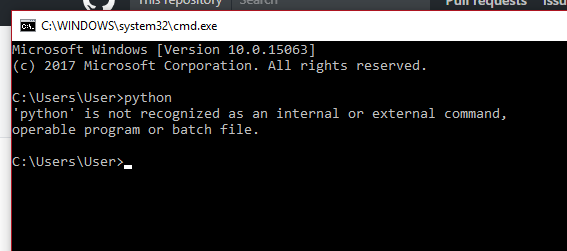
\includegraphics[width=1\textwidth]{Plagiarisme/cmd.png}}
	\caption{Contoh skirpt pada command prompt.}
	\label{cmd}
	\end{figure}
Pada gambar \ref{cmd} memberitahukan bahwa pada komputer yang saya pakai sekarang ini belum ada atau belum terinstall python.
Ketika python belum terinstall maka sistem akan mendeteksi bahwa comand yang diberikan tidak cocok dengan yang ada disistem. 
Akan tetapi kalau sudah terinstall maka akan memunculkan nama python begitu pula versi python yang di install.
Python menyediakan dukungan yang kuat untuk integrasi dengan bahasa pemrograman lain dan alat-alat bantu lainnya. 
Python hadir dengan pustakapustaka standar yang dapat diperluas serta dapat dipelajari hanya dalam beberapa hari.
Sudah banyak programmer Python yang menyatakan bahwa mereka mendapatkan produktivitas yang lebih tinggi. 
Mereka juga merasakan bahwa Python meningkatkan kualitas 
\begin{verbatim}
#!/usr/bin/python
import sys
try:
   # open file stream
   file = open(file_name, "w")
except IOError:
   print "There was an error writing to", file_name
   sys.exit()
print "Enter '", file_finish,
print "' When finished"
while file_text != file_finish:
   file_text = raw_input("Enter text: ")
   if file_text == file_finish:
      # close the file
      file.close
      break
   file.write(file_text)
   file.write("\n")
file.close()
file_name = raw_input("Enter filename: ")
if len(file_name) == 0:
   print "Next time please enter something"
   sys.exit()
try:
   file = open(file_name, "r")
except IOError:
   print "There was an error reading file"
   sys.exit()
file_text = file.read()
file.close()
print file_text
\end{verbatim}

\subsection{Memasang Phyton}
Distribusi Python tersedia untuk berbagai macam platform. Anda hanya perlu mendownload kode biner yang berlaku untuk platform 
Anda dan menginstal Python.
Jika kode biner untuk platform Anda tidak tersedia, Anda memerlukan kompiler C untuk mengkompilasi kode sumber secara manual. 
Kompilasi kode sumber menawarkan fleksibilitas lebih dalam hal pilihan fitur yang Anda butuhkan dalam instalasi Anda.
Berikut adalah ikhtisar singkat tentang menginstal Python di berbagai platform :

\subsection{Menyiapkan PATH}
Program dan file eksekusi lainnya bisa berada di banyak direktori, 
jadi sistem operasi menyediakan jalur pencarian yang mencantumkan direktori yang dicari OS untuk executable.
Path disimpan dalam variabel lingkungan, yang merupakan string bernama yang dikelola oleh sistem operasi. 
Variabel ini berisi informasi yang tersedia untuk perintah shell dan program lainnya.
The path variabel disebut sebagai PATH di Unix atau jalan pada Windows (Unix adalah kasus sensitif, Windows tidak).
Di Mac OS, installer menangani detail jalur. Untuk meminta juru bahasa Python dari direktori tertentu, 
Anda harus menambahkan direktori Python ke path Anda.

\subsection{installasi Python pada windows}
	\begin{enumerate}
	\item Unduh Python 2.7 di python.org.
	\item Jalankan file instalasi Python yang telah diunduh. Secara default Python akan terinstall di folder C:>Python27.
	\item Selanjutnya mengatur variable environment, buka Control Panel->System and Security->System.
	\item Klik Advanced system settings, Environment Variables.
	\item Pada System variables, pilih Path, klik Edit.
	\item Pada Variable value, tambahkan ;C: Python27.
	\end{enumerate}
	
\subsubsection{Pengujian Python pada windows}
	\begin{enumerate}
	\item Cara pertama: ketik python untuk menjalankan Python Interpreter. 
	      Jika berhasil akan ditampilkan versi Python yang digunakan beserta interpreternya. 
	      Coba ketikkan print “hello world” untuk menampilkan teks hello world.
	\item Cara kedua: buat file hello.py, yang isinya print “hello world”, 
	      simpan di mana saja suka-suka kamu, misalnya di D: python-code. Buka command prompt, Run -> cmd. 
	      Kemudian masuk ke folder D: python-code, lalu ketik python hello.py untuk menjalankan file Python yang telah dibuat.
	\end{enumerate}

\subsection{Installasi Python pada Unix/Linux}
	Berikutini adalah simple steps untuk menginstall python pada Unix/Linux.
	\begin{enumerate}
	\item Buka web browser dan ketik alamat https://www.python.org/downloads/
	\item Ikuti link untuk mendownload source code yang bisa digunakan oleh Unix/Linux
	\item Download dan kemudian extrak file
	\item Edit modules/setup file jika mau customize beberapa pengaturan
	\item Jalankan perintah ./configure script
	\item Installasi 
	\end{enumerate}
Lokasi standar penginstallan python ada pada /usr/local/bin dan libraries nya berada 
/usr/local/lib/pythonXX dimana XX adalah versi python yang di install.

\subsection{Setting Path pada Unix/Linux}
Untuk menambahkan direktori python di path pada Unix
\begin{enumerate}
\item In the csh shell – ketik setenv PATH PATH:/usr/local/bin/python lalu tekan enter
\item In the bash shell(Linux) – ketik export ATH=PATH:/usr/local/bin/python lalu tekan enter
\item In the sh or ksh shell – ketik PATH=PATH:/usr/local/bin/python lalu tekan enter
\item Note - /usr/local/bin/python adalah path untuk direktori Python
\end{enumerate}

\subsection{Fitur Python}
Fitur-Fitur Python Python memiliki beberapa fitur yang menjadikan bahasa pemrograman ini berbeda dari bahasa lain antara lain :
\begin{enumerate}
\item Memiliki kepustakaan yang luas, dalam distribusi Python telah disediakan modul- modul siap pakai untuk berbagai keperluan.
\item Memiliki tata bahasa yang jernih dan mudah dipelajari.
\item Memiliki aturan layout kode sumber yang memudahkan
\item pengecekan, pembacaan kembali dan penulisan ulang kode sumber.
\item Berorientasi obyek.
\item Memiliki sistem pengelolaan memori otomatis (garbage collection, seperti java) Modular, mudah dikembangkan dengan menciptakan modul-modul baru; modul- modul tersebut dapat dibangun dengan bahasa Python maupun C/C++.
\item Memiliki fasilitas pengumpulan sampah otomatis, seperti halnya pada bahasa pemrograman Java, python memiliki fasilitas pengaturan penggunaan memory komputer sehingga para pemrogram tidak perlu melakukan pengaturan memory komputer secara langsung.
\item Memiliki banyak faslitas pendukung sehingga mudah dalam pengoprasiannya.
\end{enumerate}

\subsection{Pengujian}
Cara pertama: ketik python untuk menjalankan Python Interpreter. Jika berhasil akan ditampilkan versi Python yang digunakan beserta interpreternya. Coba ketikkan print “hello world” untuk menampilkan teks hello world.

C:$>$python
Python 2.7.11 (v2.7.11:6d1b6a68f775, Dec  5 2015, 20:40:30) [MSC v.1500 64 bit (AMD64)] on win32
Type "help", "copyright", "credits" or "license" for more information.

$>$$>$$>$  print "hello world"

$>$$>$$>$ hello world



\subsection{Alasan Menggunakan Phyton}

Python memiliki konsep desain yang bagus dan sederhana, yang berfokus pada kemudahan dalam penggunaan. Kode Python dirancang untuk mudah dibaca, dipelajari, digunakan ulang, dan dirawat. Selain itu, Python juga mendukung pemograman berorientasi objek dan pemograman fungsional.


\subsection{Tipe Data Phyton}
	Menggunakan tipe Number

Tipe data Number digunakan untuk menyimpan nilai-nilai numerik. Tipe ini merupakan tipe data immutable, yang artinya jika kita mengubah nilai dari sebuah data, maka kita akan mengalokasikan obyek baru. Sama seperti tipe data lainnya, obyek Number dibuat ketika kita memberikan sebuah nilai padanya. Contoh:

$>$$>$$>$ data = 1

Kita juga dapat mengubah nilai yang ada dalam variable data tersebut.

$>$$>$$>$ data = data + 1

$>$$>$$>$ data=3.50

$>$$>$$>$ floatdat = 7.5

$>$$>$$>$ data = floatdat

Kita dapat menghapus sebuah obyek ataupun banyak obyek dengan menggunakan pernyataan del. Misalnya:

$>$$>$$>$ del data

$>$$>$$>$ del data, floatdat

Python mengelompokkan tipe Number dalam 4 macam, yaitu:

Plain Integer
Plain integer atau bilangan bulat merupakan tipe data yang sering kita temui pada semua bahasa pemrograman. Integer ini mempunyai range nilai antara $-2^32$ sampai $2^31 – 1$. Tipe ini juga dapat ditulis dalam bentuk octal (di tanda awalan “0”) maupun hexadesimal (ditandai awalan “0x” atau “0X”). Contoh:
10 100 6542 -784
083 -042 -0x43 0X61

Long Integer
Long integer sangat membantu kita untuk perhitungan di luar range nilai integer. Secara virtual, tidak ada batasan nilai tergantung besar virtual memory yang kita gunakan. Akhiran ‘l‘ atau ‘L‘ disetiap nilai bilangan bulat menandakan bahwa data tersebut bertipe long integer.
562718819L -0x526718L 012L -567299101L

Floating Point Real Number
Tipe ini sering disebut sebagai tipe real (atau float). Tipe ini sama dengan tipe double di C. Nilai float mempunyai dua bagian, bagian titik desimal dan bagian eksponensial. Tanda positif atau negatif diantara “e” merupakan tanda eksponen. Contoh nilai float:
0.0 14.5 -15.4 32.3+e18
-90.76712 -90. -32.54e100 70.2-E12

Complex Number
Sebuah bilangan kompleks biasanya ditunjukkan oleh bentuk a + bj, dimana a adalah bagian real dan b adalah bagian imajiner. Bagian imajiner merupakan bilangan di awal tanda “j” atau “J“. Berikut ini contoh bilangan kompleks:
3.14j 45j 54.56+12.1J 3e+36J

Bagian real dan imajiner dari bilangan kompleks dapat kita pisahkan menggunakan data atribut, yaitu menggunakan real dan imag. Sedangkan untuk mendapatkan konjugasi dari bilangan kompleks tersebut, kita dapat menggunakan metode conjugate().

$>$$>$$>$ kompleks = 23.45-1.23J

$>$$>$$>$  kompleks.real

23.45

$>$$>$$>$  kompleks.imag

-1.23

$>$$>$$>$ kompleks.conjugate()

(23.45+1.23j)

String merupakan salah satu tipe data yang sering digunakan dalam pemrograman Python. Sebuah string dapat dinyatakan sebagai kumpulan karakter yang dibatasi oleh satu atau dua tanda petik. Inilah contohnya,

$>$$>$$>$ nama = "Rolly Maulana Awangga"

$>$$>$$>$ nama

'Rolly Maulana Awangga'

$>$$>$$>$ slm = 'Salam Python Dahsyat!'

$>$$>$$>$ slm

'Salam Python Dahsyat!'

$>$$>$$>$ print slm

Salam Python Dahsyat!

Dari contoh di atas, ketika kita memanggil variabel secara langsung maka akan ditampilkan isi dari variabel tersebut dengan sebuah tanda petik. Namun jika kita menggunakan pernyataan print, maka tanda petik tersebut akan dihilangkan.

Menampilkan Tanda Petik Sebagai String

Di dalam sebuah string tidak dapat berisi tanda petik yang sama dengan tanda petik yang digunakan oleh string tersebut. Misalkan, ketika kita menuliskan 'Py'thon' maka akan muncul pesan kesalahan (syntax error). Agar tidak muncul pesan kesalahan, kita bisa mengganti tanda petik luarnya dengan tanda petik ganda, misalnya "Py'thon". Tanda petik juga dapat ditulis setelah tanda backslash agar dapat ditampilkan sebagai string.

$>$$>$$>$ str = "Py'thon"

$>$$>$$>$ str

"Py'thon"

$>$$>$$>$  str2 = 'Py"thon'

$>$$>$$>$ str2

'Py"thon'

$>$$>$$>$ "\"OK, \" sampai ketemu lagi."

'"OK, " sampai ketemu lagi.'

Kode n atau Triple Quotes Juga Boleh!

Jika kita ingin menuliskan string yang panjang dalam beberapa baris, maka kita perlu menambahkan tanda backslash diikuti huruf n (n) sebagai tanda baris baru.

$>$$>$$>$ teks = "Python adalah bahasa pemrograman yang powerfull.nTerbukti Python bisa dijalankan di segala platform OS.nJadi, saatnya kita menggunakan Python sebagai bahasa permrograman nsehari-hari. Salam Python Dahsyat!"

Tanda n akan memberikan perintah membuat baris baru jika kita memanggil teks dengan pernyataan print.

$>$$>$$>$ print teks

Python adalah bahasa pemrograman yang powerfull.
Terbukti Python bisa dijalankan di segala platform OS.
Jadi, saatnya kita menggunakan Python sebagai bahasa permrograman
sehari-hari. Salam Python Dahsyat!

Kita juga dapat menggunakan tanda petik tiga (triple quotes), """ atau ''', untuk menuliskan sebuah string yang panjang dalam beberapa baris.

$>$$>$$>$ teks = """Python adalah bahasa pemrograman yang powerfull.
... Terbukti Python bisa dijalankan di segala platform OS.
... Jadi, saatnya kita menggunakan Python sebagai bahasa pemrograman
... sehari-hari. Salam Python Dahsyat!"""

Tampilan teks dengan pernyataan print seperti di bawah ini,

$>$$>$$>$ print teks
Python adalah bahasa pemrograman yang powerfull.
Terbukti Python bisa dijalankan di segala platform OS.
Jadi, saatnya kita menggunakan Python sebagai bahasa pemrograman
sehari-hari. Salam Python Dahsyat!

Menggabungkan String

Untuk menggabungkan dua buah string atau lebih, kita dapat menggunakan operator +. Sedangkan untuk menggandakan string, kita gunakan operator *.

$>$$>$$>$ Tampan = 'Rolly' + 'Ganteng'

$>$$>$$>$ Tampan
'RollyGanteng'

$>$$>$$>$ newTampan = Tampan*5

$>$$>$$>$ newTampan

'RollyGantengRollyGantengRollyGantengRollyGantengRollyGanteng'

$>$$>$$>$ Tampan *= 4

$>$$>$$>$ print Tampan

RollyGantengRollyGantengRollyGantengRollyGanteng

Jika dua string ditulis secara berurutan, maka secara langsung kedua string tersebut akan digabungkan.

$>$$>$$>$ Tampan = 'Rolly''Ganteng'

$>$$>$$>$ Tampan

'RollyGanteng'

Menentukan Panjang String

Panjang dari sebuah string dapat kita temukan dengan menggunakan fungsi len().

$>$$>$$>$ len(blog)
12

Memecah String

Tidak seperti bahasa lainnya, Python tidak mendukung tipe Karakter. Untuk mengambil satu karakter atau lebih dari sebuah string, kita dapat memecah string tersebut menggunakan indeks (disebut Metode Irisan). Irisan terdiri dari dua indeks yang dipisahkan tanda koma.

$>$$>$$>$ buah = 'Nanas'

$>$$>$$>$ buah[0]

'N'

$>$$>$$>$ buah[0:2]

'Na'

$>$$>$$>$ buah[0:4]

'Nana'

$>$$>$$>$ buah[0:5]

'Nanas'

Dari contoh di atas, panjang string buah adalah 5. Ketika kita menghitung maju, indeks bernilai 0 sampai (panjang-string – 1) dimulai dari kiri ke kanan. Maka dari itu, kita dapat mengakses setiap karakter dalam range 0 sampai 4.

Sebuah string juga dapat dihitung mundur, dengan indeks -1 sampai (negatif panjang-string) dimulai dari kanan ke kiri. Berikut gambaran lengkapnya, baik itu penghitungan maju atau mundur.

Contoh penggunaan penghitungan mundur,

$>$$>$$>$ buah[-1]

‘s’

$>$$>$$>$ buah[-5]

‘N’

$>$$>$$>$ buah[-5:-1]

‘Nana’

$>$$>$$>$ buah[1:-1]

‘ana’

Jika kita lupa berapa nilai indeks awala atau indeks akhir, kita dapat kosongkan indeks tersebut.

$>$$>$$>$ buah[:3]

‘Nan’

$>$$>$$>$ buah[2:]

‘nas’


Pengosongan indeks akan menyebabkan semua string ditampilkan.

$>$$>$$>$ buah[:]

‘Nanas’

String Bersifat Immutable

Tipe data String pada Python bersifat immutable, yang artinya sekali dibuat maka tidak dapat diubah kembali. Ada pertanyaan bagus, jika string bersifat immutable, mengapa kita bisa mengubah nilai dari variabel string tersebut? Jawabannya sangat sederhana. Ketika kita memberikan nilai yang berbeda pada variabel string, sebuah obyek baru berhasil kita buat. Lihat contoh berikut,

$>$$>$$>$ nama = "Klinik"

$>$$>$$>$ nama

'Klinik'

$>$$>$$>$ id(nama)

3076962016L

$>$$>$$>$ nama = "Python"

$>$$>$$>$ id(nama)

3077289888L

Catat bahwa ketika string nama telah kita buat, maka identitas dari variabel ini dapat kita ketahui dengan menggunakan fungsi id(). Jika kita ubah nilai dari variabel nama tersebut, maka identitasnya juga berubah. Hal ini menandakan bahwa obyek baru telah dibuat. Penggantian nilai pada string pada posisi indeks tertentu akan menghasilkan pesan kesalahan.

$>$$>$$>$ nama[0] = 'K'

Traceback (most recent call last):

File "", line 1, in

TypeError: 'str' object does not support item assignment

Kita juga dapat menambahkan sebuah string baru pada string lama.

$>$$>$$>$ 'Si' + nama[0]

'SiP'

$>$$>$$>$ 'J' + nama[1:]

'Jython'



\chapter{Basic Syntax}
% Tugas 3 Kelompok 4
% Akbar Pambudi Utomo (1154094)
% Julham Ramadhana (1154069)
% Pebridayanti Hasibuan (1154118)
% Andi Nurfadillah Ali (1154041)



\section{Basic Syntax}
\subsection{Pengenal Python}
Pengenal Python Pengenal Python adalah nama yang digunakan untuk mengidentifikasi variabel, fungsi, kelas, modulatauobjeklainnya. Pengenal dimulai dengan huruf A sampai Z atau huruf a sampai z atau garis bawah  diikuti oleh nol atau lebih huruf, garis bawah dan angka (0 sampai 9). Python tidak mengizinkan karakter tanda baca seperti \@, \$, dan \% dalam pengenal. Python adalah bahasa pemrograman yang sensitif. Dengan demikian, Tenaga Kerja dan Tenaga Kerja adalah dua pengidentifikasi yang berbeda dengan Python. Berikut adalah konvensi penamaan untuk pengenal Python - Nama kelas dimulai dengan huruf besar. Semua pengenal lainnya mulai dengan huruf kecil. Memulai pengenal dengan satu garis bawah terkemuka menunjukkan bahwa pengenal bersifat pribadi. Memulai pengenal dengan dua garis bawah terkemuka menunjukkan pengenal yang sangatpribadi. Jika pengenal juga diakhiri dengan dua tanda garis bawah, identifier adalah nama khusus yang ditentukan bahasa. 
Bahasa Python memiliki banyak kesamaan dengan Perl, C, dan Java. Namun, ada beberapa perbedaan yang pasti antara bahasa. Program Python Pertama Mari kita jalankan program dalam mode pemrograman yang berbeda. Pemrograman Mode Interaktif Memohon interpreter tanpa melewatkan file script sebagai parameter menampilkan prompt berikut :
	\begin{verbatim}
		Python

		Python 2.4.3 (#1, Nov 11 2010, 13:34:43) 
		[GCC 4.1.2 20080704 (Red Hat 4.1.2-48)] on linux2 Type ”help”, ”copyright”, ”credits” or ”license” for more information.
		
		Ketik teks berikut pada prompt Python dan tekan Enter:
		Python 2.4.3 ( #1, Nov 11 2010, 13:34:43) 
		[GCC 4.1.2 20080704 (Red Hat 4.1.2-48)] 
		on linux2 Type ”help”, ”copyright”, 
		”credits” or ”license” for more information.

		Ketik teks berikut pada prompt Python dan 
		tekan Enter:

		
		print ”Hello, Python!”
	\end{verbatim}

Jika Anda menjalankan versi baru Python, Anda perlu menggunakan pernyataan cetak dengan tanda kurung seperti pada cetak \verb|(”Halo,Python!”);|. Namun dengan versi Python 2.4.3, ini menghasilkan hasil sebagai berikut:

Hello, Python!

\subsection{Pemrograman Mode Script}
Memohon interpreter dengan parameter script memulai eksekusi script dan berlanjut sampai script selesai. Saat skrip selesai, juru bahasa tidak lagi aktif. Mari kita tuliskan program Python sederhana dalam sebuah naskah. File Python memiliki ekstensi .py. Ketik kode sumber berikut di file.
Objek Dengan Python, seperti semua bahasa berorientasi objek, ada kumpulan kode dan data yang disebut objek, yang biasanya mewakili potongan dalam model konseptual suatu sistem. Objek dengan Python dibuat (yaitu, instantiated) dari template yang disebut kelas (yang akan dibahas kemudian, sebanyak bahasa dapat digunakan tanpa memahami kelas). Mereka memiliki atribut, yang mewakili berbagai potongan kode dan data yang membentuk objek. Untuk mengakses atribut, seseorang menuliskan nama objek yang diikuti oleh suatu periode (selanjutnya disebut titik), diikuti dengan nama atribut.
Contohnya adalah atribut ’atas’ dari string, yang mengacu pada kode yang mengembalikan salinan string di mana semua huruf adalah huruf besar. Untuk mendapatkan ini, perlu untuk memiliki cara untuk merujuk ke objek (dalam contoh berikut, jalan adalah string literal yang membangun objek).

\subsection{Pengertian Python}
Python adalah salah satu pemrograman yang terus berkembang dan bertahan dikarenakan dukungan komunitas yang aktif diseluruh dunia. Banyak forum-forum ataupun blogger-blogger yang sering membagi pengalaman dalam menggunakan python. Hal ini memudahkan bagi pengguna pemula maupun pengembang untuk bertanya dan sharing tentang ilmu pemrograman ini. 
\begin{figure} [ht]
	\centerline{
\includegraphics[width=1\textwidth]{Plagiarisme/logopython.jpg}}
	\caption{Gambar Logo Python}
	\label{logopython}
	\end{figure}
Gambar berikut \ref{logopython} adalah gambar logo python dengan lambang 2 ular python yang saling membelakangi. ular diatas berwarna biru dan ular dibawah berwarna kuning. 

\subsection{Kelebihan dan Kekurangan Python}
Kelebihan yang dimiliki oleh Python :
	\begin{itemize}
		\item Tidak ada tahapan kompilasi dan penyambungan (link) sehingga kecepatan perubahan pada masa pembuatan sistem aplikasi meningkat. 
		\item Tidak ada deklarasi tipe data yang merumitkan sehingga program menjadi lebih sederhana, singkat, dan fleksible. 
		\item Manajemen memori otomatis yaitu kumpulan sampah memori sehingga dapat menghindari pencacatan kode. 
		\item Tipe data dan operasi tingkat tinggi yaitu kecepatan pembuatan sistem aplikasi menggunakan tipe objek yang telah ada. 
		\item Pemrograman berorientasi objek.
		\item Pelekatan dan perluasan dalam C. 
		\item Terdapat kelas, modul, eksepsi sehingga terdapat dukungan pemrograman skala besar secara modular.
		\item Pemuatan dinamis modul C sehingga ekstensi menjadi sederhana dan berkas biner yang kecil 
		\item Pemuatan kembali secara dinamis modul phyton seperti memodifikasi aplikasi tanpa menghentikannya. 
		\item Model objek universal kelas Satu. 
		\item Konstruksi pada saat aplikasi berjalan.
		\item Interaktif, dinamis dan alamiah. 
		\item Akses hingga informasi interpreter. 
		\item Portabilitas secara luas seperti pemrograman antar platform tanpa ports. 
		\item Kompilasi untuk portable kode byte sehingga kecepatan eksekusi bertambah dan melindungi kode sumber.
		\item Antarmuka terpasang untuk pelayanan keluar seperti perangkat Bantu system, GUI, persistence, database, dll. 
	\end{itemize}
Kekurangan yang dimiliki Python :
	\begin{itemize}
		\item Beberapa penugasan terdapat diluar dari jangkauan python, seperti bahasa pemrograman dinamis lainnya, python tidak secepat atau efisien sebagai statis, tidak seperti bahasa pemrograman kompilasi seperti bahasa C. 
		\item Disebabkan python merupakan interpreter, python bukan merupakan perangkat bantu terbaik untuk pengantar komponen performa kritis. 
		\item Python tidak dapat digunakan sebagai dasar bahasa pemrograman implementasi untuk beberapa komponen, tetapi dapat bekerja dengan baik sebagai bagian depan skrip antarmuka untuk mereka. 
		\item Python memberikan efisiensi dan fleksibilitas tradeoff by dengan tidak memberikannya secara menyeluruh. Python menyediakan bahasa pemrograman optimasi untuk kegunaan, bersama dengan perangkat bantu yang dibutuhkan untuk diintegrasikan dengan bahasa pemrograman lainnya.
		\item Banyak terdapat referensi lama terutama dari pencarian google, python adalah pemrograman yang sangat lambat. Namun belum lama ini ditemukan bahwa Google, Youtube, DropBox dan beberapa software sistem banyak menggunakan Python.
	\end{itemize}
Dibalik kelebihan dan kekurangan yang dimiliki, Kini Python menjadi salah satu bahasa pemrograman yang populer digunakan oleh pengembangan web, aplikasi web, aplikasi perkantoran, simulasi, dan masih banyak lagi. Hal ini disebabkan karena Python bahasa pemrograman yang dinamis dan mudah dipahami. Python memiliki hak cipta. Seperti Perl, kode sumber Python sekarang tersedia di bawah GNU General Public License (GPL). Python sekarang dikelola oleh tim pengembangan inti di institut tersebut, walaupun Guido van Rossum masih memegangperanpentingdalammengarahkankemajuannya.

\subsection{Fitur Python}
Python memiliki fitur yang meliputi:
	\begin{enumerate}
		\item Mudah dipelajari: Python memiliki beberapa kata kunci, struktur sederhana, dan sintaks yang jelas. Hal ini memungkinkan siswa untuk mengambil bahasa dengan cepat.
		\item Mudah dibaca: kode Python lebih jelas dan terlihat oleh mata.
		\item Mudahdipelihara: kodesumberPythoncukupmudahuntuk dipelihara.
		\item Perpustakaan standar yang luas: sebagian besar perpustakaan Python sangat portabel dan kompatibel dengan platformcross-platformdiUNIX,Windows,danMacintosh. 
		\item Mode Interaktif: Python memiliki dukungan untuk mode interaktif yang memungkinkan pengujian interaktif dan debugging dari cuplikan kode.
		\item Portable: Python dapat berjalan di berbagai platform perangkat keras dan memiliki antarmuka yang sama pada semua platform.
		\item Dapat diperpanjang: Anda dapat menambahkan modul tingkat rendah ke penerjemah Python. Modul ini memungkinkan programmer untuk menambahkan atau menyesuaikan alat mereka agar lebih efisien.
		\item Database: Python menyediakan antarmuka untuk semua database komersial utama. 
	\end{enumerate}

\subsection{Fitur Python}
Fitur Python meliputi:
	\begin{enumerate}
		\item Mudah dipelajari: Python memiliki beberapa kata kunci, struktur sederhana, dan sintaks yang jelas. Hal ini 			memungkinkan siswa untuk mengambil bahasa dengan cepat.
		\item  Mudah dibaca: kode Python lebih jelas dan terlihat oleh mata.
		\item  Mudah dipelihara: kode sumber Python cukup mudah untuk dipelihara. Perpustakaan standar yang luas: sebagian besar 		perpustakaan. Python sangat portabel dan kompatibel dengan
		platform cross-platform di UNIX,Windows, dan Macintosh.
		\item Mode Interaktif: Python memiliki dukungan untuk mode interaktif yang memungkinkan pengujian interaktif dan 			debugging dari 	cuplikan kode.
		\item Portable: Python dapat berjalan di berbagai platform perangkat keras dan memiliki antarmuka yang sama pada semua 			platform.
		\item  Dapat diperpanjang: Anda dapat menambahkan modul tingkat rendah ke penerjemah Python. Modul ini memungkinkan 			programmer untuk menambahkan atau menyesuaikan
		alat mereka agar lebih efisien.
		\item  Database: Python menyediakan antarmuka untuk semua database komersial utama.
	\end{enumerate}



\subsection{Pernyataan Multi-Line}
Pernyataan di Python biasanya diakhiri dengan baris baru. Python, bagaimanapun, memungkinkan penggunaan karakter kelanjutan baris (\\)\ untuk menunjukkan bahwa garis tersebut harus dilanjutkan. Misalnya –
	\begin {verbatim}
\subsection {Pernyataan Multi-Line}
Pernyataan di Python biasanya diakhiri dengan baris baru. Python, bagaimanapun, memungkinkan penggunaan karakter kelanjutan baris untuk menunjukkan bahwa garis tersebut harus dilanjutkan. Misalnya –
	\begin {equation}

	total = item_one + \
		item_two + \
		item_three
	\end {verbatim}

Pernyataan yang ada di dalam kurung [], {}, atau () tidak perlu menggunakan karakter kelanjutan baris. Misalnya –

	\begin{verbatim}
	days = ['Monday', 'Tuesday', 'Wednesday',
		'Thursday', 'Friday']
	\end{verbatim}

\subsection{Kutipan pada Python}
Python menerima kutipan tunggal \verb|('), ganda (") dan triple (' '' atau '" ")| untuk menunjukkan literal string, selama jenis kutipan yang sama dimulai dan mengakhiri string.
Tanda kutip triple digunakan untuk membentang string di beberapa baris. Misalnya:
	\begin{verbatim}
	word = 'word'
	sentence = "This is a sentence."
	paragraph = """This is a paragraph. It is
	made up of multiple lines and sentences."""
	\end {verbatim}

\subsection{Komentar pada Python}
Tanda hash (\#)\ yang tidak berada di dalam string literal memulai sebuah komentar. Semua karakter setelah \#\ dan sampai akhir garis fisik adalah bagian dari komentar dan penafsir Python mengabaikannya.
	\begin{verbatim}
	#!/usr/bin/python

	# First comment
	print \"Hello, Python!\" # second comment
	\end{verbatim}

	 Dan hasilnya sebagai berikut :
	
	    Hello, Python!


Anda bisa mengetikkan komentar di baris yang sama setelah sebuah pernyataan atau ungkapan –
	\begin{verbatim}
	    name = \"Madisetti\" # This is again comment
	\end{verbatim}

Anda dapat mengomentari beberapa baris sebagai berikut –
	\begin{verbatim}
	# This is a comment.
	# This is a comment, too.
	# This is a comment, too.
	# I said that already.
	\end{verbatim}

\subsubsection{Variabel}	
	\begin{equation}
	days = ['Monday', 'Tuesday', 'Wednesday',
		'Thursday', 'Friday']
	\end{equation}
	
\subsection{Kutipan pada Python}
Python menerima kutipan tunggal ('), ganda (") dan triple (' '' atau '" ") untuk menunjukkan literal string, selama jenis kutipan yang sama dimulai dan mengakhiri string.
Tanda kutip triple digunakan untuk membentang string di beberapa baris. Misalnya:
	\begin{equation}
	word = 'word'
	sentence = "This is a sentence.
	\end{equation}

\subsection{Komentar pada Python}
Tanda hash yang tidak berada di dalam string literal memulai sebuah komentar. Semua karakter setelah dan sampai akhir garis fisik adalah bagian dari komentar dan penafsir Python mengabaikannya.
	\begin{equation}
	!/usr/bin/python
	print "Hello, Python!" 
	\end{equation}

	 Dan hasilnya sebagai berikut –
	\begin{equation}
	    Hello, Python!
	\end{equation}

Anda bisa mengetikkan komentar di baris yang sama setelah sebuah pernyataan atau ungkapan –
	\begin{equation}
	    name = "Madisetti"  This is again comment
	\end{equation}

Anda dapat mengomentari beberapa baris sebagai berikut –
	\begin{equation}
	This is a comment.
	I said that already.
	\end{equation}
	
	

\subsection{Variabel}	

 Jadi variable itu untuk menyimpan data sebagai penampung nya dan nilai adalah isi dari variable itu sendiri.
Contoh variable katakana saja my int = 7 itu juga bisa di ubah menjadi my int =3  
Code merubah nilai variablenya  
	My int = 7
	My int = 
	Print my int 

\subsection{Whitespace} 
Whitespace adalah penyusun kode untuk penulisan oleh karena itu harus berhati hati karena sangat sensitive
Contoh code nya: 
 \begin{verbatim}
 	Def spam() 
	Eggs + 12 
 	Return eggs 
 	Print spam()
 \end{verbatim}
Itu merupakan kode penulisan yang salah maka akan muncul pesan error.
Pesan error yang muncul tentang penulisan dan bisa di edit agar tidak terjadi kesalahan penulisan lagi.
Contoh yang benar :  
 \begin{verbatim}
 	Def spam(): 
 	Eggs = 12 
 	Return eggs 
 	Print spam() 
 \end{verbatim}
Kita coba contohkan penulisan oprasi matematika nya.
Code nya adalah: 
 \begin{verbatim}	
	Jumlah = 10+10 
	Print jumlah 
	Pejumlahan = 72 + 23 
	Pengurangan 108 – 204 
	Perkalian = 108 * 0,5 
	Pembagian = 108 / 9 
 \end{verbatim}
Maka akan muncul print yang sesuai inputan yang kalian buat. 
Selain itu bisa juga perpangkatan 

Kalkulator pangkatan meggunakan eight 

Contohnya \verb|eight = \2** 3\| 

Eight itu adalah variable baru yang kita buat untuk mengeset nilai menjadi 8.

Contoh: stopwatch sederhana yang biasa nya di gunakan untuk ujian peraktek.  
Penjelasan tentang stopwatch yaitu alat untuk mengukur kecepatan suatu benda secara akurat. 
Sebelum membuat nya kita harus mengetahui cara kerja stopwatch itu sendiri. Memulai angka nya dari 0 karena angka 0 adalah angka pertama dalam waktu.
Code nya antara lain:
 \begin{verbatim}
	Depanjam = 0 
	Jam = 0 
	Depanmenit = 0 
	Menit = 0 
	Depandetik = 0 
	Detik = 0
 \end{verbatim}
Lalu gunakan import time 
Untuk system loop jadi setelah detik mencapai 9 maka menit akan bertambah 1 seperti itu. 
 \begin{verbatim}
	While true : 
	Time.sleep(1) 
	Detik += 1 
	If detik == 9: 
	Detik = 0 
	Depandetik += 1 
	If depandetik == 6:
	Menit +=1 
	Depandetik = 0 
	Detik = 0 
	If menit == 9: 
	Menit = 0 
	Depanmenit += 1 
	If depanmenit == 6: 
	Jam +=1 
	Depanmenit = 0 
	Menit = 0 
	If ja, == 9 : 
	Depanjam += 1 
	Jam = 0 
Print ( $ " $ $  {  $0 $  }  $ $  {  $1 $  }  $ $  {  $2 $  }  $ $  {  $3 $  }  $ $  {  $4 $  }  $ $  {  $5 $  vert  $ $  }  $ $ " $. Format(Depanjam,Jam,Depanmenit,Menit,Depandetik,Detik), end= $ " $ $  setminus  $r $ " $) 
\end{verbatim}
Run maka akan jadi program simple tentang stopwatch sederhana.



\chapter{Variabel Type}
% Tugas 3 kelompok 4
% Julham Ramadhana (1154069)
% Akbar Pambudi Utomo (1154094)
% Hanna Theresia Siregar (1154009)
% Pebridayanti Hasibuan (1154118)
% Andi Nurfadllah Ali (1154041)
% Andi Wadi Afryandika (1154115)

\section{Python Variabel Type}
Satu dari fitur yang paling powerful dari sebuah bahasa pemrograman adalah kemampuan untuk memanipulasi variabel. Sebuah variabel adalah nama yang merujuk ke sebuah nilai. Variabel tidak lain hanyalah lokasi memori yang dipesan untuk menyimpan nilai. Ini berarti bahwa ketika kita membuat variabel, maka kita memesan beberapa ruang di memori. Berdasarkan tipe data sebuah variabel, penafsir mengalokasikan memori dan memutuskan apa yang dapat disimpan dalam memori yang dipesan. Oleh karena itu, dengan menetapkan tipe data yang berbeda ke variabel, kita dapat menyimpan bilangan bulat, desimal atau karakter dalam variabel ini.
Pernyataan pemberian nilai(assigment statement) akan memberikan nilai pada variabel: 
\begin{verbatim}
pesan = "Apa kabar, bro ?" 
n = 17  
pi = 3.14159 
\end{verbatim}
Contoh diatas melakukan tiga pemberian nilai. Yang pertama memberikan nilai string \"Apa kabar, bro ?\" pada variabel bernama pesan. Yang Kedua memberikan nilai integer 17 kepada n, dan yang ketiga memberikan nilai bilangan floating-point 3.14159 kepada variabel dengan nama pi.
Token pemberian nilai, tanda =, agar tidak bingung jangan disamakan dengan tanda sama dengan, yang mana menggunakan token ==. Pernyataan pemberian nilai mengikat sebuah nama di sebelah kiri dari operator, dan nilainya, di sebelah kanannya. Inilah mengapa kamu akan mendapatkan error jika kamu menulis: 
\begin{verbatim}
17 = n 
File "<interactive input>", line 1 
SyntaxError: can't assign to literal 
\end{verbatim}
Ketika membaca atau menulis kode, katakan dalam hati \"n diberikan nilai 17\". Jangan katakan \"n sama dengan 17\".
Cara umum untuk merepresentasikan variabel pada kertas adalah dengan menulis namanya dengan tanda panah mengarah ke nilai variabelnya. Gambar jenis ini dinamakan state snapshot karena ia memperlihatkan state atau kondisi dari setiap variabel pada instan waktu tertentu. (Pikirkan ini sebagai variabel keadaan pikiran). Diagram ini memperlihatkan hasil dari pengeksekusian pernyataan pemberian nilai.
Jika kamu meminta interpreter untuk menilai sebuah variabel, ia akan menghasilkan nilai dari variabel terkait pada waktu sekarang.
'Apa kabar, bro ?' 
	n 
	17 
	pi  
	3.14159 
Kita menggunakan variabel-variabel pada program untuk mengingat hal-hal, misalnya skore terkini ketika sedang ada pertandingan sepak bola. Tapi variabel tetaplah variabel. Ini artinya mereka bisa berganti seiring waktu, sama halnya dengan papan skor pada pertandingan bola. Kamu bisa memberikan nilai pada variabel, dan kemudian memberikan nilai lainnya pada variabel yang sama. (Ini berbeda dari sudut pandang matematika. Pada matematika, jika kamu memberi 'x' nilai 3, itu tidak bisa mengubah link nilai menjadi nilai yang berbeda pada pertengahan perhitungan yang kamu lakukan!) 
\begin{verbatim}
	hari = "Kamis" 
	hari 
	'Kamis'
	hari = "Jumat" 
	hari 
	'Jumat' 
	hari = 21
	hari 
	21 
\end{verbatim}
Kamu akan menyadari kita mengubah nilai dari hari sebanyak tiga kali, dan ketika pemberian nilai yang ketiga kita bahkan membuatnya merujuk pada nilai yang berbeda tipe dari yang sebelumnya. 
Pemrograman itu kebanyakan tentang bagaimana komputer mengingat sesuatu, misal, Jumlah panggilan tak terjawab pada handphone mu,dan kemudian mengatur untuk memperbaharui atau merubah variabel ketika kamu melewatkan panggilan lainnya. 

\subsection{Nama Variabel dan Keywords}
	Nama variabel bisa ditulis panjang. Mereka bisa berisi huruf maupun digit angka, tapi harus diawali dengan huruf atau underscore. Meskipun dibolehkan untuk menggunakan huruf besar, tapi pada umumnya kita tidak menggunakannya. Jika kamu menggunakannya, ingat kalau besar kecilnya huruf itu berpengaruh. Wayandan dan wayan itu merupakan dua variabel yang berbeda.


Karakter underscore  bisa ada pada nama. Biasanya digunakan pada nama yang terdiri dari lebih dari satu kata, misalnya seperti \verb|nama atau hargajualproduk.|

Ada beberapa situasi yang mana nama yang diawali dengan underscore memiliki arti yang spesial, jadi aturan yang paling aman untuk pemula adalah memulai sebuah nama hanya dengan menggunakan huruf kecil.
Jika kamu memberikan variabel nama yang ilegal, kamu akan mendapatkan syntax error: 
\begin{verbatim}
	123doremi = "tiga not awal" 
	SyntaxError: invalid syntax 
	gaji  \$   = 1000000 
	SyntaxError: invalid syntax 
	class = "Kewirausahaan 121" 
	SyntaxError: invalide syntax 
\end{verbatim}


\subsection{Tipe data standar}
Data yang tersimpan dalam memori bisa bermacam-macam. Misalnya, usia seseorang disimpan sebagai nilai numerik dan alamatnya disimpan sebagai karakter alfanumerik. Python memiliki berbagai jenis data standar yang digunakan untuk menentukan operasi yang mungkin dilakukan pada mereka dan metode penyimpanan untuk masing-masingnya.

Python memiliki lima tipe data standar -
\begin{itemize}
	\item Angka
	\item Tali
	\item Daftar
	\item Tuple
	\item Kamus
\end{itemize}
123doremi adalah ilegal karena tidak dimulai dengan huruf. gaji \$ juga ilegal karena memakai karakter ilegal, tanda dollar seharusnya tidak boleh. Tapi apa yang salah dengan class ?
Ternyata karena class merupakan satu dari keyword (kata kunci) yang dimiliki Python. Keyword mendefinisikan aturan syntax bahasa dan struktur, dan maka dari itu tidak diperkenakan untuk digunakan sebagai nama variabel. 
Python memiliki tiga puluhan keyword (dan hingga kini Python masih meningkatkannya dengan memperkenalkan atau menghilangkan satu atau dua). 
Kamu mungkin berniat untuk menyimpan daftar ini untuk mempermudah. Jika si interpreter komplain mengenai satu sari nama variabel mu dan kamu tidak tahu mengapa demikian, lihatlah apakah nama variabel yang kamu buat masuk daftar diatas. Jika iya, ganti dengan nama yang lain.  
Programer umumnya memilih nama untuk variabel mereka agar memiliki arti dan bisa dimengerti oleh pembaca manusia \(--\) dengan demikian maka akan membantu si programer untuk mendokumentasikan, atau mengingat, apa gunanya variabel tersebut.  

Pemula biasanya bingung dengan maksud dari berguna untuk pembaca manusia dengan berguna untuk mesin atau komputer. Jadi mungkin mereka akan berpikir salah, bahwa ketika mereka memanggil beberapa variabel dengan nama average ataupi, itu akan dengain ajaib menghitung sebuah average / rata-rata, atau dengan ajaib tahu kalau pi memiliki nilai seperti 3.14159. Tidak ! Komputer tidak akan mengerti itu, komputer tidak akan mengerti apa yang kamu inginkan dari variabel hanya karena namanya unik. 

Jadi kamu mungkin akan menemui beberapa instruktur yang memang sengaja tidak memilih nama yang berarti ketika mereka mengajar pemula bukan karena kita tidak menganggap itu merupakan kebiasaan yang baik, tapi karena kita mencoba untuk menekankan ulang pesannya kepada kalian seorang programer  harus menulis sendiri kode program untuk menghitung average-nya, dan kamu harus menulis pernyataan pemberian nilai untuk memberikan nilai pada variabel pidengan nilai yang kamu inginkan. 

\subsection{Pernyataan}
	Sebuah pernyataan (statement) adalah perintah/instruksi yang bisa dieksekusi/dijalankan oleh Python interpreter. Hingga kini kita hanya baru melihat pernyataan pemberian nilai. Beberapa jenis lain dari pernyataan yang akan kita lihat dengan singkat adalah pernyataan  while, pernyataan for, pernyataan if, dan pernyataan import. (Ada banyak lagi yang lainnya!).
Ketika kamu mengetikan pernyataan pada command line, Python akan menjalankannya. Pernyataannya sendiri tidak menghasilkan hasil apapun. 
Variabel tidak lain hanyalah lokasi memori reserved untuk menyimpan nilai. Ini berarti bahwa ketika Anda membuat variabel Anda memesan beberapa ruang di memori.
Berdasarkan tipe data sebuah variabel, penafsir mengalokasikan memori dan memutuskan apa yang dapat disimpan dalam memori yang dipesan. Oleh karena itu, dengan menetapkan tipe data yang berbeda ke variabel, Anda dapat menyimpan bilangan bulat, desimal atau karakter dalam variabel ini.

\subsubsection{Variabel}
	Variabel adalah lokasi memori yang dicadangkan untuk menyimpan nilai-nilai. Ini berarti bahwa ketika Anda membuat sebuah variabel Anda memesan beberapa ruang di memori. Variabel menyimpan data yang dilakukan selama program dieksekusi, yang natinya isi dari variabel tersebut dapat diubah oleh operasi - operasi tertentu pada program yang menggunakan variabel.
Penulisan variabel Python sendiri juga memiliki aturan tertentu, yaitu : 
\begin{enumerate}
	\item Karakter pertama harus berupa huruf atau garis bawah/underscore.
 	\item Karakter selanjutnya dapat berupa huruf, garis bawah/underscore atau angka.
	\item Karakter pada nama variabel bersifat sensitif (case-sensitif). Artinya huruf kecil dan huruf besar dibedakan. 
	Sebagai contoh, variabel namaDepan dan namadepan adalah variabel yang berbeda.
\end{enumerate}
Untuk mulai membuat variabel di Python caranya sangat mudah, Anda cukup menuliskan variabel lalu mengisinya dengan suatu nilai dengan cara menambahkan tanda sama dengan \(=\) diikuti dengan nilai yang ingin dimasukan. 

\subsubsection{Menilai Ekspresi}
	Sebuah ekspresi merupakan perpaduan antara nilai, variabel, operator, dan pemanggilan fungsi. Jika kamu mengetik sebuah ekspresi pada Python prompt, maka si interpreter akan menilainya dan menampilkan hasilnya:
	\begin{verbatim}
		1 + 1 
		2 
		len(”hello”) 
		5 
	\end{verbatim}
Pada contoh ini len merupakan fungsi built-in yang ada di Python yang akan menghasilkan jumlah karakter dari sebuah string. Sebelumnya kita sudah melihat fungsi print dan type, jadi ini adalah contoh fungsi ketiga kita.
Proses penilaian dari sebuah ekspresi akan menghasilkan sebuah nilai, itulah mengapa ekspresi bisa ada di sisi sebelah kanan dari pernyataan pemberian nilai. Nilai dengan sendirinya adalah ekspresi sederhana, dan begitu juga variabel.
	\begin{verbatim}
		17
		17 
		y = 3.14 
		x = len(”hello”) 
		x 
		5 
		Y

		3.14
	\end{verbatim}
	
\subsubsection{Menetapkan Nilai ke Variabel}
	Variabel Python tidak memerlukan deklarasi eksplisit untuk memesan ruang memori. Deklarasi terjadi secara otomatis saat Anda menetapkan nilai ke variabel.Tanda sama \(=\) digunakan untuk menetapkan nilai pada variabel. 
Operand di sebelah kiri = operator adalah nama variabel dan operan di sebelah kanan = operator adalah nilai yang tersimpan dalam variabel.Misalnya:
\begin{verbatim}
	counter~=~100~~~~~~~    An integer assignment 
	miles~~~=~1000.0~~~~    A floating point 
	name~~~~=~"John"~~~~    A string 
	print counter 
	print miles 
	print name
\end{verbatim}
Di sini, 100, 1000.0 dan \"John\" adalah nilai yang diberikan untuk melawan, mil, dan variabel nama masing-masing.Ini menghasilkan hasil sebagai berikut:
	100 
	1000.0
	John 
	Beberapa Tugas 
Python memungkinkan Anda untuk menetapkan nilai tunggal ke beberapa variabel secara bersamaan. 
Misalnya:
\begin{verbatim}
	a = b = c = 1
\end{verbatim}
Di sini, sebuah objek bilangan bulat dibuat dengan nilai 1, dan ketiga variabel ditugaskan ke lokasi memori yang sama.Anda juga dapat menetapkan beberapa objek ke beberapa variabel. 
Misalnya:
	\verb|a,b,c = 1,2,"john"| 
Di sini, dua objek bilangan bulat dengan nilai 1 dan 2 masing-masing diberikan pada variabel a dan b masing-masing, dan satu objek string dengan nilai \"john\" diberikan ke variabel c. 

\subsubsection{Tipe data standar}
	Data yang tersimpan dalam memori bisa bermacam-macam. Misalnya, usia seseorang disimpan sebagai nilai numerik dan alamatnya disimpan sebagai karakter alfanumerik. Python memiliki berbagai jenis data standar yang digunakan untuk menentukan operasi yang mungkin dilakukan pada mereka dan metode penyimpanan untuk masing-masing metode.
Python memiliki lima tipe data standar :
\begin{enumerate}
	\item Angka
	\item Tali
	\item Daftar
	\item Tuple
	\item Kamus
\end{enumerate}

\subsubsection{Nomor Python}
Nomor tipe data menyimpan nilai numerik. Nomor objek dibuat saat Anda memberikan nilai pada mereka. 
Misalnya: 
\begin{verbatim}
	var1 = 1 
	var2 = 10
\end{verbatim}
Anda juga dapat menghapus referensi ke objek nomor dengan menggunakan del statement. Sintaks dari pernyataan del adalah 
\verb|del var1[,var2[,var3[....,varN]]]] |
Anda dapat menghapus satu objek atau beberapa objek dengan menggunakan pernyataan del. 
Misalnya:
\begin{verbatim}
	del var 
	del var a, var b 
\end{verbatim}
Python mendukung empat jenis numerik yang berbeda:
\begin{enumerate}
	\item int (bilangan bulat yang ditandatangani) 
	\item Panjang (bilangan bulat panjang, mereka juga bisa diwakili dalam oktal dan heksadesimal) 
	\item float (floating point real value)
	\item kompleks (bilangan kompleks) 
\end{enumerate}
Python memungkinkan Anda untuk menggunakan huruf kecil l dengan panjang, tapi disarankan agar Anda hanya menggunakan huruf besar L untuk menghindari kebingungan dengan nomor 1.  
Python menampilkan bilangan bulat panjang dengan huruf besar L.
Sebuah bilangan kompleks terdiri dari sepasang bilangan floating-point yang diinisialisasi langsung yang dinotasikan dengan x + yj, di mana x dan y adalah bilangan real dan j adalah unit imajiner. 

\subsubsection{String Python}
String dengan Python diidentifikasi sebagai kumpulan karakter bersebelahan yang ditunjukkan dalam tanda petik.Python memungkinkan untuk kedua pasang tanda kutip tunggal atau ganda.Subset string dapat diambil dengan menggunakan operator slice \verb|([] dan [:])| dengan indeks mulai dari 0 pada awal string dan bekerja dengan cara mereka dari -1 di akhir. 
Tanda plus \(+\) adalah operator concatenation string dan tanda bintang \(*\) adalah operator pengulangan.
Misalnya:
\begin{verbatim}
	str = 'Hello World!' 
	print~str~~~~~~~~  Prints complete string 
	print str[0]~~~~~~  Prints first character of the string 
	print str[2:5]~~~~  Prints characters starting from 3rd to 5th
	print str[2:]~~~~~  Prints string starting from 3rd character 
	print~str~*~2~     Prints string two times 
	print str + "TEST"  \#  Prints concatenated string 
\end{verbatim}
Ini akan menghasilkan hasil sebagai berikut:
	Hello World! 
	H  
	llo 
	llo World!
	Hello World!Hello World! 
	Hello World!TEST

\subsubsection{Daftar Python}
	Daftar adalah jenis data majemuk Python yang paling serbaguna. Daftar berisi item yang dipisahkan dengan tanda koma dan dilampirkan dalam tanda kurung siku \([]\). Sampai batas tertentu, daftar serupa dengan array di C. Salah satu perbedaan di antara keduanya adalah bahwa semua item yang termasuk dalam daftar dapat terdiri dari tipe data yang berbeda.
Nilai yang tersimpan dalam daftar dapat diakses menggunakan operator slice \verb|([] dan [:])| dengan indeks mulai dari 0 di awal daftar dan bekerja dengan cara mereka untuk mengakhiri -1. Tanda plus \(+\) adalah daftar operator concatenation, dan asterisk \(*\) adalah operator pengulangan.
Misalnya :
\begin{verbatim}
	list = [ 'abcd', 786 , 2.23, 'john', 70.2 ] 
	tinylist = [123, 'john'] 
	print~list~~~~~~~~   Prints complete list 
	print list[0]~~~~~~  Prints first element of the list 
	print list[1:3]~~~~  Prints elements starting from 2nd till 3rd  
	print list[2:]~~~~~  Prints elements starting from 3rd element 
	print~tinylist * 2   Prints list two times
	print~list + tinylist   Prints concatenated lists
\end{verbatim}
Ini menghasilkan hasil sebagai berikut:
\begin{verbatim}
	['abcd', 786, 2.23, 'john', 70.200000000000003] 
	[786, 2.23] 
	[2.23, 'john', 70.200000000000003] 
	[123, 'john', 123, 'john'] 
	['abcd', 786, 2.23, 'john', 70.200000000000003, 123, 'john'] 
\end{verbatim}
\subsubsection{Tupel Pytho}
	Sebuah tupel adalah jenis data urutan lain yang serupa dengan daftar.Sebuah tupel terdiri dari sejumlah nilai yang dipisahkan dengan koma. Tidak seperti daftar, bagaimanapun, tupel tertutup dalam tanda kurung. 
Perbedaan utama antara daftar dan tupel adalah: Daftar tertutup dalam tanda kurung \([]\) dan elemen dan ukurannya dapat diubah, sementara tupel dilampirkan dalam tanda kurung \(()\) dan tidak dapat diperbarui.Tupel bisa dianggap sebagai daftar hanya-baca. 
Misalnya:
\begin{verbatim}
	tuple = ( 'abcd',~786 , 2.23, 'john', 70.2  ) 
	tinytuple = (123, 'john') 
	print~tuple~~~~~~~~~   Prints complete list
	print tuple[0]~~~~~~~  Prints first element of the list 
	print tuple[1:3]~~~~~  Prints elements starting from 2nd till 3rd  
	print tuple[2:]~~~~~~  Prints elements starting from 3rd element 
	print~tinytuple~* 2    Prints list two times 
	print~tuple~+~tinytuple     Prints concatenated lists 
\end{verbatim}
Ini menghasilkan hasil sebagai berikut:
\begin{verbatim}
	(\'abcd\', 786, 2.23, \'john\', 70.200000000000003) 
	abcd  
	(786, 2.23) 
	(2.23, \'john\', 70.200000000000003) 
	(123, 'john', 123, 'john') 
	(\'abcd\', 786, 2.23, 'john', 70.200000000000003, 123, 'john')
\end{verbatim}
Kode berikut tidak valid dengan tupel, karena kami mencoba memperbarui tupel, yang tidak diizinkan.Kasus serupa dimungkinkan dengan daftar:
\begin{verbatim}
	tuple = ( 'abcd',~786 , 2.23, 'john', 70.2  ) 
	list = [ 'abcd', 786 ,~2.23, 'john', 70.2  ] 
	tuple[2]~=~1000~    Invalid syntax with tuple 
	list[2]~=~1000~~    Valid syntax with list 
\end{verbatim}

\subsubsection{Kamus Python}
	Kamus Python adalah jenis tipe tabel hash. Mereka bekerja seperti array asosiatif atau hash yang ditemukan di Perl dan terdiri dari pasangan kunci-nilai. Kunci kamus bisa hampir sama dengan tipe Python, tapi biasanya angka atau string. Nilai, di sisi lain, bisa menjadi objek Python yang sewenang-wenang. 
Kamus ditutupi oleh kurung kurawal \({}\) dan nilai dapat diberikan dan diakses menggunakan kawat gigi persegi \([]\). 
Misalnya:
\begin{verbatim}
dict =  {  } 
dict['one'] = "This is one"
dict[2]~~~~ = "This is two" 
tinydict = {  'name': 'john','code':6734, 'dept': 'sales' }  
print dict['one']~~ ~~~  Prints value for 'one' key 
print dict[2]~~~~~~~~~~  Prints value for 2 key 
print~tinydict~~~~~~~~   Prints complete dictionary
print tinydict.keys()~~  Prints all the keys 
print~tinydict.values()   Prints all the values 
\end{verbatim}
Ini menghasilkan hasil sebagai berikut:
	\begin{verbatim}
		This is one 
		This is two 
		{  'dept': 'sales', 'code': 6734, 'name': 'john' } 
		['dept', 'code', 'name'] 
		['sales', 6734, 'john'] 
	\end{verbatim}
Kamus tidak memiliki konsep keteraturan antar elemen. Tidak benar mengatakan bahwa unsur-unsurnya\"rusak\";.Mereka hanya unordered. 
\subsection{Konversi Tipe Data}
Terkadang, Anda mungkin perlu melakukan konversi antara jenis built-in. Untuk mengonversi antar jenis, Anda cukup menggunakan nama jenis sebagai fungsi. 
Ada beberapa fungsi built-in untuk melakukan konversi dari satu tipe data ke tipe data yang lain. \$  Fungsi ini mengembalikan objek baru yang mewakili nilai yang dikonversi. 


\chapter{Basic Operator}
\sloppy
\section{Python Basic Operator}


\vspace{12pt}
\noindent
Operator adalah konstruksi yang dapat memanipulasi nilai operan. \par
\vspace{12pt}
\noindent
Perhatikan ungkapan 4 + 5 = 9. Di sini, 4 dan 5 disebut operan dan + disebut operator. \par
\vspace{12pt}
\noindent

\subsection{Jenis Operator}

\begin{figure}[ht]
 	\centerline{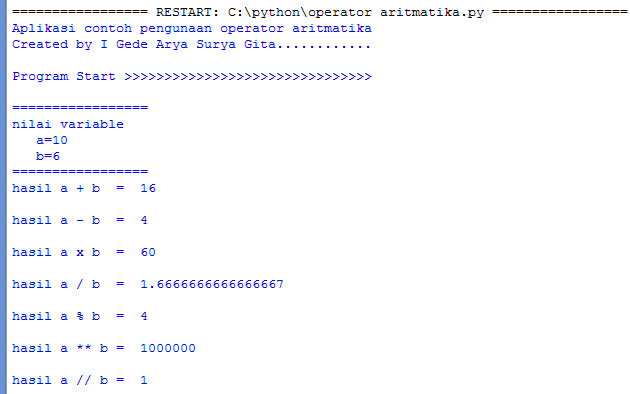
\includegraphics[width=0.25\textwidth]{figures/ctharitmatika}}
 	\caption{Contoh Operator Aritmatika}
 	\label{contoh}
\end{figure}

\vspace{12pt}
\noindent
Bahasa Python mendukung jenis operator berikut. \par
\vspace{12pt}
\noindent
\begin{enumerate}
	\item Operator Aritmatika
	\item Operator Perbandingan (Relasional)
	\item Operator Penugasan \par
	\item Operator Logis \par
	\item Bitwise Operator \par
	\item Operator keanggotaan \par
	\item Operator Identitas \par
\end{enumerate}


Mari kita lihat semua operator sebagai berikut. \par
\vspace{12pt}
\noindent
Operator Aritmatika Python \par
\vspace{12pt}
\noindent
Asumsikan variabel a memiliki 10 dan variabel b memiliki 20, maka  \par
\vspace{12pt}
\noindent
+ Tambahan \par
\noindent
Menambahkan nilai dari kedua sisi operator. \par
\noindent
Contoh A + b = 30 \par
\vspace{12pt}
\noindent
- Pengurangan \par
\noindent
Kurangi operan tangan kanan dari operan tangan kiri. \par
\noindent
Contoh a - b = -10 \par
\vspace{12pt}
\noindent
* Perkalian \par
\noindent
Kalikan nilai di kedua sisi operator \par
\noindent
Contoh a * b = 200 \par
\vspace{12pt}
\noindent
/ Divisi \par
\noindent
Membagi operan tangan kiri dengan tangan kanan operan \par
\noindent
Contoh B / a = 2 \par
\vspace{12pt}
\noindent
 $  \%  $ Modulus \par
\noindent
Membagi operan tangan kiri dengan operan tangan kanan dan mengembalikan sisa \par
\noindent
Contoh B $  \%  $ a = 0 \par
\vspace{12pt}
\noindent
** Eksponen \par
\noindent
Melakukan perhitungan eksponensial (daya) pada operator \par
\noindent
Contoh A ** b = 10 ke daya 20 \par
\vspace{12pt}
\noindent
// \par
\vspace{12pt}
\noindent
Divisi Lantai - Pembagian operan dimana hasilnya adalah hasil bagi di mana angka setelah titik desimal dikeluarkan. $  $Tapi jika salah satu operan negatif, hasilnya berlantai, yaitu terbulatkan dari nol (menuju negatif tak terbatas): \par
\vspace{12pt}
\noindent
9 // 2 = 4 dan 9.0 // 2.0 = 4.0, -11 // 3 = -4, -11.0 // 3 = -4.0 \par
\vspace{12pt}
\noindent
Operator Perbandingan Python \par
\vspace{12pt}
\noindent
Operator ini membandingkan nilai di kedua sisi dan memutuskan hubungan di antara keduanya. $  $Mereka juga disebut operator relasional. \par
\vspace{12pt}
\noindent
Asumsikan variabel a memegang 10 dan variabel b memegang 20, maka  \par
\vspace{12pt}
\noindent
== \par
\noindent
Jika nilai dua operan sama, maka kondisinya menjadi benar. \par
\noindent
Contoh (a == b) tidak benar \par
\vspace{12pt}
\noindent
! = \par
\noindent
Jika nilai dua operan tidak sama, maka kondisinya menjadi benar. \par
\vspace{12pt}
\noindent
> \par
\noindent
Jika nilai operan kiri lebih besar dari nilai operan kanan, maka kondisinya menjadi benar. \par
\noindent
Contoh (a> b) tidak benar \par
\vspace{12pt}
\noindent
< \par
\noindent
Jika nilai operan kiri kurang dari nilai operan kanan, maka kondisinya menjadi benar. \par
\noindent
Contoh (A <b) adalah benar. \par
\vspace{12pt}
\noindent
> = \par
\noindent
Jika nilai operan kiri lebih besar dari atau sama dengan nilai operan kanan, maka kondisinya menjadi benar. \par
\noindent
Contoh (a> = b) tidak benar \par
\vspace{12pt}
\noindent
<= \par
\noindent
Jika nilai operan kiri kurang dari atau sama dengan nilai operan kanan, maka kondisinya menjadi benar. \par
\noindent
Contoh (a <= b) adalah benar. \par
\vspace{12pt}
\noindent
Operator Penugasan Python \par
\vspace{12pt}
\noindent
Asumsikan variabel a memegang 10 dan variabel b memegang 20, maka - \par
\vspace{12pt}
\noindent
= \par
\noindent
Menetapkan nilai dari operan sisi kanan ke operan sisi kiri \hspace*{4.41in}  \par
\noindent
Contoh : c = a + b memberi nilai a + b ke c \par
\noindent
\vspace{12pt}
\noindent
+ = Tambahkan DAN \par
\noindent
Ini menambahkan operan kanan ke operan kiri dan menetapkan hasilnya ke operan kiri \par
\noindent
Contoh : c + = a setara dengan c = c + a \par
\noindent
\vspace{12pt}
\noindent
- = Kurangi DAN \par
\noindent
Ini mengurangi opera kanan dari operan kiri dan menetapkan hasilnya ke operan kiri \par
\noindent
Contoh : c - = a setara dengan c = c – a \par
\noindent
\vspace{12pt}
\noindent
* = Multiply DAN \par
\noindent
Ini mengalikan operan kanan dengan operan kiri dan menetapkan hasilnya ke operan kiri \par
\noindent
Contoh : c * = a setara dengan c = c * a \par
\noindent
\vspace{12pt}
\noindent
/ = Bagilah dan \par
\noindent
Ini membagi operan kiri dengan operan kanan dan menetapkan hasilnya ke operan kiri \par
\noindent
Contoh : C / = a adalah setara dengan c = c / ac / = a adalah setara dengan c = c / a \par
\noindent
\vspace{12pt}
\noindent
 $  \%  $ = Modulus DAN \par
\noindent
Dibutuhkan modulus menggunakan dua operan dan menetapkan hasilnya ke operan kiri \par
\noindent
Contoh : C $  \%  $ = a setara dengan c = c $  \%  $ a \par
\noindent
\vspace{12pt}
\noindent
** = Eksponen DAN \par
\noindent
Melakukan perhitungan eksponensial (daya) pada operator dan memberikan nilai pada operan kiri \par
\noindent
Contoh : C ** = a setara dengan c = c ** a \par
\noindent
\vspace{12pt}
\noindent
// Divisi Lantai \par
\noindent
Ini melakukan pembagian lantai pada operator dan memberikan nilai ke operan kiri \par
\noindent
Contoh : C // = a sama dengan c = c // a \par
\noindent
\vspace{12pt}
\noindent
Operator Bitwise Python \par
\vspace{12pt}
\noindent
Operator Bitwise bekerja pada bit dan melakukan operasi bit by bit. $  $Asumsikan jika a = 60; $  $Dan b = 13; $  $Sekarang dalam format biner mereka akan menjadi seperti berikut - \par

\begin{verbatim}
a = 0011 1100
b = 0000 1101
a & b = 0000 1100
A | b = 0011 1101
a ^ b = 0011 0001
~ a = 1100 0011
\end{verbatim}

Ada beberapa operator Bitwise berikut yang didukung oleh bahasa Python \par
\vspace{12pt}
\noindent
 $  \&  $ Biner DAN \par
\noindent
Operator menyalin sedikit ke hasil jika ada di kedua operan \par
\noindent
Contoh : (A  $  \&  $ b) (berarti 0000 1100) \par
\vspace{12pt}
\noindent
 $  \vert  $ $  $Biner ATAU \par
\noindent
Ini salinan sedikit jika ada di salah satu operan. \par
\noindent
Contoh : (A  $  \vert  $ b) = 61 (berarti 0011 1101) \par
\vspace{12pt}
\noindent
 $  \string^  $ Biner XOR \par
\noindent
Ini salinan bit jika diatur dalam satu operand tapi tidak keduanya. \par
\noindent
Contoh : (A  $  \string^  $ b) = 49 (berarti 0011 0001) \par
\vspace{12pt}
\noindent
 $  \sim  $ Binary Ones Complement \par
\noindent
Ini tidak mencolok dan memiliki efek bit 'flipping'. \par
\noindent
Contoh : ( $  \sim  $ A) = -61 (berarti bentuk pelengkap 1100 0011 dalam 2 karena nomor biner yang ditandatangani \par
\vspace{12pt}
\noindent
<< Pergeseran Kiri Biner \par
\noindent
Nilai operan kiri dipindahkan ke kiri oleh jumlah bit yang ditentukan oleh operan kanan. \par
\noindent
Contoh : Sebuah << = 240 (berarti 1111 0000) \par
\vspace{12pt}
\noindent
>> Binary Right Shift \par
\noindent
Nilai operan kiri dipindahkan tepat dengan jumlah bit yang ditentukan oleh operan kanan. \par
\noindent
Contoh : a >> = 15 (berarti 0000 1111) \par
\vspace{12pt}
\noindent
Operator Logika Python \par
\vspace{12pt}
\noindent
Ada beberapa operator logis berikut yang didukung oleh bahasa Python. $  $Asumsikan variabel a memegang 10 dan variabel b memegang 20 kemudian \par
\vspace{12pt}
\noindent
Digunakan untuk membalik keadaan logis operannya. \par
\vspace{12pt}
\noindent
Keanggotaan Python Operator \par
\vspace{12pt}
\noindent
Operator keanggotaan Python menguji keanggotaan secara berurutan, seperti senar, daftar, atau tupel. $  $Ada dua operator keanggotaan seperti yang dijelaskan di bawah ini \par
\vspace{12pt}
\noindent
Di \par
\noindent
Mengevaluasi ke true jika menemukan sebuah variabel dalam urutan yang ditentukan dan false sebaliknya. \par
\noindent
Contoh : X di y, di sini menghasilkan 1 jika x adalah anggota dari urutan y. \par
\vspace{12pt}
\noindent
tidak masuk \par
\noindent
Mengevaluasi ke true jika tidak menemukan variabel dalam urutan yang ditentukan dan false sebaliknya. \par
\noindent
Contoh : X tidak di y, di sini tidak menghasilkan 1 jika x bukan anggota urutan y. \par
\vspace{12pt}
\noindent
Operator Identitas Python \par
\vspace{12pt}
\noindent
Operator identitas membandingkan lokasi memori dari dua objek. $  $Ada dua operator Identitas yang dijelaskan di bawah ini: \par
\vspace{12pt}
\noindent
aku s \par
\noindent
Mengevaluasi ke true jika variabel di kedua sisi operator menunjuk ke objek yang sama dan salah sebaliknya. \par
\noindent
Contoh: X adalah y, di sini $  $adalah $  $hasil dalam 1 jika id (x) sama dengan id (y). \par
\vspace{12pt}
\noindent
Tidak \par
\noindent
Mengevaluasi false jika variabel di kedua sisi operator menunjuk ke objek yang sama dan benar sebaliknya. \par
\noindent
Contoh: X bukan y, $  $ini bukan $  $hasil 1 jika id (x) tidak sama dengan id (y). \par
\vspace{12pt}
\noindent
Operator Python Diutamakan \par
\vspace{12pt}
\noindent
 berikut mencantumkan semua operator dari preseden tertinggi sampai yang terendah. \par
\vspace{12pt}
\noindent
** \par
\noindent
Eksponensiasi (naik ke tampuk kekuasaan) \par
\vspace{12pt}
\noindent
 $  \sim  $ + - \par
\noindent
Pelengkapan, unary plus dan minus (nama metode untuk dua yang terakhir adalah + @ dan - @) \par
\vspace{12pt}
\noindent
* / $  \%  $ // \par
\noindent
Kalikan, bagi, modulo dan pembagian lantai \par
\vspace{12pt}
\noindent
+ - \par
\noindent
Penambahan dan pengurangan \par
\vspace{12pt}
\noindent
>> << \par
\noindent
Pergeseran bitwise kanan dan kiri \par
\vspace{12pt}
\noindent
 $  \&  $ \par
\noindent
Bitwise 'DAN' \par
\vspace{12pt}
\noindent
 $  \string^  $  $  \vert  $ \par
\noindent
Bitwise eksklusif `OR 'dan reguler` OR' \par
\vspace{12pt}
\noindent
<= <>> = \par
\noindent
Operator perbandingan \par
\vspace{12pt}
\noindent
<> ==! = \par
\noindent
Operator kesetaraan \par
\vspace{12pt}
\noindent
= $  \%  $ = / = // = - = + = * = ** = \par
\noindent
Operator penugasan \par
\vspace{12pt}
\noindent
Bukan \par
\noindent
Operator identitas \par
\vspace{12pt}
\noindent
Bukan di \par
\noindent
Operator keanggotaan \par
\vspace{12pt}
\noindent
Tidak atau dan \par
\noindent
Operator logika \par
\vspace{12pt}
\noindent
Peran operator dalam proses perhitungan matematika sangatlah penting. Selain $  $operator Aritmatika, Python juga mendukung $  $operator berkondisi $  $yang berfungsi untuk membandingkan suatu nilai dengan nilai yang lain. Operator-operator yang didukung oleh Python yaitu $  $operator Unari $  $( + dan – ) dan $  $operator Binari $  $( +, -, *, /,  $  \%  $, dan **). Pada ekspresi Aritmatika berikut:\vspace{\baselineskip}
\vspace{\baselineskip}
x = y + z \par
\noindent
y $  $dan $  $z $  $disebut sebagai operan dari operator $  $+. Tabel di bawah ini menjelaskan tentang berbagai macam operator yang digunakan untuk segala perhitungan di Python. \par
\vspace{12pt}
\noindent
Jika sebuah ekspresi melibatkan lebih dari satu operator, Python secara otomatis akan memilih operator mana yang akan diutamakan dahulu. Sebagai contoh: \par
\begin{verbatim}
>>> x=7+3*6
>>> x
25
>>> y=100/4*5
>>> y
125

\end{verbatim}
Operator $  $** $  $memiliki urutan tertinggi diantara operator lainnya. Operator $  $* $  $mempunyai urutan lebih tinggi daripada operator $  $+, dan operator $  $/ $  $mempunyai urutan yang sama dengan operator $  $*. Pada ekspresi $  $x = 7 + 3 * 6, bagian $  $3 * 6 $  $akan dieksekusi pertama kali menghasilkan $  $18, yang kemudian ditambahkan dengan $  $7. Sedangkan ekspresi $  $y = 100/4*5, bagian $  $100/4dieksekusi terlebih dahulu karena operator $  $/ $  $berada disebelah kiri dari operator $  $*. \par
\vspace{12pt}
\noindent
Kita bisa mengubah urutan prioritas dari operator Aritmatika dengan menggunakan kurung-buka-kurung-tutup $  $(). Operator $  $() $  $memiliki urutan tertinggi diantara tiga tipe lainnya. Operator $  $() $  $mempunyai urutan dari kiri ke kanan pada ekspresi di dalamnya. Berikut ini contohnya: \par
\vspace{12pt}
\noindent
>>> x=(7+3)*6\vspace{\baselineskip}
>>> x\vspace{\baselineskip}
60\vspace{\baselineskip}
>>> y=100/(4*5)\vspace{\baselineskip}
>>> y\vspace{\baselineskip}
5\vspace{\baselineskip}
>>> z=7+(5*(8/2)+(4+6))\vspace{\baselineskip}
>>> z\vspace{\baselineskip}
37 \par
\vspace{12pt}
\noindent
Operator modulus $  $ $  \%  $ $  $akan memberikan nilai sisa dari pembagian integer. Berikut contoh penggunaan operator modulus: \par
\vspace{12pt}
\noindent
>>> 7  $  \%  $ 3\vspace{\baselineskip}
1\vspace{\baselineskip}
>>> 0  $  \%  $ 3\vspace{\baselineskip}
0\vspace{\baselineskip}
>>> 1.0  $  \%  $ 3.0\vspace{\baselineskip}
1.0 \par
\vspace{12pt}
\noindent
Operator eksponensial $  $akan memberikan nilai pangkat dari suatu bilangan. Contoh penggunaan operator eksponensial: \par
\vspace{12pt}
\noindent
>>> 5**2\vspace{\baselineskip}
25\vspace{\baselineskip}
>>> 5**-2\vspace{\baselineskip}
0.04\vspace{\baselineskip}
>>> -5**2\vspace{\baselineskip}
-25\vspace{\baselineskip}
>>> (-5)**2\vspace{\baselineskip}
25 \par
\vspace{12pt}
\noindent
Operator Penugasan Python \par
\vspace{12pt}
\noindent
Asumsikan variabel a memiliki 10 dan variabel b memiliki 20, maka - \par
\vspace{12pt}
\noindent
= \par
\noindent
Menetapkan nilai dari operan sisi kanan ke operan sisi kiri \hspace*{4.41in}  \par
\noindent
Contoh : c = a + b memberi nilai a + b ke c \par
\noindent
\vspace{12pt}
\noindent
+ = Tambahkan DAN \par
\noindent
Ini menambahkan operan kanan ke operan kiri dan menetapkan hasilnya ke operan kiri \par
\noindent
Contoh : c + = a setara dengan c = c + a \par
\noindent
\vspace{12pt}
\noindent
- = Kurangi DAN \par
\noindent
Ini mengurangi opera kanan dari operan kiri dan menetapkan hasilnya ke operan kiri \par
\noindent
Contoh : c - = a setara dengan c = c – a \par
\noindent
\vspace{12pt}
\noindent
* = Multiply DAN \par
\noindent
Ini mengalikan operand kanan dengan operan kiri dan menetapkan hasilnya ke operan kiri \par
\noindent
Contoh : c * = a setara dengan c = c * a \par
\noindent
\vspace{12pt}
\noindent
/ = Bagilah dan \par
\noindent
Ini membagi operan kiri dengan operan kanan dan menetapkan hasilnya ke operan kiri \par
\noindent
Contoh : C / = a adalah setara dengan c = c / ac / = a adalah setara dengan c = c / a \par
\noindent
\vspace{12pt}
\noindent
 $  \%  $ = Modulus DAN \par
\noindent
Dibutuhkan modulus menggunakan dua operan dan menetapkan hasilnya ke operan kiri \par
\noindent
Contoh : C $  \%  $ = a setara dengan c = c $  \%  $ a \par
\noindent
\vspace{12pt}
\noindent
** = Eksponen DAN \par
\noindent
Melakukan perhitungan eksponensial (daya) pada operator dan memberikan nilai pada operan kiri \par
\noindent
Contoh : C ** = a setara dengan c = c ** a \par
\noindent
\vspace{12pt}
\noindent
// Divisi Lantai \par
\noindent
Ini melakukan pembagian lantai pada operator dan memberikan nilai ke operan kiri \par
\noindent
Contoh : C // = a sama dengan c = c // a \par
\noindent
\vspace{12pt}
\noindent
Operator Bitwise Python \par
\vspace{12pt}
\noindent
Operator Bitwise bekerja pada bit dan melakukan operasi bit dari bit. $  $Asumsikan jika a = 60; $  $Dan b = 13; $  $Sekarang dalam format biner mereka akan menjadi seperti berikut - \par
\vspace{12pt}
\noindent
a = 0011 1100 \par
\vspace{12pt}
\noindent
b = 0000 1101 \par
\vspace{12pt}
\vspace{12pt}
\noindent
a  $  \&  $ b = 0000 1100 \par
\vspace{12pt}
\noindent
A  $  \vert  $ b = 0011 1101 \par
\vspace{12pt}
\noindent
a  $  \string^  $ b = 0011 0001 \par
\vspace{12pt}
\noindent
 $  \sim  $ a = 1100 0011 \par
\vspace{12pt}
\noindent
Ada beberapa operator Bitwise berikut yang didukung oleh bahasa Python \par
\vspace{12pt}
\noindent
 $  \&  $ Biner DAN \par
\noindent
Operator menyalin sedikit ke hasil jika ada di kedua operan \par
\noindent
Contoh : (A  $  \&  $ b) (berarti 0000 1100) \par
\vspace{12pt}
\noindent
 $  \vert  $ $  $Biner ATAU \par
\noindent
Ini salinan sedikit jika ada di salah satu operan. \par
\noindent
Contoh : (A  $  \vert  $ b) = 61 (berarti 0011 1101) \par
\vspace{12pt}
\noindent
 $  \string^  $ Biner XOR \par
\noindent
Ini salinan bit jika diatur dalam satu operand tapi tidak keduanya. \par
\noindent
Contoh : (A  $  \string^  $ b) = 49 (berarti 0011 0001) \par
\vspace{12pt}
\noindent
 $  \sim  $ Binary Ones Complement \par
\noindent
Ini tidak mencolok dan memiliki efek bit 'flipping'. \par
\noindent
Contoh : ( $  \sim  $ A) = -61 (berarti bentuk pelengkap 1100 0011 dalam 2 karena nomor biner yang ditandatangani \par
\vspace{12pt}
\noindent
<< Pergeseran Kiri Biner \par
\noindent
Nilai operan kiri dipindahkan ke kiri oleh jumlah bit yang ditentukan oleh operan kanan. \par
\noindent
Contoh : Sebuah << = 240 (berarti 1111 0000) \par
\vspace{12pt}
\noindent
>> Binary Right Shift \par
\noindent
Nilai operan kiri dipindahkan tepat dengan jumlah bit yang ditentukan oleh operan kanan. \par
\noindent
Contoh : a >> = 15 (berarti 0000 1111) \par
\vspace{12pt}
\noindent
Operator Perbandingan Python \par
\vspace{12pt}
\noindent
Operator ini membandingkan nilai di kedua sisi dan memutuskan hubungan di antara keduanya. $  $Mereka juga disebut operator relasional. \par
\vspace{12pt}
\noindent
Asumsikan variabel a memegang 10 dan variabel b memegang 20, maka  \par
\vspace{12pt}
\noindent
== \par
\noindent
Jika nilai dua operan sama, maka kondisinya menjadi benar. \par
\noindent
Contoh (a == b) tidak benar \par
\vspace{12pt}
\noindent
! = \par
\noindent
Jika nilai dua operan tidak sama, maka kondisinya menjadi benar. \par
\vspace{12pt}
\noindent
> \par
\noindent
Jika nilai operan kiri lebih besar dari nilai operan kanan, maka kondisinya menjadi benar. \par
\noindent
Contoh (a> b) tidak benar \par
\vspace{12pt}
\noindent
< \par
\noindent
Jika nilai operan kiri kurang dari nilai operan kanan, maka kondisinya menjadi benar. \par
\noindent
Contoh (A <b) adalah benar. \par
\vspace{12pt}
\noindent
> = \par
\noindent
Jika nilai operan kiri lebih besar dari atau sama dengan nilai operan kanan, maka kondisinya menjadi benar. \par
\noindent
Contoh (a> = b) tidak benar \par
\vspace{12pt}
\noindent
<= \par
\noindent
Jika nilai operan kiri kurang dari atau sama dengan nilai operan kanan, maka kondisinya menjadi benar. \par
\noindent
Contoh (a <= b) adalah benar. \par
\noindent
Operator Python Diutamakan \par
\vspace{12pt}
\noindent
 berikut mencantumkan semua operator dari preseden tertinggi sampai yang terendah. \par
\vspace{12pt}
\noindent
** \par
\noindent
Eksponensiasi (naik ke tampuk kekuasaan) \par
\vspace{12pt}
\noindent
 $  \sim  $ + - \par
\noindent
Pelengkap, unary plus dan minus (nama metode untuk dua yang terakhir adalah + @ dan - @) \par
\vspace{12pt}
\noindent
* / $  \%  $ // \par
\noindent
Kalikan, bagi, modulo dan pembagian lantai \par
\vspace{12pt}
\noindent
+ - \par
\noindent
Penambahan dan pengurangan \par
\vspace{12pt}
\noindent
>> << \par
\noindent
Pergeseran bitwise kanan dan kiri \par
\vspace{12pt}
\noindent
 $  \&  $ \par
\noindent
Bitwise 'DAN' \par
\vspace{12pt}
\noindent
 $  \string^  $  $  \vert  $ \par
\noindent
Bitwise eksklusif `OR 'dan reguler` OR' \par
\vspace{12pt}
\noindent
<= <>> = \par
\noindent
Operator perbandingan \par
\vspace{12pt}
\noindent
<> ==! = \par
\noindent
Operator kesetaraan \par
\vspace{12pt}
\noindent
= $  \%  $ = / = // = - = + = * = ** = \par
\noindent
Operator penugasan \par
\vspace{12pt}
\noindent
Bukan \par
\noindent
Operator identitas \par
\vspace{12pt}
\noindent
Bukan di \par
\noindent
Operator keanggotaan \par
\vspace{12pt}
\noindent
Tidak atau dan \par
\noindent
Operator logika \par
\vspace{12pt}
\vspace{12pt}



\chapter{Desicion Making}
\section{Python Decision Making}
Pengambilan keputusan adalah antisipasi kondisi yang terjadi saat pelaksanaan program dan menentukan tindakan yang dilakukan sesuai kondisi. 
Struktur keputusan mengevaluasi banyak ekspresi yang menghasilkan TRUE atau FALSE sebagai hasil.   Anda perlu menentukan tindakan mana yang harus diambil dan pernyataan mana yang akan dijalankan jika hasilnya BENAR atau SALAH sebaliknya. 
Berikut adalah bentuk umum dari struktur pengambilan keputusan yang khas atau khusus yang ditemukan di sebagian besar bahasa pemrograman
\ref{diagramstruktur}.
\begin{figure}[ht]
    \centerline{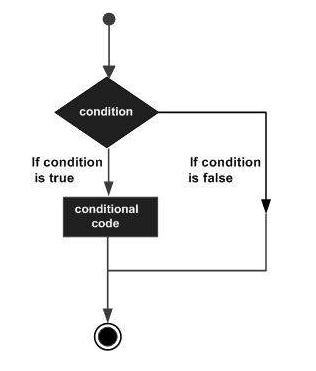
\includegraphics[width=0.25\textwidth]{figures/struktur}}
    \caption{struktur pada python}
    \label{diagramstruktur}
    \end{figure}
Bahasa pemrograman Python menyediakan jenis dan juga laporan pengambilan keputusan. Berikut ini adalah penjelasan tentang pernyataan dan deskripsinya :
\begin{enumerate}
\item
if statements : sebuah if statement terdiri dari ekspresi boolean diikuti oleh satu atau lebih pernyataan. 
\item
if...else statements : sebuah if statement dapat diikuti oleh opsinal else statement, yang mengeksekusi ketika ekspresi boolean adalah palsu. 
\item
nested if statements : anda dapat menggunakan satu if atau else if pernyataan di dalam lain if atau else if statements. 
\end{enumerate}
Decision making atau Pemilihan keputusan pada python sangat penting untuk pemrograman komputer. Akan ada banyak situasi saat Anda diberi dua pilihan atau lebih dan Anda harus memilih opsi berdasarkan kondisi yang diberikan. Misalnya,
\begin{enumerate} 
\item
Seorang murid dengan nilai lebih dari 90 disebut siswa pintar 
\item
Seorang murid dengan nilai dibawah 90 dan diatas 30 disebut Siswa Standard 
\item
Seorang murid dengan nilai dibawah 30 disebut siswa bodoh 
\end{enumerate}

Umumnya juga, decision making dalam bahasa pemrograman yang sering digunakan adalah :
\begin{enumerate}
\item
if...else statement : berguna saat kita harus mengambil keputusan dari dua pilihan. Misalnya, jika seorang siswa mendapatkan nilai lebih dari angka 95, maka siswa itu pintar, jika tidak, situasi seperti itu dapat dikodekan. 
\item
if...elseif...else statement : merupakan optional dari if...else statement, yang sangat berguna untuk menentukan berbagai kondisi yang lebih dari 2. 
\item
switch statement : merupakan alternative dari if statement. Setiap nilai disebut case, dan variabel yang dicek untuk setiap switch case. 
\end{enumerate}

F...ELIF...ELSE statement sama seperti IF...ELSEIF...ELSE pada bahasa pemrograman Java, yaitu digunakan menyeleksi beberapa ekspresi (lebih dari satu), apabila eskpresi1 pertama bernilai true, maka akan dijalankan statement1, jika ekspresi2 kedua bernilai true, maka akan dijalankan statement2, dan seterusnya.

Dari contoh diatas, pertanyaannya adalah bagaimana cara menulis kode pemrograman untuk menangani situasi seperti itu. Hampir semua bahasa pemrograman memberikan pernyataan kondisional diatas berdasarkan diagram decision di bawah. 
\begin{figure}[ht]
	    \centerline{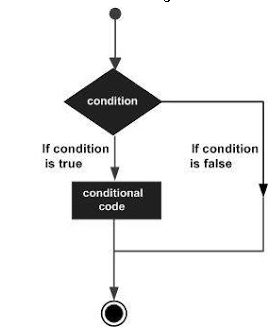
\includegraphics[width=0.25\textwidth]{figures/diagram_decision}}
	    \caption{diagram decision}
	    \label{diagramdecisionmaking}
	    \end{figure} 

Mari kita membuat sebuah program C dengan bantuan jika pernyataan kondisional untuk mengubah situasi yang diberikan di atas menjadi kode pemrograman:  
\begin{verbatim}
#include <stdio.h>
 
main() {
   int x = 45;
   if( x > 95) {
      printf( "siswa pintar");
   }
   if( x < 30) {
      printf( "siswa bodoh");
   }
   if( x < 95 && x > 30 ) {
      printf( "Siswa Standard");
   }
}
\end{verbatim}
Outputnya adalah Siswa Standard

Bahasa pemrograman Python mengasumsikan nilai   non-nol   dan   non-nullsebagai TRUE, dan jika itu adalah   nol   atau   nol   , maka diasumsikan sebagai nilai FALSE. 
Bahasa pemrograman Python menyediakan jenis pernyataan pengambilan keputusan berikut. 

 
Mari kita membahas setiap keputusan secara singkat  

 
Setelah tutorial mengenai  
\subsection{variable dan operator}
pada bahasa pemrograman python akan membahas mengenai percabangan/pengambilan keputusan. Percabangan atau pengambilan keputusan adalah pengkondisian yang terjadi ketika aplikasi berjalan, kemudian ada aksi-aksi tertentu atau kondisi tertentu sehingga aplikasi harus bereaksi terhadap hal itu. Atau dalam bahasa pemrograman umum dikenal dengan IF, THEN, ELSE sebagai contoh pengaplikasian dari pengambilan keputusan ini. 

if statements
Sebuah if statement terdiri dari ekspresi boolean diikuti oleh satu atau lebih pernyataan.
 
Pada pembahasan python decisiom makaing ini, kami menggunakan perangkat raspberry pi 2 dengan sistem operasi rasbian jessie. Sangat ringan dan tentunya python secara default ada di dalamnya. Kebetulan dalam tulisan ini masih menggunakan python versi 2, meskipun ada python versi 3 juga. 

 
Python core tidak menyediakan   \" switch  \"  atau   " case  \"  seperti bahasa pemrograman lain. Tapi kita bisa menggunakan statemen if, elif yang bisa menggantikan   \" switch  \"  atau   \" case  \" . 

 
Di bawah ini merupakan tipe-tipe percabangan yang disediakan oleh python. 

 
IF : Mengandung ekspresi boolean dan diikuti oleh satu atau banyak statemen 

 
IF ELSE : IF bisa diikuti oleh optional statemen yaitu ELSE, yang akan dieksekusi ketika ekspresi boolean bernilai FALSE 

 
NESTED IF atau IF bersarang :~ Kita bisa menggunakan IF, ELSE IF di dalam IF, ELSE IF lainnya 

 
Contoh dalam python untuk IF :  

 
varAngka1 = 123 

 
varAngka2 = 0 

 
if varAngka1: 

 
                                               print "Nilai : TRUE" 

 
                                                print varAngka1 

 
if varAngka2: 

 
                                               print "Nilai : TRUE" 

 
print varAngka2{\fontsize{14pt}{14pt}\selectfont     \\} 

 
\begin{verbatim}
#/usr/bin/python
a = raw_input("Masukkan Angka = ")
b = int(a)
if (b%2==0):
        print "Genap"
else:
        print "Ganjil"
\end{verbatim}

Contoh untuk IF ELIF ELSE, di python sintak ini bisa ditulis dengan lebih singkat yaitu elif :  

 
varAngka = 123 
 
    
 
if varAngka==200: 

 
                           print "Nilai : TRUE" 

 
                           print varAngka 

 
elif varAngka==123: 

 
                           print "Nilai : TRUE" 

 
                           print varAngka 

 
else: 

 
                           print "Nilai : FALSE" 

 
                           print varAngka 

 
Contoh untuk NESTED IF :  

\begin{verbatim}
varAngka = 89 
 
    
 
if varAngka<100: 

 
                       print \"Nilai : TRUE\" 

 
                       print varAngka 

 
                       if varAngka > 80: 

 
                                                print \"Nilai : A\" 

 
                       elif varAngka > 60: 

 
                                                print \"Nilai : B\" 

 
                       elif varAngka > 40: 

 
                                              print \"Nilai : C\" 

 
                       elif varAngka > 20: 

 
                                             print \"Nilai : D\" 

 
                        $else: 

 
                                            \ print \"Nilai : E\" 

 
else: 

                        print \"Nilai : FALSE\" 

 
                        print varAngka 
  end{verbatim}


Contoh lain pada NESTED IF dengan kondisi pilihan lebih dari satu. Seperti menentukan game yang sangat disukai : 
\vspace{12}
 
Begin{verbatim}
#/usr/bin/python
pilihan=2
if pilihan==1:
        print "DOTA 2"
else:
        if pilihan==2:
		print "GTA V Online"
	else:
		print "Semua Game"
end{verbatim}

Perintah seperti diatas itu adalah NESTED IF yaitu terdapat IF di dalam IF. 

 
Statemen IF juga bisa ditulis dalam 1 baris saja, misalnya seperti ini :  

 
if varAngka1: print \"Nilai : TRUE\" 

 
Dari sintak percabangan sudah bisa kita lihat perbedaan di antara python dengan menggunakan bahasa pemrograman yang lain. Sintak ditulis dengan lebih ringkas dibanding dengan yang lain. Percabangan atau pengkondisian ini adalah hal dasar dalam pemrograman pada umumnya, kita pasti akan menggunakannya. Pada tulisan yang akan dibuat selanjutnya saya akan menulis mengenai perulangan atau looping dalam python. 

 
Suite pernyataan tunggal 

 
Jika rangkaian   klausa   jika   hanya terdiri dari satu baris, itu mungkin sama pada baris perintah sebagai pernyataan header. 

 
Berikut adalah contoh   klausa   satu baris jika   - 


 
var = 100 

 
if ( var~ == 100 ) : print "Value of expression is 100" 

 
print "Good bye!" 

 
Bila kode diatas dieksekusi, maka menghasilkan hasil sebagai berikut - 

 
Value of expression is 100 

 
Good bye! \hspace*{1.31in}  
 

 
Pengambilan keputusan (kondisi if) digunakan untuk mengantisipasi kondisi yang terjadi saat jalanya program dan menentukan tindakan apa yang akan diambil sesuai dengan kondisi. 
 

 
Pada python ada beberapa statement atau kondisi diantaranya adalah   if,   else   dan   elif   Kondisi   if   digunakan untuk mengeksekusi kode jika kondisi bernilai benar. 
 

 
Jika kondisi bernilai salah maka statement atau kondisi if tidak akan di-eksekusi. 
 

Dibawah ini adalah contoh penggunaan kondisi if pada Python 
 

Dari contoh diatas, jika program dijalankan maka akan mencetak string \"Selamat Anda Lulus Ujian\" sebanyak 1 kali yaitu pada if pertama. Di if kedua statement bernilai salah, jadi perintah   print(\"Selamat Anda Lulus\")   tidak akan dieksekusi. 
 

Selanjutnya Anda bisa mempelajari kondisi if else 

 
Pengambilan keputusan (kondisi if else) tidak hanya digunakan untuk menentukan tindakan apa yang akan diambil sesuai dengan kondisi, tetapi juga digunakan untuk menentukan tindakan apa yang akan diambil atau dijalankan jika kondisi tidak sesuai.

 
 
Pada python ada beberapa statement atau kondisi diantaranya adalah   if,   else   dan   elif   Kondisi   if   digunakan untuk mengeksekusi kode jika kondisi bernilai benar.

 
 
Kondisi if else adalah kondisi dimana jika pernyataan benar (true) maka kode dalam if akan dieksekusi, tetapi jika bernilai salah (false) maka akan mengeksekusi kode di dalam else.

 
 
Dibawah ini adalah contoh penggunaan kondisi if else pada Python 

 
Kondisi if else adalah jika kondisi bernilai TRUE maka akan dieksekusi pada if, tetapi jika bernilai FALSE maka akan dieksekusi kode pada else 
 

nilai = 3
 
 
Jika pernyataan pada if bernilai TRUE maka if akan dieksekusi, tetapi jika FALSE kode pada else yang akan dieksekusi.
 
 
if(nilai > 7):
        
 
 print(\"Selamat Anda Lulus\")
 
 
else:
 
 
        print(\"Maaf Anda Tidak Lulus\") 
 


Pada contoh diatas, jika program dijalankan maka akan mencetak string \"Maaf Anda Tidak Lulus\" karena pernyataan pada if bernilai FALSE 
 

Selanjutnya kita akan mempelajari per-kondisi an pada python yang terakhir yaitu \"Elif\"    

 
Pengambilan keputusan (kondisi if elif) merupakan lanjutan atau percabangan logika dari \"kondisi if\". Dengan elif kita bisa membuat kode program yang akan menyeleksi beberapa kemungkinan yang bisa terjadi. Hampir sama dengan kondisi \"else\", bedanya kondisi \"elif\" bisa banyak dan tidak hanya satu.   

Dibawah ini adalah contoh penggunaan kondisi elif pada Python 

 
Contoh penggunaan kondisi elif 

 
hari   \_  ini = \"Minggu\" 
 


if(hari   \_  ini == \"Senin\"): 
 

        print(\"Saya akan kuliah\") 
 

elif(hari   \_  ini == \"Selasa\"): 
 

        print(\"Saya akan kuliah\") 
 

elif(hari   \_  ini == \"Rabu\"): 
 

        print(\"Saya akan kuliah\") 
 

elif(hari   \_  ini == \"Kamis\"): 
 

        print(\"Saya akan kuliah\") 
 

elif(hari   \_  ini == \"Jumat\"): 
 

 $  $  $  $ print("Saya akan kuliah") 
 

elif(hari $  \_  $ini == "Sabtu"): 
 

 $  $  $  $ print("Saya akan kuliah") 
 

elif(hari $  \_  $ini == "Minggu"): 
 

 $  $  $  $ print("Saya akan libur") 
 


Pada contoh diatas, jika program dijalankan maka akan mencetak   
\"Saya akan libur\". 
 
    Pernyataan tersebut digunakan untuk pengambilan keputusan dalam python berupa if, pernyataan tersebut memiliki format lengkap  yang dapat dilihat sebagai berikut : 

 
\begin{enumerate}
\item
if kondisi   \_  1: 

 
~~~~~~ pernyataan   \_  pernyataan   \_  1 

 
\item
elif kondisi   \_  2: 

 
~~~~~~ pernyataan   \_  pernyataan   \_  2 

 
\item
elif kondisi   \_  3: 

 
~~~~~~ pernyataan   \_  pernyataan   \_  3 

 
\item
else kondisi   \_  n: 

 
~~~~~~ pernyataan   \_  pernyataan-n 

 
~~~~~~  
 
\item
if kondisi   \_  1,elif kondisi   \_  2,elif kondisi   \_  3,else kondisi   \_  n 

 
~~~~berupa~suatu ekspresi yang menghasilkan nilai logika (benar atau salah)    
 
~~~  
\end{enumerated}
 
Contoh Code yang dijalankan pada modus interaktif 


\begin{verbatim}
  x = 5 

 
~ y = 100 

 
~~~ terbesar = x 

 
~~ if terbesar < y: 

 
terbesar = y 

~~~ terbesar = 100  

\end{verbatim}
 
~~~  

 
  Python tidak menggunakan  \{   \}  untuk menyertakan blok kode untuk penggunaan if or loop or fungsi yang lainnya. Sebaliknya, python menggunakan titik dua (:) dan indentasi atau spasi untuk pernyataan  kelompok. Tes  boolean untuk if tidak perlu dalam tanda kurung (perbedaan besar dari C++ atau Java), dan dapat memiliki *elif* dan *else*. 
 

            Nilai apapun dapat digunakan sebagai if-test.
			pada   \" nol  \"  nilai-nilai semua dihitung sebagai false:Tidak ada,0,string kosong,list kosong, dictionary kosong.
			Ada juga tipe Boolean dengan dua nilai: True dan False (jika dikonversi ke int, ini adalah 1 dan 0). 
			Python memiliki operasi perbandingan yang biasa: \verb| ==, =, <, <=,>,> =| 
			Tidak seperti Java dan C.Operator boolean bisa juga di eja seperti * and *, * or *, * not * (Python tidak menggunakan gaya C). 

 
~~~~matakuliah = 'matematika'   matematika,fisika 
 
~~  
 
 nilai = 70 100,80,50 

 
~~~ if nilai >=100 or nilai>=80 : 

 
~~~~~~ if matakuliah == 'matematika': 

 
~~~~~~~~~ print 'anda mendapat nilai A dalam mata kuliah matematika' 

 
~~~ elif matakuliah == 'fisika': 

 
~~~~~~ print 'anda mendapat nilai A dalam mata kuliah Fisika' 

 
~~~ elif nilai >=70 and matakuliah=='matematika': 


 
~~~~~~ print 'anda mendapat nilai B dalam mata kuliah matematika' 

 
~~~ elif nilai >=70 and matakuliah=='fisika': 

 
~~~~~~ print 'anda mendapat nilai B dalam mata kuliah fisika' 

 
~~~ else: 

 
~~~~~~ print 'nilai dan~matakuliah~tidak~ada'~~~     

 
Seperti halnya bahasa pemrograman yang lain, tentu python juga mempunyai perintah untuk pengambilan suatu keputusan terhadap kondisi tertentu, yang disebut percabangan. Percabangan pada bahasa pemrograman python menggunakan perintah if, ya sama dengan bahasa pemrograman yang lain. Bagaimana cara menggunakan perintah if ini dalam bahasa pemrograman python? berikut adaah cara penggunaan percabangan if yang tepat
 

Cara penulisan dari perintah if secara garis besar adalah seperti berikut: 
 


if <kondisi 1>: 
 

   <perintah yang dijalankan 1> 
 

elif <kondisi 2>: 
 

<perintah yang dijalankan 2> 
 

else:
   <perintah yang dijalankan 3> 
 


Perintah-perintah yang dipergunakan antara lain 
 

If dan If bersarang 
 

Elif (singkatan dari: else if) dan 
 

else.
 
 

IF Bersarang 
 

Adapun tanda titik dua diletakan setelah kondisi, sedangkan untuk perintah yang dijalankan jika kondisi if terpenuhi diberi tab atau 4 spasi pada depannya untuk menandakan bahwa perintah tersebut berada didalam if, contoh dalam source code. Misal kita ingin menentukan angka genap atau ganjil: 
 

angka = 7 
 

if angka    \%   2 == 0: 
 

        print 'genap' 
 

else:
   print 'ganjil' 
 

 Dari perintah diatas akan menghasilkan nilai yang diprint adalah 'ganjil'. Tanda  $  \%  $ (persen) disini merupakan operator untuk modulus, yaitu sisa bagi. Adapun jalannya dari program diatas adalah, jika angka dalam hal ini nilainya 7 jika di modulus dengan 2, menyisahkan nilai nol maka data yang diprint adalah genap, jika tidak menyisahkan nilai nol maka data yang diprint adalah ganjil. 
 

Bagaimana halnya dengan kondisi yang lebih dari satu. Misal kita ingin menentukan game yang kita sukai: 
 

pilihan = 2 
 

if pilihan == 1: 
 

        print 'DOTA2' 
 

else:
        if pilihan == 2: 
 

                print 'GTA V Online' 
 

        else: 
 

                print 'Semua Game' 
 

Perintah diatas merupakan if bersarang yaitu terdapat if didalam if, dapat juga dituliskan dengan perintah dibawah ini dengan menggunakan elif: 
 


Elif 
 

Merupakan suatu pemilihan kondisi dimana dalam kondisi tersebut, terdapat lagi kondisi lain
Contoh kodingnya : 
 

Program Kategori Berat hewan qurban 
 

pilihan = 300 
 

if pilihan > 300: 
 

        print 'Sapi boleh diqurban' 
 

elif pilihan <    300 : 
 

        print 'Sapi belum boleh diqurban' 
 

else: 
 

        print ‘Rawat dulu sapinya yang benar' 
 

Mana yang terbaik dari kedua cara penulisan kondisi if yang lebih dari satu diatas itu tentunya sesuai dengan kebutuhan kita masing-masing dalam membuat suatu aplikasi. Dalam if pun kita bisa membuat dua atau lebih persyaratan dalam kondisi if 
 


Else 
 

contohnya:
angka = 2 
 

if angka <= 10 and angka >= 1 : 
 

        print 'angka diantara 1 dan 10' 
 

else: 
 

        print 'angka diluar jangkauan' 

 
Percabangan Pada Bahasa Pemrograman Python. 

 
Seperti halnya bahasa pemrograman yang lain, tentu python juga mempunyai perintah untuk pengambilan suatu keputusan terhadap kondisi tertentu, yang disebut percabangan. Percabangan pada bahasa pemrograman python menggunakan perintah   if, ya sama dengan bahasa pemrograman yang lain. Bagaimana cara menggunakan perintah   if   ini dalam bahasa pemrograman python? Yuk mari kita sama-sama melihat cara penggunaan perintah   if   ini. 

 
Cara penulisan dari perintah if secara garis besar adalah seperti berikut: 
 
if <kondisi 1>: 

 
~~~ <perintah yang dijalankan 1> 

 
elif <kondisi 2>: 

 
~~~ <perintah yang dijalankan 2> 

 
else: 

 
~~~ <perintah yang dijalankan 3> 

 
Perintah-perintah yang dipergunakan antara lain   if,   elif   (singkatan dari:   else if) dan   else. Adapun tanda titik dua diletakan setelah kondisi, sedangkan untuk perintah yang dijalankan jika kondisi if terpenuhi diberi   tab   atau   4 spasi   pada depannya untuk menandakan bahwa perintah tersebut berada didalam if, contoh dalam source code. Misal kita ingin menentukan angka genap atau ganjil: 

 
angka = 7 

 
if angka    \%   2 == 0: 

 
~~~ print 'genap' 

 
else: 

 
~~~ print 'ganjil' 

 
Dari perintah diatas akan menghasilkan nilai yang diprint adalah 'ganjil'. Tanda      \%     (persen) disini merupakan operator untuk modulus, yaitu sisa bagi. Adapun jalannya dari program diatas adalah, jika angka dalam hal ini nilainya 7 jika di modulus dengan 2, menyisahkan nilai nol maka data yang diprint adalah genap, jika tidak menyisahkan nilai nol maka data yang diprint adalah ganjil. 

 
Bagaimana halnya dengan kondisi yang lebih dari satu. Misal kita ingin menentukan buah yang kita sukai: 

 
pilihan = 2 

 
if pilihan == 1: 

 
~~~ print 'buah durian' 

 
else: 

 
~~~ if pilihan == 2: 

 
~~~~~~~ print 'buah mangga' 

 
~~~ else: 

 
~~~~~~~ print 'semua buah' 

 
Perintah diatas merupakan if bersarang yaitu terdapat if didalam if, dapat juga dituliskan dengan perintah dibawah ini dengan menggunakan $  $elif: 

 
pilihan = 2 

 
if pilihan == 1: 

 
~~~ print 'buah durian' 

 
elif pilihan == 2: 

 
~~~ print 'buah mangga' 

 
else: 

 
~~~ print 'semua buah' 

 
Mana yang terbaik dari kedua cara penulisan kondisi if yang lebih dari satu diatas itu tentunya sesuai dengan kebutuhan kita masing-masing dalam membuat suatu aplikasi, seperti kata orang, banyak jalan menuju roma begitu juga dengan pemrograman, banyak jalan untuk menuliskan suatu perintah untuk menghasilkan hasil tertentu... :) 

 
Dalam if pun kita bisa membuat dua atau lebih persyaratan dalam kondisi   if   contohnya: 

 
\begin{verbatim}
angka = 2  
if angka <= 10 and angka >= 1 : 
~~~ print 'angka diantara 1 dan 10' 
else:  
~~~ print 'angka diluar jangkauan' 
\end{verbatim}





\chapter{Loop}
\section{Python Loops}
\begin{figure}[ht]
	\centerline{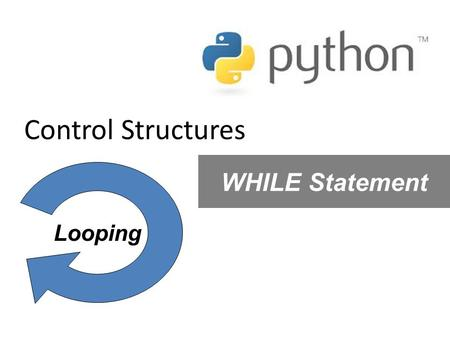
\includegraphics[width=0.25\textwidth]{gambar/perulangan.jpg}}
	\caption{Perulangan}
	\label{perulangan}
\end{figure}
Python dikenal sebagai bahasa pemograman interpreter, karena Python dieksekusi dengan sebuah interpreter. Satu hal yang telah kita ketahui bahwa bahasa pemograman Python adalah bahasa pemograman yang mudah dibaca dan terstruktur. Python sangat mementingkan indentasi, sehingga kita perlu melakukan indentasi secara konsisten. Indentasi tersebut dipermudah dengan penggunaan tombol Tab dan dimulai dari kolom pertama untuk setiap blok baru\cite{santoso2009bahasa}.
Python memiliki kelebihan lain yang sangat penting dibanding bahasa pemrograman yang terdahulu:
\begin{itemize}
\item Python merupakan open-source software, yang artinya ia dapat diperoleh secara gratis. Bahkan python sudah otomatis terinstall di Linux.
\item Python tersedia pada semua operating systems (OS) terkenal seperti Linux, Unix, Windows, dan MacOS. Suatu script python yang ditulis pada OS tertentu, dapat dijalankan di OS lain tapa ada modifikasi sedikitpun.
\item Python lebih mudah dipelajari sekaligus lebih mudah "‘dibaca"’ dibandingkan dengan bahasa pemrograman lainnya.
\item Python dan program ekstensinya mudah diinstall.
\end{itemize}
Python berdiri di atas landasan pondasi Java and C++. Hal-hal seperti classes, methods, inheritance, yang kerapkali diimplementasikan pada bahasa yang bersifat object-oriented, juga dapat diimplementasikan di python.\cite{suparno2013komputasi}

Secara umum, perulangan adalah blok kode yang dieksekusi berulang kali. Semua bahasa pemrograman menyediakan berbagai model struktur perulangan, seperti contohnya pada PHP ada while, for, dan foreach. Python juga menyediakan berbagai model tipe untuk menghandel perulangan. \par

Perintah perulangan di gunakan untuk mengulang pengeksekusian statemen-statemen hingga
berkali-kali sesuai dengan iterasi yang diinginkan. Dalam python, perintah untuk perulangan (loop)
adalah while dan for.

Secara umum, pernyataan pada bahasa pemrograman akan dieksekusi secara berurutan. Pernyataan pertama dalam sebuah fungsi dijalankan pertama, diikuti oleh yang kedua, dan seterusnya. Tetapi akan ada situasi dimana Anda harus menulis banyak kode, dimana kode tersebut sangat banyak. Jika dilakukan secara manual maka Anda hanya akan membuang-buang tenaga dengan menulis beratus-ratus bahkan beribu-ribu kode. Untuk itu Anda perlu menggunakan pengulangan di dalam bahasa pemrograman Python. \par

Di dalam bahasa pemrograman Python pengulangan dibagi menjadi 3 bagian, yaitu : 
\begin{itemize}
\item
While Loop 
\item
For Loop 
\item
Nested Loop 
\end{itemize} 
\vspace{\baselineskip}
\vspace{\baselineskip}
\vspace{12pt}


\subsection{While Loop}
Pengulangan While Loop di dalam bahasa pemrograman Python dieksesusi statement berkali-kali selama kondisi bernilai benar atau True. \par
\vspace{\baselineskip}
\vspace{\baselineskip}
Dibawah ini adalah contoh penggunaan pengulangan While Loop. \par
\vspace{\baselineskip}
\vspace{12pt}
Contoh penggunaan While Loop \par
\vspace{\baselineskip}
\vspace{\baselineskip}
\begin{verbatim}
count = 0 \par
while (count < 9): \par
 \$  \$  \$  \$ print ('The count is:', count) \par
 \$  \$  \$  \$ count = count + 1 \par
print ("Good bye!") \par
\end{verbatim}
\vspace{\baselineskip}
\vspace{\baselineskip}
\vspace{\baselineskip}
\vspace{12pt}

\subsection{For Loop}
Perulangan for disebut juga counted loop \(perulangan yang terhitung\)
Pengulangan for digunakan untuk pengulangan dengan muatan yang banyak\cite{van2007python}.
keistimewaan perulanga pada for adalah , perulangan dapat di hentikan pada saat kondisi tertentu. pada python, statemen for bekerja mengulang berbagai macam tipe data sekuensial seperti pada list, string dan tuple
Contohnya Seperti :
\begin{verbatim}
for a in range(0, 10):
	print a
\end{verbatim}
Hasil Outputnya :
\begin{verbatim}
python for.py
0
1
2
3
4
5
6
7
8
9
\end{verbatim}

Pengulangan For pada Python memiliki kemampuan untuk mengulangi item dari urutan apapun, seperti \$  \$list atau string. \par
\vspace{\baselineskip}
\vspace{\baselineskip}
Dibawah ini adalah contoh penggunaan pengulangan While Loop. \par
\vspace{\baselineskip}
\vspace{12pt}
Contoh pengulangan for sederhana \par
\vspace{\baselineskip}
angka = [1,2,3,4,5] \par
\vspace{\baselineskip}
for x in angka: \par
\vspace{\baselineskip}
 \$  \$  \$  \$ print(x) \par
\vspace{\baselineskip}
\vspace{\baselineskip}
Contoh pengulangan for \par
\vspace{\baselineskip}
buah = ["nanas", "apel", "jeruk"] \par
\vspace{\baselineskip}
for makanan in buah: \par
\vspace{\baselineskip}
 \$  \$  \$  \$ print(\"Saya suka makan\", makanan) \par
\vspace{\baselineskip}
\vspace{\baselineskip}
\vspace{12pt}

Looping artinya adalah pengulangan. Misalnya anda mendapat tugas untuk menghitung akar bilangan-bilangan dari 1 sampai 10. Ada 2 cara untuk menyelesaikan tugas tersebut, pertama, salinlah source-code berikut pada python editor lalu diberi nama looping01.py
\begin{enumerate}
\item from numpy import sqrt \# hanya function sqrt yang dipanggil
\item print sqrt(1)
\item print sqrt(2)
\item print sqrt(3)
\item print sqrt(4)
\item print sqrt(5)
\item print sqrt(6)
\item print sqrt(7)
\item print sqrt(8)
\item print sqrt(9)
\item print sqrt(10)
\end{enumerate}
Jalankan source-code di atas dengan menekan tombol F5, maka akan muncul hasil sebagai berikut :
\begin{enumerate}
\item 0
\item 41421356237
\item 73205080757
\item 0
\item 2360679775
\item 44948974278
\item 64575131106
\item 82842712475
\item 0
\item 16227766017
\end{enumerate}
Cara kedua dengan teknik looping, yaitu :
from numpy import sqrt
for i in range(1,10+1):
print sqrt(i)
Simpanlah source-code ini dengan nama looping02.py, lalu jalankan dengan F5, akan nampak
hasil yang sama yaitu
\begin{enumerate}
\item 0
\item 41421356237
\item 73205080757
\item 0
\item 2360679775
\item 44948974278
\item 64575131106
\item 82842712475
\item 0
\item 16227766017
\end{enumerate}

Mari sejenak kita bandingkan antara looping01.py dan looping02.py. Kedua source-code itu memiliki tujuan yang sama yaitu menghitung akar bilangan dari 1 sampai 10. Perbedaannya, looping01.py berisi 11 baris statemen, sedangkan looping02.py hanya 3 baris statemen. Coba cek
ukuran file-nya! Ukuran file looping01.py (di laptop saya) adalah 179 byte, sementara ukuran looping02.py adalah 72 byte. Dengan demikian dapat disimpulkan bahwa looping02.py lebih efisien dibanding looping01.py.\cite{suparno2013komputasi}

\subsection{Nested Loop}
Nested Loop (Perulangan Bertingkat) adalah semua tipe perulangan yang dapat dipakai di dalam perulangan yang lain. Jadi Perulangan for bisa dipakai di dalam for yang lain, perulangan for bisa berada didalam perulangan while, perulangan while bisa dipakai di dalam perulangan while yang lain, dan perulangan while bisa di dalam perulangan for. \par
\vspace{12pt}
Bahasa pemrograman Python memungkinkan penggunaan satu lingkaran di dalam loop lain. Bagian berikut menunjukkan beberapa contoh untuk menggambarkan konsep tersebut. \$  \$\vspace{\baselineskip}
\vspace{\baselineskip}
Dibawah ini adalah contoh penggunaan Nested Loop. \par

Contoh penggunaan Nested Loop : \par
\vspace{\baselineskip}
\vspace{\baselineskip}
i = 2 \par
\vspace{\baselineskip}
while(i < 100): \par
\vspace{\baselineskip}
 \$  \$  \$  \$ j = 2 \par
\vspace{\baselineskip}
 \$  \$  \$  \$ while(j <= (i/j)): \par
\vspace{\baselineskip}
 \$  \$  \$  \$  \$  \$  \$  \$ if not(i \$  \%  \$j): break \par
\vspace{\baselineskip}
 \$  \$  \$  \$  \$  \$  \$  \$ j = j + 1 \par
\vspace{\baselineskip}
 \$  \$  \$  \$ if (j > i/j) : print i, " is prime" \par
\vspace{\baselineskip}
 \$  \$  \$  \$ i = i + 1 \par
\vspace{\baselineskip}
\vspace{\baselineskip}
print "Good bye!" \par
\vspace{12pt}
\vspace{12pt}
Perhatikan contoh berikut ini:\vspace{\baselineskip}
\vspace{\baselineskip}
 \par
\vspace{12pt}
print ("1") \par
print ("2") \par
print ("3") \par
print ("4") \par
print ("5") \par
print ("6") \par
print ("7") \par
print ("8") \par
print ("9") \par
print ("10") \par
\vspace{12pt}
\vspace{\baselineskip}

Contoh program diatas adalah program untuk menampilkan angka 1 sampai dengan 10 tanpa perulangan. Tanpa menggunakan perulangan, programmer harus menuliskan semua statement diatas sehingga source code menjadi lebih banyak dan tidak efisien. Bayangkan kalau programmer disuruh menampilkan angka 1 sampai dengan 1000000 tanpa menggunakan perulangan\vspace{\baselineskip}
\vspace{\baselineskip}

Dengan menggunakan perulangan, source code lebih pendek dan efisien. Perhatikan contoh program untuk mencetak angka 1 sampai dengan 10 dengan menggunakan konsep perulangan di bawah ini.\vspace{\baselineskip}
\vspace{\baselineskip}
 \par
\vspace{12pt}

begin{verbatim}
i = 1 \par
while(i < 11): \par
~~~ print(i) \par
~~~ i = i+1 \par
end{verbatim}
\vspace{\baselineskip}

Bandingkan kedua program diatas, Mana yang lebih efisien? Mana yang lebih simple?\vspace{\baselineskip}
\vspace{\baselineskip}

Ada 3 macam bentuk perulangan pada Python, yaitu: \par
FOR Loop \par
WHILE Loop \par
dan Loop bersarang (Nested Loop) \par
\vspace{\baselineskip}

Selain membahas 3 bentuk perulangan diatas, tutorial ini juga membahas control perulangan, meliputi: \par
Break Statement \par
Continue Statement \par
dan Pass Statement \par
\vspace{\baselineskip}
\vspace{12pt}

\subsubsection{Contoh Penggunaan Nested Loop}
Format nested loop \(for di dalam for\)
\begin{verbatim}
For iterasi_var_1 in urutan_1:
	Statements_untuk_perulangan_for_yang_di_luar
...
For iterasi_var_1 in urutan_2:
	Statements_untuk_perulangan_for_yang_di_dalam
...
Statements_untuk_perulangan_for_yang_di_luar
...
\end{verbatim}

Format nested loop \(while di dalam while\)
\begin{verbatim}
While expressions:
	Statements_untuk_perulangan_while_yang_di_dalam
...
Statements_untuk_perulangan_whle_yang_di_luar
...
\end{verbatim}

Contoh :
\begin{verbatim}
X = int(input(“Masukkan jumlah bariss: “))
For i in range (x) :
	For j in range(i+1):
		Print(“*”, end=””)
	Print()
\end{verbatim}
Saat di Run Module maka :
Masukkan jumlah bariss: 5 \(inputkan 5\)
*
**
***
****
***** 
Muncul 5 baris isi bintang

\subsubsection{Nested Loop for Nested Data}
Disini kita memiliki list data dari murid-murid. Jadi, setiap murid memiliki nama yang dipasangkan dengan list subyek(mata pelajaran) yang mereka ambil. Dan akan mencetak setiap nama murid, dan jumlah dari subyek (mata pelajaran) yang mereka ambil
\begin{verbatim}
students = [
    ("John", ["TIK", "IPS"]),
    ("Vusi", ["Matematika", "TIK", "IPA"]),
    ("Jess", ["TIK", "Bahasa Indonesia", "Ekonomi", "Pendidikan Agama Islam"]),
    ("Sarah", ["Biologi", "Matematika", "Ekonomi", "Kimia"]),
    ("Zuki", ["Sosiologi", "Ekonomi", "Biologi", "Matematika", "Bahasa Inggris"])]

for (name, subjects) in students:
    print(name, "takes", len(subjects), "courses")
\end{verbatim}
Lalu, setelah dijalankan (run) maka akan tampil seperti ini:
John takes 2 courses
Vusi takes 3 courses
Jess takes 4 courses
Sarah takes 4 courses
Zuki takes 5 course

\subsection{FOR Loop}
FOR Loop digunakan untuk melakukan perulangan atau iterasi sampai batas atau range yang telah ditentukan.\vspace{\baselineskip}
\vspace{\baselineskip}
Dibawah ini adalah sintak dasar FOR Loop di Python.\vspace{\baselineskip}
\vspace{\baselineskip}
 \par
for iterating \$  \_  \$var in range: \par
~~ statements(s) \par
\vspace{\baselineskip}
Contoh Program\vspace{\baselineskip}
\vspace{\baselineskip}
Perhatikan contoh program For Loop pada Python:\vspace{\baselineskip}
\vspace{\baselineskip}
Contoh 1\vspace{\baselineskip}
\vspace{\baselineskip}
 \par
 \begin{equation}
 Program mencetak angka 1 s/d 10 
 \end{equation}
\vspace{12pt}
\begin{verbatim}
i = 10 \par
for i in range(10): \par
~~ print(i+1) \par
~~ i = i+1 \par
\end{verbatim}
\vspace{\baselineskip}
Fungsi \$  \$range() \$  \$biasanya digunakan sebagai counter pada perulangan bentuk For. range(10) artinya menampikan perulangan sebanyak 10 elemen.\vspace{\baselineskip}
\vspace{\baselineskip}
Apabila program diatas Anda jalankan, maka akan menampilkan angka 1 sampai dengan 10 seperti output di bawah ini:\vspace{\baselineskip}
\vspace{\baselineskip}
 \par
1 \par
2 \par
3 \par
4 \par
5 \par
6 \par
7 \par
8 \par
9 \par
10 \par
\vspace{\baselineskip}
Contoh 2\vspace{\baselineskip}
\vspace{\baselineskip}
 \par
 Program mencetak angka -1 s/d 8 \par
\vspace{12pt}
begin{verbatim}
i = 10 \par
for i in range(-10, 10, 2):  \$  \#  \$ range(range awal, range akhir, selisih) \par
~~ print(i) \par
end{verbatim}
\vspace{12pt}
\vspace{\baselineskip}
Perhatikan pada range(-10, 10, 2) artinya perulangan akan dimulai dari batas awal -10 sampai dengan batas akhir 10 dengan selisih 2.\vspace{\baselineskip}
\vspace{\baselineskip}
Apabila program diatas Anda jalankan, maka akan menampilkan output berikut ini:\vspace{\baselineskip}
\vspace{\baselineskip}
 \par
-10 \par
-8 \par
-6 \par
-4 \par
-2 \par
0 \par
2 \par
4 \par
6 \par
8 \par
\vspace{\baselineskip}
Contoh 3\vspace{\baselineskip}
\vspace{\baselineskip}
 \par
Program menampilkan huruf Belajar Python \par
for~huruf~in 'Belajar Python':    \par
~~ print (huruf) \par
\vspace{\baselineskip}
Apabila program diatas Anda jalankan, maka akan menghasilkan output berikut ini:\vspace{\baselineskip}
\vspace{\baselineskip}
 \par
B \par
e \par
l \par
a \par
j \par
a \par
r \par
  \par
P \par
y \par
t \par
h \par
o \par
n \par
\vspace{12pt}
Contoh 4\vspace{\baselineskip}
\vspace{\baselineskip}
Program berikut akan menampilkan perulangan dari list atau tupple.\vspace{\baselineskip}
\vspace{\baselineskip}
 \par
Program menampilkan huruf Belajar Python \par
\vspace{12pt}
begin{verbatim}
makanan = ['Pizza', 'Nasi Bebek',~ 'Rujak Buah'] \par
for makan in makanan: \par
~~ print (\"Makanan Favorit :\", makan) \par
end{verbatim}
\vspace{12pt}
Apabila program diatas Anda jalankan, maka akan menghasilkan output berikut ini:\vspace{\baselineskip}
\vspace{\baselineskip}
 \par
Makanan Favorit : Pizza \par
Makanan Favorit : Nasi Bebek \par
Makanan Favorit : Rujak Buah \par
\vspace{12pt}
\vspace{\baselineskip}
\vspace{12pt}
\subsection{While Loop}
While Loop akan menjalankan statemet selama kondisi terpenuhi (atau bernilai true).\vspace{\baselineskip}
\vspace{\baselineskip}
Di bawah ini adalah sintak dasar dari While Loop pada Python\vspace{\baselineskip}
\vspace{\baselineskip}
Contoh Program\vspace{\baselineskip}
\vspace{\baselineskip}
Coba Anda ketik program di bawah ini:\vspace{\baselineskip}
\vspace{\baselineskip}
 \par
Program mencetak angka 1 s/d 10 \par
\vspace{12pt}
begin{verbatim}
i = 1 \par
while(i < 11): \par
 print(i) \par
 i = i+1 \par
 end{verbatim}
\vspace{\baselineskip}

Apabila program diatas Anda jalankan, maka akan menghasilkan output seperti di bawah ini:\vspace{\baselineskip}
\vspace{\baselineskip}
 \par
1 \par
2 \par
3 \par
4 \par
5 \par
6 \par
7 \par
8 \par
9 \par
10 \par
\vspace{12pt}
\vspace{\baselineskip}
\vspace{12pt}
\subsection{Infinite Loop}
\vspace{\baselineskip}
Infinite Loop adalah kondisi perulangan, dimana statement akan dijalankan terus menerus tanpa berhenti. Akan berhenti kalau Anda menekan tombol CTRL+C.\vspace{\baselineskip}
\vspace{\baselineskip}
Di bawah ini contoh program Infinite Loop\vspace{\baselineskip}
\vspace{\baselineskip}
 \par
program menampilkan tulisan Python tanpa henti \par
\vspace{12pt}
flag = 1 \par
\vspace{12pt}
while (flag): print ("Python") \par
print ("Good bye!") \par
\vspace{12pt}
\vspace{\baselineskip}
\vspace{12pt}
\subsection{Nested Loop}
\vspace{\baselineskip}
Nested Loop secara sederhana adalah perulangan di dalam perulangan.\vspace{\baselineskip}
\vspace{\baselineskip}
Di bawah ini adalah sintak dasar Nested Loop pada Python:\vspace{\baselineskip}
\vspace{\baselineskip}
 \par
for iterating \$  \_  \$var in sequence: \par
~~ for iterating \$  \_  \$var in sequence: \par
~~~~~ statements(s) \par
~~ statements(s) \par
\vspace{\baselineskip}
atau yang menggunakan while loop\vspace{\baselineskip}
\vspace{\baselineskip}
 \par
while expression: \par
~~ while expression: \par
~~~~~ statement(s) \par
~~ statement(s) \par
\vspace{\baselineskip}
Contoh Program\vspace{\baselineskip}
\vspace{\baselineskip}
Di bawah ini adalah contoh program implementasi Nested Loop untuk mencetak bilangan prima dari 2 sampai 30.\vspace{\baselineskip}
\vspace{\baselineskip}
 \par
Program menampilkan bilangan prima dari 2 s/d 30 \par
\vspace{12pt}
\begin{verbatim}
i = 2 \par
while(i < 30): \par
~~ j = 2 \par
~~ while(j <= (i/j)): \par
~~~~~ if not(i \$  \%  \$j): break \par
~~~~~ j = j + 1 \par
~~ if (j > i/j) : print (i, \" adalah bilangan prima\") \par
~~ i = i + 1 \par
\end{verbatim}
\vspace{12pt}
print (\"Good bye!\") \par
\vspace{12pt}
\vspace{\baselineskip}
Apabila program diatas Anda jalankan, maka akan menampilkan output seperti di bawah ini.\vspace{\baselineskip}
\vspace{\baselineskip}
 \par
2~ adalah bilangan prima \par
3~ adalah bilangan prima \par
5~ adalah bilangan prima \par
7~ adalah bilangan prima \par
11~ adalah bilangan prima \par
13~ adalah bilangan prima \par
17~ adalah bilangan prima \par
19~ adalah bilangan prima \par
23~ adalah bilangan prima \par
29~ adalah bilangan prima \par
\vspace{12pt}
Pengulangan adalah salah satu hal penting yang ada di bahasa pemrograman. Pengulangan digunakan misalnya untuk meng-update \$  \$nama \$  \$file \$  \$yang cukup banyak jumlahnya, atau mengakses piksel satu persatu pada gambar. \par
Python memiliki tiga jenis pengulangan yang wajib Anda cermati untuk membuat sebuah aplikasi dengan Python. Pengulangan yang pertama adalah \$  \$while. Dengan menggunakan \$  \$while, Anda dapat membuat kondisi tertentu untuk menghentikan \$  \$while. Biasanya \$  \$while \$  \$digunakan untuk melakukan \$  \$loopingyang tidak pasti. Coba lihat contoh berikut (Anda dapat menulisnya dalam sebuah \$  \$file, kemudian eksekusi \$  \$file \$  \$tersebut di konsol): \par
begin{verbatim}
i = 0 \par
while True: \par
~~~ if i < 10: \par
~~~~~~~ print "Saat ini i bernilai: ", i \par
~~~~~~~ i = i + 1 \par
~~~ elif i >= 10: \par
~~~~~~~ break \par
end{verbatim}
\vspace{12pt}
Pada potongan kode diatas, \$  \$while \$  \$akan terus berputar selama i masih kurang dari 10. Jika sudah lebih dari 10 maka \$  \$while \$  \$akan berhenti. Pengulangan \$  \$whilejuga biasa digunakan di aplikasi konsol, untuk menahan \$  \$user \$  \$mengisikan semua input yang diperlukan dan baru akan berhenti setelah semua input dan proses interaksi berakhir. Jika kode diatas kita jalankan, maka \$  \$output-nya akan seperti ini: \par
\vspace{12pt}
Saat~ini i bernilai:  0 \par
Saat~ini i bernilai:  1 \par
Saat~ini i bernilai:  2 \par
Saat~ini i bernilai:  3 \par
Saat~ini i bernilai:  4 \par
Saat~ini i bernilai:  5 \par
Saat~ini i bernilai:  6 \par
Saat~ini i bernilai:  7 \par
Saat~ini i bernilai:  8 \par
Saat~ini i bernilai:  9 \par
\vspace{12pt}
Sekarang kita coba gunakan \$  \$for. Pengulangan \$  \$for \$  \$biasa digunakan untuk pengulangan yang sudah jelas banyaknya. Misal, Anda ingin mengulang sebuah pengulangan sampai 10 kali atau mengeluarkan semua hasil \$  \$query \$  \$dari \$  \$databasedi halaman HTML. Berikut ini adalah contoh kode untuk pengulangan \$  \$for: \par
for i in range(0, 10): \par
~~~ print i \par
Jika dijalankan maka kode diatas akan mengeluarkan \$  \$output \$  \$seperti ini: \par
\vspace{12pt}
0 \par
1 \par
2 \par
3 \par
4 \par
5 \par
6 \par
7 \par
8 \par
9 \par
Tidak hanya mengiterasi deretan angka, pengulangan \$  \$for \$  \$pun dapat Anda gunakan untuk mengulang sesuatu yang \$  \$iterable \$  \$seperti \$  \$list, \$  \$tuple, \$  \$dictionary, dan \$  \$iterable object \$  \$lainnya. Berikut ini kita ambil contoh dengan mengulang sebuah \$  \$list \$  \$yang berisi karakter anime Dragonball Super: \par
\vspace{12pt}
dragonball \$  \_  \$super \$  \_  \$character = [\"Son Goku\", \"Vegeta\", \"Beerus\", \"Trunks\", \"Whiz\", \"Champa\"] \par
for character in dragonball \$  \_  \$super \$  \_  \$character: \par
~~~ print character \par
\vspace{12pt}
Jika kita jalankan potongan kode tadi, maka \$  \$output-nya akan seperti berikut: \par
\vspace{12pt}
\begin{itemize}
\item
Son Goku
\item
Vegeta
\item
Beerus
\item
Trunks
\item
Whiz
\item
Champa
\item
For Loop
\end{itemize}
Seperti pada bahasa pemrograman lainnya, for loop sudah menjadi standar namun berbeda-beda tata cara penulisan nya di setiap pemrograman. \par
\vspace{12pt}
Sekarang kita langsung buat contoh di Python. \$  \$ \par
\vspace{12pt}
\vspace{12pt}
Contoh iterasi pada String  \par
\vspace{12pt}
\begin{verbatim}
for~n in 'Python':   \par
~~~ print 'Huruf :', n \par
\end{verbatim}
\vspace{12pt}
  \par
iterasi pada List biasa \par
\vspace{12pt}
mobil = ['sedan', 'truk', 'angkot']  \par
for p in mobil: \par
~~~ print 'Mobil :', mobil \par
\vspace{12pt}
\vspace{12pt}
iterasi pada list melalui index \par
for i in range(len(mobil)): \par
~~~ print 'Mobil :', mobil[i] \par
\vspace{12pt}
iterasi angka / range \par
\vspace{12pt}
for a in range(1,10): \par
~~~~ print "Angka :", a \par
~~~~ if(a == 5):  \$  \#  \$ditambah conditional \par
~~~~~~~~ print "Saya dapat angka : ",a \par
\vspace{12pt}
iterasi loop nested \par
for a in range(1,10): \par
~~~ for x in range(11,20): \par
~~~~~~~~b~=~a~* x      \par
~~~~~~~ print "Angka :", b \par
\vspace{12pt}
loop dgn break \par
for letter in 'Python': \par
~~ if letter == 'h': \par
~~~~~ break \par
~~ print 'Current Letter :', letter \par
\vspace{12pt}
print "Good job !!!" \par
\vspace{12pt}
\subsection{While Loop}
WHile dipakai untuk looping dimana iterasi akan dilakukan selama kondisi yang diberikan benar. While ini juga bisa di pakai untuk Infinite loop. \par
\vspace{12pt}
Contoh While \par
count = 0 \par
while count < 100: \par
 \$  \$  \$  \$  \$  \$print "Count ke : ", count \par
 \$  \$  \$  \$  \$  \$count = count + 1 \par
\vspace{12pt}
infinite loop \par
''' \par
Set loop ini untuk kondisi dimana suatu syarat tidak pernah TRUE \par
''' \par
\vspace{12pt}
setvar =1 \par
while setvar == 1 \par
 \$  \$  \$  \$ input = input \$  \_  \$raw("Masukan angka :") \par
 \$  \$  \$  \$ print "Angka anda : ", input \par
\vspace{12pt}
loop diatas akan berhenti jika anda stop manual misal dgn CTRL+C di terminal \par
''' \par
ELSE statement di while loop. di Python kita bisa set WHile loop lalu dikasih kondisi \par
''' \par
\begin{verbatim}
count = 0 \par
while count < 5: \par
 \$  \$  \$  \$  \$  \$print "count : ",count \par
 \$  \$  \$  \$  \$  \$count = count + 1 \par
else: \par
 \$  \$  \$  \$ print "Lihat yang masuk sini apa : ",count \par
 \end{verbatim}
\vspace{12pt}
while dgn break \par
angka~=~10~~~~~~    \par
while~angka~>~0:~~~~~~~~~~     \par
~~  \par
~~ print 'Angka :', angka \par
~~ angka = angka -1 \par
~~ if angka == 7: \par
~~~~~ break \par
\vspace{\baselineskip}
\vspace{12pt}
\vspace{12pt}

\subsection{Penggunaan loop dengan else statement}
Python mendukung untuk memiliki pernyataan lain yang terkait dengan pernyataan lingkaran
Jika else statement digunakan dengan for loop, pernyataan yang lain dijalankan saat loop telah habis mengulangi daftar.
Jika else statement digunakan dengan loop sementara, pernyataan yang lain dijalankan saat kondisinya menjadi salah.

\subsection{Middle-test loop}
Middle-test loop adalah sebuah perulangan yang akan mengeksekusi pada beberapa bagian body, kemudian akan melakukan pengujian exit berarti menguji dalam kondisi exit, lalu kemungkinan akan mengeksekusi beberapa bagian body lainnya. Disini dapat menggunakan while dan break secara bersama-sama. Terkadang kita membutuhkan looping dengan pengujian di tengah daripada pengujian di atas maupun di akhir.

\subsection{Penjelasan Penggunaan For Loop}
For loop secara tradisional digunakan saat Anda memiliki blok kode yang ingin Anda ulangi beberapa kali. Python untuk pernyataan iterates atas anggota urutan dalam urutan, mengeksekusi blok setiap waktu. Kontras untuk pernyataan dengan loop '' while '', digunakan bila suatu kondisi perlu diperiksa setiap iterasi, atau untuk mengulang blok kode selamanya.


chapter{Numbers}
input{NUMBERS}

chapter{Strings}
input{STRING}

\chapter{Lists}
\section{LISTS}
Struktur data yang paling dasar dengan Python adalah urutannya. Setiap elemen berurutan diberi nomor - posisinya atau indeksnya. Indeks pertama adalah nol, indeks kedua adalah satu, dan seterusnya.
\vspace{12pt}
Python memiliki enam jenis urutan built-in, namun yang paling umum adalah daftar dan tupel, yang akan kami lihat di tutorial ini.
Ada beberapa hal yang dapat Anda lakukan dengan semua tipe urutan. Operasi ini meliputi pengindeksan, pengiris, penambahan, perbanyak, dan pengecekan keanggotaan. Selain itu, Python memiliki fungsi built-in untuk menemukan panjang urutan dan untuk menemukan elemen terbesar dan terkecilnya.
\vspace{12pt}
\subsection{Daftar Python}
\vspace{12pt}
Daftar ini adalah datatype paling serbaguna yang tersedia dengan Python yang dapat ditulis sebagai daftar nilai yang dipisahkan koma (item) antara tanda kurung siku. Hal penting tentang daftar adalah item dalam daftar tidak perlu jenis yang sama.
Membuat daftar sederhana memasukkan berbagai nilai yang dipisahkan koma di antara tanda kurung siku.
\vspace{12pt}
\begin{verbatim}
list1 = ['physics', 'chemistry', 1997, 2000];
list2 = [1, 2, 3, 4, 5 ];
list3 = ["a", "b", "c", "d"]
\end{verbatim}
Serupa dengan indeks string, daftar indeks mulai dari 0, dan daftar dapat diiris, digabungkan dan seterusnya.
Mengakses Nilai dalam Daftar
Untuk mengakses nilai dalam daftar, gunakan tanda kurung siku untuk mengiris beserta indeks atau indeks untuk mendapatkan nilai yang tersedia pada indeks tersebut.
\vspace{12pt}
 \$  \#  \$! / Usr / bin / python \par
\vspace{12pt}
List1 = ['fisika', 'kimia', 1997, 2000]; \par
List2 = [1, 2, 3, 4, 5, 6, 7]; \par
\vspace{12pt}
Cetak "list1 [0]:", list1 [0] \par
Cetak "list2 [1: 5]:", list2 [1: 5] \par
\vspace{12pt}
Bila kode diatas dieksekusi, maka menghasilkan hasil sebagai berikut - \par
\vspace{12pt}
List1 [0]: fisika \par
List2 [1: 5]: [2, 3, 4, 5] \par
\vspace{12pt}
\subsubsection{Memperbarui Daftar}
\vspace{12pt}
Anda dapat memperbarui satu atau beberapa elemen daftar dengan memberikan potongan di sisi kiri operator penugasan, dan Anda dapat menambahkan ke elemen dalam daftar dengan metode append (). Misalnya - \par
\vspace{12pt}
 \$  \#  \$! / Usr / bin / python \par
\vspace{12pt}
list = ['physics', 'chemistry', 1997, 2000]; \par
\vspace{12pt}
\begin{verbatim}
print "Value available at index 2 : " \par
print list[2] \par
list[2] = 2001; \par
print "New value available at index 2 : " \par
print list[2] \par
\end{verbatim}
Catatan: append () metode dibahas di bagian selanjutnya. \par
\vspace{12pt}
Bila kode diatas dieksekusi, maka menghasilkan hasil sebagai berikut - \par
Nilai tersedia di indeks 2: \par
\vspace{12pt}
1997 \par
\vspace{12pt}
Nilai baru tersedia di indeks 2: \par
\vspace{12pt}
2001 \par
\vspace{12pt}
\subsubsection{Hapus Daftar Elemen}
\vspace{12pt}
Untuk menghapus elemen daftar, Anda dapat menggunakan salah satu pernyataan del jika Anda tahu persis elemen yang Anda hapus atau metode hapus () jika Anda tidak mengetahuinya. Misalnya - \par
\vspace{12pt}
 \$  \#  \$! / Usr / bin / python \par
\vspace{12pt}
\begin{verbatim}
List1 = ['fisika', 'kimia', 1997, 2000]; \par
\vspace{12pt}
Daftar cetak1 \par
\vspace{12pt}
Del list1 [2]; \par
\vspace{12pt}
Cetak \"Setelah menghapus nilai pada indeks 2:\" \par
\vspace{12pt}
Daftar cetak1 \par
Bila kode diatas dieksekusi, maka menghasilkan hasil sebagai berikut - \par
['Fisika', 'kimia', 1997, 2000] \par
Setelah menghapus nilai pada indeks 2: \par
['Fisika', 'kimia', 2000] \par
\end{verbatim}
Catatan: hapus () metode dibahas di bagian selanjutnya. \par
\subsubsection{Operasi Daftar Dasar}
Daftar merespons operator + dan * seperti string; Mereka berarti penggabungan dan pengulangan di sini juga, kecuali hasilnya adalah daftar baru, bukan string. \par
Sebenarnya, daftar merespons semua operasi urutan umum yang kami gunakan pada senar di bab sebelumnya. \par
Python Expression \hspace*{0.5in} Results  \hspace*{0.5in} Description \par
len([1, 2, 3]) \hspace*{0.5in} 3 \hspace*{0.5in} Length \par
[1, 2, 3] + [4, 5, 6] \hspace*{0.5in} [1, 2, 3, 4, 5, 6] \hspace*{0.5in} Concatenation \par
['Hi!'] * 4 \hspace*{0.5in} ['Hi!', 'Hi!', 'Hi!', 'Hi!'] \hspace*{0.5in} Repetition \par
3 in [1, 2, 3] \hspace*{0.5in} True \hspace*{0.5in} Membership \par
for x in [1, 2, 3]: print x, \hspace*{0.5in} 1 2 3 \hspace*{0.5in} Iteration \par
\vspace{12pt}
Indexing, Slicing, dan Matrixes \par
Karena daftar adalah urutan, pengindeksan dan pengiris bekerja dengan cara yang sama untuk daftar seperti yang mereka lakukan untuk string. \par
Dengan asumsi masukan berikut - \par
L = ['spam', 'Spam', 'SPAM!'] \par
Python Expression 
\begin{enumerate}
\item
\hspace*{0.5in} Results  \hspace*{0.5in} Description 
\item
L[2] \hspace*{0.5in} 'SPAM!' \hspace*{0.5in} Offsets start at zero 
\item
L[-2] \hspace*{0.5in} 'Spam' \hspace*{0.5in} Negative: count from the right
\item
L[1:] \hspace*{0.5in} ['Spam', 'SPAM!'] \hspace*{0.5in} Slicing fetches sections 
\end{enumerate}
Built-in List Functions  \$  \&  \$ Methods: \par
Python includes the following list functions – \par
\vspace{12pt}
SN \hspace*{0.5in} Function with Description \par
\begin{enumerate}
\item \hspace*{0.5in} cmp(list1, list2) \par
\vspace{12pt}
Compares elements of both lists. \par
\item \hspace*{0.5in} len(list) \par
\vspace{12pt}
Gives the total length of the list. \par
\item \hspace*{0.5in} max(list) \par
\vspace{12pt}
Returns item from the list with max value. \par
\item \hspace*{0.5in} min(list) \par
\vspace{12pt}
Returns item from the list with min value. \par
\item \hspace*{0.5in} list(seq) \par
\vspace{12pt}
Converts a tuple into list. \par
\end{enumerate}
Python includes following list methods \par
SN \hspace*{0.5in} Methods with Description \par
\begin{enumerate}
\item \hspace*{0.5in} list.append(obj) \par
\vspace{12pt}
Appends object obj to list \par
\item \hspace*{0.5in} list.count(obj) \par
\vspace{12pt}
Returns count of how many times obj occurs in list \par
\item \hspace*{0.5in} list.extend(seq) \par
\vspace{12pt}
Appends the contents of seq to list \par
\item \hspace*{0.5in} list.index(obj) \par
\vspace{12pt}
Returns the lowest index in list that obj appears \par
\item \hspace*{0.5in} list.insert(index, obj) \par
\vspace{12pt}
Inserts object obj into list at offset index \par
\item \hspace*{0.5in} list.pop(obj=list[-1]) \par
\vspace{12pt}
Removes and returns last object or obj from list \par
\item \hspace*{0.5in} list.remove(obj) \par
\vspace{12pt}
Removes object obj from list \par
\item \hspace*{0.5in} list.reverse() \par
\vspace{12pt}
Reverses objects of list in place \par
\item \hspace*{0.5in} list.sort([func]) \par
\vspace{12pt}
Sorts objects of list, use compare func if given \par
\vspace{12pt}
\end{enumerate}
Python memiliki tipe daftar built-in yang hebat dengan nama \"daftar\". Daftar literal ditulis dalam tanda kurung siku []. Daftar bekerja sama dengan senar - gunakan fungsi len () dan tanda kurung siku [] untuk mengakses data, dengan elemen pertama di indeks 0. (Lihat daftar dokumen python.org resmi). \par
\vspace{12pt}
\begin{verbatim}
~ Warna = ['merah', 'biru', 'hijau'] \par
~ cetak warna [0]  \$  \#  \$ \$  \#  \$ merah \par
~ cetak warna [2]  \$  \#  \$ \$  \#  \$ hijau \par
~ Cetak len (warna)  \$  \#  \$ \$  \#  \$ 3 \par
\end{verbatim}
\vspace{12pt}
\vspace{12pt}
  \par
Tugas dengan = daftar tidak membuat salinan. Sebagai gantinya, tugas membuat kedua variabel menunjuk ke satu daftar di memori. \par
\vspace{12pt}
\begin{verbatim}
~ B = warna  \$  \#  \$ \$  \#  \$ Tidak menyalin daftar \par
\"Daftar kosong\" hanyalah sepasang kurung kosong []. '+' Bekerja untuk menambahkan dua daftar, jadi [1, 2] + [3, 4] menghasilkan [1, 2, 3, 4] (ini sama seperti + dengan string). \par
FOR dan IN \par
\end{verbatim}
\vspace{12pt}
Python's * untuk * dan * in * constructs sangat berguna, dan penggunaan pertama dari yang akan kita lihat adalah dengan daftar. * Untuk * membangun - untuk daftar var - adalah cara mudah untuk melihat setiap elemen dalam daftar (atau koleksi lainnya). Jangan menambah atau menghapus dari daftar selama iterasi. \par
\vspace{12pt}
\begin{verbatim}
~ kotak = [1, 4, 9, 16] \par
~ Jumlah = 0 \par
~ Untuk num dalam kotak: \par
~~~ Jumlah + = num \par
~ Jumlah cetak \par
\end{verbatim}
\vspace{12pt}
Jika Anda tahu hal macam apa yang ada dalam daftar, gunakan nama variabel dalam lingkaran yang menangkap informasi seperti \"num\", atau \"name\", atau \"url\". Karena kode python tidak memiliki sintaks lain untuk mengingatkan Anda tentang tipe, nama variabel Anda adalah cara kunci bagi Anda untuk tetap mempertahankan apa yang sedang terjadi. \par
\vspace{12pt}
* Dalam * membangun sendiri adalah cara mudah untuk menguji apakah sebuah elemen muncul dalam daftar (atau koleksi lainnya) - nilai dalam koleksi - tes jika nilainya ada dalam koleksi, mengembalikan True / False. \par
\vspace{12pt}
\begin{verbatim}
~ Daftar = ['larry', 'curly', 'moe'] \par
~ jika 'keriting' dalam daftar: \par
~~~ Cetak 'yay' \par
\end{verbatim}
\vspace{12pt}
The for / in constructs sangat umum digunakan pada kode Python dan bekerja pada tipe data selain list, jadi sebaiknya hafalkan sintaksnya. Anda mungkin memiliki kebiasaan dari bahasa lain di mana Anda memulai pengulangan manual melalui koleksi, dengan Python yang seharusnya Anda gunakan untuk / in. \par
\vspace{12pt}
Anda juga dapat menggunakannya untuk / dalam mengerjakan sebuah string. String bertindak seperti daftar karakternya, jadi untuk ch di s: print ch mencetak semua karakter dalam sebuah string. \par
Jarak \par
\vspace{12pt}
Fungsi range (n) menghasilkan angka 0, 1, ... n-1, dan range (a, b) mengembalikan a, a + 1, ... b-1 - sampai tapi tidak termasuk angka terakhir . Kombinasi fungsi for-loop dan range () memungkinkan Anda membuat numerik tradisional untuk loop: \par
\vspace{12pt}
\vspace{12pt}
\begin{verbatim}
 \$  \#  \$ \$  \#  \$ print the numbers from 0 through 99 \par
~ for i in range(100): \par
~~~ print i \par
\end{verbatim}
\vspace{12pt}
Ada varian xrange () yang menghindari biaya membangun keseluruhan daftar untuk kasus sensitif kinerja (dalam Python 3000, range () akan memiliki perilaku kinerja yang baik dan Anda dapat melupakan xrange ()). \par
Sementara Loop \par
\vspace{12pt}
Python juga memiliki standar while-loop, dan \* break \* dan \* continue \* statements bekerja seperti di C ++ dan Java, mengubah jalannya loop terdalam. Di atas untuk / dalam loop memecahkan kasus umum iterasi pada setiap elemen dalam daftar, namun loop sementara memberi Anda kontrol penuh atas angka indeks. Berikut adalah loop sementara yang mengakses setiap elemen ke-3 dalam daftar: \par
\vspace{12pt}
\begin{verbatim}
~  \$  \#  \$ \$  \#  \$ Mengakses setiap elemen ke-3 dalam daftar \par
~ I = 0 \par
~ sementara i <len (a): \par
~~~ cetak sebuah [i] \par
~~~ i = i + 3 \par
\end{verbatim}
Daftar metode \par
\vspace{12pt}
Berikut adalah beberapa metode daftar umum lainnya. \par
\vspace{12pt}
\begin{enumerate}
\item
~~~ List.append (elem) - menambahkan satu elemen ke akhir daftar. Kesalahan umum: tidak mengembalikan daftar baru, cukup modifikasi yang asli. \par
\item
~~~ List.insert (indeks, elem) - memasukkan elemen pada indeks yang diberikan, menggeser elemen ke kanan. \par
\item
~~~ List.extend (list2) menambahkan elemen dalam list2 ke akhir daftar. Menggunakan + atau + = pada daftar sama dengan menggunakan extend (). \par
\item
~~~ List.index (elem) - mencari elemen yang diberikan dari awal daftar dan mengembalikan indeksnya. Melempar ValueError jika elemen tidak muncul (gunakan "in" untuk memeriksa tanpa ValueError). \par
\item
~~~ List.remove (elem) - mencari instance pertama dari elemen yang diberikan dan menghapusnya (melempar ValueError jika tidak ada) \par
\item
~~~ List.sort () - menyusun daftar di tempat (tidak mengembalikannya). (Fungsi yang diurutkan () yang ditunjukkan di bawah ini lebih diutamakan.) \par
\item
~~~ List.reverse () - membalik daftar di tempat (tidak mengembalikannya) \par
\item
~~~ List.pop (index) - menghapus dan mengembalikan elemen pada indeks yang diberikan. Mengembalikan elemen paling kanan jika indeks dihilangkan (kira-kira kebalikan dari append ()). \par
\end{enumerate}
\vspace{12pt}
Perhatikan bahwa ini adalah \* metode \* pada daftar objek, sedangkan len () adalah fungsi yang mengambil daftar (atau string atau apapun) sebagai argumen. \par
\vspace{12pt}
\vspace{12pt}
\begin{enumerate}
\item
Daftar = ['larry', 'curly', 'moe'] \par
\item
List.append ('shemp')  \$  \#  \$ \$  \#  \$ append elem di akhir \par
\item
List.insert (0, 'xxx')  \$  \#  \$ \$  \#  \$ masukkan elem pada indeks 0 \par
\item
list.extend (['yyy', 'zzz'])  \$  \#  \$ \$  \#  \$ tambahkan daftar elems at end \par
\item
daftar cetak  \$  \#  \$ \$  \#  \$ ['xxx', 'larry', 'curly', 'moe', 'shemp', 'yyy', 'zzz'] \par
\item
Print list.index ('keriting')  \$  \#  \$ \$  \#  \$ 2 \par
\vspace{12pt}
\item
List.remove ('curly')  \$  \#  \$ \$  \#  \$ cari dan hapus elemen itu \par
\item
List.pop (1)  \$  \#  \$ \$  \#  \$ menghapus dan mengembalikan 'larry' \par
\item
daftar cetak  \$  \#  \$ \$  \#  \$ ['xxx', 'moe', 'shemp', 'yyy', 'zzz'] \par
\end{enumerate}
\vspace{12pt}
Kesalahan umum: perhatikan bahwa metode di atas tidak \* mengembalikan \* daftar yang dimodifikasi, mereka hanya memodifikasi daftar aslinya. \par
\vspace{12pt}
\begin{enumerate}
\item
Daftar = [1, 2, 3] \par
\item
Print list.append (4)  \$  \#  \$ \$  \#  \$ TIDAK, tidak bekerja, append () return Tidak ada \par
\item
\$  \#  \$ \$  \#  \$ Pola yang benar: \par
\item
List.append (4) \par
\item
Daftar cetak  \$  \#  \$ \$  \#  \$ [1, 2, 3, 4] \par
st Build Up \par
\end{enumerate}
\vspace{12pt}
Salah satu pola yang umum adalah dengan memulai daftar daftar kosong [], lalu gunakan append () atau extend () untuk menambahkan elemen ke dalamnya: \par
\vspace{12pt}
\begin{verbatim}
~ List = []  \$  \#  \$ \$  \#  \$ Mulai sebagai daftar kosong \par
~ List.append ('a')  \$  \#  \$ \$  \#  \$ Gunakan append () untuk menambahkan elemen \par
~ List.append ('b') \par
\end{verbatim}
\vspace{12pt}
Daftar irisan \par
\vspace{12pt}
Slice bekerja pada daftar seperti halnya senar, dan juga dapat digunakan untuk mengubah sub-bagian daftar. \par
\vspace{12pt}
\begin{verbatim}
Daftar = ['a', 'b', 'c', 'd'] \par
Daftar cetak [1: -1]  \$  \#  \$ \$  \#  \$ ['b', 'c'] \par
Daftar [0: 2] = 'z'  \$  \#  \$ \$  \#  \$ ganti ['a', 'b'] dengan ['z'] \par
Daftar cetak  \$  \#  \$ \$  \#  \$ ['z', 'c', 'd'] \par
\end{verbatim}
Tipe data daftar memiliki beberapa metode lagi. Berikut adalah semua metode daftar objek: \par
\begin{enumerate}
\vspace{12pt}
\item
List.append (x) \par
\vspace{12pt}
~~~ Tambahkan item ke bagian akhir daftar. Setara dengan [len (a):] = [x]. \par
\vspace{12pt}
\item
list.extend (iterable) \par
\vspace{12pt}
~~~ Perluas daftar dengan menambahkan semua item dari iterable. Setara dengan [len (a):] = iterable. \par
\vspace{12pt}
\item
list.insert (i, x) \par
\vspace{12pt}
~~~ Masukkan item pada posisi tertentu. Argumen pertama adalah indeks dari elemen yang sebelum dimasukkan, jadi a.insert (0, x) memasukkan di bagian depan daftar, dan a.insert (len (a), x) setara dengan a.append ( x). \par
\vspace{12pt}
\item
List.remove (x) \par
\vspace{12pt}
~~~ Hapus item pertama dari daftar yang nilainya x. Ini adalah kesalahan jika tidak ada item seperti itu. \par
\vspace{12pt}
\item
List.pop ([i]) \par
\vspace{12pt}
~~~ Hapus item pada posisi yang diberikan dalam daftar, dan kembalikan. Jika tidak ada indeks yang ditentukan, a.pop () menghapus dan mengembalikan item terakhir dalam daftar. (Tanda kurung siku di sekitar i pada tanda tangan metode menunjukkan bahwa parameternya adalah opsional, bukankah Anda harus mengetikkan tanda kurung siku pada posisi itu. Anda akan sering melihat notasi ini di Referensi Perpustakaan Python.) \par
\vspace{12pt}
\item
List.clear () \par
\vspace{12pt}
~~~ Hapus semua item dari daftar. Setara dengan del a [:]. \par
\vspace{12pt}
\item
List.index (x [, start [, end]]) \par
\vspace{12pt}
~~~ Kembalikan indeks berbasis nol dalam daftar item pertama yang nilainya x. Meningkatkan ValueError jika tidak ada item seperti itu. \par
\vspace{12pt}
~~~ Argumen dan argumen opsional dimulai dengan interpretasi seperti notasi irisan dan digunakan untuk membatasi pencarian ke urutan berikutnya dari daftar. Indeks yang dikembalikan dihitung relatif terhadap awal urutan penuh daripada argumen awal. \par
\vspace{12pt}
\item
List.count (x) \par
\vspace{12pt}
~~~ Kembalikan berapa kali x muncul dalam daftar. \par
\vspace{12pt}
\item
List.sort (key = None, reverse = False) \par
\vspace{12pt}
~~~ Urutkan item daftar di tempat (argumen dapat digunakan untuk kustomisasi sortir, lihat diurutkan () untuk penjelasan mereka). \par
\vspace{12pt}
\item
List.reverse () \par
\vspace{12pt}
~~~ Membalikkan unsur daftar di tempat. \par
\vspace{12pt}
\item
List.copy () \par
\vspace{12pt}
~~~ Kembalikan salinan daftar yang dangkal. Setara dengan [:]. \par
\end{enumerate}
\vspace{12pt}
Contoh yang menggunakan sebagian besar metode daftar: \par
\vspace{12pt}
\begin{verbatim}
>>> fruits = ['orange', 'apple', 'pear', 'banana', 'kiwi', 'apple', 'banana'] \par
>>> fruits.count('apple') \par
2 \par
>>> fruits.count('tangerine') \par
0 \par
>>> fruits.index('banana') \par
3 \par
>>>~fruits.index('banana', 4)   \$  \#  \$ Find next banana starting a position 4 \par
6 \par
>>> fruits.reverse() \par
>>> fruits \par
['banana', 'apple', 'kiwi', 'banana', 'pear', 'apple', 'orange'] \par
>>> fruits.append('grape') \par
>>> fruits \par
['banana', 'apple', 'kiwi', 'banana', 'pear', 'apple', 'orange', 'grape'] \par
>>> fruits.sort() \par
>>> fruits \par
['apple', 'apple', 'banana', 'banana', 'grape', 'kiwi', 'orange', 'pear'] \par
>>> fruits.pop() \par
'pear' \par
\end{verbatim}
\vspace{12pt}
mungkin telah memperhatikan bahwa metode seperti insert, remove atau sortir yang hanya memodifikasi daftar tidak memiliki nilai pengembalian tercetak - mereka mengembalikan default None. [1] Ini adalah prinsip desain untuk semua struktur data yang bisa berubah dengan Python. \par
\vspace{12pt}
\begin{verbatim}
>>> stack = [3, 4, 5] \par
>>> stack.append (6) \par
>>> stack.append (7) \par
>>> susun \par
[3, 4, 5, 6, 7] \par
>>> stack.pop () \par
7 \par
>>> susun \par
[3, 4, 5, 6] \par
>>> stack.pop () \par
6 \par
>>> stack.pop () \par
5 \par
>>> susun \par
[3, 4] \par
\end{verbatim}
\vspace{12pt}
\section{Menggunakan Daftar sebagai Antrian} \par
\vspace{12pt}
Hal ini juga memungkinkan untuk menggunakan daftar sebagai antrian, di mana elemen pertama yang ditambahkan adalah elemen pertama yang diambil (\"first-in, first-out\"); Namun, daftar tidak efisien untuk tujuan ini. Sementara menambahkan dan muncul dari akhir daftar dengan cepat, melakukan sisipan atau muncul dari awal daftar lambat (karena semua elemen lainnya harus digeser oleh satu). \par
\vspace{12pt}
Untuk menerapkan antrean, gunakan collections.deque yang dirancang agar cepat ditambahkan dan muncul dari kedua ujungnya. Sebagai contoh: \par
>>> \par
\vspace{12pt}
\begin{verbatim}
>>> dari koleksi import deque \par
>>> antrian = deque (["Eric", "John", "Michael"]) \par
>>> queue.append ("Terry")  \$  \#  \$ Terry tiba \par
>>> queue.append ("Graham")  \$  \#  \$ Graham tiba \par
>>> queue.popleft ()  \$  \#  \$ Yang pertama tiba sekarang pergi \par
'Eric' \par
>>> queue.popleft ()  \$  \#  \$ Yang kedua tiba sekarang pergi \par
'John' \par
>>> antrian  \$  \#  \$ Sisa antrian sesuai urutan kedatangan \par
deque (['Michael', 'Terry', 'Graham']) \par
\end{verbatim}

List adalah sejumlah object yang dipisahkan oleh tanda koma (,) dan diapit oleh kurung siku
([ ]). Begini contohnya:
\begin{verbatim}
>>> a = [1.0, 2.0, 3.0] # cara membuat list
>>> a.append(4.0) # tambahkan 4.0 kedalam list
>>> print a
[1.0, 2.0, 3.0, 4.0] 
>>> a.insert(0,0.0) # sisipkan 0.0 pada posisi 0
>>> print a
[0.0, 1.0, 2.0, 3.0, 4.0]
>>> print len(a) # menentukan panjang list
5
\end{verbatim}
Jika kita memberikan statemen b = a, maka itu tidak berarti bahwa variabel b terpisah dengan
variabel a. Di python, statemen seperti itu diartikan hanya sebagai pemberian nama lain
(alias) kepada variabel a. Artinya, perubahan yang terjadi baik itu di a ataupun di b, maka hasil
akhir mereka berdua akan sama saja. Setiap perubahan yang terjadi di b akan berdampak di a.
Untuk meng-copy a secara independen, gunakan statemen c = a[:], sebagaimana dicontohkan
berikut ini :
\begin{verbatim}
>>> a = [1.0, 2.0, 3.0]
>>> b = a # b adalah alias dari a
>>> b[0] = 5.0 # isi elemen b diubah
>>> print a
[5.0, 2.0, 3.0] # perubahan di b tercermin di a
>>> c = a[:] # c kopian dari a
>>> c[0] = 1.0 # isi elemen c diubah
>>> print a
[5.0, 2.0, 3.0] # a tidak dipengaruhi c
\end{verbatim}
Matrik dapat direpresentasikan sebagai list-list yang disusun berbaris. Berikut adalah matrik./cite{suparno2013komputasi}
3 × 3 dalam bentuk list:
\begin{verbatim}
>>> a = [[1, 2, 3], \
[4, 5, 6], \
[7, 8, 9]]
>>> print a[1] # Print baris kedua (elemen 1)
\end{verbatim}


\chapter{Tuples}
\section{TUPLES}
Sebuah tupel adalah urutan objek Python yang tidak berubah. Tupel adalah urutan, seperti daftar. Perbedaan antara tupel dan daftar adalah, tupel tidak dapat diubah tidak seperti daftar dan tupel menggunakan tanda kurung, sedangkan daftar menggunakan tanda kurung siku. 
Tuple juga merupakan tipe data yang berurut (sequence data type) yang fungsinya hampir sama List. Namun Tuple juga berbeda sifatnya, yaitu Tuple bersifat immutable maksudnya data di dalam Tuple tidak dapat diubah atau dihapuskan. Sebuah Tuple terdiri dari beberapa nilai yang dipisah oleh tanda koma \(‘,’\). Tidak seperti List, tipe data Tuple ditandai dengan tanda kurung \"()\".
Ini adalah contohnya, 

\section{Perbedaan antara list dengan tuple} 
\begin{enumerate}
\item Nilai dalam Tuple tidak bisa diganti. 
\item Kalau dalam List diawali dan diakhiri dengan tanda kurung siku [], Tuple dimulai dan ditutup dengan tanda kurung \(\). 
\end{enumerate}

Nilai-nilai pada Tuple yang sudah tentukan pada awal program tidak akan bisa diganti sampai akhir programnya. Dan tentunya index pada tuple selalu dimulai dari angka 0 

Membuat Tuple sangatlah mudah, nilai-nilai dapat dipisahkan dengan tanda koma. Seperti contoh di bawah ini : 
\begin{verbatim}
Tup1 = ("awal","tengah","akhir", 1,2); 

months = ('January','February','March','April','May','June','July','August','September','October','November',' December'); 
 \end{verbatim}
Berikut ini contoh membuat Tuple, kemudian menampilkan nilai, update \(dalam hal ini bukan meng-update nilai dalam Tuple melainkan membuat Tuple baru dan kemudian digabungkan dengan yang lama\) dan delete Tuple \(menghapus Tuple, bukan menghapus nilai dalam Tuple\). 
\begin{verbatim}
>>> NamaSiswa = ("Indra Riksa", "Agien Farhan", "Saryoni", "Berlin", "Kindi") 
>>> NamaSiswa 
('Indra Riksa', 'Agien Farhan', 'Saryoni, 'Berlin', 'Kindi') 
\end{verbatim}
Kita dapat mengisi sebuah Tuple tanpa memakai tanda kurung, tapi hal ini tidak dianjurkan jika Tuple tersebut berisi data yang besar. Contoh di bawah ini jika kita ingin membuat Tuple bersarang, ada Tuple di dalam Tuple. 
\begin{verbatim}
>>> NamaKota = "Surabaya", "Jakarta" 
>>> NamaKota 
('Surabaya', 'Jakarta') 
>>> KotaBesar = NamaKota, ("Bandung", "Yogyakarta", "Medan") 
>>> KotaBesar 
(('Surabaya', 'Jakarta'), ('Bandung', 'Yogyakarta', 'Medan'))
\end{verbatim}
Sesuai dengan yang sudah dibahas di awal tadi, perbedaan utama dari Tuple dan List yaitu : 
Tuple bersifat immutable \(tetap\), kita tidak diizinkan untuk mengganti nilai yang ada atau menghapus data yang ada dalam Tuple tersebut. Jika kita menghapus atau mengubah data yang sudah ada sebelumnya, maka pesan kesalahan akan di tampilkan oleh interpreter Python. 
\begin{verbatim}
>>> NamaKota[1] = \"Medan\" 
Traceback (most recent call last): 
File "", line 1, in 
NamaKota[1] = \"Medan\" 

TypeError: 'tuple' object does not support item assignment 
\end{verbatim}
Kita dapat menggunakan indeks atau irisan untuk mengakses nilai yang ada di dalam Tuple. Berikut contohnya, 
\begin{verbatim}
>>> NamaSiswa[1] 
'Indra Riksa' 
>>> NamaSiswa[0:2] 
('Indra Riksa', 'Agien Farhan') 
>>> KotaBesar[:2] 
(('Surabaya', 'Jakarta'), ('Bandung', 'Yogyakarta', 'Medan')) 
>>> KotaBesar[1][0] 
'Bandung' 

>>> TupleAku = ("a", 2, 3, 4) 
>>> TupleAku 
('a', 2, 3, 4) 
>>> TupleDia = ("b", 5, 6, 7) 
>>> TupleDia 
('b', 5, 6, 7) 
>>> TupleGab = TupleAku + TupleDia 
>>> TupleGab 
('a', 2, 3, 4, 'b', 5, 6, 7) 
\end{verbatim}
Contoh di atas, dua Tuple dibuat secara terpisah, TupleAku dan TupleDia. 
Dua Tuple ini dicocokkan pada Tuple lainnya TupleGab menggunakan operator +.
Perlu dicatat bahwa TupleGab berisi nilai dari TupleAku dan TupleDia. 
Metode ini dapat digunakan untuk menambahkan elemen data lain pada sebuah Tuple. 
\begin{verbatim}
>>> IniTuple = ("x", "y", "z") 
>>> IniTuple = IniTuple + ("a", "b")
>>> IniTuple 
('x', 'y', 'z', 'a', 'b') 
\end{verbatim}
Dan kita juga dapat membuat Tuple dengan objek-objek yang immutable yaitu seperti List. Sedemikian sehingga, kita dapat mengubah nilai yang ada dalam List tersebut. Berikut contohnya: 
\begin{verbatim}
>>> TupleData = (222, "ayam", [555, "telur", "sapi"]) 
>>> TupleData 
(222, 'ayam', [555, 'telur', 'sapi']) 
>>> TupleData[2][1] = 777 
>>> TupleData 
(222, 'ayam', [555, 777, 'sapi']) 
\end{verbatim}
Pada contoh tersebut, pertama kita membuat sebuah Tuple yang berisi sebuah List. Setelah itu, kita ubah sebuah nilai yang ada dalam List tersebut. Dapat disimpulkan bahwa objek multitable dalam Tuple dapat diubah, meskipun Tuple sendiri bersifat immutable. 

Kita juga bisa menggabungkan beberapa tuples. Untuk menggabungkan beberapa tuples, Anda dapat menggunakan operator concatenation \"+\". 

Berikut adalah contohnya: 
\begin{verbatim}
#Nama File : tuples_concat.py 
tup1 = (1998, 1997); 
tup2 = ('Agien Farhan', 'Kindi'); 

# Buat variable tuples baru untuk menampung hasilnya 
tup3 = tup1 + tup2; 
print (tup3) 
\end{verbatim}
Jika kalian jalankan program diatas, maka akan menghasilkan output sebagai berikut: 
(1998, 1997, 'Agien Farhan', 'Kindi') 

Jika kita ingin membuat sebuah sebuah variable dengan Tuple kosong, kita hanya cukup memberikan tanda kurung pada variabel tersebut. Panjang Tuple kosong tersebut adalah 0. 
Berikut adalah contohnya, 
\begin{verbatim}
>>> TupleBebas = () 
>>> TupleBebas 
() 
>>> len(TupleBebas) 
0 
\end{verbatim}
Jika kita membuat sebuah Tuple yang hanya isi berisi satu data, maka harus ditambahkan sebuah tanda yaitu koma. Jika tidak menggunakan sebuah tanda koma, maka tipe data tersebut akan dianggap sebagai tipe variabel dari sebuah Tuple. Berikut adalah contohnya, 
\begin{verbatim}
>>> SatuData = ("Kymco") 
>>> len(SatuData) 
5 
\end{verbatim}
 Berikut contoh jika kita memberikan tanda koma, 
\begin{verbatim}
>>> TupleSatu = ("Kymco",) 
>>> TupleSatu 
('Kymco',) 
>>> len(TupleSatu) 
1 
\end{verbatim}
Membuat tuple semudah memasukkan nilai-nilai yang dipisahkan koma. Opsional Anda dapat memasukkan nilai-nilai yang dipisahkan koma ini di antara tanda kurung juga. Misalnya : 
\begin{verbatim}
Tup1 = ('fisika', 'kimia', 1997, 2000); 
Tup2 = (1, 2, 3, 4, 5); 
Tup3 = "a", "b", "c", "d"; 
\end{verbatim}
Tuple kosong ditulis sebagai dua tanda kurung yang tidak berisi apa : 
tup1 = (); 
Untuk menulis tupel yang berisi satu nilai, Anda harus menyertakan koma, meskipun hanya ada satu nilai : 
Tup1 = (50,); 
Seperti indeks string, indeks tuple mulai dari 0, dan mereka dapat diiris, digabungkan, dan seterusnya. 
\section{Mengakses Nilai pada Tuples} 
Untuk mengakses nilai dalam tupel, gunakan tanda kurung siku untuk mengiris beserta indeks atau indeks untuk mendapatkan nilai yang tersedia pada indeks tersebut. Misalnya : 
\begin{verbatim}
 \$  \#  \$! / Usr / bin / python 

Tup1 = ('fisika', 'kimia', 1997, 2000); 
Tup2 = (1, 2, 3, 4, 5, 6, 7); 

Cetak "tup1 [0]:", tup1 [0] 
Cetak "tup2 [1: 5]:", tup2 [1: 5] 
\end{verbatim}
Bila kode diatas dieksekusi, maka menghasilkan hasil sebagai berikut - 
tup1 [0]: fisika 
Tup2 [1: 5]: [2, 3, 4, 5] 
\section{Memperbarui Tupel} 
Tupel tidak berubah yang berarti Anda tidak dapat memperbarui atau mengubah nilai elemen tupel. Anda dapat mengambil bagian dari tupel yang ada untuk membuat tupel baru seperti ditunjukkan oleh contoh berikut :
 \begin{verbatim}
 \$  \#  \$\! / Usr / bin / python \

Tup1 = (12, 34.56);
Tup2 = ('abc', 'xyz'); 

 \$  \# \$ Tindakan berikut tidak berlaku untuk tupel 
 \$  \#  \$ Tup1 [0] = 100; 

 \$  \#  \$ Jadi mari kita buat tupel baru sebagai berikut 
Tup3 = tup1 + tup2; 
Cetak tup3 
\end{verbatim}
Bila kode diatas dieksekusi, maka menghasilkan hasil sebagai berikut : 
\(12, 34.56, 'abc', 'xyz'\) 
\section{Hapus Elemen Tuple} 
Menghapus elemen tuple individual tidak mungkin dilakukan. Tentu saja, tidak ada yang salah dengan menggabungkan tuple lain dengan unsur-unsur yang tidak diinginkan dibuang. 
Untuk secara eksplisit menghapus keseluruhan tuple, cukup gunakan del statement. Sebagai contoh: 
\begin{verbatim}
\$  \#  \$! / Usr / bin / python 

Tup = ('fisika', 'kimia', 1997, 2000);

Cetak tup 
Del tup; 
Cetak "Setelah menghapus tup:" 
Cetak tup 
\end{verbatim}
Ini menghasilkan hasil berikut. Perhatikan pengecualian yang diangkat, ini karena setelah del tup tupel tidak ada lagi :
\('Fisika', 'kimia', 1997, 2000\) 
Setelah menghapus tup: 
Traceback \(panggilan terakhir\): 
\~ File "test.py", baris 9, di <module> 
\~ Cetak tup; 
NameError: nama 'tup' tidak didefinisikan 
\section{Operasi Tuple Dasar}
Tupel merespons operator + dan * seperti string; Mereka berarti penggabungan dan pengulangan di sini juga, kecuali hasilnya adalah tupel baru, bukan string. 
Sebenarnya, tupel menanggapi semua operasi urutan umum yang kami gunakan pada senar di bab sebelumnya : 
Python Expression, Results, dan Description 
\begin{verbatim}
len((1, 2, 3) 3 Length 
(1, 2, 3) + (4, 5, 6) (1, 2, 3, 4, 5, 6) Concatenation 
('Hi!',) * 4 ('Hi!', 'Hi!', 'Hi!', 'Hi!') Repetition 
3 in (1, 2, 3) True Membership 
for x in (1, 2, 3): print x, 1 2 3 Iteration 
\end{verbatim}
\subsection{Indexing, Slicing, dan Matrixes}
Karena tupel adalah urutan, pengindeksan dan pengiris bekerja dengan cara yang sama untuk tupel seperti yang mereka lakukan untuk string. Dengan asumsi masukan berikut : 
L = ('spam', 'Spam', 'SPAM!')

Python Expression  Results   Description
L[2]  'SPAM!'  Offsets start at zero 
L[-2]  'Spam'  Negative: count from the right 
L[1:]  ['Spam', 'SPAM!'] Slicing fetches sections 

\section{Tidak melampirkan delimiters} 
Setiap kumpulan beberapa objek, yang dipisahkan koma, ditulis tanpa mengidentifikasi simbol, yaitu tanda kurung untuk daftar, tanda kurung untuk tupel, dll., Default tupel, seperti yang ditunjukkan dalam contoh singkat ini :
\begin{verbatim}
\$  \#  \$! / Usr / bin / python
cetak 'abc', -4.24e93, 18 + 6.6j, 'xyz'
x, y = 1, 2; 
Cetak "Nilai x, y:", x, y
\end{verbatim}
Bila kode diatas dieksekusi, maka menghasilkan hasil sebagai berikut :
\begin{verbatim}
abc -4.24e + 93 (18 + 6.6j) xyz
Nilai x, y: 1 2 
Built-in Fungsi Tuple 
\end{verbatim}
Python mencakup fungsi tupel berikut :
SN Function with Description 
1 cmp(tuple1, tuple2) 

Compares elements of both tuples. 
2  len(tuple) 

Gives the total length of the tuple. 
3  max(tuple) 

Returns item from the tuple with max value. 
4  min(tuple) 

Returns item from the tuple with min value. 
5  tuple(seq) 

\section{Converts a list into tuple} 
Dalam pemrograman Python, tuple mirip dengan daftar. Perbedaan antara keduanya adalah kita tidak bisa mengubah unsur tuple begitu diberikan sedangkan dalam daftar, elemen bisa diubah. 
\section{Keuntungan Tuple over List} 
Karena, tupel sangat mirip dengan daftar, keduanya juga digunakan dalam situasi yang sama. Namun, ada beberapa keuntungan dari penerapan tupel dari daftar. Di bawah ini tercantum beberapa keuntungan utama:
\begin{enumerate}
\item Kami umumnya menggunakan tuple untuk tipe data heterogen dan berbeda untuk tipe data homogen (sejenis). 
\item Karena tupel tidak dapat diubah, iterasi melalui tupel lebih cepat daripada daftar. Jadi ada sedikit peningkatan kinerja. 
\item Tupel yang mengandung unsur yang tidak berubah dapat digunakan sebagai kunci untuk kamus. Dengan daftar, ini tidak mungkin. 
\item Jika Anda memiliki data yang tidak berubah, menerapkannya sebagai tupel akan menjamin bahwa itu tetap dilindungi penulisan. 
\end{enumerate}
Dalam pemrograman Python, tuple mirip dengan daftar. Perbedaan antara keduanya adalah kita tidak bisa mengubah unsur tuple begitu diberikan sedangkan dalam daftar, elemen bisa diubah.
\section{Membuat Tuple}
Sebuah tuple dibuat dengan menempatkan semua item (elemen) di dalam tanda kurung (), dipisahkan dengan koma. Tanda kurung bersifat opsional namun merupakan praktik yang baik untuk menuliskannya. Sebuah tuple dapat memiliki sejumlah item dan mereka mungkin memiliki tipe yang berbeda (integer, float, list, string etc.). 
\ref{3afs1} 
\ref{3afs2} 

\begin{figure}[ht]
			\centerline{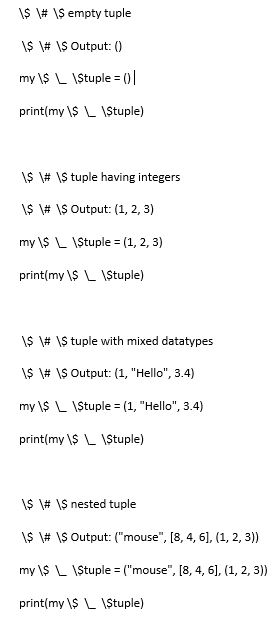
\includegraphics[width=0.1\textwidth]{figures/3afs1.JPG}}
			\caption{}
			\label{3afs1}
			\end{figure}
   
\begin{figure}[ht]
			\centerline{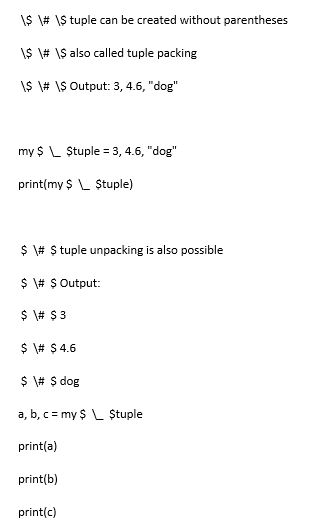
\includegraphics[width=0.1\textwidth]{figures/3afs2.JPG}}
			\caption{}
			\label{3afs2}
			\end{figure}
   

\section{Membuat tuple dengan satu elemen} 
Memiliki satu elemen dalam kurung saja tidak cukup. Kita membutuhkan koma trailing untuk menunjukkan bahwa sebenarnya ada tupel. 
\begin{verbatim}
 $  \#  $ only parentheses is not enough 
 $  \#  $ Output: <class 'str'> 
my $  \_  $tuple = ("hello") 
print(type(my $  \_  $tuple)) 

 $  \#  $ need a comma at the end 
 $  \#  $ Output: <class 'tuple'> 
my $  \_  $tuple~= ("hello",)   
print(type(my $  \_  $tuple)) 

 $  \#  $ parentheses is optional 
 $  \#  $ Output: <class 'tuple'> 
my $  \_  $tuple = "hello", 
print(type(my $  \_  $tuple)) 
\end{verbatim}
\section{Mengakses Elemen dalam Tuple} 
Ada berbagai cara untuk mengakses elemen tuple. 
\subsection{Pengindeksan}
Kita bisa menggunakan operator indeks [] untuk mengakses item di tupel dimana indeks dimulai dari 0. Jadi, tupel yang memiliki 6 elemen akan memiliki indeks dari 0 sampai 5. Mencoba mengakses elemen lain yang (6, 7, ...) akan menghasilkan IndexError. Indeks harus berupa bilangan bulat, jadi kita tidak bisa menggunakan float atau jenis lainnya. Ini akan menghasilkan TypeError. Demikian juga, tuple bersarang diakses menggunakan pengindeksan nested, seperti yang ditunjukkan pada contoh di bawah ini. 
\begin{verbatim}
my $  \_  $tuple = ('p','e','r','m','i','t') 

 $  \#  $ Output: 'p' 
print(my $  \_  $tuple[0]) \

 $  \#  $ Output: 't' 
print(my $  \_  $tuple[5]) 

 $  \#  $ index must be in range 
 $  \#  $ If you uncomment line 14, 
 $  \#  $ you will get an error. 
 $  \#  $ IndexError: list index out of range 

 $  \#  $print(my $  \_  $tuple[6]) 

 $  \#  $ index must be an integer 
 $  \#  $ If you uncomment line 21, 
 $  \#  $ you will get an error. 
 $  \#  $ TypeError: list indices must be integers, not float 

 $  \#  $my $  \_  $tuple[2.0] 

 $  \#  $ nested tuple 
n $  \_  $tuple = ("mouse", [8, 4, 6], (1, 2, 3)) 

 $  \#  $ nested index 
 $  \#  $ Output: 's' 
print(n $  \_  $tuple[0][3]) 

 $  \#  $ nested index 
 $  \#  $ Output: 4 
print(n $  \_  $tuple[1][1]) 
\end{verbatim}
\subsection{Slicing} 
Kita bisa mengakses berbagai item dalam tupel dengan menggunakan operator pengiris - titik dua ":". 
\begin{verbatim}
my $  \_  $tuple = ('p','r','o','g','r','a','m','i','z') 

 $  \#  $ elements 2nd to 4th 
 $  \#  $ Output: ('r', 'o', 'g') 
print(my $  \_  $tuple[1:4]) 

 $  \#  $ elements beginning to 2nd 
 $  \#  $ Output: ('p', 'r') 
print(my $  \_  $tuple[:-7]) 

 $  \#  $ elements 8th to end 
 $  \#  $ Output: ('i', 'z') 
print(my $  \_  $tuple[7:]) 

 $  \#  $ elements beginning to end 
 $  \#  $ Output: ('p', 'r', 'o', 'g', 'r', 'a', 'm', 'i', 'z') 
print(my $  \_  $tuple[:]) 
\end{verbatim}
\section{Mengubah Tuple} 
Tidak seperti daftar, tupel tidak dapat diubah. Ini berarti elemen tupel tidak dapat diubah begitu telah ditetapkan. Tapi, jika elemen itu sendiri adalah datatype yang bisa berubah seperti daftar, item nested-nya bisa diubah. Kita juga bisa menugaskan tuple ke nilai yang berbeda \(reassignment\). 
\begin{verbatim}
my $  \_  $tuple = (4, 2, 3, [6, 5]) 

 $  \#  $ we cannot change an element 
 $  \#  $ If you uncomment line 8 
 $  \#  $ you will get an error: 
 $  \#  $ TypeError: 'tuple' object does not support item assignment 

 $  \#  $my $  \_  $tuple[1] = 9 

 $  \#  $ but item of mutable element can be changed 
 $  \#  $ Output: (4, 2, 3, [9, 5]) 
my $  \_  $tuple[3][0] = 9 
print(my $  \_  $tuple) 

 $  \#  $ tuples can be reassigned 
 $  \#  $ Output: ('p', 'r', 'o', 'g', 'r', 'a', 'm', 'i', 'z') 
my $  \_  $tuple = ('p','r','o','g','r','a','m','i','z') 
print(my $  \_  $tuple) 
\end{verbatim}
\section{Python Tuples} 
Tutorial Tuple Python menjelaskan tupel dan bagaimana menggunakannya dengan Python. Dengan Python, tupel hampir sama dengan daftar. Jadi, mengapa kita harus menggunakannya? Satu perbedaan utama antara tupel dan daftar adalah bahwa tupel tidak dapat diubah. Artinya, Anda tidak dapat menambahkan, mengubah, atau menghapus elemen dari tuple. Tupel mungkin tampak aneh pada awalnya, tapi ada alasan bagus mengapa mereka tidak bisa berubah. Sebagai pemrogram, kita mengacaukan sesekali. Kami mengubah variabel yang tidak ingin kami ubah, dan terkadang, kami hanya ingin hal-hal menjadi konstan sehingga kami tidak sengaja mengubahnya nanti. Namun, jika kita mengubah pikiran kita, kita juga bisa mengubah tupel menjadi daftar atau daftar menjadi tupel. Faktanya adalah kita perlu membuat usaha sadar untuk mengatakan Python, saya ingin mengubah tupel ini menjadi sebuah daftar sehingga saya bisa memodifikasinya. Cukup mengoceh, mari kita lihat sebuah tuple beraksi!
Otak Anda masih sakit dari pelajaran terakhir? Jangan khawatir, yang satu ini akan membutuhkan sedikit pemikiran. Kita akan kembali ke sesuatu yang sederhana - variabel - tapi sedikit lebih mendalam. Pikirkanlah - variabel menyimpan satu bit informasi. Mereka mungkin muntah-muntah (tidak di karpet ...) informasi itu kapan saja, dan sedikit informasi mereka dapat berubah sewaktu-waktu. Variabel sangat bagus dengan apa yang mereka lakukan - menyimpan informasi yang mungkin berubah seiring berjalannya waktu. 

Tapi bagaimana jika Anda perlu menyimpan daftar panjang informasi, yang tidak berubah dari waktu ke waktu? Katakanlah, misalnya, nama bulan dalam setahun. Atau mungkin daftar panjang informasi, itu memang berubah seiring berjalannya waktu? Katakanlah, misalnya, nama semua kucing Anda. Anda mungkin mendapatkan kucing baru, beberapa mungkin mati, beberapa mungkin menjadi makan malam Anda (kami harus menukar resep!). Bagaimana dengan buku telepon? Untuk itu Anda perlu melakukan sedikit referensi - Anda akan memiliki daftar nama, dan dilampirkan pada masing-masing nama tersebut, nomor teleponnya. Bagaimana Anda melakukannya?

Untuk ketiga masalah ini, Python menggunakan tiga solusi berbeda - daftar, tupel, dan kamus: 
\begin{enumerate}
\item Daftar adalah apa yang mereka tampaknya - daftar nilai. Masing-masing diberi nomor, mulai dari nol - yang pertama diberi nomor nol, yang kedua 1, yang ketiga 2, dll. Anda dapat menghapus nilai dari daftar, dan menambahkan nilai baru sampai akhir. Contoh: nama kucing Anda banyak. 
\item Tupel sama seperti daftar, tapi Anda tidak dapat mengubah nilainya. Nilai yang Anda berikan terlebih dahulu, adalah nilai yang Anda pakai untuk sisa program. Sekali lagi, setiap nilai diberi nomor mulai dari nol, untuk referensi mudah. Contoh: nama bulan dalam setahun. 
\item Kamus serupa dengan apa yang namanya namanya - kamus. Dalam kamus, Anda memiliki 'indeks' kata-kata, dan untuk masing-masing definisi. Dengan kata Python, kata itu disebut 'kunci', dan definisi sebuah 'nilai'. Nilai dalam kamus tidak diberi nomor - keduanya tidak sesuai urutan tertentu, kuncinya adalah hal yang sama. (Setiap tombol harus unik, meskipun!) Anda dapat menambahkan, menghapus, dan memodifikasi nilai-nilai di kamus. Contoh: buku telepon jadi ada yang lebih hidup dari pada nama kucing Anda. Anda perlu menghubungi saudara perempuan, ibu, anak laki-laki, pria buah, dan orang lain yang perlu tahu bahwa kucing favorit mereka sudah meninggal. Untuk itu Anda membutuhkan buku telepon. 
\end{enumerate}
Sekarang, daftar yang telah kami gunakan di atas tidak sesuai untuk buku telepon. Anda perlu mengetahui nomor berdasarkan nama seseorang - bukan sebaliknya, seperti yang kami lakukan pada kucing. Dalam contoh bulan dan kucing, kami memberi nomor komputer, dan itu memberi kami sebuah nama. Kali ini kami ingin memberi nama komputer, dan ini memberi kami nomor. Untuk ini kita butuh kamus.

Jadi bagaimana kita membuat kamus? Letakkan peralatan pengikat Anda, bukan itu yang maju. ingat, kamus memiliki kunci, dan nilai. Dalam buku telepon, Anda punya nama orang, lalu nomor mereka. Melihat kesamaan? Saat pertama kali membuat kamus, sangat mirip membuat tupel atau daftar. Tupel memiliki (dan) benda, daftar memiliki [dan] benda. Tebak apa! kamus memiliki \$  \{  \$dan \$  \}  \$ hal - kurung kurawal. Berikut adalah contoh di bawah ini, menampilkan kamus dengan empat nomor telepon di dalamnya: 

Selain List, Tuple juga merupakan tipe data urutan \(sequence data type\) yang secara fungsi sama dengan List. Namun Tuple berbeda sifatnya, yaitu Tuple bersifat immutable yang mana data di dalam Tuple tidak dapat kita ubah atau dihapuskan. Sebuah Tuple terdiri dari beberapa nilai yang dipisahkan oleh tanda koma (‘,’). Tidak seperti List, tipe data Tuple ditandai dengan tanda kurung \"()\".

Tupel berguna untuk mewakili bahasa lain yang sering disebut catatan \- beberapa informasi terkait yang dimiliki bersama, seperti catatan siswa Anda. Tidak ada deskripsi tentang apa yang masing-masing bidang ini berarti, tapi kita bisa menebaknya. Sebuah tupel memungkinkan kita \"mengumpulkan\" informasi yang terkait dan menggunakannya sebagai satu hal.


chapter{Date and Time}
input{DateTimeFix}

\chapter{Dictionary}
\section{Python Dictionary}
Dictionary Python adalah kumpulan pasangan kunci:nilai (selanjutnya disebut: key-value) yang tak berurutan. Dictionary Python ini sama halnya dengan hash-table atau array-asosiatif di pemrograman Perl.

Suatu kunci (key) pada Dictionary bersifat Unique (unik), yang artinya adalah satu kunci hanya memiliki satu nilai. Aturan penulisannya berupa key:value. Sebuah Dictionary ditandai dengan adanya kurung kurawal “{}”. Setiap pasangan key:value dipisah dengan tanda koma. 

Setiap kunci dipisahkan dari nilainya oleh titik dua (:), item dipisahkan oleh koma, dan semuanya tertutup dalam kurung kurawal. Kamus kosong tanpa barang ditulis hanya dengan dua kurung kurawal, seperti ini:  \$  \{  \$ \$  \}  \$.

Kunci unik dalam kamus sementara nilai mungkin tidak. Nilai kamus bisa berupa tipe apa pun, namun kunci harus berupa tipe data yang tidak berubah seperti string, angka, atau tupel.

Dictionary menyediakan wadah yang sangat berguna yang memungkinkan kita mencari nilai menggunakan kunci\cite{oliphant2007python}. Dalam sebuah Dictionary tidak boleh ada dua key yang sama, maka memberikan nilai ke key yang sudah ada akan menghapus nilai yang lama. Untuk menambah key baru, Python memiliki syntax yang sama. Ini bisa menimbulkan kerancuan pada saat akan melakukan penambahan key baru, tapi ternyata hanya mengubah key yang sudah ada. Sebagai catatan, key yang baru terletak di bagian tengah bukan di belakang. Hal tersebut kebetulan saja, karena sebenarnya pada Dictionary memang tidak ada standar pengurutan yang berlaku.

\subsection{Accessing Values in Dictionary}
Untuk mengakses elemen kamus, Anda dapat menggunakan tanda kurung siku yang sudah dikenal bersama dengan kunci untuk mendapatkan nilainya. Berikut adalah contoh sederhana :
\begin{verbatim}  
  \$  \#  \$!/usr/bin/python
  dict =  \$  \{  \$'Name': 'Zara', 'Age': 7, 'Class': 'First' \$  \}  \$ 
 print "dict['Name']: ", dict['Name'] 
 print "dict['Age']: ", dict['Age']
\end{verbatim}
Bila kode diatas dieksekusi, maka menghasilkan hasil sebagai berikut :
dict['Name']:~ Zara
dict['Age']:~ 7 
Jika kita mencoba mengakses item data dengan sebuah kunci, yang bukan bagian dari kamus, kita mendapatkan error sebagai berikut :
\begin{verbatim} 
\$  \#  \$!/usr/bin/python
dict =  \$  \{  \$'Name': 'Zara', 'Age': 7, 'Class': 'First' \$  \}  \$ 
print "dict['Alice']: ", dict['Alice']
\end{verbatim}
Bila kode diatas dieksekusi, maka menghasilkan hasil sebagai berikut :
\begin{verbatim}
dict['Alice']: 
Traceback (most recent call last):
~~ File "test.py", line 4, in <module>
~~~~~  \print "dict['Alice']: ", dict['Alice']; 
KeyError: 'Alice' 
\end{verbatim}

\subsection{Updating Dictionary}
Anda dapat memperbarui kamus dengan menambahkan entri baru atau pasangan nilai kunci, memodifikasi entri yang ada, atau menghapus entri yang ada seperti yang ditunjukkan di bawah ini dalam contoh sederhana :
\begin{verbatim}
\$  \#  \$!/usr/bin/python 
  dict =  \$  \{  \$'Name': 'Zara', 'Age': 7, 'Class': 'First' \$  \}  \$ 
  dict['Age'] = 8;  \$  \#  \$ update existing entry
  dict['School'] = "DPS School";  \$  \#  \$ Add new entry
  print "dict['Age']: ", dict['Age']
  print "dict['School']: ", dict['School']
\end{verbatim}
Bila kode diatas dieksekusi, maka menghasilkan hasil sebagai berikut : 
  dict['Age']:~ 8 
  dict['School']:~ DPS School 
  
\subsection{Delete Dictionary Elements}
Anda dapat menghapus elemen kamus individual atau menghapus keseluruhan isi kamus. Anda juga dapat menghapus seluruh kamus dalam satu operasi. 
Untuk menghapus seluruh kamus secara eksplisit, cukup gunakan del statement. Berikut adalah contoh sederhana : 
\begin{verbatim}   
   \$  \#  \$!/usr/bin/python
  dict =  \$  \{  \$'Name': 'Zara', 'Age': 7, 'Class': 'First' \$  \}  \$
  del dict['Name'];  \$  \#  \$ remove entry with key 'Name'
  dict.clear();~~~~  \$  \#  \$ remove all entries in dict 
  del dict~;~~~~~~   \$  \#  \$ delete entire dictionary 
  print "dict['Age']: ", dict['Age'] 
  print "dict['School']: ", dict['School']
\end{verbatim}  
Ini menghasilkan hasil berikut. Perhatikan bahwa pengecualian diajukan karena setelah kamus del dict tidak ada lagi - 
  dict['Age']: 
  Traceback (most recent call last): 
~   File "test.py", line 8, in <module> 
~~~     print "dict['Age']: ", dict['Age']; 
  TypeError: 'type' object is unsubscriptable 
Note: del () metode dibahas di bagian selanjutnya. 

\subsection{Properties of Dictionary Keys} 
Nilai kamus tidak memiliki batasan. Mereka bisa menjadi objek Python yang sewenang-wenang, baik objek standar atau objek yang ditentukan pengguna. Namun, hal yang sama tidak berlaku untuk kunci. 
Ada dua hal penting yang perlu diingat tentang kunci kamus – 
Lebih dari satu entri per kunci tidak diperbolehkan. Yang berarti tidak ada kunci duplikat yang diperbolehkan. Ketika kunci duplikat ditemui selama penugasan, tugas terakhir akan menang. Sebagai contoh – 
\begin{verbatim}   
   \$  \#  \$!/usr/bin/python 
  dict =  \$  \{  \$'Name': 'Zara', 'Age': 7, 'Name': 'Manni' \$  \}  \$ 
  print "dict['Name']: ", dict['Name']
\end{verbatim}  
Bila kode diatas dieksekusi, maka menghasilkan hasil sebagai berikut : 
  dict['Name']:~ Manni 
(b) Tombol harus tidak berubah. Yang berarti Anda bisa menggunakan string, angka atau tupel sebagai tombol kamus tapi sesuatu seperti ['key'] tidak diperbolehkan. Berikut adalah contoh sederhana: 
\begin{verbatim}   
   \$  \#  \$!/usr/bin/python 
  dict =  \$  \{  \$['Name']: 'Zara', 'Age': 7 \$  \}  \$ 
  print "dict['Name']: ", dict['Name']
\end{verbatim}
Bila kode diatas dieksekusi, maka menghasilkan hasil sebagai berikut : 
  Traceback (most recent call last): 
~~     File "test.py", line 3, in <module> 
~~~~~     dict =  \$  \{  \$['Name']: 'Zara', 'Age': 7 \$  \}  \$; 
  TypeError: list objects are unhashable 
Built-in Dictionary Functions  \$  \&  \$ Methods  \$ - \$ 
Python includes the following dictionary functions  \$ - \$ 
Python includes following dictionary methods  \$ - \$ 

\subsection{Dictionaries Introductions} 
Kami sudah mengenal daftar di bab sebelumnya. Di bab kusus Python online kami akan mempresentasikan kamus dan operator dan metode pada kamus. Program atau skrip Python tanpa daftar dan kamus hampir tidak dapat dibayangkan. Seperti daftar kamus yang bisa dengan mudah diubah, bisa menyusut dan berkembang ad libitum pada saat run time. Mereka menyusut dan tumbuh tanpa perlu membuat salinan. Kamus dapat dimuat dalam daftar dan sebaliknya. Tapi apa perbedaan antara daftar dan kamus? Daftar diurutkan dari objek, sedangkan kamus tidak berurutan. Tapi perbedaan utamanya adalah item dalam kamus diakses melalui kunci dan tidak melalui posisinya. Kamus adalah array asosiatif (juga dikenal sebagai hash). Kunci kamus mana pun dikaitkan (atau dipetakan) ke sebuah nilai. Nilai kamus bisa berupa tipe data Python. Jadi kamus adalah pasangan kunci-nilai tak berurutan. 
Kamus tidak mendukung urutan operasi dari jenis data urutan seperti string, tupel dan daftar. Kamus termasuk tipe pemetaan built-in. Mereka adalah satu-satunya wakil semacam ini! 
Di akhir bab ini, kami akan menunjukkan bagaimana kamus dapat diubah menjadi satu daftar, berisi (kunci, nilai) -tupel atau dua daftar, yaitu satu dengan kunci dan satu dengan nilainya. Transformasi ini bisa dilakukan secara terbalik juga. 

\subsection{How to create a dictionary?}
Membuat kamus sama mudahnya dengan menempatkan item dalam kurung kurawal  \$  \{  \$ \$  \}  \$ dipisahkan dengan koma. Item memiliki kunci dan nilai yang sesuai dinyatakan sebagai pasangan, kunci: nilai. Sementara nilai dapat berupa tipe data apa pun dan dapat diulang, kunci harus terdiri dari tipe yang tidak dapat diubah (string, number atau tupel dengan elemen yang tidak berubah) dan harus unik. 
\begin{verbatim}
   \$  \#  \$ empty dictionary 
  my \$  \_  \$dict =  \$  \{  \$ \$  \}  \$ 
   \$  \#  \$ dictionary with integer keys 
  my \$  \_  \$dict =  \$  \{  \$1: 'apple', 2: 'ball' \$  \}  \$ 
   \$  \#  \$ dictionary with mixed keys 
  my \$  \_  \$dict =  \$  \{  \$'name': 'John', 1: [2, 4, 3] \$  \}  \$ 
   \$  \#  \$ using dict() 
  my \$  \_  \$dict = dict( \$  \{  \$1:'apple', 2:'ball' \$  \}  \$) 
   \$  \#  \$ from sequence having each item as a pair 
  my \$  \_  \$dict = dict([(1,'apple'), (2,'ball')])
\end{verbatim}
Seperti yang bisa Anda lihat di atas, kita juga bisa membuat kamus menggunakan fungsi built-in dict (). 

\subsection{How to access elements from a dictionary?} 
Sementara pengindeksan digunakan dengan jenis wadah lain untuk mengakses nilai, kamus menggunakan tombol. Kunci dapat digunakan baik di dalam tanda kurung siku atau dengan metode get (). Perbedaan saat menggunakan get () adalah mengembalikan Elemen alih-alih KeyError, jika kuncinya tidak ditemukan. 
\begin{verbatim}
  my \$  \_  \$dict =  \$  \{  \$'name':'Jack', 'age': 26 \$  \}  \$ 
   \$  \#  \$ Output: Jack 
  print(my \$  \_  \$dict['name']) 
   \$  \#  \$ Output: 26 
  print(my \$  \_  \$dict.get('age')) 
   \$  \#  \$ Trying to access keys which doesn't exist throws error 
   \$  \#  \$ my \$  \_  \$dict.get('address') 
   \$  \#  \$ my \$  \_  \$dict['address'] 
\end{verbatim}   
Saat menjalankan program, hasilnya adalah: 
Jack 
26 

\subsection{How to change or add elements in a dictionary?}
Kamus bisa berubah-ubah. Kita bisa menambahkan item baru atau mengubah nilai barang yang ada menggunakan operator penugasan. 
Jika kuncinya sudah ada, nilai akan diperbarui, jika ada kunci baru: pasangan nilai ditambahkan ke kamus. 
Script.py
\begin{verbatim}
  my \$  \_  \$dict =  \$  \{  \$'name':'Jack', 'age': 26 \$  \}  \$ 
   \$  \#  \$ update value 
  my \$  \_  \$dict['age'] = 27 
   \$  \#  \$Output:  \$  \{  \$'age': 27, 'name': 'Jack' \$  \}  \$ 
  print(my \$  \_  \$dict) 
   \$  \#  \$ add item 
  my \$  \_  \$dict['address']~= 'Downtown'   
   \$  \#  \$ Output:  \$  \{  \$'address': 'Downtown', 'age': 27, 'name': 'Jack' \$  \}  \$ 
  print(my \$  \_  \$dict). 
\end{verbatim}  
Saat menjalankan program, hasilnya adalah: 

 \$  \{  \$'name': 'Jack', 'age': 27 \$  \}  \$ 
 \$  \{  \$'name': 'Jack', 'age': 27, 'address': 'Downtown' \$  \}  \$ 
 
\subsection{How to delete or remove elements from a dictionary?}
Kita bisa menghapus item tertentu dalam kamus dengan menggunakan metode pop (). Metode ini menghilangkan item dengan tombol yang disediakan dan mengembalikan nilainya. 
Metodenya, popitem () dapat digunakan untuk menghapus dan mengembalikan item yang sewenang-wenang (key, value) membentuk kamus. Semua item dapat dihapus sekaligus dengan menggunakan metode clear (). 
Kita juga bisa menggunakan kata kunci del untuk menghapus setiap item atau keseluruhan kamus itu sendiri. 
Scrip.py
\begin{verbatim}
   \$  \#  \$ create a dictionary 
  squares~=  \$  \{  \$1:1, 2:4, 3:9, 4:16, 5:25 \$  \}  \$   
   \$  \#  \$ remove a particular item 
   \$  \#  \$ Output: 16 
  print(squares.pop(4))~  
   \$  \#  \$ Output:  \$  \{  \$1: 1, 2: 4, 3: 9, 5: 25 \$  \}  \$ 
  print(squares) 
   \$  \#  \$ remove an arbitrary item 
   \$  \#  \$ Output: (1, 1) 
  print(squares.popitem()) 
   \$  \#  \$ Output:  \$  \{  \$2: 4, 3: 9, 5: 25 \$  \}  \$ 
  print(squares) 
   \$  \#  \$ delete a particular item 
  del~squares[5]   
   \$  \#  \$ Output:  \$  \{  \$2: 4, 3: 9 \$  \}  \$ 
  print(squares) 
   \$  \#  \$ remove all items 
  squares.clear() 
   \$  \#  \$ Output:  \$  \{  \$ \$  \}  \$ 
  print(squares) 
   \$  \#  \$ delete the dictionary itself 
  del squares 
  \$  \#  \$ Throws Error 
  \$  \#  \$ print(squares)
\end{verbatim}  
When you run the program, the output will be: 
16 
 \$  \{  \$1: 1, 2: 4, 3: 9, 5: 25 \$  \}  \$ 
(1, 1) 
 \$  \{  \$2: 4, 3: 9, 5: 25 \$  \}  \$ 
 \$  \{  \$2: 4, 3: 9 \$  \}  \$ 
 \$  \{  \$ \$  \}  \$ 
Tipe data daftar memiliki beberapa metode lagi. Berikut adalah semua metode daftar objek: 
list.append (x) 
Tambahkan item ke bagian akhir daftar; setara dengan [len (a):] = [x]. 
list.extend (L) 
Perluas daftar dengan menambahkan semua item dalam daftar yang diberikan; setara dengan [len (a):] = L. 
list.insert (i, x) 
Masukkan item pada posisi tertentu. Argumen pertama adalah indeks dari elemen yang sebelum dimasukkan, jadi a.insert (0, x) memasukkan di bagian depan daftar, dan a.insert (len (a), x) setara dengan a.append ( x). 
list.remove (x) 
Hapus item pertama dari daftar yang nilainya x. Ini adalah kesalahan jika tidak ada item seperti itu. 
list.pop ([i]) 
Hapus item pada posisi yang diberikan dalam daftar, dan kembalikan. Jika tidak ada indeks yang ditentukan, a.pop () menghapus dan mengembalikan item terakhir dalam daftar. (Tanda kurung siku di sekitar i pada tanda tangan metode menunjukkan bahwa parameternya adalah opsional, bukankah Anda harus mengetikkan tanda kurung siku pada posisi itu. Anda akan sering melihat notasi ini di Referensi Perpustakaan Python.) 
list.index (x) 
Kembalikan indeks di daftar item pertama yang nilainya x. Ini adalah kesalahan jika tidak ada item seperti itu. 
list.count (x) 
Kembalikan berapa kali x muncul dalam daftar. 
list.sort (cmp = None, key = None, reverse = False) 
Urutkan item daftar di tempat (argumen dapat digunakan untuk kustomisasi sortir, lihat diurutkan () untuk penjelasan mereka). 
list.reverse () 
Membalik unsur daftar, di tempat. 
Nilai Dictionary tidak memiliki batasan. Mereka bisa menjadi objek Python yang sewenang-wenang, baik objek standar atau objek yang ditentukan pengguna. Namun, hal yang sama tidak berlaku untuk key. 
Ada dua hal penting yang harus diingat tentang Dictionary Key. 
Pertama lebih dari satu entri per key tidak diperbolehkan. Yang berarti tidak ada key duplikat yang diperbolehkan. Saat key duplikat ditemui selama penugasan, tugas terakhir akan menang. 
Kedua key harus tidak berubah. Yang berarti Anda bisa menggunakan string, angka atau tuples sebagai tombol kamus tapi sesuatu seperti ['key'] tidak diperbolehkan. 


\chapter{Functions}
\section{Python Functions}
Fungsi adalah blok kode terorganisir dan dapat digunakan kembali yang digunakan untuk melakukan tindakan tunggal dan terkait. Fungsi menyediakan modularitas yang lebih baik untuk aplikasi Anda dan tingkat penggunaan kode yang tinggi. Seperti yang sudah Anda ketahui, Python memberi Anda banyak fungsi built-in seperti cetak (), dll. Tetapi Anda juga dapat membuat fungsi Anda sendiri. Fungsi ini disebut fungsi yang ditentukan pengguna. 

Ada tiga jenis fungsi dengan Python: 
\begin{enumerate}
\item Built-in Functions, seperRekursif ti help () untuk meminta bantuan, min () untuk mendapatkan nilai minimum, print () untuk mencetak objek ke terminal.
\item User-Defined Functions (UDFs), yang merupakan fungsi yang dibuat untuk membantu pengguna
\item Anonymous Functions, yang juga disebut fungsi lambda karena tidak dinyatakan dengan kata kunci def standar.
\end{enumerate}

Keuntungan-keuntungan menggunakan Function, yaitu: 
\begin{enumerate}
\item Program besar dapat di bagi menjadi program-program kecil menggunakan function.
\item Kemudahan mencari error atau kesalahan karena alur logika jelas dan kesalahan dapat ditempatkan pada suatu modul tertentu.
\item Memodifikasi dan memperbaiki program dapat digunakan pada suatu modul tertentu saja tanpa mempengaruhi keseluruhan program.
\item Dapat digunakan lagi (Reusability) oleh program atau fungsi lain.
\item Meminimalkan penulisan perintah yang sama. 
\end{enumerate}

function di Python biasanya mempunyai sebuah parameter dan return statement. Function di Python mempunyai pola sebagai berikut:
\begin{verbatim}
def nama function yang ingin anda buat (param1, param2, ... paramn):
   
   # kode Anda diisi
    return sesuatu
\end{verbatim}    
Tipe data yang dikembalikan bisa bermacam jenis tipe data yang didukung Python. Meskipun parameter yang akan diterima oleh function tersebut. 

\section{Kategori Fungsi}
\begin{enumerate}
\item Standard Library Function ialah fungsi-fungsi yang telah disediakan oleh Interpreter Python dalam file-file atau librarynya.  Misalnya: raw\_input(), input(), print(), open(), len(), max(), min(), abs()  dan lain-lain. 
\item Programme-Defined Function ialah function yang dibuat oleh programmer itu sendiri. Function ini memiliki nama tertentu yang unik dalam programnya, letaknya terpisah dari program utama, dan bisa dijadikan satu ke dalam suatu library yang di buat oleh programmer itu sendiri.
\end{enumerate}

Dalam python terdapat dua buah perintah yang dapat digunakan untuk membuat sebuah fungsi, yaitu def dan lambda. def adalah perintah standar di dalam python untuk mendefinisikan sebuah fungsi. Tidak seperti function dalam bahasa pemrograman compiler seperti C/C++, def dalam bahasa python merupakan perintah yang executable, artinya function yang tidak akan aktif sampai python merunning perintah def tersebut. Sedangkan lambda, dalam python lebih dikenal dengan nama Anonymous Function (Fungsi yang tidak disebutkan namanya). Lambda bukanlah sebuah perintah (statemen) namun lebih kepada ekspresi (expression).


\subsection{Defining a Function} 
Anda dapat menentukan fungsi untuk menyediakan fungsionalitas yang dibutuhkan. Berikut adalah aturan sederhana untuk mendefinisikan fungsi dengan Python. 
\begin{enumerate}
\item Blok fungsi dimulai dengan defensi kata kunci diikuti oleh nama fungsi dan tanda kurung (()).
\item Setiap parameter masukan atau argumen harus ditempatkan di dalam tanda kurung ini. Anda juga dapat menentukan parameter di dalam tanda kurung ini.
\item Pernyataan fungsi pertama dapat berupa pernyataan opsional - string dokumentasi fungsi atau docstring.
\item Blok kode dalam setiap fungsi dimulai dengan titik dua (:) dan indentasi.
\item Pernyataan kembali [ekspresi] keluar dari sebuah fungsi, secara opsional menyampaikan kembali ekspresi ke pemanggil. Pernyataan pengembalian tanpa argumen sama dengan return None.
\end{enumerate}

\subsection{Parameter Fungsi} 
Parameter Fungsi adalah sebuah fungsi yang dapat mempunyai daftar argumen (parameter) atau tidak. 

\subsubsection{Parameter Posisi} 
Parameter Posisi merupakan parameter fungsi pada urutan posisi yang valid. Saat pemanggilan fungsi, parameter itu diharuskan sesuai dengan jumlah parameter yang sudah didefinisikan. 

Contoh : 
\begin{verbatim}
def perhitunan (k,l) :
            m=k+l
            return m
perhitungan (4,5)
0utput = 9
\end{verbatim}

\subsubsection{Parameter Nama} 
Parameter Nama adalah Dipanggilnya fungsi  nilai pada parameternya dijelaskan langsung dari nama parameternya. 

Contoh :
\begin{verbatim}
def totalTransfer(hari, uangTransfer):
            gaji= hari*uangTransfer
            return gaji
totalTransfer(hari=20,uangTransfer=20000)
Output = 400000
\end{verbatim}

\subsubsection{Parameter Default}
Parameter default adalah nilai yang diambil ke parameter pada saat pendefinisian fungsi.
Contoh :
\begin{verbatim}
def koin (ratusan, ribuan=5) :
Print “koin ratusannya adalah ; “, ratusan;
Print “koin ribuannya adalah ; “, ribuan;
Uang(7)
Output : 7 dan 5 , nilai default yang digunakan.
\end{verbatim}

\subsubsection{Parameter Bertipe List} 
Parameter Bertipe List adalah satu parameter yang diawali oleh tanda  *. 
Contoh :
\begin{verbatim}
def angka(*bilangan) ;
            Print angka
angka (2,7,9)
Output : (2,7,9)
\end{verbatim}

\section{Syntax} 
Berikut adalah contoh program kalkulator menggunakan Function pada Python : 
\begin{verbatim}
def menu()
    print "Hallo Guys :) Selamat Datang di Program Kalkulator"
    print "Pilih Operasi Bilangan :"
    print " "
    print "1) Penjumlahan"
    print "2) Pengurangan"
    print "3) Perkalian"
    print "4) Pembagian"
    print "5) Keluar Program"
    print " "
    return input ("Pilih Operasi Matematikanya : ")

# Function untuk Penjumlahan
def tbh(a,b):
    print a, "+", b, "=", a + b

# Function untuk Pengurangan
def kur(a,b):
    print b, "+", a, "=", b + a

# Function untuk Perkalian
def kal(a,b):
    print a, "*", b, "=", a * b

# Function untuk Pembagian
def bag(a,b):
    print a, "/", b, "=", a / b

loop = 1
choice = 0
while loop == 1:
    choice = menu()
    if choice == 1:
        tbh(input("Tambahkan Ini: "),input("Dengan ini: "))
    elif choice == 2:
        kur(input("Kurangkan Ini: "),input("Dengan ini: "))
    elif choice == 3:
        kur(input("Kalikan Ini: "),input("Dengan ini: "))
    elif choice == 4:
        kur(input("Bagikan Ini: "),input("Dengan ini: "))
    elif choice == 5:
        loop = 0

print "GoodBye :( Terimakasih Telah Menggunakan calc.py :)"
\end{verbatim}

Berikut contoh Program Mencetak Menu dan Menghitung Luas menggunakan Function pada Python : 
\begin{verbatim}
def menu(): 
print "Menu Options" 
print 
print "1. Segitiga" 
print "2. Persegi Panjang" 
print "3. Lingkaran" 
print "4. Keluar" 

def segitiga(): 
print "Menghitung Luas Segitiga" 
a = input("Tambahkan Alas : ") 
t = input("Tambahkan Tinggi : ") 
luas = (a*t)/2 
print "Luas Segitiga yaitu ",luas 
print 
print "Coba lagi [Y/N]? " 
back = raw_input().upper() 
if back == "Y": 
menu() 
else: 
exit()

def persegipanjang(): 
print "Menghitung Luas Persegi Panjang" 
p = input("Masukkan Panjang : ") 
l = input("Masukkan Lebar : ") 
luas = p*l 
print "Luas Persegi Panjang yaitu ",luas 
print 
print "Coba lagi [Y/N]? " 
back = raw_input().upper() 
if back == "Y": 
menu() 
else: 
exit() 

def lingkaran(): 
print "Menghitung Luas Lingkaran" 
r = input("Tambahkan Jari-Jari : ") 
luas = 3.14*(r**2) 
print "Luas Lingkaran yaitu ",luas 
print 
print "Coba lagi [Y/N]? " 
back = raw_input().upper() 
if back == "Y": 
menu() 
else: 
exit() 

#Program Perhitungan Luas 
print "Selamat Bahagia di Program Menghitung Luas" 
print "-----------------------------------------------" 
print 
menu() 
while l: 
#input 
pilih = input("Masukkan options : ") 
if pilih == 1: 
Segitiga() 
elif pilih == 2: 
Persegi Panjang() 
elif pilih == 3: 
Lingkaran() 
elif pilih == 4: 
print "\n"*100 
break 
else: 
print "Sorry Option yang di masukkan tidak ada" 
print "Coba lagi [Y/N] ? " 
coba = raw_input().upper() 
if coba == "Y": 
menu() 
else: 
print "\n"*100 
break
\end{verbatim}

\begin{verbatim}
def functionname( parameters ): 
"function \$  \_  \$docstring"
function \$  \_  \$suite 
return [expression] 
\end{verbatim}
Secara default, parameter memiliki perilaku posisi dan Anda perlu memberi tahu mereka dengan urutan yang sama seperti yang ditetapkan. 
Example:
Fungsi berikut mengambil string sebagai parameter masukan dan mencetaknya di layar standar.
\begin{verbatim}
def printme( str ): 
"This prints a passed string into this function" 
print str 
return \par
\end{verbatim}
\section{Calling a Function} 
Mendefinisikan sebuah fungsi hanya memberinya sebuah nama, menentukan parameter yang akan disertakan dalam fungsi dan menyusun blok kode. Setelah struktur dasar fungsi selesai, Anda dapat menjalankannya dengan memanggilnya dari fungsi lain atau langsung dari prompt Python. Berikut adalah contoh untuk memanggil fungsi printme ().
\begin{verbatim}
\$  \#  \$!/usr/bin/python 

\$  \#  \$ Function definition is here
def printme( str ): 
"This prints a passed string into this function" 
print str
return; 
\$  \#  \$ Now you can call printme function

printme("I'm first call to user defined function!")
printme("Again second call to the same function") 
\end{verbatim}
Bila kode diatas dieksekusi, maka menghasilkan hasil sebagai berikut 

I'm first call to user defined function! 
Again second call to the same function 

\section{Pass by reference vs value}
Semua parameter (argumen) dalam bahasa Python dilewatkan dengan referensi. Ini berarti jika Anda mengubah parameter yang mengacu pada suatu fungsi, perubahan tersebut juga mencerminkan kembali fungsi pemanggilan. Sebagai contoh:
\begin{verbatim}
\$  \#  \$!/usr/bin/python 

\$  \#  \$ Function definition is here 
def changeme( mylist ): 
"This changes a passed list into this function" 
mylist.append([1,2,3,4]); 
"Values inside the function: ", mylist

return


\$  \#  \$ Now you can call changeme function 
mylist = [10,20,30]; 
changeme( mylist );
print "Values outside the function: ", mylist
\end{verbatim}
Di sini, kita mempertahankan referensi objek yang dilewati dan menambahkan nilai pada objek yang sama. Jadi, ini akan menghasilkan hasil sebagai berikut:
\begin{verbatim}
Values~inside the function:  [10, 20, 30, [1, 2, 3, 4]] 
Values~outside the function:  [10, 20, 30, [1, 2, 3, 4]] 
\end{verbatim}
Ada satu contoh lagi di mana argumen dilewatkan melalui referensi dan rujukannya ditimpa di dalam fungsi yang disebut. 
\begin{verbatim}
\$  \# \$!/usr/bin/python 
\$  \#  \$ Function definition is here 
def changeme( mylist ): 
"This changes a passed list into this function" 
~~ mylist = [1,2,3,4];  \$  \#  \$ This would assig new reference in mylist 
~~ print "Values inside the function: ", mylist 

~~ return 

\$  \#  \$ Now you can call changeme function 

mylist = [10,20,30]; 

changeme( mylist ); 

print "Values outside the function: ", mylist 
\end{verbatim}
Parameter mylist adalah local ke fungsi changeme. Mengubah mylist dalam fungsi tidak mempengaruhi mylist. Fungsi ini tidak menghasilkan apa-apa dan akhirnya ini akan menghasilkan hasil sebagai berikut: 
\begin{verbatim}
Values~inside the function:  [1, 2, 3, 4] 

Values~outside the function:  [10, 20, 30] 

Function Arguments
\end{verbatim}
Anda dapat memanggil fungsi dengan menggunakan jenis argumen formal berikut: 
\begin{verbatim}
\$ \bullet \$ Argumen yang dibutuhkan
\$ \bullet \$ Argumen kata kunci 

\$ \bullet \$ Argumen baku

\$ \bullet \$ Argumen panjang variable
\end{verbatim}
\section{Required arguments} 
Argumen yang diperlukan adalah argumen yang diberikan ke sebuah fungsi dalam urutan posisi yang benar. Di sini, jumlah argumen dalam pemanggilan fungsi harus sesuai persis dengan definisi fungsi. Untuk memanggil fungsi printme (), Anda pasti perlu melewati satu argumen, jika tidak maka akan memberikan kesalahan sintaks sebagai berikut :
\begin{verbatim}
\$  \#  \$!/usr/bin/python 
\$  \#  \$ Function definition is here 
def printme( str ): 

~~  "This prints a passed string into this function" 

~~  print str

~~  return;

\$  \#  \$ Now you can call printme function 

printme() 
\end{verbatim}
Bila kode diatas dieksekusi, maka menghasilkan hasil sebagai berikut: 
\begin{verbatim}
Traceback (most recent call last): 

 ~ File "test.py", line 11, in <module> 
~~~ printme();

 TypeError: printme() takes exactly 1 argument (0 given) 
\end{verbatim}
\section{Keyword arguments} 
Argumen kata kunci terkait dengan pemanggilan fungsi. Bila Anda menggunakan argumen kata kunci dalam pemanggilan fungsi, penelepon mengidentifikasi argumen berdasarkan nama parameter. Hal ini memungkinkan Anda melewatkan argumen atau menempatkannya agar tidak bermasalah karena penerjemah Python dapat menggunakan kata kunci yang diberikan agar sesuai dengan nilai parameter. Anda juga dapat membuat panggilan kata kunci ke fungsi printme () dengan cara berikut - 
\begin{verbatim}
\$  \#  \$!/usr/bin/python

\$  \#  \$ Function definition is here

 def printme( str ): 

~~ "This prints a passed string into this function" 

~~ print str 

~~ return; 

 \$  \#  \$ Now you can call printme function 

printme( str = "My string") 
\end{verbatim}
Bila kode diatas dieksekusi, maka menghasilkan hasil sebagai berikut:

My string 

Contoh berikut memberikan gambaran yang lebih jelas. Perhatikan bahwa urutan parameter tidak masalah. 
\begin{verbatim}
\$  \#  \$!/usr/bin/python 

\$  \#  \$ Function definition is here 

def printinfo( name, age ):

~~ "This prints a passed info into this function"

~~ print "Name: ", name 

~~ print "Age ", age 

~~ return; 


\$  \#  \$ Now you can call printinfo function 
printinfo( age=50, name="miki" )
\end{verbatim}
Bila kode diatas dieksekusi, maka menghasilkan hasil sebagai berikut:
Name:\~ miki

Age\~ 50 


\section{Default arguments} 
Argumen default adalah argumen yang mengasumsikan nilai default jika nilai tidak diberikan dalam pemanggilan fungsi untuk argumen itu. Contoh berikut memberi ide pada argumen default, ini mencetak usia default jika tidak lulus.
\begin{verbatim}
\$  \#  \$!/usr/bin/python

\$  \#  \$ Function definition is here 
def printinfo( name, age = 35 ): 
~~ "This prints a passed info into this function"
~~ print "Name: ", name 
~~ print "Age ", age 

~~ return;

\$  \#  \$ Now you can call printinfo function

printinfo( age=50, name="miki" ) 

printinfo( name="miki" ) 
\end{verbatim}
Bila kode diatas dieksekusi, maka menghasilkan hasil sebagai berikut

Name:\~ miki 

Age\~ 50 

Name:\~ miki

Age\~ 35 

\section{Variable-length arguments} 
Anda mungkin perlu memproses sebuah fungsi untuk argumen lebih banyak daripada yang Anda tentukan saat menentukan fungsinya. Argumen ini disebut variable-lengtharguments dan tidak disebutkan dalam definisi fungsi, tidak seperti argumen yang dibutuhkan dan standar. 

Sintaks untuk fungsi dengan argumen variabel non-kata kunci adalah ini :
\begin{verbatim}
def functionname([formal \$  \_  \$args,] *var \$  \_  \$args \$  \_  \$tuple ): 

~~ "function \$  \_  \$docstring" 

~~ function \$  \_  \$suite 

~~ return [expression]
\end{verbatim}
Tanda asterisk (*) ditempatkan sebelum nama variabel yang menyimpan nilai dari semua argumen variabel nonkeyword. Tuple ini tetap kosong jika tidak ada argumen tambahan yang ditentukan selama pemanggilan fungsi. Berikut adalah contoh sederhana : 
\begin{verbatim}
\$  \#  \$!/usr/bin/python 

\$  \#  \$ Function definition is here 

def printinfo( arg1, *vartuple ): 

~~ "This prints a variable passed arguments" 

~~ print "Output is: " 
~~ print arg1
~~ for var in vartuple:
~~~~~ print var 
~~ return; 

\$  \#  \$ Now you can call printinfo function
printinfo( 10 ) 
printinfo( 70, 60, 50 ) 
\end{verbatim}
Bila kode diatas dieksekusi, maka menghasilkan hasil sebagai berikut - 
Output is: 
0
Output is: 
70 
60 
50 
\section{The Anonymous Functions} 
Fungsi ini disebut anonim karena tidak dinyatakan secara standar dengan menggunakan kata kunci def. Anda bisa menggunakan kata kunci lambda untuk membuat fungsi anonim yang kecil. 

\begin{enumerate}
\item Bentuk lambda bisa mengambil sejumlah argumen tapi hanya mengembalikan satu nilai dalam bentuk ekspresi. Mereka tidak dapat berisi perintah atau beberapa ekspresi. 
\item Fungsi anonim tidak bisa menjadi panggilan langsung untuk dicetak karena lambda membutuhkan ekspresi 
\item  Fungsi Lambda memiliki namespace lokal mereka sendiri dan tidak dapat mengakses variabel selain yang ada dalam daftar parameter dan yang ada di namespace global. 
\item Meskipun tampak bahwa lambda adalah versi satu baris dari sebuah fungsi, mereka tidak setara dengan pernyataan inline di C atau C ++, yang tujuannya adalah dengan melewatkan alokasi stack fungsi selama pemanggilan untuk alasan kinerja. 
\end{enumerate}


\section{Syntax} 
Sintaks fungsi lambda hanya berisi satu pernyataan, yaitu sebagai berikut : 
  lambda [arg1 [,arg2,.....argn]]:expression 
Berikut adalah contoh untuk menunjukkan bagaimana lambda bentuk fungsi bekerja :
\begin{verbatim}
   \$  \#  \$!/usr/bin/python 
   \$  \#  \$ Function definition is here 
  sum = lambda arg1, arg2: arg1 + arg2;


   \$  \#  \$ Now you can call sum as a function 
 print "Value of total : ", sum( 10, 20 ) 
  print "Value of total : ", sum( 20, 20 ) 
  \end{verbatim}
Bila kode diatas dieksekusi, maka menghasilkan hasil sebagai berikut - 
 Value~of total :  30 
 Value~of total :  40 
\section{The return Statement} 
Pernyataan kembali [ekspresi] keluar dari sebuah fungsi, secara opsional menyampaikan kembali ekspresi ke pemanggil. Pernyataan pengembalian tanpa argumen sama dengan return None. 
Semua contoh di atas tidak mengembalikan nilai apapun. Anda bisa mengembalikan nilai dari sebuah fungsi sebagai berikut :
\begin{verbatim}
  \$  \#  \$!/usr/bin/python 
  \$  \#  \$ Function definition is here 
 def sum( arg1, arg2 ): 
  ~~  \$  \#  \$ Add both the parameters and return them." 
  ~~ total = arg1 + arg2 
  ~~ print "Inside the function : ", total 
  ~~ return total; 
 
   \$  \#  \$ Now you can call sum function 
  total = sum( 10, 20 ); 
 print "Outside the function : ", total  
 \end{verbatim}
Bila kode diatas dieksekusi, maka menghasilkan hasil sebagai berikut -
  Inside\~the function :  30 
 Outside\~the function :  30 
\section{Scope of Variables} 
Semua variabel dalam sebuah program mungkin tidak dapat diakses di semua lokasi dalam program tersebut. Ini tergantung di mana Anda telah menyatakan sebuah variabel. 
Contoh penggunaan scope variabel : 
\begin{verbatim}
 def bljrScope(A):
 A = 10
 print "Nilai A di dalam fungsi, a = ", A
 # program utama
 A = 30
 print "Nilai a di luar fungsi, a = ", A
 bljrScope(A)
\end{verbatim
 Output :
 Nilai a di luar fungsi, a = 30
 Nilai A di dalam fungsi, a = 10
Pada contoh diatas, variabel A didefinisikan di dua tempat yaitu di dalam fungsi bljrScope() dan di dalam program utama.Ketika nilai A awal di beri nilai 30, kemudian di cetak, nilai A masih bernilai 30. Namun ketika kita memanggil fungsi bljrScope() dengan mengirim parameter A yang bernilai 30, terlihat bahwa nilai A yang berlaku adalah nilai A yang didefinisikan didalam fungsi tersebut. Atau nilai A yang bernilai 10. ini terbukti bahwa variabel A yang di cetak dalam fungsi bljrScope() merupakan variabel local yang didefinisikan didalam fungsi, bukan variabel A global yang dicetak di luar fungsi.  
Ruang lingkup variabel menentukan bagian dari program di mana Anda dapat mengakses pengenal tertentu. Ada dua lingkup dasar variabel dengan Python - 
   \$ \bullet \$ Variabel global 
   \$ \bullet \$ Variabel local 

\section{Global vs. Local variables} 
Variabel yang didefinisikan di dalam badan fungsi memiliki lingkup lokal, dan yang didefinisikan di luar memiliki cakupan global. 
Ini berarti bahwa variabel lokal dapat diakses hanya di dalam fungsi di mana mereka dideklarasikan, sedangkan variabel global dapat diakses di seluruh tubuh program oleh semua fungsi. Saat Anda memanggil fungsi, variabel yang dideklarasikan di dalamnya dibawa ke lingkup. Berikut adalah contoh sederhana :
\begin{verbatim}
  \$  \#  \$!/usr/bin/python 

  total = 0;  \$  \#  \$ This is global variable. 
  \$  \#  \$ Function definition is here 
  def sum( arg1, arg2 ): 
  ~~  \$  \#  \$ Add both the parameters and return them." 
  ~~ total = arg1 + arg2;  \$  \#  \$ Here total is local variable. 
  ~~ print "Inside the function local total : ", total 
  ~~ return total; 

   \$  \#  \$ Now you can call sum function 
  sum( 10, 20 ); 
 \ print "Outside the function global total : ", total  
 \end{verbatim}
Bila kode diatas dieksekusi, maka menghasilkan hasil sebagai berikut : 
  Inside~the function local total :  30 
 Outside~the function global total :  0 

\section{Pembelajaran Function Python}
Function dalam Python didefinisikan menggunakan kata kunci def. Setelah def ada nama pengenal function diikut dengan parameter yang diapit oleh tanda kurung dan diakhir dingan tanda titik dua :. Baris berikutnya berupa blok fungsi yang akan dijalankan jika fungsi dipanggil. 


\chapter{Modules}
%
\section {Python Modules}

\vspace{\baselineskip}
\noindent Modul memungkinkan Anda mengatur kode Python secara logis. Mengelompokkan kode terkait ke dalam modul membuat kode lebih mudah dipahami dan digunakan. Modul adalah objek Python dengan atribut yang diberi nama sewenang-wenang sehingga Anda bisa mengikat dan memberi referensi.\par
\vspace{\baselineskip}
\noindent Cukup, modul adalah file yang terdiri dari kode Python. Modul dapat mendefinisikan fungsi, kelas dan variabel. Modul juga bisa menyertakan kode runnable.\par


\vspace{\baselineskip}
\noindent Example\par
\vspace{\baselineskip}
\noindent Kode Python untuk sebuah modul bernama aname biasanya berada pada sebuah file bernama aname.py. Berikut adalah contoh modul sederhana, support.py\par

\vspace{\baselineskip}
\begin{verbatim}


def print_func( par ):
print "Hello : ", par
return

\end{verbatim}

\begin{itemize}
	\item The import Statement
\end{itemize}
\noindent Anda dapat menggunakan file sumber Python apapun sebagai modul dengan mengeksekusi pernyataan impor di file sumber Python lainnya. Impor memiliki sintaks berikut:\par


\vspace{\baselineskip}
\noindent import module1[, module2[,... moduleN]\par


\vspace{\baselineskip}
\noindent Ketika penafsir menemukan sebuah pernyataan impor, ia mengimpor modul jika modul tersebut ada di jalur pencarian. Jalur pencarian adalah daftar direktori yang ditafsirkan juru bahasa sebelum mengimpor modul. Misalnya, untuk mengimpor modul support.py, Anda perlu meletakkan perintah berikut di bagian atas skrip -\par

\vspace{\baselineskip}
\begin{verbatim}

# !/usr/bin/python
# Import module support
import support

\end{verbatim}

\vspace{\baselineskip}
\noindent $\#$  Now you can call defined function that module as follows\par

\noindent support.print$ \_ $ func("Zara")\par

\vspace{\baselineskip}
\noindent Bila kode diatas dieksekusi, maka menghasilkan hasil sebagai berikut -\par
\vspace{\baselineskip}
\noindent Hello : Zara\par

\vspace{\baselineskip}
\noindent Modul hanya dimuat satu kali, berapa pun jumlahnya diimpor. Hal ini mencegah eksekusi modul terjadi berulang-ulang jika terjadi beberapa impor.\par

\vspace{\baselineskip}
\noindent The from...import Statement\par

\vspace{\baselineskip}
\noindent Python dari pernyataan memungkinkan Anda mengimpor atribut tertentu dari modul ke dalam namespace saat ini. Dari ... impor memiliki sintaks berikut -\par


\vspace{\baselineskip}
\noindent from modname import name1[, name2[, ... nameN]]\par


\vspace{\baselineskip}
\noindent Misalnya, untuk mengimpor fungsi fibonacci dari modul fib, gunakan pernyataan berikut -\par

\vspace{\baselineskip}
\vspace{\baselineskip}
\noindent from fib import fibonacci\par

\vspace{\baselineskip}
\noindent Pernyataan ini tidak mengimpor seluruh modul fib ke dalam namespace saat ini; Itu hanya memperkenalkan item fibonacci dari modul fib ke dalam tabel simbol global modul pengimpor.\par


\vspace{\baselineskip}
\begin{itemize}
	\item The from...import * Statement:
\end{itemize}

\noindent Hal ini juga memungkinkan untuk mengimpor semua nama dari modul ke dalam namespace saat ini dengan menggunakan pernyataan impor berikut -\par


\vspace{\baselineskip}
\noindent from modname import *\par


\vspace{\baselineskip}
\noindent Ini menyediakan cara mudah untuk mengimpor semua item dari modul ke dalam namespace saat ini; Namun, pernyataan ini harus digunakan dengan hemat.\par


\vspace{\baselineskip}
\begin{itemize}
	\item Locating Modules
\end{itemize}

\noindent Saat mengimpor modul, juru bahasa Python mencari modul dalam urutan berikut -\par

\vspace{\baselineskip}
$\bullet$  Direktori saat ini.\par

\vspace{\baselineskip}
$\bullet$  Jika modul tidak ditemukan, Python kemudian mencari setiap direktori di variabel shell PYTHONPATH.\par

\vspace{\baselineskip}
$\bullet$  Jika semuanya gagal, Python memeriksa jalur default. Di UNIX, jalur default ini biasanya / usr / local / lib / python /.\par


\vspace{\baselineskip}
\noindent Jalur pencarian modul disimpan dalam sistem modul sys sebagai sys.pathvariable. Variabel sys.path berisi direktori saat ini, PYTHONPATH, dan default pengaturan instalasi.\par

\vspace{\baselineskip}
\vspace{\baselineskip}
\noindent The PYTHONPATH Variable:\par

\vspace{\baselineskip}
\noindent The PYTHONPATH adalah variabel lingkungan, yang terdiri dari daftar direktori. Sintaksis PYTHONPATH sama dengan variabel shell PATH.\par

\vspace{\baselineskip}
\noindent Berikut adalah PYTHONPATH khas dari sistem Windows:\par
\noindent \hspace*{0.5in}set PYTHONPATH=c:$\textbackslash$ python20$\textbackslash$ lib;\par
\vspace{\baselineskip}
\noindent Dan berikut ini adalah PYTHONPATH khas dari sistem UNIX:\par
\noindent \hspace*{0.5in}set PYTHONPATH=/usr/local/lib/python\par


\vspace{\baselineskip}
\begin{itemize}
	\item Namespaces and Scoping
\end{itemize}

\noindent Variabel adalah nama (identifiers) yang memetakan ke objek. Namespace adalah kamus dari nama variabel (kunci) dan objek yang sesuai (nilai).\par

\vspace{\baselineskip}
\noindent Pernyataan Python dapat mengakses variabel dalam namespace lokal dan dalam namespace global. Jika variabel lokal dan global memiliki nama yang sama, variabel lokal membayangi variabel global. Setiap fungsi memiliki namespace lokal sendiri. Metode kelas mengikuti aturan pelingkupan yang sama dengan fungsi biasa.\par

\vspace{\baselineskip}
\noindent Python membuat tebakan terdidik tentang apakah variabel bersifat lokal atau global. Ini mengasumsikan bahwa setiap variabel yang diberi nilai dalam suatu fungsi adalah lokal.\par
\vspace{\baselineskip}
\noindent Oleh karena itu, untuk menetapkan nilai pada variabel global dalam suatu fungsi, Anda harus terlebih dahulu menggunakan pernyataan global.\par

\vspace{\baselineskip}
\noindent Pernyataan global VarName memberitahu Python bahwa VarName adalah variabel global. Python berhenti mencari namespace lokal untuk variabel tersebut.\par

\vspace{\baselineskip}
\noindent Sebagai contoh, kita mendefinisikan sebuah variabel Money in the global namespace. Dalam fungsi Money, kita menetapkan Money a value, oleh karena itu Python mengasumsikan variabel lokal Moneyas. Namun, kami mengakses nilai variabel lokal Moneybefore yang mengaturnya, jadi UnboundLocalError adalah hasilnya. Uncommenting pernyataan global memperbaiki masalahnya.\par
\vspace{\baselineskip}
\hspace*{0.5in}
\vspace{\baselineskip}
\noindent $\#$ !/usr/bin/python\par


\noindent \hspace*{0.5in}Money = 2000\par


\noindent \hspace*{0.5in}def AddMoney():\par


\noindent \hspace*{0.5in}~~ $\#$  Uncomment the following line to fix the code:\par


\noindent \hspace*{0.5in}~~ $\#$  global Money\par


\noindent \hspace*{0.5in}~~ Money = Money + 1\par


\vspace{\baselineskip}
\noindent \hspace*{0.5in}print Money\par


\noindent \hspace*{0.5in}AddMoney()\par


\noindent \hspace*{0.5in}print Money\par


\vspace{\baselineskip}
\begin{itemize}
	\item The dir( ) Function
\end{itemize}

\noindent Fungsi dir () built-in mengembalikan daftar string yang diurutkan yang berisi nama yang ditentukan oleh sebuah modul.\par


\noindent Daftar berisi nama semua modul, variabel dan fungsi yang didefinisikan dalam modul. Berikut adalah contoh sederhana -\par
\vspace{\baselineskip}

\begin{verbatim}

# !/usr/bin/python
# Import built-in module math
import math\par
content = dir(math)
print content

\end{verbatim}

\vspace{\baselineskip}
\noindent Bila kode diatas dieksekusi, maka menghasilkan hasil sebagai berikut -\par

\vspace{\baselineskip}
\noindent \hspace*{0.5in}['$ \_ $ $ \_ $ doc$ \_ $ $ \_ $ ', '$ \_ $ $ \_ $ file$ \_ $ $ \_ $ ', '$ \_ $ $ \_ $ name$ \_ $ $ \_ $ ', 'acos', 'asin', 'atan', \par


\noindent \hspace*{0.5in}'atan2', 'ceil', 'cos', 'cosh', 'degrees', 'e', 'exp', \par


\noindent \hspace*{0.5in}'fabs', 'floor', 'fmod', 'frexp', 'hypot', 'ldexp', 'log',\par


\noindent \hspace*{0.5in}'log10', 'modf', 'pi', 'pow', 'radians', 'sin', 'sinh', \par


\noindent \hspace*{0.5in}'sqrt', 'tan', 'tanh']\par

\vspace{\baselineskip}
\noindent Di sini, variabel string khusus $ \_ $ $ \_ $ name$ \_ $ $ \_ $  adalah nama modul, dan $ \_ $ $ \_ $ file$ \_ $ $ \_ $  adalah nama file tempat modul dimuat.\par


\vspace{\baselineskip}
\begin{itemize}
	\item The globals() and locals() Functions 
\end{itemize}

\noindent Fungsi global () dan penduduk lokal () dapat digunakan untuk mengembalikan nama di ruang nama global dan lokal tergantung pada lokasi dari tempat mereka dipanggil.\par

\vspace{\baselineskip}
\noindent Jika penduduk setempat () dipanggil dari dalam sebuah fungsi, maka semua nama yang dapat diakses secara lokal berasal dari fungsi itu.\par
\vspace{\baselineskip}
\noindent Jika globals () dipanggil dari dalam sebuah fungsi, maka akan mengembalikan semua nama yang dapat diakses secara global dari fungsi itu.\par
\vspace{\baselineskip}
\noindent Jenis kembalian dari kedua fungsi ini adalah kamus. Oleh karena itu, nama dapat diekstrak dengan menggunakan tombol () fungsi.\par


\vspace{\baselineskip}
\begin{itemize}
	\item The reload() Function
\end{itemize}

\noindent Saat modul diimpor ke dalam skrip, kode di bagian tingkat atas dari modul hanya akan dijalankan satu kali.\par

\vspace{\baselineskip}
\noindent Oleh karena itu, jika Anda ingin mengulang ulang kode tingkat atas dalam modul, Anda dapat menggunakan fungsi reload (). Fungsi reload () mengimpor modul yang sebelumnya diimpor lagi. Sintaks fungsi reload () adalah ini -\par
\vspace{\baselineskip}
\noindent \hspace*{0.5in}reload(module$ \_ $ name)\par

\vspace{\baselineskip}
\noindent Di sini, module$ \_ $ name adalah nama modul yang ingin Anda muat ulang dan bukan string yang berisi nama modul. Misalnya, untuk me-reload modul hello, lakukan hal berikut -\par


\noindent \hspace*{0.5in}reload(hello)\par


\vspace{\baselineskip}
\begin{itemize}
	\item Packages in Python
\end{itemize}

\noindent Paket adalah struktur direktori file hirarkis yang mendefinisikan satu lingkungan aplikasi Python yang terdiri dari modul dan subpackages dan sub-subpackages, dan seterusnya.\par

\vspace{\baselineskip}
\noindent Pertimbangkan sebuah file Pots.py yang tersedia di direktori Phone. File ini memiliki baris kode sumber berikut -\par

\vspace{\baselineskip}
\noindent \hspace*{0.5in}$\#$ !/usr/bin/python\par


\noindent \hspace*{0.5in}def Pots():\par


\noindent \hspace*{0.5in}~~ print "I'm Pots Phone"\par


\vspace{\baselineskip}
\noindent Cara yang sama, kita memiliki dua file lain yang memiliki fungsi berbeda dengan nama yang sama seperti di atas -\par
\vspace{\baselineskip}
\noindent Phone/Isdn.py file having function Isdn()\par
\vspace{\baselineskip}
\noindent Phone/G3.py file having function G3()\par

\vspace{\baselineskip}
\noindent Now, create one more file $ \_ $ $ \_ $ init$ \_ $ $ \_ $ .py in Phone directory $-$ \par


\noindent Phone/$ \_ $ $ \_ $ init$ \_ $ $ \_ $ .py\par

\vspace{\baselineskip}
\noindent Untuk membuat semua fungsi Anda tersedia saat mengimpor Telepon, Anda harus memasukkan pernyataan impor secara eksplisit di $ \_ $ $ \_ $ init$ \_ $ $ \_ $ .py sebagai berikut -\par

\vspace{\baselineskip}
\noindent \hspace*{0.5in}from Pots import Pots\par


\noindent \hspace*{0.5in}from Isdn import Isdn\par


\noindent \hspace*{0.5in}from G3 import G3\par


\vspace{\baselineskip}
\noindent Setelah Anda menambahkan baris ini ke $ \_ $ $ \_ $ init$ \_ $ $ \_ $ .py, Anda memiliki semua kelas ini yang tersedia saat Anda mengimpor paket Telepon.\par
\vspace{\baselineskip}
\noindent \hspace*{0.5in}$\#$ !/usr/bin/python\par

\noindent \hspace*{0.5in}$\#$  Now import your Phone Package.\par

\noindent \hspace*{0.5in}import Phone\par

\vspace{\baselineskip}
\noindent \hspace*{0.5in}Phone.Pots()\par

\noindent \hspace*{0.5in}Phone.Isdn()\par

\noindent \hspace*{0.5in}Phone.G3()\par

\vspace{\baselineskip}
\noindent Bila kode diatas dieksekusi, maka menghasilkan hasil sebagai berikut -\par

\vspace{\baselineskip}
\noindent \hspace*{0.5in}I'm Pots Phone\par


\noindent \hspace*{0.5in}I'm 3G Phone\par


\noindent \hspace*{0.5in}I'm ISDN Phone\par


\vspace{\baselineskip}
\noindent Pada contoh di atas, kita telah mengambil contoh fungsi tunggal di setiap file, namun Anda dapat menyimpan beberapa fungsi dalam file Anda. Anda juga dapat menentukan kelas Python yang berbeda dalam file tersebut dan kemudian Anda dapat membuat paket Anda dari kelas tersebut.\par

\vspace{\baselineskip}


\begin{itemize}
	\item Python Modules
\end{itemize}

\begin{figure}[ht]
	\centerline{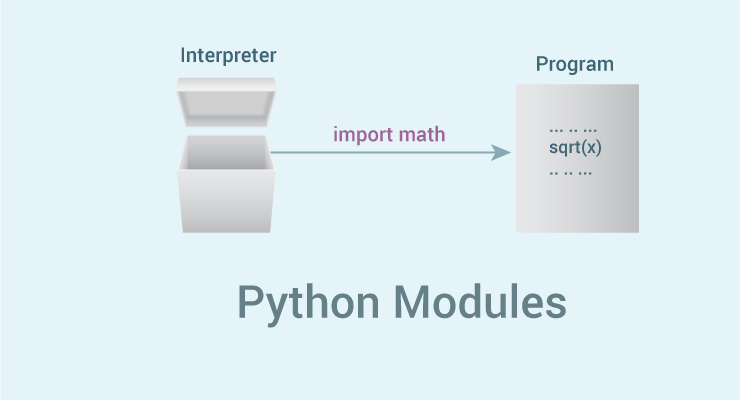
\includegraphics[width=0.50\textwidth]{figures/python_modules}}
	\caption{Python Modules}
	\label{Python Modules}
\end{figure}
\vspace{\baselineskip}

\noindent Modules\par

\vspace{\baselineskip}
\noindent Jika Anda berhenti dari juru bahasa Python dan memasukkannya lagi, definisi yang telah Anda buat (fungsi dan variabel) hilang. Oleh karena itu, jika Anda ingin menulis program yang agak lama, sebaiknya Anda menggunakan editor teks untuk menyiapkan masukan bagi penerjemah dan menjalankannya dengan file itu sebagai masukan. Ini dikenal dengan membuat skrip.\par
\vspace{\baselineskip}
\noindent Seiring program Anda semakin lama, Anda mungkin ingin membaginya menjadi beberapa file untuk memudahkan perawatan. Anda mungkin juga ingin menggunakan fungsi praktis yang telah Anda tulis di beberapa program tanpa menyalin definisinya ke dalam setiap program.\par
\vspace{\baselineskip}
\noindent Untuk mendukung ini, Python memiliki cara untuk menempatkan definisi dalam file dan menggunakannya dalam naskah atau dalam contoh juru bahasa interaktif. File seperti itu disebut modul; definisi dari modul dapat diimpor ke modul lain atau masuk ke modul utama (kumpulan variabel yang Anda akses ke dalam naskah yang dieksekusi di tingkat atas dan dalam mode kalkulator).\par

\vspace{\baselineskip}
\noindent Modul adalah file yang berisi definisi dan pernyataan Python. Nama file adalah nama modul dengan akhiran .py ditambahkan. Dalam sebuah modul, nama modul (sebagai string) tersedia sebagai nilai dari variabel global $ \_ $ $ \_ $ name$ \_ $ $ \_ $ . Misalnya, gunakan editor teks favorit Anda untuk membuat file bernama fibo.py di direktori saat ini dengan konten berikut.\par
\vspace{\baselineskip}
\subsection {More on Modules}

\noindent Modul dapat berisi pernyataan eksekusi serta definisi fungsi.Pernyataan ini dimaksudkan untuk menginisialisasi modul. Mereka dieksekusi hanya untuk pertama kalinya nama modul ditemukan dalam sebuah pernyataan impor. [1] (Mereka juga dijalankan jika file dijalankan sebagai skrip.)\par

\vspace{\baselineskip}
\noindent Setiap modul memiliki tabel simbol pribadinya, yang digunakan sebagai tabel simbol global oleh semua fungsi yang didefinisikan dalam modul.Dengan demikian, penulis modul dapat menggunakan variabel global dalam modul tanpa mengkhawatirkan bentrokan kecelakaan dengan variabel global pengguna.\par

\vspace{\baselineskip}
\noindent Di sisi lain, jika Anda tahu apa yang Anda lakukan, Anda dapat menyentuh variabel global modul dengan notasi yang sama yang digunakan untuk merujuk pada fungsinya, nama modname.itemname.\par

\vspace{\baselineskip}
\noindent Modul bisa mengimpor modul lainnya. Sudah menjadi kebiasaan tapi tidak diharuskan untuk menempatkan semua pernyataan impor di awal modul (atau naskah, dalam hal ini). Nama modul yang diimpor ditempatkan di tabel simbol global modul pengimpor.\par


\vspace{\baselineskip}
\noindent Executing modules as scripts\par
\vspace{\baselineskip}
\noindent Saat Anda menjalankan modul Python dengan\par
\vspace{\baselineskip}
\noindent python fibo.py <arguments>\par

\vspace{\baselineskip}
\noindent Kode dalam modul akan dieksekusi, sama seperti jika Anda mengimpornya, tapi dengan $ \_ $ $ \_ $ name$ \_ $ $ \_ $  set ke "$ \_ $ $ \_ $ main$ \_ $ $ \_ $ ". Itu berarti bahwa dengan menambahkan kode ini di akhir modul Anda:\par

\vspace{\baselineskip}
\noindent if $ \_ $ $ \_ $ name$ \_ $ $ \_ $  == "$ \_ $ $ \_ $ main$ \_ $ $ \_ $ ":\par
\vspace{\baselineskip}
\noindent ~~~ import sys\par
\vspace{\baselineskip}
\noindent ~~~ fib(int(sys.argv[1]))\par

\vspace{\baselineskip}
\noindent Anda dapat membuat file tersebut dapat digunakan sebagai skrip dan juga modul yang dapat diimpor, karena kode yang mem-parsing baris perintah hanya berjalan jika modul dijalankan sebagai file "utama":\par


\vspace{\baselineskip}
\noindent $\$$  python fibo.py 50\par


\noindent 1 1 2 3 5 8 13 21 34\par

\vspace{\baselineskip}
\noindent Jika modul diimpor, kode tidak dijalankan:\par


\noindent >>>\par


\noindent >>> import fibo\par


\noindent >>>\par

\vspace{\baselineskip}
\noindent Hal ini sering digunakan untuk menyediakan antarmuka pengguna yang mudah digunakan ke modul, atau untuk tujuan pengujian (menjalankan modul saat skrip menjalankan test suite).\par


\vspace{\baselineskip}
\begin{itemize}
	\item The Module Search Path
\end{itemize}

\noindent Ketika sebuah modul bernama spam diimpor, penerjemah pertama-tama mencari modul built-in dengan nama itu. Jika tidak ditemukan, maka cari file bernama spam.py dalam daftar direktori yang diberikan oleh variabel sys.path. sys.path diinisialisasi dari lokasi ini:\par

\vspace{\baselineskip}
\noindent $\bullet$  Direktori berisi skrip masukan (atau direktori saat ini bila tidak ada file yang ditentukan).\par
\vspace{\baselineskip}
\noindent $\bullet$  PYTHONPATH (daftar nama direktori, dengan sintaks yang sama dengan variabel shell PATH).\par
\vspace{\baselineskip}
\noindent $\bullet$  Default yang tergantung pada instalasi.\par

\vspace{\baselineskip}
\noindent Setelah inisialisasi, program Python dapat memodifikasi sys.path. Direktori yang berisi skrip yang dijalankan ditempatkan di awal jalur pencarian, di depan jalur perpustakaan standar.\par  
\vspace{\baselineskip}
\noindent Ini berarti skrip di direktori itu akan dimuat alih-alih modul dengan nama yang sama di direktori perpustakaan. Ini adalah kesalahan kecuali penggantinya. Lihat bagian Modul Standar untuk informasi lebih lanjut.\par


\vspace{\baselineskip}
\noindent $``$ Compiled$"$  Python files\par


\noindent Untuk mempercepat pemuatan modul, Python menyimpan versi yang dikompilasi setiap modul di direktori $ \_ $ $ \_ $ pycache$ \_ $ $ \_ $  dengan nama module.version.pyc, di mana versi tersebut mengkodekan format file yang dikompilasi; Umumnya berisi nomor versi Python.\par
\vspace{\baselineskip} 
\noindent Sebagai contoh, dalam rilis CPython 3.3 versi terkompilasi dari spam.py akan di-cache sebagai $ \_ $ $ \_ $ pycache $ \_ $ $ \_ $  / spam.cpython-33.pyc. Konvensi penamaan ini memungkinkan modul yang dikompilasi dari berbagai rilis dan versi Python yang berbeda untuk hidup berdampingan. \par

\vspace{\baselineskip}
\noindent Python memeriksa tanggal modifikasi sumber dari versi yang dikompilasi untuk melihat apakah sudah ketinggalan zaman dan perlu dikompilasi ulang. Ini adalah proses yang benar-benar otomatis.\par  
\vspace{\baselineskip}
\noindent Selain itu, modul yang dikompilasi bersifat platform-independen, sehingga perpustakaan yang sama dapat dibagi antar sistem dengan arsitektur yang berbeda.\par  
\vspace{\baselineskip}
\noindent Python tidak memeriksa cache dalam dua situasi. Pertama, selalu mengkompilasi ulang dan tidak menyimpan hasilnya untuk modul yang dimuat langsung dari baris perintah.\par
\vspace{\baselineskip}  
\noindent Kedua, tidak memeriksa cache jika tidak ada modul sumber. Untuk mendukung distribusi non-source (dikompilasi saja), modul yang dikompilasi harus berada dalam direktori sumber, dan tidak boleh ada modul sumber.\par


\vspace{\baselineskip}
\subsection {Beberapa tip untuk para ahli:}
\vspace{\baselineskip}
\noindent $\bullet$  Anda dapat menggunakan switch -O atau -OO pada perintah Python untuk mengurangi ukuran modul yang dikompilasi. Sakelar -O menghapus pernyataan tegas, tombol -OO menghapus kedua pernyataan tegas dan string $ \_ $ $ \_ $ doc$ \_ $ $ \_ $ .\par
\vspace{\baselineskip} 
\noindent $\bullet$  Karena beberapa program mungkin bergantung pada ketersediaan ini, Anda sebaiknya hanya menggunakan opsi ini jika Anda tahu apa yang Anda lakukan. Modul "Dioptimalkan" memiliki pilihan dan biasanya lebih kecil. Rilis masa depan dapat mengubah efek pengoptimalan.\par

\vspace{\baselineskip}
\noindent $\bullet$  Program tidak berjalan lebih cepat saat dibaca dari file .pyc daripada saat dibaca dari file .py; Satu-satunya yang lebih cepat tentang file .pyc adalah kecepatan pengisiannya.\par

\vspace{\baselineskip}
\noindent $\bullet$  Compileall modul dapat membuat file .pyc untuk semua modul dalam sebuah direktori.\par

\vspace{\baselineskip}
\noindent $\bullet$  Ada lebih banyak rincian mengenai proses ini, termasuk bagan alir keputusan, dalam PEP 3147.\par


%Kelompok 1 D4 TI 3D
%Wahyu Maruti Adjie_1154034
%Muhammad Nur Ikhsan_1154087
%Emy Safitri_1154102
%Andi Ikram Maulana_1154065
%Ilman Mubarik Sidiq_1154114

\section{Phyton Modules} 
Modul memungkinkan Kita mengatur kode Python secara logis. Mengelompokkan kode terkait ke dalam modul membuat kode lebih mudah dipahami \& digunakan. Modul merupakan objek Python dengan atribut yang diberi nama semena-mena sehingga Kita bisa mengikat \& memberi referensi.
\subsection{Modul Phyton}
modul adalah file yang terdiri dari kode Python. Modul dapat mendefinisikan fungsi, kelas \& variabel. Modul juga bisa menyertakan kode runnable.
Kode Python untuk sebuah modul bernama aname biasanya berada pada sebuah file bernama aname.py. Berikut adalah contoh modul sederhana, support.py  
\begin{verbatim}
def print _  _  \$func{ par }:  
print "Hello : ", par  
 return  
The \$  \$import \$
\end{verbatim}
Kita dapat menggunakan file sumber Python apapun sebagai modul dengan mengeksekusi pernyataan impor di file sumber Python lainnya. Import memiliki sintaks berikut:  
  import module1[, module2[,... moduleN]  
Ketika seorang penafsir menemukan sebuah pernyataan impor, ia mengimpor modul jika modul tersebut ada di jalur pencarian. Jalur pencarian adalah daftar direktori yang ditafsirkan juru bahasa sebelum mengimpor modul. Misalnya, untuk mengimpor modul support.py, Kita perlu meletakkan perintah berikut di bagian atas skript - 
 \begin{verbatim}
#!/usr/bin/python 
Import module support 
import support 
#  \ Now you can call defined function that module as follows 
support.print_ func("Zara")
A = “aku”
B = “kamu”
C = a+b
Print(c)
\end{verbatim}

Modul hanya dimuat satu kali, berapa pun jumlahnya diimpor. Hal ini mencegah eksekusi modul terjadi berulang-ulang jika terjadi beberapa impor. 
The from...import 

Python dari pernyataan memungkinkan Anda mengimpor atribut tertentu dari modul ke dalam namespace saat ini. Dari ... impor memiliki sintaks berikut - 
from modname import name1[, name2[, ... nameN]] 
Misalnya, untuk mengimpor fungsi fibonacci dari modul fib, gunakan pernyataan berikut 
from fib import fibonacci 
Pernyataan ini tidak mengimpor seluruh modul fib ke dalam namespace saat ini; Itu hanya memperkenalkan item fibonacci dari modul fib ke dalam tabel simbol global modul pengimpor.  
The from...import  
Hal ini juga memungkinkan untuk mengimpor semua nama dari modul ke dalam namespace saat ini dengan menggunakan pernyataan impor berikut 
from modname import * 
Ini menyediakan cara mudah untuk mengimpor semua item dari modul ke dalam namespace saat ini; Namun, pernyataan ini harus digunakan dengan hemat.
Locating Modules
Saat mengimpor modul, juru bahasa Python mencari modul dalam urutan berikut - 
 bullet  Direktori saat ini. 
 bullet Jika modul tidak ditemukan, Python kemudian mencari setiap direktori di variabel shell  PYTHONPATH. 
 bullet Jika semuanya gagal, Python memeriksa jalur default. Di UNIX, jalur default ini   biasanya / usr / local / lib / python /. 
Jalur pencarian modul disimpan dalam sistem modul sys sebagai sys.pathvariable. Variabel sys.path berisi direktori saat ini, PYTHONPATH, \& default pengaturan instalasi.
The  PYTHONPATH  Variable:  
The PYTHONPATH adalah variabel lingkungan, yang terdiri dari daftar direktori. Sintaksis PYTHONPATH sama dengan variabel shell PATH. 
Berikut adalah PYTHONPATH khas dari sistem Windows: 
set PYTHONPATH=c: python20  \$lib;  
Dan berikut ini adalah PYTHONPATH khas dari sistem UNIX: 
  set PYTHONPATH=/usr/local/lib/python  
Namespaces \& Scoping  
Variabel adalah nama (identifiers) yang memetakan ke objek. Namespace adalah kamus dari nama variabel (kunci) \& objek yang sesuai (nilai).  
Pernyataan pada phyton yang dapat mengakses sebuah variable di dalam namespace local  dalam sebuah namespace global, jika variable local  variable global memiliki kesamaan pada namanya, maka variable global memiliki satu kesamaan pada namanya, maka variable local akan membayangi variable global. ada setiap fungsi tentu memiliki namespace lokalnya sendiri, metode kelas ini mengikuti suatu aturan perlingkupan yang sama dengan fungsi seperti biasanya. 

Phyton membuat tebakan terdidik tentang variable yang bersifat local atau global . ini tentu dapat mengasumsikan bahwa setiap variable yang diberi nilai dalam suatu fungsi merupakan variable local.

Oleh karenanya, untuk menetapkan sebuah nilai pada variable global dalam suatu fungsi, kita harus terlebih dahulu menggunakan pernyataan global. Pernyataan gloval VarName akan memberitahu pada phyton bahwa VarName merupakan Variabel global. Phyton akan berhenti mencari namespace local untuk variable tersebut.
Sebagai contohnya, kita mendefinisikan sebuah variable money in the global namespace.dalam fungsi tersebut, kita menetapkan money a value. Oleh karena itu, phyton mengasumsikan variable local moneyas. Namun, kami mengakses nilai variable local moneybefore yang mengaturnya, jadi UnboundLocalError adalah hasilnya, \& Uncommenting pernyataan global yang akan memperbaiki masalahnya.
 
\begin{verbatim}
#!/usr/bin/python  
Money = 2000  
 def AddMoney():  
#  \ Uncomment the following line to fix the code:  
#  \ global Money  
  Money = Money + 1  
  print Money  
  AddMoney() 
  print Money
 \end{verbatim}
The dir( ) Function  
Fungsi dir () built-in mengembalikan daftar string yang diurutkan yang berisi nama yang ditentukan oleh sebuah modul. 
Daftar berisi nama semua modul, variabel dan fungsi yang didefinisikan dalam modul. Berikut adalah contoh sederhana - 
\begin{verbatim}
#!/usr/bin/python 
 Import built-in module math  
 import math  
 content = dir(math) 
 print content 
\end{verbatim}
Di sini, variabel string khusus  \$  \_  \$ \$  \_  \$name \$  \_  \$ \$  \_  \$ adalah nama modul, \&  \$  \_  \$ \$  \_  \$file \$  \_  \$ \$  \_  \$ adalah nama file tempat modul dimuat. 
The \$  \$globals() \$  \$and \$  \$locals() \$  \$Functions  \$ - \$  
Fungsi global  \& penduduk lokal () dapat digunakan untuk mengembalikan nama di ruang nama global \& lokal tergantung pada lokasi dari tempat mereka dipanggil.  
Jika penduduk setempat () dipanggil dari dalam sebuah fungsi, maka semua nama yang dapat diakses secara lokal berasal dari fungsi itu. 
Jika globals () dipanggil dari dalam sebuah fungsi, maka akan mengembalikan semua nama yang dapat diakses secara global dari fungsi itu. 
Jenis kembalian dari kedua fungsi ini adalah kamus. Oleh karena itu, nama dapat diekstrak dengan menggunakan tombol () fungsi.
The \$  \$reload() \$  \$Function  
Saat modul diimpor ke dalam skrip, kode di bagian tingkat atas dari modul hanya akan dijalankan satu kali.  
Oleh karena itu, jika Anda ingin mengulang ulang kode tingkat atas dalam modul, Anda dapat menggunakan fungsi reload (). Fungsi reload () mengimpor modul yang sebelumnya diimpor lagi. Sintaks fungsi reload () adalah ini -  
reload(module \$  \_  \$name) 
Di sini, module \$  \_  \$name adalah nama modul yang ingin Anda muat ulang \& bukan string yang berisi nama modul. Misalnya, untuk me-reload modul hello, lakukan hal berikut -  
reload(hello) 
Packages in Python 
Paket adalah struktur direktori file hirarkis yang mendefinisikan satu lingkungan aplikasi Python yang terdiri dari modul \& subpackages dan sub-subpackages, \& seterusnya.  
Pertimbangkan sebuah file Pots.py yang tersedia di direktori Phone. File ini memiliki baris kode sumber berikut Cara yang sama, kita memiliki dua file lain yang memiliki fungsi berbeda dengan nama yang sama seperti di atas -  
Phone/Isdn.py file having function Isdn()  
Phone/G3.py \$  file having function G3() 
Now, create one more file   \_   \_  init  \_ \_  .py in \$Phone  \$directory   
Phone/  \_   \_  init  \_  \_  .py  
Untuk membuat semua fungsi Anda tersedia saat mengimpor Telepon, Anda harus memasukkan pernyataan impor secara eksplisit di    \_     \_  init   \_  \_  .py sebagai berikut - 
 from Pots import Pots 
 from Isdn import Isdn  
 from G3 import G3 Setelah Anda menambahkan baris ini ke \_  \_  init  \_  \_  .py, Anda memiliki semua kelas ini yang tersedia saat Anda mengimpor paket Telepon. 
Pada contoh di atas, kita telah mengambil contoh fungsi tunggal di setiap file, namun Anda dapat menyimpan beberapa fungsi dalam file Anda. Anda juga dapat menentukan kelas Python yang berbeda dalam file tersebut dan kemudian Anda dapat membuat paket Anda dari kelas tersebut.
Modules  
Jika Anda berhenti dari juru bahasa Python  memasukkannya lagi, definisi yang telah Anda buat fungsi  variabel hilang. Oleh karena itu, jika Anda ingin menulis program yang agak lama, sebaiknya Anda menggunakan editor teks untuk menyiapkan masukan bagi penerjemah dan menjalankannya dengan file itu sebagai masukan. Ini dikenal dengan membuat skrip. Seiring program Anda semakin lama, Anda mungkin ingin membaginya menjadi beberapa file untuk memudahkan perawatan. Anda mungkin juga ingin menggunakan fungsi praktis yang telah Anda tulis di beberapa program tanpa menyalin definisinya ke dalam setiap program.  
Untuk mendukung ini, Python memiliki cara untuk menempatkan definisi dalam file dan menggunakannya dalam naskah atau dalam contoh juru bahasa interaktif. File seperti itu disebut modul; definisi dari modul dapat di impor ke modul lain atau masuk ke modul utama (kumpulan variabel yang Anda akses ke dalam naskah yang dieksekusi di tingkat atas dan dalam mode kalkulator).  
Modul adalah file yang berisi definisi  pernyataan Python. Nama file adalah nama modul dengan akhiran .py ditambahkan. Dalam sebuah modul, nama modul (sebagai string) tersedia sebagai nilai dari variabel global. Misalnya, gunakan editor teks favorit Anda untuk membuat file bernama fibo.py di direktori saat ini dengan konten berikut.  
6.1. More on Modules 
Modul dapat berisi pernyataan eksekusi serta definisi fungsi. Pernyataan ini dimaksudkan untuk menginisialisasi modul. Mereka dieksekusi hanya untuk pertama kalinya nama modul ditemukan dalam sebuah pernyataan impor. [1] (Mereka juga dijalankan jika file dijalankan sebagai skrip.)  
Setiap modul memiliki tabel simbol pribadinya, yang digunakan sebagai tabel simbol global oleh semua fungsi yang didefinisikan dalam modul. Dengan demikian, penulis modul dapat menggunakan variabel global dalam modul tanpa mengkhawatirkan bentrokan kecelakaan dengan variabel global pengguna. Di sisi lain, jika kita tahu apa yang kita lakukan, kita dapat menyentuh variabel global modul dengan notasi yang sama yang digunakan untuk merujuk pada fungsinya, nama modname.itemname. 
Modul bisa mengimpor modul lainnya. Sudah menjadi kebiasaan tapi tidak diharuskan untuk menempatkan semua pernyataan impor di awal modul (atau naskah, dalam hal ini). Nama modul yang diimpor ditempatkan di tabel simbol global modul pengimpor.  
6.1.1. Executing modules as scripts  
Saat Anda menjalankan modul Python dengan  
python fibo.py <arguments>  

Kode dalam modul akan dieksekusi, sama seperti jika kita mengimpornya, tapi dengan    \_     \_  name   \_     \_   set ke    \_     \_  main   \_     \_  . Itu berarti bahwa dengan menambahkan kode ini di akhir modul Anda: 
if    \_     \_  name   \_     \_   ==    \_     \_  main   \_     \_  :  

~~~ import sys 
~~~ fib(int(sys.argv[1])) 
Kita dapat membuat file tersebut dapat digunakan sebagai skrip dan juga modul yang dapat diimpor, karena kode yang mem-parsing baris perintah hanya berjalan jika modul dijalankan sebagai file.  
   \$   python fibo.py 50 t 
1 1 2 3 5 8 13 21 34  
Jika modul diimpor, kode tidak dijalankan:  
>>>  
>>> import fibo  
>>>  
Hal ini sering digunakan untuk menyediakan antarmuka pengguna yang mudah digunakan ke modul, atau untuk tujuan pengujian (menjalankan modul saat skrip menjalankan test suite). 
6.1.2. The Module Search Path 
Ketika sebuah modul bernama spam diimpor, penerjemah pertama-tama mencari modul built-in dengan nama itu. Jika tidak ditemukan, maka cari file bernama spam.py dalam daftar direktori yang diberikan oleh variabel sys.path. sys.path diinisialisasi dari lokasi ini:  
Direktori berisi skrip masukan (atau direktori saat ini bila tidak ada file yang ditentukan).  
PYTHONPATH (daftar nama direktori, dengan sintaks yang sama dengan variabel shell PATH).  
Default yang tergantung pada instalasi. 
Setelah inisialisasi, program Python dapat memodifikasi sys.path. Direktori yang berisi skrip yang dijalankan ditempatkan di awal jalur pencarian, di depan jalur perpustakaan standar. Ini berarti skrip di direktori itu akan dimuat alih-alih modul dengan nama yang sama di direktori perpustakaan. Ini adalah kesalahan kecuali penggantinya. Lihat bagian Modul Standar untuk informasi lebih lanjut.  

6.1.3.   " Compiled  "  Python files  
Untuk mempercepat pemuatan modul, Python menyimpan versi yang dikompilasi setiap modul di direktori  pycache    dengan nama module.version.pyc, di mana versi tersebut mengkodekan format file yang dikompilasi; Umumnya berisi nomor versi Python. Sebagai contoh, dalam rilis CPython 3.3 versi terkompilasi dari spam.py akan di-cache sebagai  pycache   spam.cpython-33.pyc. Konvensi penamaan ini memungkinkan modul yang dikompilasi dari berbagai rilis dan versi Python yang berbeda untuk hidup berdampingan.  
Python memeriksa tanggal modifikasi sumber dari versi yang dikompilasi untuk melihat apakah sudah ketinggalan zaman dan perlu dikompilasi ulang. Ini adalah proses yang benar-benar otomatis. Selain itu, modul yang dikompilasi bersifat platform-independen, sehingga perpustakaan yang sama dapat dibagi antar sistem dengan arsitektur yang berbeda. Python tidak memeriksa cache dalam dua situasi. Pertama, selalu mengkompilasi ulang dan tidak menyimpan hasilnya untuk modul yang dimuat langsung dari baris perintah. Kedua, tidak memeriksa cache jika tidak ada modul sumber. Untuk mendukung distribusi non-source (dikompilasi saja), modul yang dikompilasi harus berada dalam direktori sumber, dan tidak boleh ada modul sumber. 
Beberapa tip untuk para ahli:  
 Anda dapat menggunakan switch -O atau -OO pada perintah Python untuk mengurangi ukuran modul yang dikompilasi. Sakelar -O menghapus pernyataan tegas, tombol -OO menghapus kedua pernyataan tegas dan string doc  . Karena beberapa program mungkin bergantung pada ketersediaan ini, Anda sebaiknya hanya menggunakan opsi ini jika Anda tahu apa yang Anda lakukan. Modul "Dioptimalkan" memiliki pilihan dan biasanya lebih kecil. Rilis masa depan dapat mengubah efek pengoptimalan. 
  Program tidak berjalan lebih cepat saat dibaca dari file .pyc daripada saat dibaca dari file .py; Satu-satunya yang lebih cepat tentang file .pyc adalah kecepatan pengisiannya.  
  Compileall modul dapat membuat file .pyc untuk semua modul dalam sebuah direktori.  
  Kita lebih banyak rincian mengenai proses ini, termasuk bagan alir keputusan, dalam PEP 3147. 


6.1.3.   Compiled   Python files  
Untuk mempercepat pemuatan modul, Python menyimpan versi yang dikompilasi setiap modul di direktori    \_     \_  pycache   \_     \_   dengan nama module.version.pyc, di mana versi tersebut mengkodekan format file yang dikompilasi; Umumnya berisi nomor versi Python. Sebagai contoh, dalam rilis CPython 3.3 versi terkompilasi dari spam.py akan di-cache sebagai    \_     \_  pycache    \_     \_   / spam.cpython-33.pyc. Konvensi penamaan ini memungkinkan modul yang dikompilasi dari berbagai rilis dan versi Python yang berbeda untuk hidup berdampingan.  
Python memeriksa tanggal modifikasi sumber dari versi yang dikompilasi untuk melihat apakah sudah ketinggalan zaman dan perlu dikompilasi ulang. Ini adalah proses yang benar-benar otomatis. Selain itu, modul yang dikompilasi bersifat platform-independen, sehingga perpustakaan yang sama dapat dibagi antar sistem dengan arsitektur yang berbeda. Python tidak memeriksa cache dalam dua situasi. Pertama, selalu mengkompilasi ulang dan tidak menyimpan hasilnya untuk modul yang dimuat langsung dari baris perintah. Kedua, tidak memeriksa cache jika tidak ada modul sumber. Untuk mendukung distribusi non-source (dikompilasi saja), modul yang dikompilasi harus berada dalam direktori sumber, dan tidak boleh ada modul sumber. 
Beberapa tip untuk para ahli:  
 Anda dapat menggunakan switch -O atau -OO pada perintah Python untuk mengurangi ukuran modul yang dikompilasi. Sakelar -O menghapus pernyataan tegas, tombol -OO menghapus kedua pernyataan tegas dan string    \_     \_  doc   \_     \_  . Karena beberapa program mungkin bergantung pada ketersediaan ini, Anda sebaiknya hanya menggunakan opsi ini jika Anda tahu apa yang Anda lakukan. Modul Dioptimalkan memiliki pilihan dan biasanya lebih kecil. Rilis masa depan dapat mengubah efek pengoptimalan. 

\section{modul}

Modul memungkinkan Anda mengatur kode Python secara logis. Mengelompokkan kode terkait ke dalam suatu modul membuat kode lebih cepat dipahami dan digunakan. Modul ini merupakan objek Python dengan atribut yang diberi nama sewenang-wenang sehingga Anda bisa mengikat dan memberi referensi.
Cukup, modul merupakan file yang terdiri dari kode Python. Modul bisa mendefinisikan fungsi, kelas dan variabel. Modul juga dapat menyertakan kode runnable.
Example
Kode Python untuk sebuah modul yang di beri nama aname biasanya berada pada sebuah file bernama aname.py. 

\subsection{import}
Ketika penafsir menemukan sebuah pernyataan impor, ia mengimpor modul apabila modul tersebut berada di jalur pencarian. Jalur pencarian merupakan daftar direktori yang ditafsirkan juru bahasa sebelum mengimpor modul. Misalnya, untuk mengimpor modul support.py, Anda perlu meletakkan perintah berikut di bagian atas skrip - 
 
\subsection{buat modul}Modul hanya dimuat satu kali, berapa pun jumlahnya diimpor. Hal ini mencegah eksekusi modul terjadi berulang-ulang jika terjadi beberapa impor.
 

\subsection{PYTHONPATH} 
The PYTHONPATH merupakan variabel lingkungan, yang terdiri dari daftar direktori. Sintaksis PYTHONPATH sama dengan variabel shell PATH. 
Berikut adalah PYTHONPATH khas dari sistem Windows:
 
\subsection{variabel}
Pernyataan global VarName memberitahu Python bahwa VarName merupakan variabel global. Python berhenti mencari namespace lokal untuk variabel tersebut. 
Sebagai contoh, kita mendefinisikan sebuah variabel Money in the global namespace. Dalam fungsi Money, kita menetapkan Money a value, oleh karena itu Python mengasumsikan variabel lokal Moneyas. Namun, kami mengakses nilai variabel lokal Moneybefore yang mengaturnya, jadi UnboundLocalError merupakan hasilnya. Uncommenting pernyataan global memperbaiki masalahnya.
 
\subsection{the dir Function}
Fungsi dir built-in mengembalikan daftar string yang diurutkan yang berisi nama yang ditentukan oleh sebuah modul.
Daftar berisi nama semua modul, variabel dan fungsi yang didefinisikan dalam modul. Berikut merupakan contoh sederhana - 

\subsection{paket}
Paket merupakan struktur direktori file hirarkis yang mendefinisikan satu lingkungan aplikasi Python yang terdiri dari modul dan subpackages dan sub-subpackages, dan seterusnya.
Pertimbangkan sebuah file Pots.py yang tersedia di direktori Phone. File ini memiliki baris kode sumber berikut -

Jika Anda berhenti dari juru bahasa Python dan memasukkannya lagi, definisi yang telah Anda buat (fungsi dan variabel) hilang. Oleh karena itu, jika Anda ingin menulis program yang agak lama, sebaiknya Anda menggunakan editor teks untuk menyiapkan masukan bagi penerjemah dan menjalankannya dengan file itu sebagai masukan. Ini dikenal dengan membuat skrip. Seiring program Anda semakin lama, Anda mungkin ingin membaginya menjadi beberapa file untuk memudahkan perawatan. Anda mungkin juga ingin menggunakan fungsi praktis yang telah Anda tulis di beberapa program tanpa menyalin definisinya ke dalam setiap program.
Untuk mendukung ini, Python memiliki cara untuk menempatkan definisi dalam file dan menggunakannya dalam naskah atau dalam contoh juru bahasa interaktif. File seperti itu disebut modul; definisi dari modul dapat diimpor ke modul lain atau masuk ke modul utama (kumpulan variabel yang Anda akses ke dalam naskah yang dieksekusi di tingkat atas dan dalam mode kalkulator).
Modul merupakan file yang berisi definisi dan pernyataan Python. Nama file merupakan nama modul dengan akhiran .py ditambahkan. Dalam sebuah modul, nama modul (sebagai string) tersedia sebagai nilai dari variabel global. Misalnya, gunakan editor teks favorit Anda untuk membuat file bernama fibo.py di direktori saat ini dengan konten berikut. 

Modul dapat berisi pernyataan eksekusi serta definisi fungsi. Pernyataan ini dimaksudkan untuk menginisialisasi modul. Mereka dieksekusi hanya untuk pertama kalinya nama modul ditemukan dalam sebuah pernyataan impor. [1] (Mereka juga dijalankan jika file dijalankan sebagai skrip.
Setiap modul memiliki tabel simbol pribadinya, yang digunakan sebagai tabel simbol global oleh semua fungsi yang didefinisikan dalam modul. Dengan demikian, penulis modul dapat menggunakan variabel global dalam modul tanpa mengkhawatirkan bentrokan kecelakaan dengan variabel global pengguna. Di sisi lain, jika Anda tahu apa yang Anda lakukan, Anda dapat menyentuh variabel global modul dengan notasi yang sama yang digunakan untuk merujuk pada fungsinya, nama modname.itemname.
Modul bisa mengimpor modul lainnya. Sudah menjadi kebiasaan tapi tidak diharuskan untuk menempatkan semua pernyataan impor di awal modul (atau naskah, dalam hal ini). Nama modul yang diimpor ditempatkan di tabel simbol global modul pengimpor.


\chapter{Files I/O}
%


\begin{figure}[ht]
	\centerline{
\includegraphics[width=0.60\textwidth]{Gambar/dapi7.jpg}}
	\caption{File I/O}
	\label{File I/O}
\end{figure}



\section {Pengertian }
\subsection {Python File I/O}

Unit~input~adalah (masukan) suatu  data yang berbentuk documet bait itu data data foto, data data hurup ataupun data tanggal ke dalam sebuah system yang  terkomputerisasi.  unit output (keluaran) biasanya digunakan untuk menampilkan data, atau dengan kata lain untuk menangkap data yang telah diinputkan terlebih dahulu dalam sebuah penyimpanan media elektronic , contohnya data yang akan ditampilkan pada layar monitor atau printer. \par
I/O Input/Ouput Read [IOR] dan untuk tulis I/O Input/Output Write [IOW]. File adalah lokasi bernama pada disk untuk menyimpan informasi terkait. Ini digunakan untuk menyimpan data secara permanen dalam memori non-volatile (misalnya hard disk). Karena, random access memory (RAM) bersifat volatile sehingga kehilangan datanya saat komputer dimatikan, kita menggunakan file untuk penggunaan data masa depan. Bila kita ingin membaca dari atau menulis ke file kita perlu membukanya terlebih dahulu. Bila sudah selesai, perlu ditutup, agar sumber yang diikat dengan file tersebut dibebaskan.Oleh karena itu, dengan Python, sebuah operasi file berlangsung dengan urutan sebagai berikut. \par
\vspace{12pt}
\noindent 

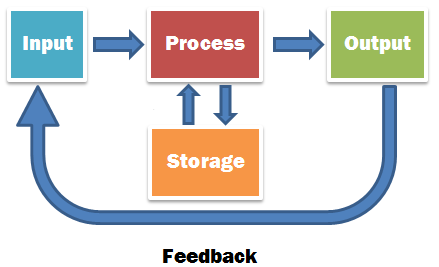
\includegraphics[width=15cm,height=7cm]{Gambar/dapi8.jpg}
\begin{equation}Python File I/O\end{equation}


\begin{enumerate}
	


	\item Buka file 

	\item Membaca atau menulis (melakukan operasi) 
	\item Tutup file tersebu 
	\end {enumerate}
\vspace{12pt}
\vspace{12pt}
\vspace{12pt}
\noindent 
Membuka sebuah file \par
\noindent 
Python memiliki built-in function open () untuk membuka file. Fungsi ini mengembalikan objek file, juga disebut handle, karena digunakan untuk membaca atau memodifikasi file yang sesuai. \par
\vspace{12pt}
\noindent 

\begin{verbatim}

>>>~f~=~open("test.txt")    
 $  \#  $ open file in current directory \par
\noindent 
>>>~f = open("C:/Python33/README.txt")  
 $  \#  $ specifying full path \par
\vspace{12pt}

\end{verbatim}

Kita bisa menentukan mode saat membuka file. Dalam mode, kami menentukan apakah kita ingin membaca 'r', menulis 'w' atau menambahkan 'a' ke file. Kita juga menentukan apakah kita ingin membuka file dalam mode teks atau mode biner. Defaultnya adalah membaca dalam mode teks. Dalam mode ini, kita mendapatkan string saat membaca dari file. Di sisi lain, mode biner mengembalikan byte dan ini adalah mode yang akan digunakan saat berhadapan dengan file non-teks seperti file gambar atau exe. \par
\vspace{12pt}
\vspace{12pt}
\noindent 

\begin{enumerate}


\item 'r' \hspace*{0.5in}  \par
\noindent 
Buka file untuk dibaca. (default) \par
\vspace{12pt}
\noindent 

\item 'w' \hspace*{0.5in}  \par
\noindent 
Buka file untuk menulis. Membuat file baru jika tidak ada atau memotong file jika file tersebut ada. \par
\vspace{12pt}
\noindent 

\item 'x' \hspace*{0.5in}  \par
\noindent 
Buka file untuk pembuatan eksklusif. Jika file sudah ada, operasi gagal \par
\vspace{12pt}
\noindent 

\item 'a' \hspace*{0.5in}  \par
\noindent 
Buka untuk menambahkan di akhir file tanpa memotongnya. Membuat file baru jika tidak ada. \par
\vspace{12pt}
\noindent 

\item 't' \hspace*{0.5in}  \par
\noindent 
Buka dalam mode teks. (default) \par
\vspace{12pt}
\noindent 

\item 'b' \par
\noindent 
Buka dalam mode biner. \par
\vspace{12pt}
\noindent 
\item '+' \par
\noindent 
Buka file untuk mengupdate (membaca dan menulis) \par
\vspace{12pt}
\noindent 

\end {enumerate}

\begin{verbatim}

f~=~open("test.txt")~~~   
 $  \#  $ equivalent to 'r' or 'rt' \par
\noindent 
f~= open("test.txt",'w')  
 $  \#  $ write in text mode \par
\noindent 
f = open("img.bmp",'r+b') 
 $  \#  $ read and write in binary mode \par
\vspace{12pt}
\noindent 

\end{verbatim}

Tidak seperti bahasa lain, karakter 'a' tidak menyiratkan angka 97 sampai dikodekan menggunakan ASCII (atau pengkodean setara lainnya). Apalagi, pengkodean default bergantung pada platform. Di jendela, itu adalah 'cp1252' tapi 'utf-8' di Linux. Jadi, kita juga tidak harus bergantung pada pengkodean default atau kode kita akan berperilaku berbeda di berbagai platform. Oleh karena itu, ketika bekerja dengan file dalam mode teks, sangat disarankan untuk menentukan jenis pengkodean. \par
\vspace{12pt}
\noindent 
f = open("test.txt",mode = 'r',encoding = 'utf-8') \par
\vspace{12pt}
\noindent 
\section{Menutup sebuah File}
Ketika kita selesai dengan operasi ke file, kita perlu menutupinya dengan benar. Menutup file akan membebaskan sumber daya yang terkait dengan file dan dilakukan dengan menggunakan metode close (). Python memiliki pengumpul sampah untuk membersihkan benda yang tidak difermentasi tapi, kita tidak boleh bergantung padanya untuk menutup file. \par
\noindent 
f = open("test.txt",encoding = 'utf-8') \par
\noindent 
$  \#  $ perform file operations \par
\noindent 
f.close() \par
\vspace{12pt}
\noindent 
Metode ini tidak sepenuhnya aman. Jika pengecualian terjadi saat kita melakukan operasi dengan file, kode keluar tanpa menutup file. Cara yang lebih aman adalah dengan menggunakan try ... akhirnya blok. \par
\vspace{12pt}
\noindent 
try: \par
\noindent 
~~ f = open("test.txt",encoding = 'utf-8') \par
\noindent 
~~  $  \#  $ perform file operations \par
\noindent 
finally: \par
\noindent 
~~ f.close() \par
\vspace{12pt}
Dengan cara ini, kita dijamin bahwa file tersebut benar tertutup bahkan jika pengecualian dinaikkan, menyebabkan aliran program berhenti. Cara terbaik untuk melakukannya adalah dengan menggunakan pernyataan. Ini memastikan file ditutup saat blok di dalam dengan keluar. Kita tidak perlu secara eksplisit memanggil metode close (). Hal itu dilakukan secara internal. \par
\vspace{12pt}
\noindent 
with open("test.txt",encoding = 'utf-8') as f: \par
\noindent 
~~  $  \#  $ perform file operations \par
\vspace{12pt}
\noindent 
\section{Menulis ke File}
Untuk menulis ke file kita perlu membukanya dalam mode write 'w', tambahkan 'a' atau exclusive creation 'x'. Kita harus berhati-hati dengan mode 'w' karena akan menimpa file jika sudah ada. Semua data sebelumnya terhapus. Menulis string atau urutan byte (untuk file biner) dilakukan dengan menggunakan metode write (). Metode ini mengembalikan jumlah karakter yang ditulis ke file. \par
\vspace{12pt}
\noindent 
with open("test.txt",'w',encoding = 'utf-8') as f: \par
\noindent 
~~ f.write("my first file $  \setminus  $n") \par
\noindent 
~~ f.write("This file $  \setminus  $n $  \setminus  $n") \par
\noindent 
~~ f.write("contains three lines $  \setminus  $n") \par
\vspace{12pt}
Program ini akan membuat file baru bernama 'test.txt' jika tidak ada. Jika memang ada, itu akan ditimpa. Kita harus menyertakan karakter newline sendiri untuk membedakan garis yang berbeda. \par
\vspace{12pt}
\noindent 
{\fontsize{14pt}{14pt}\selectfont \textbf{Membaca Dari File} \\} \par
\vspace{12pt}
Untuk membaca isi sebuah file, kita harus membuka file dalam mode baca. Ada berbagai metode yang tersedia untuk tujuan ini. Kita bisa menggunakan metode read (size) untuk membaca dalam jumlah ukuran data. Jika parameter ukuran tidak ditentukan, bunyinya dan kembali ke akhir file. \par
\vspace{12pt}
\vspace{12pt}
\noindent 
>>> f = open("test.txt",'r',encoding = 'utf-8') \par
\noindent 
>>>~f.read(4)~~   $  \#  $ read the first 4 data \par
\noindent 
'This' \par
\vspace{12pt}
\noindent 
>>>~f.read(4)~~   $  \#  $ read the next 4 data \par
\noindent 
' is ' \par
\vspace{12pt}
\noindent 
>>>~f.read()~~~   $  \#  $ read in the rest till end of file \par
\noindent 
'my first file $  \setminus  $nThis file $  \setminus  $ncontains three lines $  \setminus  $n' \par
\vspace{12pt}
\noindent 
>>>~f.read()   $  \#  $ further reading returns empty sting \par
\vspace{12pt}
Kita dapat melihat, metode read () mengembalikan baris baru sebagai ' $  \setminus  $ n'. Begitu akhir file tercapai, kita mendapatkan string kosong untuk dibaca lebih lanjut. Kita bisa mengubah kursor file kita saat ini (posisi) dengan menggunakan metode seek (). Demikian pula metode tell () mengembalikan posisi kita saat ini (dalam jumlah byte). \par
\vspace{12pt}
\noindent 
>>>~f.tell()~~   $  \#  $ get the current file position \par
\noindent 
56 \par
\vspace{12pt}
\noindent 
>>>~f.seek(0)~   $  \#  $ bring file cursor to initial position \par
\noindent 
0 \par
\vspace{12pt}
\noindent 
>>>~print(f.read())   $  \#  $ read the entire file \par
\noindent 
This is my first file \par
\noindent 
This file \par
\noindent 
contains three lines \par
\vspace{12pt}
\vspace{12pt}
\noindent 
Kita bisa membaca file line-by-line menggunakan for loop. Ini efisien dan cepat. \par
\vspace{12pt}
\noindent 
>>> for line in f: \par
\noindent 
...~~~~ print(line, end = '') \par
\noindent 
... \par
\noindent 
This is my first file \par
\noindent 
This file \par
\noindent 
contains three lines \par
Baris dalam file itu sendiri memiliki karakter baris baru ' $  \setminus  $ n'. Terlebih lagi, print () parameter akhir untuk menghindari dua baris baru saat mencetak. Sebagai alternatif, kita dapat menggunakan metode readline () untuk membaca setiap baris file. Metode ini membaca sebuah file sampai newline, termasuk newline character. \par
\vspace{12pt}
\noindent 
>>> f.readline() \par
\noindent 
'This is my first file $  \setminus  $n' \par
\vspace{12pt}
\noindent 
>>> f.readline() \par
\noindent 
'This file $  \setminus  $n' \par
\vspace{12pt}
\noindent 
>>> f.readline() \par
\noindent 
'contains three lines $  \setminus  $n' \par
\vspace{12pt}
\noindent 
>>> f.readline() \par
\noindent 
'' \par
\vspace{12pt}
Terakhir, metode readlines () mengembalikan daftar baris yang tersisa dari keseluruhan file. Semua metode membaca ini mengembalikan nilai kosong saat akhir file (EOF) tercapai. \par
\vspace{12pt}
\noindent 
>>> f.readlines() \par
\noindent 
['This is my first file $  \setminus  $n', 'This file $  \setminus  $n', 'contains three lines $  \setminus  $n'] \par
\vspace{12pt}
\vspace{12pt}
\noindent 
{\fontsize{14pt}{14pt}\selectfont \textbf{Metode Berkas Python} \\} \par
\vspace{12pt}
Ada berbagai metode yang tersedia dengan objek file. Beberapa di antaranya telah digunakan pada contoh di atas. Berikut adalah daftar lengkap metode dalam mode teks dengan deskripsi singkat. Atribut Objek file Setelah file dibuka dan Anda memiliki satu file objek, Anda bisa mendapatkan berbagai informasi yang berkaitan dengan file tersebut. Berikut adalah daftar semua atribut yang terkait dengan objek file: \par
\vspace{12pt}
\vspace{12pt}
\vspace{12pt}
\noindent 
$  \#  $!/usr/bin/python \par
\vspace{12pt}
\noindent 
$  \#  $ Open a file \par
\noindent 
fo = open("foo.txt", "wb") \par
\noindent 
print "Name of the file: ", fo.name \par
\noindent 
print "Closed or not : ", fo.closed \par
\noindent 
print "Opening mode : ", fo.mode \par
\noindent 
print "Softspace flag : ", fo.softspace \par
\vspace{12pt}
\noindent 
Membaca dan Menulis File \par
\vspace{12pt}
Objek file menyediakan seperangkat metode akses untuk membuat hidup kita lebih mudah. Kita akan melihat bagaimana menggunakan metode read () dan write () untuk membaca dan menulis file. Metode tulis () Metode write () menulis string apapun ke file yang terbuka. Penting untuk dicatat bahwa string Python dapat memiliki data biner dan bukan hanya teks. Metode write () tidak menambahkan karakter baris baru (' $  \setminus  $ n') ke akhir string - \par
\noindent 
Sintaksis \par
\vspace{12pt}
\noindent 
$  \#  $!/usr/bin/python \par
\vspace{12pt}
\noindent 
$  \#  $ Open a file \par
\noindent 
fo = open("foo.txt", "wb") \par
\noindent 
fo.write( "Python is a great language. $  \setminus  $nYeah its great!! $  \setminus  $n"); \par
\vspace{12pt}
\noindent 
$  \#  $ Close opend file \par
\noindent 
fo.close() \par
\noindent 
$  \#  $!/usr/bin/python \par
\vspace{12pt}
\noindent 
$  \#  $ Open a file \par
\noindent 
fo = open("foo.txt", "r+") \par
\noindent 
str = fo.read(10); \par
\noindent 
print "Read String is : ", str \par
\vspace{12pt}
\noindent 
$  \#  $ Close opend file \par
\noindent 
fo.close() \par
\vspace{12pt}
\noindent 
Read~String is :  Python is \par
\vspace{12pt}
\noindent 
$  \#  $!/usr/bin/python \par
\vspace{12pt}
\noindent 
$  \#  $ Open a file \par
\noindent 
fo = open("foo.txt", "r+") \par
\noindent 
str = fo.read(10); \par
\noindent 
print "Read String is : ", str \par
\vspace{12pt}
\noindent 
$  \#  $ Check current position \par
\noindent 
position = fo.tell(); \par
\noindent 
print "Current file position : ", position \par
\vspace{12pt}
\noindent 
$  \#  $ Reposition pointer at the beginning once again \par
\noindent 
position = fo.seek(0, 0); \par
\noindent 
str = fo.read(10); \par
\noindent 
print "Again read String is : ", str \par
\noindent 
$  \#  $ Close opend file \par
\noindent 
fo.close() \par
\vspace{12pt}
\noindent 
Read~String is :  Python is \par
\noindent 
Current~file position :  10 \par
\noindent 
Again~read String is :  Python is \par
\vspace{12pt}
\noindent 
os.rename(current $  \_  $file $  \_  $name, new $  \_  $file $  \_  $name) \par
\vspace{12pt}
\noindent 
$  \#  $!/usr/bin/python \par
\noindent 
import os \par
\vspace{12pt}
\noindent 
$  \#  $ Rename a file from test1.txt to test2.txt \par
\noindent 
os.rename( "test1.txt", "test2.txt" ) \par
\vspace{12pt}
\noindent 
$  \#  $!/usr/bin/python \par
\noindent 
import os \par
\vspace{12pt}
\noindent 
$  \#  $ Delete file test2.txt \par
\noindent 
os.remove("text2.txt") \par
\vspace{12pt}
\noindent 
os.mkdir("newdir") \par
\vspace{12pt}
\noindent 
$  \#  $!/usr/bin/python \par
\noindent 
import os \par
\vspace{12pt}
\noindent 
$  \#  $ Create a directory "test" \par
\noindent 
os.mkdir("test") \par
\vspace{12pt}
\noindent 
$  \#  $!/usr/bin/python \par
\noindent 
import os \par
\vspace{12pt}
\noindent 
$  \#  $ Changing a directory to "/home/newdir" \par
\noindent 
os.chdir("/home/newdir") \par
\vspace{12pt}
\noindent 
$  \#  $!/usr/bin/python \par
\noindent 
import os \par
\vspace{12pt}
\noindent 
$  \#  $ This would give location of the current directory \par
\noindent 
os.getcwd() \par
\vspace{12pt}
\noindent 
$  \#  $!/usr/bin/python \par
\noindent 
import os \par
\vspace{12pt}
\noindent 
$  \#  $~This~would  remove "/tmp/test"  directory. \par
\noindent 
os.rmdir(~"/tmp/test"  ) \par
\vspace{12pt}
\vspace{12pt}
\noindent 
{\fontsize{14pt}{14pt}\selectfont \textbf{Membuka sebuah file} \\} \par
\vspace{12pt}
Untuk membuka file teks yang Anda gunakan, well, open () function. Sepertinya masuk akal. Anda melewatkan parameter tertentu untuk membuka () untuk memberitahukannya di mana file harus dibuka - 'r' untuk dibaca saja, 'w' untuk tulisan saja (jika ada file lama, akan dituliskan), 'a 'Untuk menambahkan (menambahkan sesuatu ke akhir file) dan' r + 'untuk membaca dan menulis. Tapi kurang bicara, mari kita buka file untuk membaca (Anda bisa melakukan ini dengan mode idle python Anda). Buka file teks biasa. Kami kemudian akan mencetak apa yang kita baca di dalam file: \par
\noindent 
Contoh Kode 1 - Membuka sebuah file \par
\vspace{12pt}
\noindent 
Openfile = open ('pathtofile', 'r') \par
\noindent 
Openfile.read () \par
\vspace{12pt}
Itu menarik. Anda akan melihat banyak simbol ' $  \setminus  $ n'. Ini merupakan baris baru (di mana Anda menekan enter untuk memulai baris baru). Teksnya benar-benar tidak diformat, tapi jika Anda melewati keluaran openfile.read () untuk mencetak (dengan mengetikkan print openfile.read ()) akan diformat dengan baik. Carilah dan Anda Temukan Apakah Anda mencoba mengetik di print openfile.read ()? Apakah itu gagal? Kemungkinan besar, dan alasannya adalah karena 'kursor' telah mengubah tempatnya. Kursor Kursor apa Nah, kursor yang sebenarnya tidak bisa kamu lihat, tapi tetap kursor. Kursor tak terlihat ini memberitahukan fungsi baca (dan banyak fungsi I / O lainnya) dari mana mulai. Untuk mengatur di mana kursor berada, Anda menggunakan fungsi seek (). Ini digunakan dalam bentuk seek (offset, dari mana). Mana yang opsional, dan menentukan mana yang harus dicari. Jika darimana 0, byte / huruf dihitung dari awal. Jika 1, byte dihitung dari posisi kursor saat ini. Jika 2, maka byte dihitung dari akhir file. Jika tidak ada yang diletakkan di sana, 0 diasumsikan. \par
\vspace{12pt}
\noindent 
Offset menggambarkan seberapa jauh dari mana kursor bergerak. sebagai contoh: \par
\vspace{12pt}
\noindent 
~~~ openfile.seek (45,0) akan memindahkan kursor ke 45 byte / huruf setelah permulaan file. \par
\noindent 
~~~ Openfile.seek (10,1) akan memindahkan kursor ke 10 byte / huruf setelah posisi kursor saat ini. \par
\noindent 
~~~ openfile.seek (-77,2) akan memindahkan kursor ke 77 byte / huruf sebelum akhir file (perhatikan - sebelum angka 77) \par
\vspace{12pt}
Cobalah sekarang juga. Gunakan openfile.seek () untuk pergi ke tempat manapun di file dan kemudian mencoba mengetik print openfile.read (). Ini akan dicetak dari tempat yang Anda inginkan. Tapi sadari bahwa openfile.read () memindahkan kursor ke akhir file - Anda harus mencari lagi. \par
\vspace{12pt}
\noindent 
{\fontsize{14pt}{14pt}\selectfont \textbf{Fungsi I / O Lainnya} \\} \par
\vspace{12pt}
Ada banyak fungsi lain yang membantu Anda dalam berurusan dengan file. Mereka memiliki banyak kegunaan yang memberdayakan Anda untuk berbuat lebih banyak, dan membuat hal-hal yang dapat Anda lakukan lebih mudah. Mari kita lihat kirim (), readline (), readlines (), tulis () dan close (). Kirim () mengembalikan tempat kursor berada dalam file. Tidak memiliki parameter, ketik saja (seperti contoh di bawah ini yang akan ditampilkan). Ini sangat berguna, untuk mengetahui apa yang Anda maksud, di mana letaknya, dan kontrol kursor yang sederhana. Untuk menggunakannya, ketik fileobjectname.tell () - dimana fileobjectname adalah nama dari file objek yang Anda buat saat Anda membuka file (di openfile = open ('pathtofile', 'r') nama objek file adalah openfile). Readline () membaca dari mana kursor sampai akhir baris. Ingat bahwa akhir baris bukan tepi layar Anda - garis berakhir saat Anda menekan enter untuk membuat baris baru. Ini berguna untuk hal-hal seperti membaca log peristiwa, atau mengalami sesuatu yang progresif untuk mengolahnya. Tidak ada parameter yang harus Anda lewati ke readline (), meskipun secara opsional Anda dapat memberi tahu jumlah maksimal byte / huruf untuk dibaca dengan meletakkan nomor di tanda kurung. Gunakan dengan fileobjectname.readline (). \par
Readlines () sama seperti readline (), namun readlines () membaca semua baris dari kursor dan seterusnya, dan mengembalikan sebuah daftar, dengan setiap elemen daftar memegang satu baris kode. Gunakan dengan fileobjectname.readlines (). Misalnya, jika Anda memiliki file teks: \par
\noindent 
Contoh Kode 2 - contoh file teks \par
\vspace{12pt}
\noindent 
Baris 1 \par
\vspace{12pt}
\noindent 
Baris 3 \par
\noindent 
Baris 4 \par
\vspace{12pt}
\noindent 
Baris 6 \par
\vspace{12pt}
Fungsi write (), menulis ke file. Bagaimana kamu menebak nya??? Ini menulis dari mana kursor berada, dan menimpa teks di depannya - seperti di MS Word, di mana Anda menekan 'insert' dan menulis di atas teks lama. Untuk memanfaatkan fungsi yang paling penting ini, letakkan string di antara tanda kurung untuk ditulis mis. fileobjectname.write ('ini adalah string'). \hspace*{0.5in} Dekat, Anda bisa mencari, menutup file sehingga Anda tidak dapat lagi membaca atau menulis sampai Anda membuka kembali lagi. Cukup sederhana Untuk menggunakan, Anda akan menulis fileobjectname.close (). Sederhana! Dengan mode siaga Python, buka file uji (atau buat yang baru ...) dan mainkan fungsi ini. Anda bisa melakukan penyuntingan teks yang sederhana (dan sangat merepotkan). \par
Mmm, acar Pickles, dengan Python, harus dimakan. Rasa mereka hanya untuk membiarkan pemrogram meninggalkan mereka di lemari es.Ok, hanya bercanda disana. Pickles, dengan Python, adalah objek yang disimpan ke sebuah file. Objek dalam kasus ini bisa berupa variabel, instance dari kelas, atau daftar, kamus, atau tupel. Hal lain juga bisa acar, tapi dengan batas. Objek kemudian dapat dipulihkan, atau tidak dicemari, nanti. Dengan kata lain, Anda 'menyimpan' benda Anda. Jadi bagaimana kita acar? Dengan fungsi dump (), yang ada di dalam modul acar - jadi pada awal program Anda, Anda harus menulis acar impor. Cukup sederhana Kemudian buka file kosong, dan gunakan pickle.dump () untuk menjatuhkan objek ke file itu. Mari kita coba itu: \par
\noindent 
Contoh Kode 3 - pickletest.py \par
\vspace{12pt}
\noindent 
$  \#  $ $  \#  $ $  \#  $ pickletest.py \par
\noindent 
$  \#  $ $  \#  $ $  \#  $ PICKLE AN OBJECT \par
\vspace{12pt}
\noindent 
$  \#  $ mengimpor modul acar \par
\noindent 
Acar impor \par
\vspace{12pt}
\noindent 
$  \#  $ Mari membuat sesuatu untuk menjadi acar \par
\noindent 
$  \#  $ Bagaimana dengan daftar? \par
\noindent 
picklelist = ['one', 2, 'three', 'four', 5, 'dapatkah kamu menghitung?'] \par
\vspace{12pt}
\noindent 
$  \#  $ Sekarang buat file \par
\noindent 
$  \#  $ ganti nama file dengan file yang ingin Anda buat \par
\noindent 
File = open ('filename', 'w') \par
\vspace{12pt}
\noindent 
$  \#  $ Sekarang mari kita pilih picklelist \par
\noindent 
pickle.dump (picklelist, file) \par
\vspace{12pt}
\noindent 
$  \#  $ Tutup file, dan pengawetan Anda sudah selesai \par
\noindent 
file.close () \par
\vspace{12pt}
\noindent 
Kode untuk melakukan ini diletakkan seperti pickle.load (object $  \_  $to $  \_  $pickle, file $  \_  $object) di mana: \par
\vspace{12pt}
\noindent 
~~~ object $  \_  $to $  \_  $pickle adalah objek yang ingin Anda acar (yaitu simpan ke file) \par
\noindent 
~~~ file $  \_  $object adalah objek file yang ingin Anda tulis (dalam kasus ini, objek file adalah 'file') \par
\vspace{12pt}
\noindent 
Setelah Anda menutup file tersebut, buka di notepad dan lihat apa yang Anda lihat. Seiring dengan beberapa kue gibblygook lainnya, Anda akan melihat potongan daftar yang kami buat. \par
\vspace{12pt}
\noindent 
Sekarang untuk membuka kembali, atau unpickle, file Anda. Untuk menggunakan ini, kita akan menggunakan pickle.load (): \par
Contoh kode 4 - unpickletest.py \par
\vspace{12pt}
\noindent 
$  \#  $ $  \#  $ $  \#  $ unpickletest.py \par
\noindent 
$  \#  $ $  \#  $ $  \#  $ unpickle file \par
\vspace{12pt}
\noindent 
$  \#  $ mengimpor modul acar \par
\noindent 
Acar impor \par
\vspace{12pt}
\noindent 
$  \#  $ sekarang buka file untuk dibaca \par
\noindent 
$  \#  $ ganti nama file dengan path ke file yang Anda buat di pickletest.py \par
\noindent 
unpicklefile = open ('filename', 'r') \par
\vspace{12pt}
\noindent 
$  \#  $ sekarang muat daftar yang kita acar ke objek baru \par
\noindent 
unpickledlist = pickle.load (unpicklefile) \par
\vspace{12pt}
\noindent 
$  \#  $ Tutup file, hanya untuk keamanan \par
\noindent 
unpicklefile.close () \par
\vspace{12pt}
\noindent 
$  \#  $ Mencoba menggunakan daftar \par
\noindent 
untuk item dalam unpickledlist: \par
\noindent 
~~~ Item cetak \par
\vspace{12pt}


%Kelompok 1 D4 TI 3D
%Muhammad Nur Ikhsan
%Wahyu Maruti Adjie
%Emy Safitri
%Ilman Mubarik Sidiq
%Andi Ikram Maulana


\section{Phyton}

input dan output pada phyton merupakan
situasi dimana program yang sudah dibuat harus bisa berinteraksi dengan sesame penggunanya,
sebagaimana contohnya program yang anda inginkan mendapatkan suatu inputan dari
pengguna dan kemudian mencetak hasil operasi program tersebut. Kita dapat
melakukannya dengan cara menggunakan fungssi raw input dan statement print. Selain
itu juga salah satu input/output yang umum yaitu adalah operasi file. Kemampuan
untuk, membuat, membaca dan menulis file.

I/O Input/Ouput Read [IOR] dan untuk tulis I/O Input/Output Write [IOW]. File adalah lokasi bernama pada disk untuk menyimpan informasi terkait. Ini digunakan untuk menyimpan data secara permanen dalam memori non-volatile (misalnya hard disk). Karena, random access memory (RAM) bersifat volatile sehingga kehilangan datanya saat komputer dimatikan, kita menggunakan file untuk penggunaan data masa depan. Bila kita ingin membaca dari atau menulis ke file kita perlu membukanya terlebih dahulu. Bila sudah selesai, perlu ditutup, agar sumber yang diikat dengan file tersebut dibebaskan.Oleh karena itu, dengan Python, sebuah operasi file berlangsung dengan urutan sebagai berikut. 
Operasi input dan output (I / O) pada komputer bisa sangat lambat dibandingkan dengan pengolahan data. Perangkat I / O dapat menggabungkan perangkat mekanis yang harus dipindahkan secara fisik, seperti hard drive yang mencari trek untuk membaca atau menulis; Hal ini sering kali  lebih lambat dari pada perpindahan arus listrik. Misalnya, selama operasi disk yang membutuhkan sepuluh milli detik untuk dilakukan, prosesor yang diberi clock satu gigahertz bisa menghasilkan sepuluh juta siklus pemrosesan instruksi. 
Unit input adalah (masukan) unit luar yang digunakan untuk memasukkan data dari luar ke dalam mikroprosesor ini, contohnya data yang berasal dari keyboard atau mouse. Sementara unit output (keluaran) biasanya digunakan untuk menampilkan data, atau dengan kata lain untuk menangkap data yang dikirimkan oleh mikroprosesor, contohnya data yang akan ditampilkan pada layar monitor atau printer.
Bagian input (masukan) dan juga keluaran (output) ini juga memerlukan sinyal kontrol, antara lain untuk baca I/O (Input/Ouput Read [IOR]) dan untuk tulis I/O (Input/Output Write [IOW]).  
2. \hspace*{0.5in} Membaca atau menulis (melakukan operasi)  
3. \hspace*{0.5in} Tutup file tersebu 
Membuka sebuah file  
Python memiliki built-in function open () untuk membuka file. Fungsi ini mengembalikan objek file, juga disebut handle, karena digunakan untuk membaca atau memodifikasi file yang sesuai.  
>>>~f~=~open("test.txt")     \$  \#  \$ open file in current directory  
>>>~f = open("C:/Python33/README.txt")   \$  \#  \$ specifying full path 
Kita bisa menentukan mode saat membuka file. Dalam mode, kami menentukan apakah kita ingin membaca 'r', menulis 'w' atau menambahkan 'a' ke file. Kita juga menentukan apakah kita ingin membuka file dalam mode teks atau mode biner. Defaultnya adalah membaca dalam mode teks. Dalam mode ini, kita mendapatkan string saat membaca dari file. Di sisi lain, mode biner mengembalikan byte dan ini adalah mode yang akan digunakan saat berhadapan dengan file non-teks seperti file gambar atau exe.  
'r' \hspace*{0.5in}  
Buka file untuk dibaca. (default)
'w' \hspace*{0.5in}  
Buka file untuk menulis. Membuat file baru jika tidak ada atau memotong file jika file tersebut ada.  
'x' \hspace*{0.5in}   
Buka file untuk pembuatan eksklusif. Jika file sudah ada, operasi gagal 
'a' \hspace*{0.5in}   
Buka untuk menambahkan di akhir file tanpa memotongnya. Membuat file baru jika tidak ada. 
't' \hspace*{0.5in}   
Buka dalam mode teks. (default)  
'b' 
Buka dalam mode biner.  
'+'  
Buka file untuk mengupdate (membaca dan menulis)  
f~=~open("test.txt")~~~    \$  \#  \$ equivalent to 'r' or 'rt'  
f~= open("test.txt",'w')   \$  \#  \$ write in text mode  
f = open("img.bmp",'r+b')  \$  \#  \$ read and write in binary mode  
Tidak seperti bahasa lain, karakter 'a' tidak menyiratkan angka 97 sampai dikodekan menggunakan ASCII (atau pengkodean setara lainnya). Apalagi, pengkodean default bergantung pada platform. Di jendela, itu adalah 'cp1252' tapi 'utf-8' di Linux. Jadi, kita juga tidak harus bergantung pada pengkodean default atau kode kita akan berperilaku berbeda di berbagai platform. Oleh karena itu, ketika bekerja dengan file dalam mode teks, sangat disarankan untuk menentukan jenis pengkodean.  
f = open("test.txt",mode = 'r',encoding = 'utf-8')  
{\fontsize{14pt}{14pt}\selectfont \textbf{Menutup sebuah File} \\} 
Ketika kita selesai dengan operasi ke file, kita perlu menutupinya dengan benar. Menutup file akan membebaskan sumber daya yang terkait dengan file dan dilakukan dengan menggunakan metode close (). Python memiliki pengumpul sampah untuk membersihkan benda yang tidak difermentasi tapi, kita tidak boleh bergantung padanya untuk menutup file. 

\begin{verbatim}
f = open("test.txt",encoding = 'utf-8')  
 \$  \#  \$ perform file operations 
f.close() 
\end{verbatim}

Metode ini tidak sepenuhnya aman. Jika pengecualian terjadi saat kita melakukan operasi dengan file, kode keluar tanpa menutup file. Cara yang lebih aman adalah dengan menggunakan try ... akhirnya blok.
try:  
\begin{verbatim}
~~ f = open("test.txt",encoding = 'utf-8')  
~~  \$  \#  \$ perform file operations 
finally: 
~~ f.close() 
\end{verbatim}

Dengan cara ini, kita dijamin bahwa file tersebut benar tertutup bahkan jika pengecualian dinaikkan, menyebabkan aliran program berhenti. Cara terbaik untuk melakukannya adalah dengan menggunakan pernyataan. Ini memastikan file ditutup saat blok di dalam dengan keluar. Kita tidak perlu secara eksplisit memanggil metode close (). Hal itu dilakukan secara internal.  

{\fontsize{14pt}{14pt}\selectfont \textbf{Menulis ke File} \\} 
Untuk menulis ke file kita perlu membukanya dalam mode write 'w', tambahkan 'a' atau exclusive creation 'x'. Kita harus berhati-hati dengan mode 'w' karena akan menimpa file jika sudah ada. Semua data sebelumnya terhapus. Menulis string atau urutan byte (untuk file biner) dilakukan dengan menggunakan metode write (). Metode ini mengembalikan jumlah karakter yang ditulis ke file.  
with open("test.txt",'w',encoding = 'utf-8') as f: 

Program ini akan membuat file baru bernama 'test.txt' jika tidak ada. Jika memang ada, itu akan ditimpa. Kita harus menyertakan karakter newline sendiri untuk membedakan garis yang berbeda. 
{\fontsize{14pt}{14pt}\selectfont \textbf{Membaca Dari File} \\} 
Untuk membaca isi sebuah file, kita harus membuka file dalam mode baca. Ada berbagai metode yang tersedia untuk tujuan ini. Kita bisa menggunakan metode read (size) untuk membaca dalam jumlah ukuran data. Jika parameter ukuran tidak ditentukan, bunyinya dan kembali ke akhir file.  

Terakhir, metode readlines () mengembalikan daftar baris yang tersisa dari keseluruhan file. Semua metode membaca ini mengembalikan nilai kosong saat akhir file (EOF) tercapai.  
>>> f.readlines()  

{\fontsize{14pt}{14pt}\selectfont \textbf{Metode Berkas Python} \\} 
Ada berbagai metode yang tersedia dengan objek file. Beberapa di antaranya telah digunakan pada contoh di atas. Berikut adalah daftar lengkap metode dalam mode teks dengan deskripsi singkat. Atribut Objek file Setelah file dibuka dan Anda memiliki satu file objek, Anda bisa mendapatkan berbagai informasi yang berkaitan dengan file tersebut. Berikut adalah daftar semua atribut yang terkait dengan objek file: 

\begin{verbatim}
 \$  \#  \$!/usr/bin/python 
 \$  \#  \$ Open a file  
fo = open("foo.txt", "wb") 
print "Name of the file: ", fo.name 
print "Closed or not : ", fo.closed 
print "Opening mode : ", fo.mode 
print "Softspace flag : ", fo.softspace  
\end{verbatim}

Membaca dan Menulis File 
Objek file menyediakan seperangkat metode akses untuk membuat hidup kita lebih mudah. Kita akan melihat bagaimana menggunakan metode read () dan write () untuk membaca dan menulis file. Metode tulis () Metode write () menulis string apapun ke file yang terbuka. Penting untuk dicatat bahwa string Python dapat memiliki data biner dan bukan hanya teks. Metode write () tidak menambahkan karakter baris baru 
Untuk membuka file teks yang Anda gunakan, well, open () function. Sepertinya masuk akal. Anda melewatkan parameter tertentu untuk membuka () untuk memberitahukannya di mana file harus dibuka - 'r' untuk dibaca saja, 'w' untuk tulisan saja (jika ada file lama, akan dituliskan), 'a 'Untuk menambahkan (menambahkan sesuatu ke akhir file) dan' r + 'untuk membaca dan menulis. Tapi kurang bicara, mari kita buka file untuk membaca (Anda bisa melakukan ini dengan mode idle python Anda). Buka file teks biasa. Kami kemudian akan mencetak apa yang kita baca di dalam file: 
Contoh Kode 1 - Membuka sebuah file  
Openfile = open ('pathtofile', 'r') 
Openfile.read ()
Itu menarik. Anda akan melihat banyak simbol. Ini merupakan baris baru (di mana Anda menekan enter untuk memulai baris baru). Teksnya benar-benar tidak diformat, tapi jika Anda melewati keluaran openfile.read () untuk mencetak (dengan mengetikkan print openfile.read ()) akan diformat dengan baik. Carilah dan Anda Temukan Apakah Anda mencoba mengetik di print openfile.read ()? Apakah itu gagal? Kemungkinan besar, dan alasannya adalah karena 'kursor' telah mengubah tempatnya. Kursor Kursor apa Nah, kursor yang sebenarnya tidak bisa kamu lihat, tapi tetap kursor. Kursor tak terlihat ini memberitahukan fungsi baca (dan banyak fungsi I / O lainnya) dari mana mulai. Untuk mengatur di mana kursor berada, Anda menggunakan fungsi seek (). Ini digunakan dalam bentuk seek (offset, dari mana). Mana yang opsional, dan menentukan mana yang harus dicari. Jika darimana 0, byte / huruf dihitung dari awal. Jika 1, byte dihitung dari posisi kursor saat ini. Jika 2, maka byte dihitung dari akhir file. Jika tidak ada yang diletakkan di sana, 0 diasumsikan.  
Offset menggambarkan seberapa jauh dari mana kursor bergerak. sebagai contoh: 
~~~ openfile.seek (45,0) akan memindahkan kursor ke 45 byte / huruf setelah permulaan file. 
~~~ Openfile.seek (10,1) akan memindahkan kursor ke 10 byte / huruf setelah posisi kursor saat ini.  
~~~ openfile.seek (-77,2) akan memindahkan kursor ke 77 byte / huruf sebelum akhir file (perhatikan - sebelum angka 77) 
Cobalah sekarang juga. Gunakan openfile.seek () untuk pergi ke tempat manapun di file dan kemudian mencoba mengetik print openfile.read (). Ini akan dicetak dari tempat yang Anda inginkan. Tapi sadari bahwa openfile.read () memindahkan kursor ke akhir file - Anda harus mencari lagi.  
{\fontsize{14pt}{14pt}\selectfont \textbf{Fungsi I / O Lainnya} \\} 
Ada banyak fungsi lain yang membantu Anda dalam berurusan dengan file. Mereka memiliki banyak kegunaan yang memberdayakan Anda untuk berbuat lebih banyak, dan membuat hal-hal yang dapat Anda lakukan lebih mudah. Mari kita lihat kirim (), readline (), readlines (), tulis () dan close (). Kirim () mengembalikan tempat kursor berada dalam file. Tidak memiliki parameter, ketik saja (seperti contoh di bawah ini yang akan ditampilkan). Ini sangat berguna, untuk mengetahui apa yang Anda maksud, di mana letaknya, dan kontrol kursor yang sederhana. Untuk menggunakannya, ketik fileobjectname.tell () - dimana fileobjectname adalah nama dari file objek yang Anda buat saat Anda membuka file (di openfile = open ('pathtofile', 'r') nama objek file adalah openfile). Readline () membaca dari mana kursor sampai akhir baris. Ingat bahwa akhir baris bukan tepi layar Anda - garis berakhir saat Anda menekan enter untuk membuat baris baru. Ini berguna untuk hal-hal seperti membaca log peristiwa, atau mengalami sesuatu yang progresif untuk mengolahnya. Tidak ada parameter yang harus Anda lewati ke readline (), meskipun secara opsional Anda dapat memberi tahu jumlah maksimal byte / huruf untuk dibaca dengan meletakkan nomor di tanda kurung. Gunakan dengan fileobjectname.readline (). 
Readlines () sama seperti readline (), namun readlines () membaca semua baris dari kursor dan seterusnya, dan mengembalikan sebuah daftar, dengan setiap elemen daftar memegang satu baris kode. Gunakan dengan fileobjectname.readlines (). Misalnya, jika Anda memiliki file teks: 
Contoh Kode 2 - contoh file teks 
Baris 1  
Baris 3  
Baris 4  
Baris 6 
Fungsi write (), menulis ke file. Bagaimana kamu menebak nya??? Ini menulis dari mana kursor berada, dan menimpa teks di depannya - seperti di MS Word, di mana Anda menekan 'insert' dan menulis di atas teks lama. Untuk memanfaatkan fungsi yang paling penting ini, letakkan string di antara tanda kurung untuk ditulis mis. fileobjectname.write ('ini adalah string'). \hspace*{0.5in} Dekat, Anda bisa mencari, menutup file sehingga Anda tidak dapat lagi membaca atau menulis sampai Anda membuka kembali lagi. Cukup sederhana Untuk menggunakan, Anda akan menulis fileobjectname.close (). Sederhana! Dengan mode siaga Python, buka file uji (atau buat yang baru ...) dan mainkan fungsi ini. Anda bisa melakukan penyuntingan teks yang sederhana (dan sangat merepotkan). 
Mmm, acar Pickles, dengan Python, harus dimakan. Rasa mereka hanya untuk membiarkan pemrogram meninggalkan mereka di lemari es.Ok, hanya bercanda disana. Pickles, dengan Python, adalah objek yang disimpan ke sebuah file. Objek dalam kasus ini bisa berupa variabel, instance dari kelas, atau daftar, kamus, atau tupel. Hal lain juga bisa acar, tapi dengan batas. Objek kemudian dapat dipulihkan, atau tidak dicemari, nanti. Dengan kata lain, Anda 'menyimpan' benda Anda. Jadi bagaimana kita acar? Dengan fungsi dump (), yang ada di dalam modul acar - jadi pada awal program Anda, Anda harus menulis acar impor. Cukup sederhana Kemudian buka file kosong, dan gunakan pickle.dump () untuk menjatuhkan objek ke file itu.



\chapter{Exceptions}
%Kelompok 1 D4 TI 3D
%Wahyu Maruti Adjie_1154034
%Muhammad Nur Ikhsan_1154087
%Emy Safitri_1154102
%Andi Ikram Maulana_1154065
%Ilman Mubarik Sidiq_1154114


                                  \section{Python Exceptions Handling}



\subsection{Penjelasan}
Python adalah bahasa pemrograman interpretatif multiguna dengan filosofi perancangan yang berfokus pada tingkat keterbacaan kode.Python diklaim sebagai bahasa yang menggabungkan kapabilitas, kemampuan, dengan sintaksis kode yang sangat jelas, dan dilengkapi dengan fungsionalitas pustaka standar yang besar serta komprehensif.
Python mendukung multi paradigma pemrograman, utamanya; namun tidak dibatasi; pada pemrograman berorientasi objek, pemrograman imperatif, dan pemrograman fungsional. Salah satu fitur yang tersedia pada python adalah sebagai bahasa pemrograman dinamis yang dilengkapi dengan manajemen memori otomatis. Seperti halnya pada bahasa pemrograman dinamis lainnya, python umumnya digunakan sebagai bahasa skrip meski pada praktiknya penggunaan bahasa ini lebih luas mencakup konteks pemanfaatan yang umumnya tidak dilakukan dengan menggunakan bahasa skrip. Python dapat digunakan untuk berbagai keperluan pengembangan perangkat lunak dan dapat berjalan di berbagai platform sistem operasi.
Exception Handling: Ini akan dibahas dalam tutorial ini. Berikut ini merupakan daftar standar Pengecualian yang tersedia dengan Python: Pengecualian Standar.
Penegasan: Ini akan dibahas dalam Asertions dengan tutorial Python. 
Daftar Pengecualian Standar 
\subsection{EXCEPTION NAME DESCRIPTION}

\subsubsection{Exception}
Kelas dasar untuk semua pengecualian.

\subsubsection{StopIteration}
Dibesarkan ketika metode (iterator) berikutnya dari iterator tidak mengarah ke suatu objek apa pun.

\subsubsection{SystemExit}
Dibesarkan oleh fungsi sys.exit ()

\subsubsection{StandardError}
Kelas dasar untuk semua pengecualian built-in kecuali StopIteration dan SystemExit.

\subsubsection{ArithmeticError}
Kelas dasar untuk semua kesalahan yang terjadi untuk perhitungan numerik.

\subsubsection{OverflowError}
Dibesarkan saat perhitungan melebihi batas maksimum untuk suatu tipe numerik.

\subsubsection{FloatingPointError}
Dibesarkan saat perhitungan floating point gagal.

\subsubsection{ZeroDivisionError}
Dibesarkan saat pembagian atau modul nol dilakukan untuk semua tipe numerik.

\subsubsection{AssertionError}
Dibesarkan jika terjadi kegagalan pernyataan Assert.

\subsubsection{AttributeError}
Dibesarkan jika terjadi kegagalan referensi atribut atau penugasan. 

\subsubsection{EOFError}
Dibesarkan bila tidak ada input dari fungsi raw $ / $input () atau input () dan akhir file tercapai.

\subsubsection{ImportError}
Dibesarkan saat sebuah pernyataan impor gagal.

\subsubsection{KeyboardInterrupt}
Dibesarkan saat pengguna menyela eksekusi program, biasanya dengan menekan Ctrl + c.

\subsubsection{LookupError}
Kelas dasar untuk semua kesalahan pencarian.

\subsubsection{IndexError}

\subsubsection{KeyError}
Dibesarkan saat sebuah indeks tidak ditemukan secara berurutan. Dibesarkan saat kunci yang ditentukan tidak ditemukan dalam kamus.

\subsubsection{NameError}
Dibesarkan saat pengenal tidak ditemukan di namespace lokal atau global.

\subsubsection{UnboundLocalError}

\subsubsection{EnvironmentError}
Dibesarkan saat kita mencoba mengakses suatu variabel lokal di dalam suatu fungsi atau metode namun tidak terdapat nilai yang ditugaskan padanya. Kelas dasar untuk semua pengecualian yang terjadi di luar lingkup Python.

\subsubsection{IOError}
IOError Dibesarkan saat operasi i/o gagal, seperti pernyataan cetak atau fungsi open () saat mencoba membuka file yang tidak ada. Dibangkitkan untuk kesalahan terkait sistem operasi.

\subsubsection{SyntaxError} 

\subsubsection{IndentationError}
Dibesarkan saat ada kesalahan dengan sintaks Python.
Dibesarkan saat indentasi tidak ditentukan dengan benar. 

\subsubsection{SystemError} 
Dibesarkan saat penafsir menemukan masalah internal, bila kesalahan ini ditemui juru bahasa Python tidak keluar.
\subsubsection{SystemExit} 
Dibesarkan saat juru bahasa Python berhenti dengan menggunakan fungsi sys.exit (). Apabila tidak ditangani dalam kode, menyebabkan penafsir untuk keluar

\subsubsection{TypeError} 
Dibesarkan saat operasi atau fungsi dicoba yang tidak valid untuk tipe data yang ditentukan.
\subsubsection{ValueError}
Dibesarkan saat fungsi bawaan untuk tipe data memiliki jenis argumen yang valid, namun argumen tersebut memiliki nilai yang tidak valid yang ditentukan

\subsubsection{RuntimeError} 
Dibesarkan saat kesalahan yang dihasilkan tidak termasuk dalam kategori apa pun.

\subsection{Penegasan dengan Python}
Penegasan adalah pemeriksaan kewarasan yang dapat Anda aktifkan atau matikan saat Anda selesai dengan pengujian program Anda.
Cara termudah untuk memikirkan sebuah pernyataan adalah menyamakannya dengan pernyataan kenaikan gaji-jika (atau lebih akurat, pernyataan kenaikan-jika-tidak). Sebuah ekspresi diuji, dan jika hasilnya muncul salah, pengecualian akan meningkat.
Penegasan dilakukan dengan pernyataan tegas, kata kunci terbaru untuk Python, diperkenalkan di versi 1.5.
Pemrogram sering menempatkan asersi pada awal fungsi untuk memeriksa masukan yang valid, dan setelah pemanggilan fungsi untuk memeriksa keluaran yang valid.
Pernyataan tegas, Ketika mendapatkan pernyataan tegas, Python mengevaluasi ekspresi yang menyertainya, yang semoga benar. Apabila ungkapannya salah, Python menimbulkan pengecualian AssertionError.
Sintaks untuk menegaskan adalah - menegaskan Ekspresi [, Argumen] 
Jika asersi gagal, Python menggunakan ArgumentExpression sebagai argumen untuk AssertionError. Penegasan Pengecualian dapat ditangkap dan ditangani seperti pengecualian lainnya dengan menggunakan perintah try-except, namun jika tidak ditangani, maka mereka akan menghentikan program dan menghasilkan traceback.
Contoh: 
Berikut merupakan fungsi yang mengubah suhu dari derajat Kelvin sampai ke derajat Fahrenheit. Karena nol derajat Kelvin sedingin yang didapatnya, fungsi itu mundur apabila melihat suhu negatif -

\subsection{Apa itu Exception?}
Pengecualian adalah sebuah peristiwa, yang terjadi selama pelaksanaan program yang mengganggu aliran normal instruksi program. Secara umum, ketika skrip Python mendapatkan situasi yang tidak dapat diatasi, hal itu menimbulkan pengecualian. Pengecualian adalah objek Python yang mewakili kesalahan. Ketika skrip Python menimbulkan pengecualian, ia harus menangani pengecualian begitu saja sehingga berhenti dan berhenti. Menangani pengecualian 
Jika Anda memiliki beberapa kode yang mencurigakan yang mungkin menimbulkan pengecualian, Anda dapat mempertahankan program Anda dengan menempatkan kode yang mencurigakan di coba: blokir. Setelah dicoba: blokir, sertakan sebuah pernyataan kecuali:, diikuti oleh blok kode yang menangani masalah ini seaman mungkin.
Jika Anda menuliskan sebuah kode untuk menangani satu pengecualian, Anda bisa memiliki variabel mengikuti nama pengecualian dalam pernyataan kecuali. Jika Anda menjebak beberapa pengecualian, Anda bisa memiliki variabel mengikuti tuple pengecualian.
Variabel ini menerima nilai pengecualian yang sebagian besar mengandung penyebab pengecualian. Variabel tersebut bisa menerima satu nilai atau beberapa nilai dalam bentuk tuple. Tuple ini biasanya berisi error string, error number, dan error location.

\subsection{Pengecualian yang Ditentukan Pengguna}
Python juga memungkinkan Anda membuat pengecualian sendiri dengan menurunkan kelas dari pengecualian standar built-in.
Berikut adalah contoh yang berkaitan dengan RuntimeError. Di sini, sebuah kelas dibuat yang dikelompokkan dari RuntimeError. Ini berguna saat Anda perlu menampilkan informasi yang lebih spesifik saat pengecualian tertangkap.
Di blok percobaan, pengecualian yang ditentukan pengguna dinaikkan dan ditangkap di blok kecuali. Variabel e digunakan untuk membuat sebuah instance dari class Networkerror.

\subsection{General Error Catching}
Terkadang, Anda ingin menangkap semua kesalahan yang mungkin dihasilkan, tapi biasanya Anda tidak melakukannya. Dalam kebanyakan kasus, Anda ingin menjadi sespesifik mungkin (CatchWhatYouCanHandle). Pada contoh pertama di atas, jika Anda menggunakan klausul pengecualian catch-all dan pengguna menekan Ctrl-C, menghasilkan KeyboardInterrupt, Anda tidak ingin program mencetak "bagi dengan nol".
Namun, ada beberapa situasi di mana yang terbaik untuk menangkap semua kesalahan.
Misalnya, Anda menulis modul ekstensi ke layanan web. Anda ingin informasi kesalahan untuk output output halaman web, dan server untuk terus berjalan, jika mungkin. 
\subsubsection{Atribut}
.args pengecualian adalah tuple dari semua argumen yang dilewatkan (biasanya argumen satu dan satu-satunya adalah pesan kesalahannya). Dengan cara ini Anda bisa mengubah argumen dan menaikkan kembali, dan informasi tambahan akan ditampilkan. Anda juga bisa membuat pernyataan cetak atau login di blok kecuali.
Perhatikan bahwa tidak semua pengecualian subclass Exception (meski hampir semua dilakukan), jadi ini mungkin tidak menangkap beberapa pengecualian; Selain itu, pengecualian tidak diperlukan untuk memiliki atribut .

Joel Spolsky mungkin programmer hebat C ++, dan sarannya untuk desain antarmuka pengguna sangat berharga, tapi Python bukan C ++ atau Java, dan argumennya tentang pengecualian tidak berlaku dengan Python.
Joel berpendapat: 
"Mereka tidak terlihat dalam kode sumber Melihat kumpulan kode, termasuk fungsi yang mungkin atau mungkin tidak membuang pengecualian, tidak ada cara untuk melihat pengecualian mana yang mungkin dilempar dan dari mana.Ini berarti bahwa pemeriksaan kode yang hati-hati pun tidak. Saya bisa mengungkapkan potensi bug. "
(Perhatikan bahwa ini juga merupakan argumen di balik pengecualian yang diperiksa oleh Java - sekarang eksplisit bahwa pengecualian bisa dilemparkan - kecuali bahwa RuntimeException masih bisa dibuang ke mana saja. -jJ)
Saya tidak mengerti argumen ini. Dalam kode sumber acak, tidak ada cara untuk mengetahui apakah akan gagal hanya dengan inspeksi. Jika Anda melihat:
x = 1 
result = myfunction (x) 

Anda tidak bisa mengetahui apakah fungsi saya gagal pada saat runtime hanya dengan inspeksi, jadi mengapa harus itu penting apakah gagal menabrak pada saat runtime atau gagal dengan meningkatkan pengecualian? 
(Crashing itu buruk Dengan secara eksplisit menyatakan pengecualian, Anda memperingatkan orang-orang bahwa mereka mungkin ingin mengatasinya Jawa melakukannya dengan canggung C tidak memiliki cara yang baik untuk melakukannya sama sekali, karena kesalahan kembali masih di band Untuk pengembalian reguler Di python, pengecualian passthrough tidak ditandai, namun kondisi kesalahan menonjol di tempat mereka diciptakan, dan biasanya tidak meniru hasil yang benar. -jJ)

Argumen Joel yang mengemukakan pengecualian hanyalah sebuah goto yang menyamar sebagian benar. Tapi begitu juga untuk loop, sementara loop, fungsi dan metode! Seperti konstruksi lainnya, pengecualian adalah gotos yang dijinakkan dan dipekerjakan untuk Anda, bukan yang liar dan berbahaya. Anda tidak bisa melompat * di mana saja *, hanya tempat yang sangat terbatas.
Joel juga menulis:
"Mereka membuat terlalu banyak titik keluar yang mungkin untuk sebuah fungsi.Untuk menulis kode yang benar, Anda benar-benar harus memikirkan setiap jalur kode yang mungkin melalui fungsi Anda. Setiap kali Anda memanggil fungsi yang bisa meningkatkan pengecualian dan tidak menangkapnya di Spot, Anda menciptakan peluang untuk kejutan bug yang disebabkan oleh fungsi yang dihentikan tiba-tiba, meninggalkan data dalam keadaan tidak konsisten, atau jalur kode lainnya yang tidak Anda pikirkan.

\begin{center}{\fontsize{14pt}{14pt}\selectfont Python Exceptions Handling \\}\end{center} \par
Python menyediakan dua fitur yang sangat penting untuk menangani kesalahan tak terduga dalam program Python Anda dan menambahkan kemampuan debugging di dalamnya - \par
\vspace{12pt}
 Exception Handling: Ini akan dibahas dalam tutorial ini. Berikut adalah daftar standar Pengecualian yang tersedia dengan Python: Pengecualian Standar. \par
\vspace{12pt}
~~~ Penegasan: Ini akan dibahas dalam Asertions dengan tutorial Python. \par
\vspace{12pt}
Daftar Pengecualian Standar – \par
\vspace{12pt}
EXCEPTION NAME \hspace*{0.5in} DESCRIPTION \par
Exception \hspace*{0.5in} Kelas dasar untuk semua pengecualian \par
\vspace{12pt}
StopIteration \hspace*{0.5in} Dibesarkan ketika metode (iterator) berikutnya dari iterator tidak mengarah ke objek apa pun. \par
\vspace{12pt}
SystemExit \hspace*{0.5in} Dibesarkan oleh fungsi sys.exit () \par
. \par
StandardError \hspace*{0.5in} Kelas dasar untuk semua pengecualian built-in kecuali StopIteration dan SystemExit \par
\vspace{12pt}
ArithmeticError \hspace*{0.5in} Kelas dasar untuk semua kesalahan yang terjadi untuk perhitungan numerik. \par
\vspace{12pt}
OverflowError \hspace*{0.5in} Dibesarkan saat perhitungan melebihi batas maksimum untuk tipe numerik. \par
\vspace{12pt}
FloatingPointError \hspace*{0.5in} Dibesarkan saat perhitungan floating point gagal. \par
\vspace{12pt}
ZeroDivisionError \hspace*{0.5in} Dibesarkan saat pembagian atau modulo nol dilakukan untuk semua tipe numerik. \par
\vspace{12pt}
AssertionError \hspace*{0.5in} Dibesarkan jika terjadi kegagalan pernyataan Assert. \par
\vspace{12pt}
AttributeError \hspace*{0.5in} Dibesarkan jika terjadi kegagalan referensi atribut atau penugasan. \par
\vspace{12pt}
EOFError \hspace*{0.5in} Dibesarkan bila tidak ada sebuah input dari fungsi raw $  \_  $input () atau input () dan akhir file tercapai. \par
\vspace{12pt}
ImportError \hspace*{0.5in} Dibesarkan saat sebuah pernyataan impor gagal. \par
\vspace{12pt}
KeyboardInterrupt \hspace*{0.5in} Dibesarkan saat pengguna menyela eksekusi program, biasanya dengan menekan Ctrl + c. \par
\vspace{12pt}
LookupError \hspace*{0.5in} Kelas dasar untuk semua kesalahan pencarian. \par
\vspace{12pt}
IndexError \par
KeyError \hspace*{0.5in} Dibesarkan saat sebuah indeks tidak ditemukan secara berurutan. \par
Dibesarkan saat kunci yang ditentukan tidak ditemukan dalam kamus. \par
\vspace{12pt}
NameError \hspace*{0.5in} Dibesarkan saat pengenal tidak ditemukan di namespace lokal atau global. \par
\vspace{12pt}
UnboundLocalError \par
EnvironmentError \hspace*{0.5in} Dibesarkan saat mencoba mengakses variabel lokal dalam suatu fungsi atau metode namun tidak ada nilai yang ditugaskan padanya. \par
Kelas dasar untuk semua pengecualian yang terjadi di luar lingkungan Python. \par
\vspace{12pt}
IOError \par
IOError \hspace*{0.5in} Dibesarkan saat operasi input / output gagal, seperti pernyataan cetak atau fungsi open () saat mencoba membuka file yang tidak ada. \par
Dibangkitkan untuk kesalahan terkait sistem operasi. \par
\vspace{12pt}
SyntaxError \par
IndentationError \hspace*{0.5in} Dibesarkan saat ada kesalahan dengan sintaks Python. \par
Dibesarkan saat indentasi tidak ditentukan dengan benar. \par
\vspace{12pt}
SystemError \hspace*{0.5in} Dibesarkan saat penafsir menemukan masalah internal, namun bila kesalahan ini ditemui juru bahasa Python tidak keluar. \par
\vspace{12pt}
SystemExit \hspace*{0.5in} Dibesarkan saat juru bahasa Python berhenti dengan menggunakan fungsi sys.exit (). Jika tidak ditangani dalam kode, menyebabkan penafsir untuk keluar. \par
\vspace{12pt}
TypeError \hspace*{0.5in} Dibesarkan saat operasi atau fungsi dicoba yang tidak valid untuk tipe data yang ditentukan. \par
\vspace{12pt}
ValueError \hspace*{0.5in} Dibesarkan saat fungsi bawaan untuk tipe data memiliki jenis argumen yang valid, namun argumen tersebut memiliki nilai yang tidak valid yang ditentukan. \par
\vspace{12pt}
RuntimeError \hspace*{0.5in} Dibesarkan saat kesalahan yang dihasilkan tidak termasuk dalam kategori apa pun. \par
\vspace{12pt}
NotImplementedError \hspace*{0.5in} Dibesarkan ketika metode abstrak yang perlu diimplementasikan di kelas warisan sebenarnya tidak diimplementasikan \par
\vspace{12pt}
Penegasan dengan Python \par
\vspace{12pt}
Penegasan adalah pemeriksaan kewarasan yang dapat Anda aktifkan atau matikan saat Anda selesai dengan pengujian program Anda. \par
\vspace{12pt}
Cara termudah untuk memikirkan sebuah pernyataan adalah menyamakannya dengan pernyataan kenaikan gaji-jika (atau lebih akurat, pernyataan kenaikan-jika-tidak). Sebuah ekspresi diuji, dan jika hasilnya muncul salah, pengecualian akan meningkat. \par
\vspace{12pt}
Penegasan dilakukan dengan pernyataan tegas, kata kunci terbaru untuk Python, diperkenalkan di versi 1.5. \par
\vspace{12pt}
Pemrogram sering menempatkan asersi pada awal fungsi untuk memeriksa masukan yang valid, dan setelah pemanggilan fungsi untuk memeriksa keluaran yang valid. \par
Pernyataan tegas \par
\vspace{12pt}
Ketika menemukan pernyataan tegas, Python mengevaluasi ekspresi yang menyertainya, yang semoga benar. Jika ungkapannya salah, Python menimbulkan pengecualian AssertionError. \par
\vspace{12pt}
Sintaks untuk menegaskan adalah - \par
\vspace{12pt}
menegaskan Ekspresi [, Argumen] \par
\vspace{12pt}
Jika asersi gagal, Python menggunakan ArgumentExpression sebagai argumen untuk AssertionError. Penegasan Pengecualian pengecualian dapat ditangkap dan ditangani seperti pengecualian lainnya dengan menggunakan perintah try-except, namun jika tidak ditangani, mereka akan menghentikan program dan menghasilkan traceback. \par
Contoh \par
\vspace{12pt}
Berikut adalah fungsi yang mengubah suhu dari derajat Kelvin sampai derajat Fahrenheit. Karena nol derajat Kelvin sedingin yang didapatnya, fungsi itu mundur jika melihat suhu negatif - \par
 $  \#  $!/usr/bin/python \par
def KelvinToFahrenheit(Temperature): \par
~~ assert (Temperature >= 0),"Colder than absolute zero!" \par
~~ return ((Temperature-273)*1.8)+32 \par
print KelvinToFahrenheit(273) \par
print int(KelvinToFahrenheit(505.78)) \par
print KelvinToFahrenheit(-5) \par
\vspace{12pt}
Bila kode diatas dieksekusi, maka menghasilkan hasil sebagai berikut – \par
32.0 \par
451 \par
Traceback (most recent call last): \par
File "test.py", line 9, in  \par
print KelvinToFahrenheit(-5) \par
File "test.py", line 4, in KelvinToFahrenheit \par
assert (Temperature >= 0),"Colder than absolute zero!" \par
AssertionError: Colder than absolute zero! \par
\vspace{12pt}
\vspace{12pt}
Apa itu Exception? \par
\vspace{12pt}
Pengecualian adalah sebuah peristiwa, yang terjadi selama pelaksanaan program yang mengganggu aliran normal instruksi program. Secara umum, ketika skrip Python menemukan situasi yang tidak dapat diatasi, hal itu menimbulkan pengecualian. Pengecualian adalah objek Python yang mewakili kesalahan. \par
\vspace{12pt}
Ketika skrip Python menimbulkan pengecualian, ia harus menangani pengecualian begitu saja sehingga berhenti dan berhenti. \par
Menangani pengecualian \par
\vspace{12pt}
Jika Anda memiliki beberapa kode yang mencurigakan yang mungkin menimbulkan pengecualian, Anda dapat mempertahankan program Anda dengan menempatkan kode yang mencurigakan di coba: blokir. Setelah dicoba: blokir, sertakan sebuah pernyataan kecuali:, diikuti oleh blok kode yang menangani masalah ini seaman mungkin. \par
Sintaksis \par
\vspace{12pt}
Berikut adalah sintaks sederhana coba .... kecuali ... blok lain – \par
\vspace{12pt}
try: \par
~~ You do your operations here; \par
~~ ...................... \par
except ExceptionI: \par
~~ If there is ExceptionI, then execute this block. \par
except ExceptionII: \par
~~ If there is ExceptionII, then execute this block. \par
~~ ...................... \par
else: \par
~~ If there is no exception then execute this block \par
\vspace{12pt}
\vspace{12pt}
Berikut adalah beberapa poin penting tentang sintaks yang disebutkan di atas - \par
\vspace{12pt}
~~~ Pernyataan percobaan tunggal dapat memiliki banyak kecuali pernyataan. Ini berguna saat blok coba berisi pernyataan yang mungkin membuang berbagai jenis pengecualian. \par
\vspace{12pt}
~~~ Anda juga bisa memberikan klausa umum kecuali klausul, yang menangani pengecualian apapun. \par
\vspace{12pt}
~~~ Setelah klausa kecuali, Anda bisa memasukkan klausul lain. Kode di blok yang lain dijalankan jika kode di coba: blok tidak menimbulkan pengecualian. \par
\vspace{12pt}
~~~ Blok yang lain adalah tempat yang baik untuk kode yang tidak perlu dicoba: perlindungan blokir. \par
\vspace{12pt}
Contoh \par
\vspace{12pt}
Contoh ini membuka file, menulis konten di file, dan keluar dengan anggun karena tidak ada masalah sama sekali - \par
\vspace{12pt}
 $  \#  $!/usr/bin/python \par
\vspace{12pt}
try: \par
~~ fh = open("testfile", "w") \par
~~ fh.write("This is my test file for exception handling!!") \par
except IOError: \par
~~ print "Error: can $  \\setminus  $'t find file or read data" \par
else: \par
~~ print "Written content in the file successfully" \par
~~ fh.close() \par
\vspace{12pt}
Ini menghasilkan hasil sebagai berikut - \par
\vspace{12pt}
Written content in the file successfully \par
\vspace{12pt}
Klausul kecuali tanpa pengecualian \par
\vspace{12pt}
Anda juga dapat menggunakan pernyataan kecuali tanpa pengecualian yang didefinisikan sebagai berikut - \par
\vspace{12pt}
try: \par
~~ You do your operations here; \par
~~ ...................... \par
except: \par
~~ If there is any exception, then execute this block. \par
~~ ...................... \par
else: \par
~~ If there is no exception then execute this block.  \par
\vspace{12pt}
\vspace{12pt}
Pernyataan try-except semacam ini menangkap semua pengecualian yang terjadi. Dengan menggunakan jenis try-except statement ini tidak dianggap sebagai praktik pemrograman yang bagus, karena menangkap semua pengecualian namun tidak membuat programmer mengenali akar permasalahan yang mungkin terjadi. \par
Klausul Kecuali dengan Beberapa Pengecualian \par
\vspace{12pt}
Anda juga dapat menggunakan pernyataan kecuali yang sama untuk menangani beberapa pengecualian sebagai berikut - \par
\vspace{12pt}
try: \par
~~ You do your operations here; \par
~~ ...................... \par
except(Exception1[, Exception2[,...ExceptionN]]]): \par
~~ If there is any exception from the given exception list,  \par
~~ then execute this block. \par
~~ ...................... \par
else: \par
~~ If there is no exception then execute this block.  \par
\vspace{12pt}
\vspace{12pt}
 $  \#  $!/usr/bin/python \par
\vspace{12pt}
try: \par
~~ fh = open("testfile", "w") \par
~~ fh.write("This is my test file for exception handling!!") \par
finally: \par
~~ print "Error: can $  \\setminus  $'t find file or read data" \par
\vspace{12pt}
\vspace{12pt}
 $  \#  $!/usr/bin/python \par
\vspace{12pt}
try: \par
~~ fh = open("testfile", "w") \par
~~ try: \par
~~~~~ fh.write("This is my test file for exception handling!!") \par
~~ finally: \par
~~~~~ print "Going to close the file" \par
~~~~~ fh.close() \par
except IOError: \par
~~ print "Error: can $  \\setminus  $'t find file or read data" \par
\vspace{12pt}
\vspace{12pt}
Bila dikecualikan dilempar di blok coba, eksekusi langsung lolos ke blok akhirnya. Setelah semua pernyataan di blok akhirnya dieksekusi, pengecualian dinaikkan lagi dan ditangani dalam pernyataan kecuali jika ada di lapisan yang lebih tinggi dari pernyataan try-except. \par
Argumen Eksepsi \par
\vspace{12pt}
Pengecualian dapat memiliki argumen, yang merupakan nilai yang memberi informasi tambahan tentang masalah tersebut. Isi argumen bervariasi menurut pengecualian. Anda menangkap argumen pengecualian dengan menyediakan sebuah variabel dalam klausa kecuali sebagai berikut - \par
\vspace{12pt}
try: \par
~~ You do your operations here; \par
~~ ...................... \par
except ExceptionType, Argument: \par
~~ You can print value of Argument here... \par
\vspace{12pt}
Jika Anda menulis kode untuk menangani satu pengecualian, Anda dapat memiliki variabel mengikuti nama pengecualian dalam pernyataan kecuali. Jika Anda menjebak beberapa pengecualian, Anda dapat memiliki variabel mengikuti tuple pengecualian. \par
\vspace{12pt}
Variabel ini menerima nilai pengecualian yang sebagian besar mengandung penyebab pengecualian. Variabel tersebut dapat menerima satu nilai atau beberapa nilai dalam bentuk tuple. Tuple ini biasanya berisi error string, error number, dan error location. \par
\vspace{12pt}
Pengecualian yang Ditentukan Pengguna \par
\vspace{12pt}
Python juga memungkinkan Anda membuat pengecualian sendiri dengan menurunkan kelas dari pengecualian standar built-in. \par
\vspace{12pt}
Berikut adalah contoh yang berkaitan dengan RuntimeError. Di sini, sebuah kelas dibuat yang dikelompokkan dari RuntimeError. Ini berguna saat Anda perlu menampilkan informasi yang lebih spesifik saat pengecualian tertangkap. \par
\vspace{12pt}
Di blok percobaan, pengecualian yang ditentukan pengguna dinaikkan dan ditangkap di blok kecuali. Variabel e digunakan untuk membuat sebuah instance dari class Networkerror. \par
\vspace{12pt}
1 (x,y) = (5,0) \par
~~ 2 try: \par
~~~3~  z = x/y \par
~~ 4 except ZeroDivisionError: \par
~~~5~  print "divide by zero" \par
Jika Anda ingin memeriksa pengecualian dari kode, Anda bisa memiliki: \par
\vspace{12pt}
\vspace{12pt}
\vspace{12pt}
~~ 1 (x,y) = (5,0) \par
~~ 2 try: \par
~~~3~  z = x/y \par
~~ 4 except ZeroDivisionError as e: \par
~~~5~  z = e  $  \#  $ representation: "<exceptions.ZeroDivisionError instance at 0x817426c>" \par
~~ 6 print z  $  \#  $ output: "integer division or modulo by zero" \par
\vspace{12pt}
General Error Catching \par
\vspace{12pt}
Terkadang, Anda ingin menangkap semua kesalahan yang mungkin dihasilkan, tapi biasanya Anda tidak melakukannya. Dalam kebanyakan kasus, Anda ingin menjadi sespesifik mungkin (CatchWhatYouCanHandle). Pada contoh pertama di atas, jika Anda menggunakan klausul pengecualian catch-all dan pengguna menekan Ctrl-C, menghasilkan KeyboardInterrupt, Anda tidak ingin program mencetak "bagi dengan nol". \par
\vspace{12pt}
Namun, ada beberapa situasi di mana yang terbaik untuk menangkap semua kesalahan. \par
\vspace{12pt}
Misalnya, Anda menulis modul ekstensi ke layanan web. Anda ingin informasi kesalahan untuk output output halaman web, dan server untuk terus berjalan, jika mungkin. Tapi Anda tidak tahu kesalahan apa yang mungkin Anda masukkan ke dalam kode Anda. \par
\vspace{12pt}
Dalam situasi seperti ini, Anda mungkin ingin mengode sesuatu seperti ini: \par
\vspace{12pt}
 1 import sys \par
~~ 2 try: \par
~~~3~  untrusted.execute() \par
~~ 4 except:  $  \#  $ catch *all* exceptions \par
~~~5~  e = sys.exc $  \_  $info()[0] \par
~~~6~  write $  \_  $to $  \_  $page( "<p>Error:  $  \%  $s</p>"  $  \%  $ e ) \par
\vspace{12pt}
Menemukan Nama Pengecualian Spesifik \par
\vspace{12pt}
Pengecualian standar yang dapat diajukan dijelaskan secara rinci pada: \par
\vspace{12pt}
~~~ http://docs.python.org/library/exceptions.html \par
\vspace{12pt}
Lihatlah dokumentasi kelas untuk mengetahui pengecualian apa yang bisa diberikan oleh kelas tertentu. \par
\vspace{12pt}
Lihat juga: \par
\vspace{12pt}
Di wiki ini: WritingExceptionClasses, TracebackModule. \par
\vspace{12pt}
Untuk gagasan umum (non-Python specific) tentang pengecualian, berkonsultasilah dengan ExceptionPatterns. \par
\vspace{12pt}
Untuk menulis tentang ... \par
\vspace{12pt}
~~~ Berikan contoh IOError, dan interpretasikan kode IOError. \par
~~~ Berikan contoh beberapa pengecualian. Penanganan beberapa kecuali dalam satu baris. \par
\vspace{12pt}
Pertanyaan \par
\vspace{12pt}
Penanganan Kesalahan Umum \par
\vspace{12pt}
Di bagian "penanganan kesalahan umum" di atas, tertulis untuk menangkap semua pengecualian, Anda menggunakan kode berikut: \par
\vspace{12pt}
import sys \par
~~ 2 try: \par
\vspace{12pt}
~~~3~  untrusted.execute() \par
\vspace{12pt}
~~ 4 except:  $  \#  $ catch *all* exceptions \par
\vspace{12pt}
~~~5~  e = sys.exc $  \_  $info()[0] \par
\vspace{12pt}
~~~6~  write $  \_  $to $  \_  $page( "<p>Error:  $  \%  $s</p>"  $  \%  $ e ) \par
\vspace{12pt}
~~ 1 try: \par
\vspace{12pt}
~~~2~  untrusted.execute() \par
\vspace{12pt}
~~ 3 except Exception as e: \par
\vspace{12pt}
~~~4~  write $  \_  $to $  \_  $page( "<p>Error:  $  \%  $s</p>"  $  \%  $ str(e) ) \par
\vspace{12pt}
Seseorang menunjukkan bahwa "kecuali" menangkap lebih dari sekedar "kecuali Pengecualian sebagai e." \par
\vspace{12pt}
Mengapa demikian? Apa bedanya? - LionKimbro \par
\vspace{12pt}
Untuk saat ini (versi <= 2.4) pengecualian tidak harus diwarisi dari Exception. Jadi polos 'kecuali:' menangkap semua pengecualian, tidak hanya sistem. Pengecualian string adalah salah satu contoh pengecualian yang tidak mewarisi dari Exception. - MikeRovner \par
\vspace{12pt}
Saya percaya bahwa pada 2,7, pengecualian masih tidak harus diwariskan dari Exception atau bahkan BaseException. Namun, seperti Python 3, pengecualian harus subclass BaseException. - gajah jim \par
\vspace{12pt}
Mendapatkan Informasi Berguna dari Pengecualian \par
\vspace{12pt}
Jadi, saya punya sesuatu seperti: \par
\vspace{12pt}
1 (a,b,c) = d \par
\vspace{12pt}
dan Python kembali: \par
\vspace{12pt}
1 ValueError: unpack list of wrong size \par
\vspace{12pt}
... dan begitulah, Anda tentu bertanya-tanya, "Nah, apa yang ada di d?" \par
\vspace{12pt}
Anda tahu - Anda bisa mencetak di sana, dan itu berhasil. Tapi adakah cara yang lebih baik dan lebih menarik untuk mendapatkan informasi yang diketahui orang? \par
\vspace{12pt}
Anda bisa melakukan sesuatu seperti: \par
\vspace{12pt}
1 try: \par
~~~2~  a, b, c = d \par
~~ 3 except Exception as e: \par
~~~4~  e.args += (d,) \par
~~~5~  raise \par
\vspace{12pt}
Atribut .args pengecualian adalah tuple dari semua argumen yang dilewatkan (biasanya argumen satu dan satu-satunya adalah pesan kesalahannya). Dengan cara ini Anda dapat mengubah argumen dan menaikkan kembali, dan informasi tambahan akan ditampilkan. Anda juga bisa membuat pernyataan cetak atau login di blok kecuali. \par
\vspace{12pt}
Perhatikan bahwa tidak semua pengecualian subclass Exception (meski hampir semua dilakukan), jadi ini mungkin tidak menangkap beberapa pengecualian; Selain itu, pengecualian tidak diperlukan untuk memiliki atribut .args (meskipun jika pengecualian subclass Exception dan tidak mengesampingkan  $  \_  $ $  \_  $init $  \_  $ $  \_  $ tanpa memanggil superclass-nya), maka kode yang ditulis mungkin gagal Namun dalam prakteknya hampir tidak pernah (dan Jika ya, Anda harus memperbaiki pengecualian yang tidak sesuai!) \par
\vspace{12pt}
Bukankah lebih baik mencegahnya untuk melakukan remediasi? \par
\vspace{12pt}
>  \par
\vspace{12pt}
Joel Spolsky mungkin programmer hebat C ++, dan sarannya untuk desain antarmuka pengguna sangat berharga, tapi Python bukan C ++ atau Java, dan argumennya tentang pengecualian tidak berlaku dengan Python. \par
\vspace{12pt}
Joel berpendapat: \par
\vspace{12pt}
"Mereka tidak terlihat dalam kode sumber Melihat kumpulan kode, termasuk fungsi yang mungkin atau mungkin tidak membuang pengecualian, tidak ada cara untuk melihat pengecualian mana yang mungkin dilempar dan dari mana.Ini berarti bahwa pemeriksaan kode yang hati-hati pun tidak. Saya bisa mengungkapkan potensi bug. " \par
\vspace{12pt}
(Perhatikan bahwa ini juga merupakan argumen di balik pengecualian yang diperiksa oleh Java - sekarang eksplisit bahwa pengecualian dapat dilemparkan - kecuali bahwa RuntimeException masih dapat dibuang ke mana saja. -jJ) \par
\vspace{12pt}
Saya tidak mengerti argumen ini. Dalam kode sumber acak, tidak ada cara untuk mengetahui apakah akan gagal hanya dengan inspeksi. Jika Anda melihat: \par
\vspace{12pt}
x = 1 \par
result = myfunction (x) \par
\vspace{12pt}
Anda tidak dapat mengetahui apakah fungsi saya gagal pada saat runtime hanya dengan inspeksi, jadi mengapa harus itu penting apakah gagal menabrak pada saat runtime atau gagal dengan meningkatkan pengecualian? \par
\vspace{12pt}
(Crashing itu buruk Dengan secara eksplisit menyatakan pengecualian, Anda memperingatkan orang-orang bahwa mereka mungkin ingin mengatasinya Jawa melakukannya dengan canggung C tidak memiliki cara yang baik untuk melakukannya sama sekali, karena kesalahan kembali masih di band Untuk pengembalian reguler Di python, pengecualian passthrough tidak ditandai, namun kondisi kesalahan menonjol di tempat mereka diciptakan, dan biasanya tidak meniru hasil yang benar. -jJ) \par
\vspace{12pt}
Argumen Joel yang mengemukakan pengecualian hanyalah sebuah goto yang menyamar sebagian benar. Tapi begitu juga untuk loop, sementara loop, fungsi dan metode! Seperti konstruksi lainnya, pengecualian adalah gotos yang dijinakkan dan dipekerjakan untuk Anda, bukan yang liar dan berbahaya. Anda tidak bisa melompat * di mana saja *, hanya tempat yang sangat terbatas. \par
\vspace{12pt}
Joel juga menulis: \par
\vspace{12pt}
"Mereka membuat terlalu banyak titik keluar yang mungkin untuk sebuah fungsi.Untuk menulis kode yang benar, Anda benar-benar harus memikirkan setiap jalur kode yang mungkin melalui fungsi Anda. Setiap kali Anda memanggil fungsi yang dapat meningkatkan pengecualian dan tidak menangkapnya di Spot, Anda menciptakan peluang untuk kejutan bug yang disebabkan oleh fungsi yang dihentikan tiba-tiba, meninggalkan data dalam keadaan tidak konsisten, atau jalur kode lainnya yang tidak Anda pikirkan. " \par
\vspace{12pt}
\vspace{12pt}
\vspace{12pt}



\chapter{Exceptions}
%muammar Khadapi
%
 \begin{figure}[ht]
 	\centerline{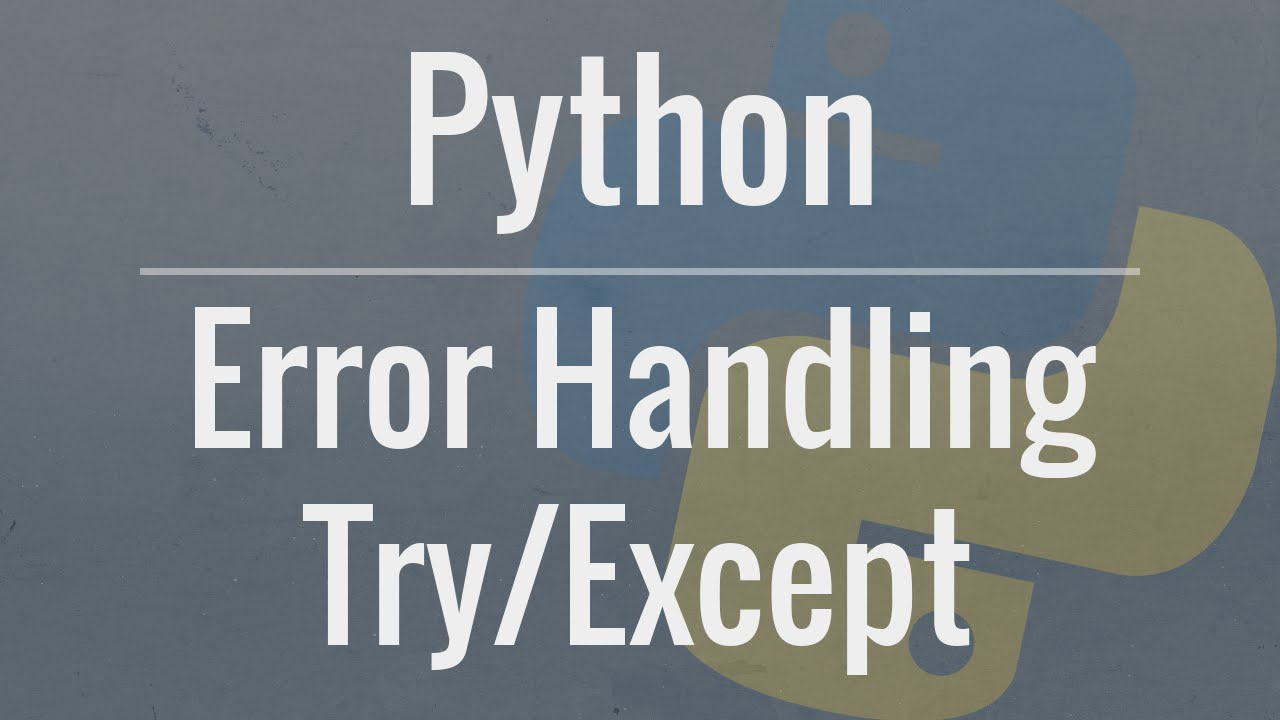
\includegraphics[width=0.60\textwidth]{Gambar/dapi6.jpg}}
 	\caption{Python Exceptions Handling}
 	\label{Python Exceptions Handling}
 \end{figure}
 
 
 
 \section {Pengertian }
 \subsection {Python Exceptions Handling}
 
 
 \hspace*{0.64in} Python menyediakan dua fitur yang sangat penting untuk menangani kesalahan tak terduga dalam program Python Anda dan menambahkan kemampuan debugging di dalamnya Exception Handling: Ini akan dibahas dalam tutorial ini. Berikut adalah daftar standar Pengecualian yang tersedia dengan Python: Pengecualian Standar. Penegasan: Ini akan dibahas dalam Asertions dengan tutorial Python. Daftar Pengecualian Standar – Penegasan dengan Python Penegasan adalah pemeriksaan kewarasan yang dapat Anda aktifkan atau matikan saat Anda selesai dengan pengujian program Anda. Cara termudah untuk memikirkan sebuah pernyataan adalah menyamakannya dengan pernyataan kenaikan gaji-jika (atau lebih akurat, pernyataan kenaikan-jika-tidak). Sebuah ekspresi diuji, dan jika hasilnya muncul salah, pengecualian akan meningkat. Penegasan dilakukan dengan pernyataan tegas, kata kunci terbaru untuk Python, diperkenalkan di versi 1.5. Pemrogram sering menempatkan asersi pada awal fungsi untuk memeriksa masukan yang valid, dan setelah pemanggilan fungsi untuk memeriksa keluaran yang valid. Pernyataan tegas Ketika menemukan pernyataan tegas, Python mengevaluasi ekspresi yang menyertainya, yang semoga benar. Jika ungkapannya salah, Python menimbulkan pengecualian AssertionError. Sintaks untuk menegaskan adalah -menegaskan Ekspresi [, Argumen]. 
 
 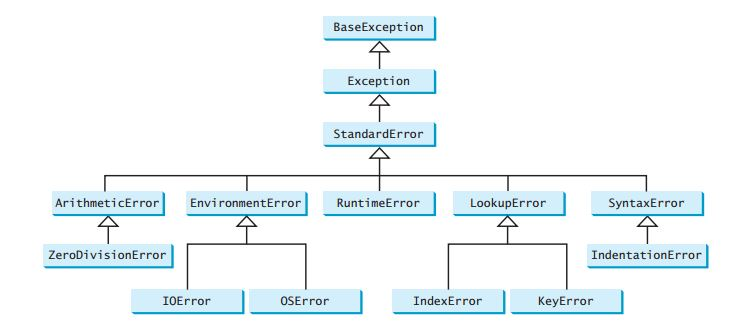
\includegraphics[width=15cm,height=7cm]{Gambar/dapi5.jpg}
 \begin{equation}Python Exceptions Handling\end{equation}
 

\section{Kelas dasar untuk semua pengecualian } 

\subsection{EXCEPTION NAME }

\vspace{12pt}
 \begin{enumerate}
\item StopIteration 

Dibesarkan ketika metode (iterator) berikutnya dari iterator tidak mengarah ke objek apa pun. 
\vspace{12pt}

\item SystemExit 
Dibesarkan oleh fungsi sys.exit () 
\vspace{12pt}

\item StandardError 
 
Kelas dasar untuk semua pengecualian built-in kecuali StopIteration dan SystemExit 
\vspace{12pt}

\item ArithmeticError 
 
Kelas dasar untuk semua kesalahan yang terjadi untuk perhitungan numerik. 
\vspace{12pt}

\item OverflowError 

Dibesarkan saat perhitungan melebihi batas maksimum untuk tipe numerik.
\vspace{12pt}

\item FloatingPointError   

Dibesarkan saat perhitungan floating point gagal. 
\vspace{12pt}

\item ZeroDivisionError  

Dibesarkan saat pembagian atau modulo nol dilakukan untuk semua tipe numerik. 
\vspace{12pt}
\vspace{12pt}

\item AssertionError 

Dibesarkan jika terjadi kegagalan pernyataan Assert. 
\vspace{12pt}

\item AttributeError 
 
Dibesarkan jika terjadi kegagalan referensi atribut atau penugasan.
\vspace{12pt}

\item EOFError 

Dibesarkan bila tidak ada input dari fungsi raw $  \_  $input () atau input () dan akhir file tercapai. 
\vspace{12pt}

\item ImportError 

Dibesarkan saat sebuah pernyataan impor gagal. 
\vspace{12pt}

\item KeyboardInterrupt  

Dibesarkan saat pengguna menyela eksekusi program, biasanya dengan menekan Ctrl + c. 
\vspace{12pt}

\item LookupError  

Kelas dasar untuk semua kesalahan pencarian. 
\vspace{12pt}


\item KeyError 
 
Dibesarkan saat sebuah indeks tidak ditemukan secara berurutan. Dibesarkan saat kunci yang ditentukan tidak ditemukan dalam kamus. 
\vspace{12pt}

\item NameError 

Dibesarkan saat pengenal tidak ditemukan di namespace lokal atau global. 
\vspace{12pt}



\item EnvironmentError  
 
Dibesarkan saat mencoba mengakses variabel lokal dalam suatu fungsi atau metode namun tidak nilai yang ditugaskan padanya. Kelas dasar untuk semua pengecualian yang terjadi di luar lingkungan Python. 
\vspace{12pt}


\item IOError 

IOError Dibesarkan saat operasi input / output gagal, seperti pernyataan cetak atau fungsi open () saat mencoba membuka file yang tidak ada. Dibangkitkan untuk kesalahan terkait sistem operasi. 
\vspace{12pt}

\end {enumerate}
 
\section{SyntaxError} 

\begin{enumerate}


\item IndentationError 

Dibesarkan saat ada kesalahan dengan sintaks Python. Dibesarkan saat indentasi tidak ditentukan dengan benar. 


\item SystemError  

Dibesarkan saat penafsir menemukan masalah internal, namun bila kesalahan ini ditemui juru bahasa Python tidak keluar. 
\vspace{12pt}




\item SystemExit  

Dibesarkan saat juru bahasa Python berhenti dengan menggunakan fungsi sys.exit (). Jika tidak ditangani dalam kode, menyebabkan penafsir untuk keluar. 
\vspace{12pt}


\item TypeError 

Dibesarkan saat operasi atau fungsi dicoba yang tidak valid untuk tipe data yang ditentukan. 
\vspace{12pt}


\item ValueError 

Dibesarkan saat fungsi bawaan untuk tipe data memiliki jenis argumen yang valid, namun argumen tersebut memiliki nilai yang tidak valid yang ditentukan. 
\vspace{12pt}

\item RuntimeError 

Dibesarkan saat kesalahan yang dihasilkan tidak termasuk dalam kategori apa pun. 
\vspace{12pt}

 \end {enumerate}

 \hspace*{0.5in} Jika asersi gagal, Python menggunakan ArgumentExpression sebagai argumen untuk AssertionError. Penegasan Pengecualian pengecualian dapat ditangkap dan ditangani seperti pengecualian lainnya dengan menggunakan perintah try-except, namun jika tidak ditangani, mereka akan menghentikan program dan menghasilkan traceback. 
 
Contoh Berikut adalah fungsi yang mengubah suhu dari derajat Kelvin sampai derajat Fahrenheit. Karena nol derajat Kelvin sedingin yang didapatnya, fungsi itu mundur jika melihat suhu negatif –
\vspace{12pt}
\begin{verbatim}
 $  \#  $!/usr/bin/python 
 
def KelvinToFahrenheit(Temperature): 

~~ assert (Temperature >= 0),"Colder than absolute zero!" 

~~ return ((Temperature-273)*1.8)+32 

print KelvinToFahrenheit(273) 

print int(KelvinToFahrenheit(505.78)) 

print KelvinToFahrenheit(-5) 
\vspace{14pt}

Bila kode diatas dieksekusi, maka menghasilkan hasil sebagai berikut – 
\vspace{12pt}

32.0 

451 

Traceback (most recent call last): 

File "test.py", line 9, in  

print KelvinToFahrenheit(-5) 

File "test.py", line 4, in KelvinToFahrenheit

assert (Temperature >= 0),"Colder than absolute zero!" 

AssertionError: Colder than absolute zero! 
\vspace{12pt}
\end{verbatim}
Apa itu Exception? 

Pengecualian adalah sebuah peristiwa, yang terjadi selama pelaksanaan program yang mengganggu aliran normal instruksi program. Secara umum, ketika skrip Python menemukan situasi yang tidak dapat diatasi, hal itu menimbulkan pengecualian. Pengecualian adalah objek Python yang mewakili kesalahan. 
\vspace{12pt}

Ketika skrip Python menimbulkan pengecualian, ia harus menangani pengecualian begitu saja sehingga berhenti dan berhenti. Menangani pengecualian Jika Anda memiliki beberapa kode yang mencurigakan yang mungkin menimbulkan pengecualian, Anda dapat mempertahankan program Anda dengan menempatkan kode yang mencurigakan di coba: blokir. Setelah dicoba: blokir, sertakan sebuah pernyataan kecuali:, diikuti oleh blok kode yang menangani masalah ini seaman mungkin. Sintaksis Berikut adalah sintaks sederhana coba .... kecuali ... blok lain – 
\vspace{12pt}

\begin{verbatim}
try: 

~~ You do your operations here; 

~~ ...................... 

except \textit{ExceptionI}: 

~~ If there is ExceptionI, then execute this block. 

except \textit{ExceptionII}: 

~~ If there is ExceptionII, then execute this block. 

~~ ...................... 

else: 

~~ If there is no exception then execute this block 
\vspace{12pt}
\vspace{12pt}

\end{verbatim}

Berikut adalah beberapa poin penting tentang sintaks yang disebutkan di atas - 

 \hspace*{0.5in} \vspace{12pt}
\vspace{12pt}

 \hspace*{0.5in} Pernyataan percobaan tunggal dapat memiliki banyak kecuali pernyataan. Ini berguna saat blok coba berisi pernyataan yang mungkin membuang berbagai jenis pengecualian. $  $Anda juga bisa memberikan klausa umum kecuali klausul, yang menangani pengecualian apapun.Setelah klausa kecuali, Anda bisa memasukkan klausul lain. Kode di blok yang lain dijalankan jika kode di coba: blok tidak menimbulkan pengecualian.Blok yang lain adalah tempat yang baik untuk kode yang tidak perlu dicoba: perlindungan blokir. Contoh Contoh ini membuka file, menulis konten di file, dan keluar dengan anggun karena tidak ada masalah sama sekali - 
\vspace{16pt}

\begin{verbatim}

 $  \#  $!/usr/bin/python 
\vspace{12pt}
 
try: 

~~ fh = open("testfile", "w") 

~~ fh.write("This is my test file for exception handling!!") 

except IOError: 

~~ print "Error: can $  \setminus  $'t find file or read data" 

else: 

~~ print "Written content in the file successfully" 

~~ fh.close() 
\vspace{16pt}

Ini menghasilkan hasil sebagai berikut - 
\vspace{12pt}

Written content in the file successfully 
\vspace{12pt}
 
 \end{verbatim}
 
Klausul kecuali tanpa pengecualian anda juga dapat menggunakan pernyataan kecuali tanpa pengecualian yang didefinisikan sebagai berikut - 
\vspace{12pt}

\begin{verbatim}

try: 

~~ You do your operations here; 

~~ ...................... 

except:

~~ If there is any exception, then execute this block. 

~~ ...................... 

else: 

~~ If there is no exception then execute this block.  
\vspace{12pt}
\vspace{16pt}

\end{verbatim}

 \hspace*{0.5in} Pernyataan try-except semacam ini menangkap semua pengecualian yang terjadi. Dengan menggunakan jenis try-except statement ini tidak dianggap sebagai praktik pemrograman yang bagus, karena menangkap semua pengecualian namun tidak membuat programmer mengenali akar permasalahan yang mungkin terjadi. Klausul Kecuali dengan Beberapa Pengecualian Anda juga dapat menggunakan pernyataan kecuali yang sama untuk menangani beberapa pengecualian sebagai berikut - 
\vspace{12pt}
 
try: 

~~ You do your operations here; 

~~ ...................... 

except(Exception1[, Exception2[,...ExceptionN]]]): 

~~ If there is any exception from the given exception list,  

~~ then execute this block. 

~~ ...................... 

else: 

~~ If there is no exception then execute this block.  
\vspace{12pt}
\vspace{12pt}
 
 $  \#  $!/usr/bin/python 
\vspace{12pt}

try: 

~~ fh = open("testfile", "w") 

~~ fh.write("This is my test file for exception handling!!") 
 
finally: 

~~ print "Error: can $  \setminus  $'t find file or read data" 
\vspace{12pt}
\vspace{12pt}
 
 $  \#  $!/usr/bin/python 
\vspace{12pt}
 
try: 

~~ fh = open("testfile", "w") 

~~ try: 
 
~~~~~ fh.write("This is my test file for exception handling!!") 

~~ finally: 

~~~~~ print "Going to close the file" 

~~~~~ fh.close() 

except IOError: 

~~ print "Error: can $  \setminus  $'t find file or read data" 
\vspace{12pt}
\vspace{16pt}

 \hspace*{0.5in} Bila dikecualikan dilempar di blok coba, eksekusi langsung lolos ke blok akhirnya. Setelah semua pernyataan di blok akhirnya dieksekusi, pengecualian dinaikkan lagi dan ditangani dalam pernyataan kecuali jika ada di lapisan yang lebih tinggi dari pernyataan try-except. Argumen Eksepsi Pengecualian dapat memiliki argumen, yang merupakan nilai yang memberi informasi tambahan tentang masalah tersebut. Isi argumen bervariasi menurut pengecualian. Anda menangkap argumen pengecualian dengan menyediakan sebuah variabel dalam klausa kecuali sebagai berikut - 
\vspace{12pt}

try: 

~~ You do your operations here;

~~ ...................... 

except \textit{ExceptionType}\textit{,}\textit{ }\textit{Argument}: 

~~ You can print value of Argument here... 
\vspace{12pt}

 \hspace*{0.5in} Jika Anda menulis kode untuk menangani satu pengecualian, Anda dapat memiliki variabel mengikuti nama pengecualian dalam pernyataan kecuali. Jika Anda menjebak beberapa pengecualian, Anda dapat memiliki variabel mengikuti tuple pengecualian. Variabel ini menerima nilai pengecualian yang sebagian besar mengandung penyebab pengecualian. Variabel tersebut dapat menerima satu nilai atau beberapa nilai dalam bentuk tuple. Tuple ini biasanya berisi error string, error number, dan error location. Pengecualian yang Ditentukan Pengguna Python juga memungkinkan Anda membuat pengecualian sendiri dengan menurunkan kelas dari pengecualian standar built-in. Berikut adalah contoh yang berkaitan dengan RuntimeError. Di sini, sebuah kelas dibuat yang dikelompokkan dari RuntimeError. Ini berguna saat Anda perlu menampilkan informasi yang lebih spesifik saat pengecualian tertangkap. Di blok percobaan, pengecualian yang ditentukan pengguna dinaikkan dan ditangkap di blok kecuali. Variabel e digunakan untuk membuat sebuah instance dari class Networkerror. 
\vspace{12pt}

{\fontsize{10pt}{10pt}\selectfont  (x,y) = (5,0)} 

{\fontsize{10pt}{10pt}\selectfont  try:} 

{\fontsize{10pt}{10pt}\selectfont ~~ z = x/y} 


{\fontsize{10pt}{10pt}\selectfont  except ZeroDivisionError:}


{\fontsize{10pt}{10pt}\selectfont ~~ print "divide by zero"} 

\vspace{10pt}

Jika Anda ingin memeriksa pengecualian dari kode, Anda bisa memiliki: 

\vspace{12pt}
 
\vspace{12pt}

\vspace{12pt}

{\fontsize{10pt}{10pt}\selectfont  (x,y) = (5,0)} 


{\fontsize{10pt}{10pt}\selectfont  try:} 


{\fontsize{10pt}{10pt}\selectfont ~~ z = x/y} 


{\fontsize{10pt}{10pt}\selectfont  except ZeroDivisionError as e:} 

{\fontsize{10pt}{10pt}\selectfont ~~ z = e  $  \#  $ representation: "<exceptions.ZeroDivisionError instance at 0x817426c>"} 


{\fontsize{10pt}{10pt}\selectfont  print z  $  \#  $ output: "integer division or modulo by zero"} 

\vspace{16pt}

General Error Catching 

\vspace{12pt}
 
 \hspace*{0.64in} Terkadang, Anda ingin menangkap semua kesalahan yang mungkin dihasilkan, tapi biasanya Anda tidak melakukannya. Dalam kebanyakan kasus, Anda ingin menjadi sespesifik mungkin (CatchWhatYouCanHandle). Pada contoh pertama di atas, jika Anda menggunakan klausul pengecualian catch-all dan pengguna menekan Ctrl-C, menghasilkan KeyboardInterrupt, Anda tidak ingin program mencetak "bagi dengan nol". Namun, ada beberapa situasi di mana yang terbaik untuk menangkap semua kesalahan. Misalnya, Anda menulis modul ekstensi ke layanan web. Anda ingin informasi kesalahan untuk output output halaman web, dan server untuk terus berjalan, jika mungkin. Tapi Anda tidak tahu kesalahan apa yang mungkin Anda masukkan ke dalam kode Anda. Dalam situasi seperti ini, Anda mungkin ingin mengode sesuatu seperti ini: 
\vspace{12pt}


{\fontsize{10pt}{10pt}\selectfont  import sys}
 

{\fontsize{10pt}{10pt}\selectfont  try:} 


{\fontsize{10pt}{10pt}\selectfont ~~ untrusted.execute()} 


{\fontsize{10pt}{10pt}\selectfont  except:  $  \#  $ catch *all* exceptions} 


{\fontsize{10pt}{10pt}\selectfont ~~ e = sys.exc $  \_  $info()[0]} 


{\fontsize{10pt}{10pt}\selectfont ~~ write $  \_  $to $  \_  $page( "<p>Error:  $  \%  $s</p>"  $  \%  $ e )} 
\vspace{10pt}

 \hspace*{0.64in} Menemukan Nama Pengecualian Spesifik Pengecualian standar yang dapat diajukan dijelaskan secara rinci pada: $  $
 Lihatlah dokumentasi kelas untuk mengetahui pengecualian apa yang bisa diberikan oleh kelas tertentu. Lihat juga: Di wiki ini: WritingExceptionClasses, TracebackModule. Untuk gagasan umum (non-Python specific) tentang pengecualian, berkonsultasilah dengan ExceptionPatterns. Untuk menulis tentang ... 

\vspace{12pt}
 
\begin{itemize}
\item Berikan contoh IOError, dan interpretasikan kode IOError. 

\item Berikan contoh beberapa pengecualian. Penanganan beberapa kecuali dalam satu baris.\end{itemize}
 
 
\vspace{12pt}

Pertanyaan Penanganan Kesalahan Umum, Di bagian "penanganan kesalahan umum" di atas, tertulis untuk menangkap semua pengecualian, Anda menggunakan kode berikut: 
\vspace{14pt}
 
{\fontsize{10pt}{10pt}\selectfont import sys} 


{\fontsize{10pt}{10pt}\selectfont  try:} 

\vspace{10pt}
 

{\fontsize{10pt}{10pt}\selectfont ~~ untrusted.execute()} 

\vspace{10pt}


{\fontsize{10pt}{10pt}\selectfont  except:  $  \#  $ catch *all* exceptions} 

\vspace{10pt}


{\fontsize{10pt}{10pt}\selectfont ~~ e = sys.exc $  \_  $info()[0]} 

\vspace{10pt}


{\fontsize{10pt}{10pt}\selectfont ~~ write $  \_  $to $  \_  $page( "<p>Error:  $  \%  $s</p>"  $  \%  $ e )} 
\vspace{16pt}


{\fontsize{10pt}{10pt}\selectfont  try:}

\vspace{10pt}
 
 
{\fontsize{10pt}{10pt}\selectfont ~~ untrusted.execute()} 

\vspace{10pt}

 
{\fontsize{10pt}{10pt}\selectfont  except Exception as e:} 

\vspace{10pt}

 
{\fontsize{10pt}{10pt}\selectfont ~~ write $  \_  $to $  \_  $page( "<p>Error:  $  \%  $s</p>"  $  \%  $ str(e) )} 
\vspace{16pt}

 \hspace*{0.64in} Seseorang menunjukkan bahwa "kecuali" menangkap lebih dari sekedar "kecuali Pengecualian sebagai e." Mengapa demikian? Apa bedanya? – LionKimbro Untuk saat ini (versi <= 2.4) pengecualian tidak harus diwarisi dari Exception. Jadi polos 'kecuali:'nangkap semua pengecualian, tidak hanya sistem. Pengecualian string adalah salah satu contoh pengecualian yang tidak mewarisi dari Exception. – MikeRovner Saya percaya bahwa pada 2,7, pengecualian masih tidak harus diwariskan dari Exception atau bahkan BaseException. Namun, seperti Python 3, pengecualian harus subclass BaseException. - gajah jim Mendapatkan Informasi Berguna dari Pengecualian Jadi, saya punya sesuatu seperti: 
 
\vspace{12pt}


{\fontsize{10pt}{10pt}\selectfont  (a,b,c) = d} 

\vspace{12pt}
 
dan Python kembali: 
 
\vspace{12pt}
 
 
{\fontsize{10pt}{10pt}\selectfont  ValueError: unpack list of wrong size} 
\vspace{16pt}

... dan begitulah, Anda tentu bertanya-tanya, "Nah, apa yang ada di d?" 

\vspace{12pt}

Anda tahu - Anda bisa mencetak di sana, dan itu berhasil. Tapi adakah cara yang lebih baik dan lebih menarik untuk mendapatkan informasi yang diketahui orang? Anda bisa melakukan sesuatu seperti: 
\vspace{20pt}

 
 try: 
 
 
~~ a, b, c = d 
 
 
 except Exception as e: 
 
 
~~ e.args += (d,) 
 
 
~~ raise 
\vspace{20pt}
 
 \hspace*{0.64in} Atribut .args pengecualian adalah tuple dari semua argumen yang dilewatkan (biasanya argumen satu dan satu-satunya adalah pesan kesalahannya). Dengan cara ini Anda dapat mengubah argumen dan menaikkan kembali, dan informasi tambahan akan ditampilkan. Anda juga bisa membuat pernyataan cetak atau login di blok kecuali. Perhatikan bahwa tidak semua pengecualian subclass Exception (meski hampir semua dilakukan), jadi ini mungkin tidak menangkap beberapa pengecualian; Selain itu, pengecualian tidak diperlukan untuk memiliki atribut .args (meskipun jika pengecualian subclass Exception dan tidak mengesampingkan  $  \_  $ $  \_  $init $  \_  $ $  \_  $ tanpa memanggil superclass-nya), maka kode yang ditulis mungkin gagal Namun dalam prakteknya hampir tidak pernah (dan Jika ya, Anda harus memperbaiki pengecualian yang tidak sesuai!) Bukankah lebih baik mencegahnya untuk melakukan remediasi? >  
 Joel Spolsky mungkin programmer hebat C ++, dan sarannya untuk desain antarmuka pengguna sangat berharga, tapi Python bukan C ++ atau Java, dan argumennya tentang pengecualian tidak berlaku dengan Python. Joel berpendapat: "Mereka tidak terlihat dalam kode sumber Melihat kumpulan kode, termasuk fungsi yang mungkin atau mungkin tidak membuang pengecualian, tidak ada cara untuk melihat pengecualian mana yang mungkin dilempar dan dari mana.Ini berarti bahwa pemeriksaan kode yang hati-hati pun tidak. Saya bisa mengungkapkan potensi bug. " 

 \hspace*{0.64in} (Perhatikan bahwa ini juga merupakan argumen di balik pengecualian yang diperiksa oleh Java - sekarang eksplisit bahwa pengecualian dapat dilemparkan - kecuali bahwa RuntimeException masih dapat dibuang ke mana saja. -jJ) Saya tidak mengerti argumen ini. Dalam kode sumber acak, tidak ada cara untuk mengetahui apakah akan gagal hanya dengan inspeksi. Jika Anda melihat: 

\vspace{12pt}

\vspace{12pt}

x = 1 

result = myfunction (x) 
\vspace{20pt}

 \hspace*{0.64in} Anda tidak dapat mengetahui apakah fungsi saya gagal pada saat runtime hanya dengan inspeksi, jadi mengapa harus itu penting apakah gagal menabrak pada saat runtime atau gagal dengan meningkatkan pengecualian? 
 
\vspace{12pt}
 
(Crashing itu buruk Dengan secara eksplisit menyatakan pengecualian, Anda memperingatkan orang-orang bahwa mereka mungkin ingin mengatasinya Jawa melakukannya dengan canggung C tidak memiliki cara yang baik untuk melakukannya sama sekali, karena kesalahan kembali masih di band Untuk pengembalian reguler Di python, pengecualian passthrough tidak ditandai, namun kondisi kesalahan menonjol di tempat mereka diciptakan, dan biasanya tidak meniru hasil yang benar. -jJ)

 \hspace*{0.64in} Argumen Joel yang mengemukakan pengecualian hanyalah sebuah goto yang menyamar sebagian benar. Tapi begitu juga untuk loop, sementara loop, fungsi dan metode! Seperti konstruksi lainnya, pengecualian adalah gotos yang dijinakkan dan dipekerjakan untuk Anda, bukan yang liar dan berbahaya. Anda tidak bisa melompat * di mana saja *, hanya tempat yang sangat terbatas. 
 
\vspace{12pt}

Joel juga menulis: 

\vspace{12pt}
 
 \hspace*{0.64in} "Mereka membuat terlalu banyak titik keluar yang mungkin untuk sebuah fungsi.Untuk menulis kode yang benar, Anda benar-benar harus memikirkan setiap jalur kode yang mungkin melalui fungsi Anda. Setiap kali Anda memanggil fungsi yang dapat meningkatkan pengecualian dan tidak menangkapnya di Spot, Anda menciptakan peluang untuk kejutan bug yang disebabkan oleh fungsi yang dihentikan tiba-tiba, meninggalkan data dalam keadaan tidak konsisten, atau jalur kode lainnya yang tidak Anda pikirkan. " 
 
\vspace{12pt}
 
\vspace{10pt}
\vspace{12pt}

try: 
 
~~ You do your operations here; 

~~ ...................... 
 
except(Exception1[, Exception2[,...ExceptionN]]]): 
 
~~ If there is any exception from the given exception list,  

~~ then execute this block. 

~~ ...................... 

else: 
 
~~ If there is no exception then execute this block.  
\vspace{12pt}
\vspace{12pt}
 
 $  \#  $!/usr/bin/python 
\vspace{12pt}

try: 
 
~~ fh = open("testfile", "w") 

~~ fh.write("This is my test file for exception handling!!") 

finally: 

~~ print "Error: can $  \setminus  $'t find file or read data" 
\vspace{12pt}
\vspace{12pt}
 
 $  \#  $!/usr/bin/python 
\vspace{12pt}
 
try: 
 
~~ fh = open("testfile", "w") 

~~ try: 
 
~~~~~ fh.write("This is my test file for exception handling!!") 

~~ finally: 
 
~~~~~ print "Going to close the file" 

~~~~~ fh.close() 

except IOError: 
 
~~ print "Error: can $  \setminus  $'t find file or read data" 
\vspace{12pt}
\vspace{12pt}
\vspace{12pt}
\vspace{12pt}
Bila dikecualikan dilempar di blok coba, eksekusi langsung lolos ke blok akhirnya. Setelah semua pernyataan di blok akhirnya dieksekusi, pengecualian dinaikkan lagi dan ditangani dalam pernyataan kecuali jika ada di lapisan yang lebih tinggi dari pernyataan try-except. Argumen Eksepsi. Python juga memungkinkan Anda membuat pengecualian sendiri dengan menurunkan kelas dari pengecualian standar built-in. Berikut adalah contoh yang berkaitan dengan RuntimeError. Di sini, sebuah kelas dibuat yang dikelompokkan dari RuntimeError. Ini berguna saat Anda perlu menampilkan informasi yang lebih spesifik saat pengecualian tertangkap. Di blok percobaan, pengecualian yang ditentukan pengguna dinaikkan dan ditangkap di blok kecuali. Variabel e digunakan untuk membuat sebuah instance dari class Networkerror. 
\vspace{18pt}


\subsection{Python Regular Exceptions}
 Exceptions reguler adalah urutan khusus karakter yang membantu Anda mencocokkan atau menemukan string atau rangkaian senar lainnya, menggunakan sintaks khusus yang dipegang dalam sebuah pola. Ekspresi reguler banyak digunakan di dunia UNIX. Modul ini memberikan dukungan penuh untuk ekspresi reguler seperti Perl dengan Python. Modul re meningkatkan pengecualian re.error jika terjadi kesalahan saat mengkompilasi atau menggunakan ekspresi reguler.Kami akan membahas dua fungsi penting, yang akan digunakan untuk menangani ekspresi reguler. Tapi ada hal kecil dulu: Ada berbagai karakter, yang tentunya memiliki arti khusus bila digunakan dalam ekspresi reguler. Untuk menghindari kebingungan saat berhadapan dengan ekspresi reguler, kita akan menggunakan Raw Strings sebagai r'expression '.
\subsubsection{Fungsi Pertandingan}
Fungsi ini mencoba mencocokkan pola RE dengan string dengan flag pilihan.
Berikut adalah sintaks untuk fungsi ini :
\begin{enumerate}
\item Parameter, Ini adalah ekspresi reguler yang harus disesuaikan.
\item String, Ini adalah string, yang akan dicari agar sesuai dengan pola pada awal string.
\item flags, Anda dapat menentukan flag yang berbeda menggunakan bitwise OR ( \$ \$). Ini adalah pengubah, yang tercantum dalam tabel di bawah ini. fungsi mengembalikan objek yang cocok pada kesuksesan, None on failure. Kami mengelompokkan (num) atau kelompok () fungsi objek pencocokan untuk mendapatkan ekspresi yang sesuai.
\end{enumerate}

\subsection{Match Object Methods}
\begin{enumerate}
\item Metode ini mengembalikan seluruh kecocokan (atau jumlah subkelompok tertentu.
\item Metode ini mengembalikan semua subkelompok yang cocok dalam tupel (kosong jika tidak ada)
\end{enumerate}

\begin{verbatim}


 $  \#  $! / Usr / bin / python
Impor kembali

Line = "Kucing lebih pintar dari pada anjing"

MatchObj = re.match (r '(. *) Adalah (. *?). *', Line, re.M  $    $ re.I)

jika cocokObj:

~~ cetak "matchObj.group ():", matchObj.group ()

~~ cetak "matchObj.group (1):", matchObj.group (1)

~~ Cetak "matchObj.group (2):", matchObj.group (2)

lain:

~~ cetak "Tidak ada pertandingan !!"
\end{verbatim}

Bila kode diatas dieksekusi, maka menghasilkan hasil sebagai berikut -

MatchObj.group (): Kucing lebih pintar dari pada anjing

MatchObj.group (1): Kucing

MatchObj.group (2): lebih pintar

Fungsi Pencarian

Fungsi ini mencari kejadian pertama dari pola RE dalam string dengan flag pilihan.

Berikut adalah sintaks untuk fungsi ini:

Re.search (pola, string, flag = 0)

Berikut adalah deskripsi parameternya:
Parameter pattern Ini adalah ekspresi reguler yang harus disesuaikan. String Ini adalah string, yang akan dicari agar sesuai dengan pola di manapun dalam string. Flags Anda dapat menentukan flag yang berbeda menggunakan bitwise OR ( \$    \$). Ini adalah pengubah, yang tercantum dalam tabel di bawah ini.Fungsi re.search mengembalikan objek yang cocok pada kesuksesan, tidak ada yang gagal. Kami menggunakan fungsi kelompok (num) atau kelompok () dari objek pertandingan untuk mendapatkan ekspresi yang sesuai.Match Object Methods Descriptiongroup(num=0) Metode ini mengembalikan seluruh kecocokan (atau jumlah subkelompok tertentu)groups()Metode ini mengembalikan semua subkelompok yang cocok dalam tupel (kosong jika tidak ada)

\begin{verbatim}
 $  \#  $!/usr/bin/python

import re

line = "Cats are smarter than dogs";

searchObj = re.search( r'(.*) are (.*?) .*', line, re.M $    $re.I)

if searchObj:

~~ print "searchObj.group() : ", searchObj.group()

~~ print "searchObj.group(1) : ", searchObj.group(1)

~~ print "searchObj.group(2) : ", searchObj.group(2)

else:
~~ print "Nothing found!!"

searchObj.group()~:  Cats are smarter than dogs

searchObj.group(1)~:  Cats

searchObj.group(2)~:  smarter
\end{verbatim}

\subsection{Pencocokan Versus Searching}
Python menawarkan dua operasi primitif yang berbeda berdasarkan ekspresi reguler: cek kecocokan untuk kecocokan hanya di awal string, sementara pencarian memeriksa kecocokan di manapun dalam string (inilah yang Perl lakukan secara default).
Contoh:

\begin{verbatim}


 $  \#  $!/usr/bin/python

import re

line = "Cats are smarter than dogs";

matchObj = re.match( r'dogs', line, re.M $   $re.I)

if matchObj:

~~ print "match --> matchObj.group() : ", matchObj.group()

else:

~~ print "No match!!"

searchObj = re.search( r'dogs', line, re.M $    $re.I)

if searchObj:

~~ print "search --> searchObj.group() : ", searchObj.group()

else:

~~ print "Nothing found!!"

No match!!

search~--> matchObj.group() :  dogs
\end{verbatim}


\subsection{Cari dan Ganti}
Salah satu metode re yang paling penting yang menggunakan ekspresi reguler adalah sub.

  \subsubsection{Sintaksis}
  Re.sub (pola, repl, string, max = 0)

  Metode ini menggantikan semua kemunculan pola RE dalam string dengan repl, mengganti semua kejadian kecuali jika max diberikan. Metode ini mengembalikan string yang dimodifikasi.
  Contoh
  \begin{verbatim}
   $  \#  $!/usr/bin/python

  import re

  phone = "2004-959-559  $  #  $ This is Phone Number"

  $  #  $ Delete Python-style comments

  num = re.sub(r' $  #  $.* $  $  $', "", phone)
  print "Phone Num : ", num
  $  #  $ Remove anything other than digits
  num~=~re.sub(r' $  $D',~"", phone)
  print "Phone Num : ", num
  Phone~Num :  2004-959-559
  Phone~Num :  2004959559
  \end{verbatim}
\subsection{Regular Expression Modifiers: Option Flags}
Ekspresi reguler literal mungkin termasuk pengubah opsional untuk mengendalikan berbagai aspek pencocokan. Pengubah ditentukan sebagai bendera pilihan. Anda dapat memberikan beberapa pengubah menggunakan OR eksklusif ( \$   \$), seperti yang ditunjukkan sebelumnya dan dapat ditunjukkan oleh salah satu dari ini – Modifier Description
re.I
Lakukan pencocokan case-insensitive.
re.L
Menafsirkan kata-kata sesuai dengan lokal saat ini. Interpretasi ini mempengaruhi kelompok abjad ( \verb|$   $ w dan  $   $| W), serta perilaku batas kata ( \verb|$    $ b dan  $    $| B).
re.M
Membuat  \$  \$  \$ cocok dengan akhir baris (bukan hanya akhir string) dan membuat  \$   \$ cocok dengan awal baris apapun (bukan hanya permulaan string).
re.S
Membuat sebuah periode (dot) cocok dengan karakter apapun, termasuk newline.
re.U
Menginterpretasikan huruf sesuai dengan karakter Unicode. Flag ini mempengaruhi perilaku  \verb|$    $ w,  $    $ W,  $    $ b,  $   $ |B.
re.X
Memungkinkan sintaks ekspresi reguler "manis". Ini mengabaikan spasi (kecuali di dalam himpunan [] atau saat diloloskan oleh garis miring terbalik) dan memperlakukan unescaped  \$  \#  \$ sebagai tanda komentar.
\subsection{Pola Ekspresi Reguler}
Kecuali karakter kontrol, (+?.  \verb|$   $  $   $  $  \$  $ () []  $  \{  $ $  \}  $  $    $  $  $|), Semua karakter cocok dengan karakter mereka sendiri. Anda bisa lolos dari karakter kontrol sebelum mendahului dengan garis miring terbalik.
Berikut daftar tabel sintaks ekspresi reguler yang tersedia dengan Python -
\begin{verbatim}
 $  \#  $!/usr/bin/python
import re
phone = "2004-959-559  $  #  $ This is Phone Number"
 $  \#  $ Delete Python-style comments
num = re.sub(r' $  \#  $.* $  \$  $', "", phone)
print "Phone Num : ", num
 $  \#  $ Remove anything other than digits
num~=~re.sub(r' $    $D',~"", phone)
print "Phone Num : ", num
Phone~Num :  2004-959-559
Phone~Num :  2004959559
<Directory "/var/www/cgi-bin">
~~ AllowOverride None
~~ Options ExecCGI
~~ Order allow,deny
~~ Allow from all
</Directory>
<Directory "/var/www/cgi-bin">
Options All
</Directory>
!/usr/bin/python
print "Content-type:text/html $  \setminus  $r $  \setminus  $n $  \setminus  $r $  \setminus  $n"
print '<html>'
print '<head>'
print '<title>Hello Word - First CGI Program</title>'
print '</head>'
print '<body>'
print '<h2>Hello Word! This is my first CGI program</h2>'
print '</body>'
print '</html>'
\end{verbatim}
Halo kata! Ini adalah program CGI pertamaku
Script hello.py ini adalah skrip Python yang sederhana, yang menuliskan hasilnya pada file STDOUT, yaitu layar. Ada satu fitur penting dan tambahan yang tersedia yang merupakan baris pertama yang akan dicetak Content-type: text / html  \verb|$    $ r  $    $ n  $    $ r  $    $| n. Baris ini dikirim kembali ke browser dan ini menentukan jenis konten yang akan ditampilkan di layar browser. Sekarang Anda pasti sudah mengerti konsep dasar CGI dan Anda bisa menulis banyak program CGI yang rumit dengan menggunakan Python. Script ini bisa berinteraksi dengan sistem eksternal lainnya juga untuk bertukar informasi seperti RDBMS.
\subsection{Header HTTP}
nt-type: text / html  \verb|$    $ r  $    $ n  $    $ r  $    $| n adalah bagian dari header HTTP yang dikirim ke browser untuk memahami isinya. Semua header HTTP akan berada dalam bentuk berikut -
\begin{verbatim}
 $  \#  $!/usr/bin/python
 $  \#  $ Import modules for CGI handling
import cgi, cgitb
 $  \#  $ Create instance of FieldStorage
form = cgi.FieldStorage()
 $  \#  $ Get data from fields
first $  \_  $name = form.getvalue('first $  \_  $name')
last $  \_  $name~ = form.getvalue('last $  \_  $name')
print "Content-type:text/html $  \setminus  $r $  \setminus  $n $  \setminus  $r $  \setminus  $n"
print "<html>"
print "<head>"
print "<title>Hello - Second CGI Program</title>"
print "</head>"
print "<body>"
print "<h2>Hello  $  \%  $s  $  \%  $s</h2>"  $  \%  $ (first $  \_  $name, last $  \_  $name)
print "</body>"
print "</html>"
<form action="/cgi-bin/hello $  \_  $get.py" method="get">
First~Name: <input type="text" name="first $  \_  $name">  <br />
Last Name: <input type="text" name="last $  \_  $name" />
<input type="submit" value="Submit" />
</form>
 $  \#  $!/usr/bin/python
 $  \#  $ Import modules for CGI handling
import cgi, cgitb
 $  \#  $ Create instance of FieldStorage
form = cgi.FieldStorage()
$  \#  $ Get data from fields
first $  \_  $name = form.getvalue('first $  \_  $name')
last $  \_  $name~ = form.getvalue('last $  \_  $name')
print "Content-type:text/html $  \setminus  $r $  \setminus  $n $  \setminus  $r $  \setminus  $n"
print "<html>"
print "<head>"
print "<title>Hello - Second CGI Program</title>"
print "</head>"
print "<body>"
print "<h2>Hello  $  \%  $s  $  \%  $s</h2>"  $  \%  $ (first $  \_  $name, last $  \_  $name)
print "<body>"
print "</html>"
<form action="/cgi-bin/hello $  \_  $get.py" method="post">
First~Name: <input type="text" name="first $  \_  $name"> <br />
Last Name: <input type="text" name="last $  \_  $name"/>
<input type="submit" value="Submit" />
</form>
\end{verbatim}
Mari kita ambil lagi contoh yang sama seperti di atas yang melewati dua nilai menggunakan HTML FORMULIR dan tombol kirim. Kami menggunakan skrip CGI yang sama hello $  \_  $get.py untuk menangani masukan ini.
Melewati Data Kotak Centang ke Program CGI
Kotak centang digunakan bila lebih dari satu pilihan diperlukan untuk dipilih.
Berikut adalah contoh kode HTML untuk form dengan dua kotak centang -
Melewati Data Tombol Radio ke Program CGI
Tombol Radio digunakan bila hanya satu pilihan yang harus dipilih.
Berikut adalah contoh kode HTML untuk form dengan dua tombol radio
\begin{verbatim}
$  \#  $!/usr/bin/python
 $  \#  $ Import modules for CGI handling
import cgi, cgitb
 $  \#  $ Create instance of FieldStorage
form = cgi.FieldStorage()
$  \#  $ Get data from fields
if form.getvalue('subject'):
~~ subject = form.getvalue('subject')
else:
~~ subject = "Not set"
print "Content-type:text/html $  \setminus  $r $  \setminus  $n $  \setminus  $r $  \setminus  $n"
print "<html>"
print "<head>"
print "<title>Radio - Fourth CGI Program</title>"
print "</head>"
print "<body>"
print "<h2> Selected Subject is  $  \%  $  $  \%  $s</h2>"  $  \%  $ subject
print "</body>"
print "</html>"
<form action="/cgi-bin/textarea.py" method="post" target=" $  \_  $blank">
<textarea name="textcontent" cols="40" rows="4">
Type your text here...
</textarea>
<input type="submit" value="Submit" />
</form>
 $  \#  $!/usr/bin/python
 $  \#  $ Import modules for CGI handling
import cgi, cgitb
 $  \#  $ Create instance of FieldStorage
form = cgi.FieldStorage()
 $  \#  $ Get data from fields
if form.getvalue('textcontent'):
~~ text $  \_  $content = form.getvalue('textcontent')
else:
~~ text $  \_  $content = "Not entered"
print "Content-type:text/html $  \setminus  $r $  \setminus  $n $  \setminus  $r $  \setminus  $n"
print "<html>"
print "<head>"
print "<title>Text Area - Fifth CGI Program</title>"
print "</head>"
print "<body>"
print "<h2> Entered Text Content is  $  \%  $s</h2>"  $  \%  $ text $  \_  $content
print "</body>"
\end{verbatim}
{\fontsize{14pt}{14pt}\selectfont \textbf{Menggunakan Cookies di CGI} \\}
Protokol HTTP adalah protokol tanpa kewarganegaraan. Untuk situs komersial, diperlukan informasi sesi di antara halaman yang berbeda. Misalnya, satu pendaftaran pengguna berakhir setelah menyelesaikan banyak halaman. Bagaimana cara mempertahankan informasi sesi pengguna di semua halaman web? Dalam banyak situasi, menggunakan cookies adalah metode yang paling efisien untuk mengingat dan melacak preferensi, pembelian, komisi, dan informasi lainnya yang diperlukan untuk pengalaman pengunjung atau statistik situs yang lebih baik.
Contoh dasar
Joke: apa yang kamu sebut babi dengan tiga mata? Piiig!
Aturan dasar pencarian ekspresi reguler untuk sebuah pola dalam sebuah string adalah:
Hasil pencarian melalui string dari awal sampai akhir, berhenti pada pertandingan pertama yang ditemukan  Semua pola harus dicocokkan, tapi tidak semua senar Jika cocok = re.search (tepuk, str) berhasil, kecocokan tidak ada dan khususnya match.group () adalah teks yang cocok
\verb|~  $  \#  $ $  \#  $ Search for pattern 'iii' in string 'piiig'|.
\verb|~  $  \#  $ $  \#  $| All of the pattern must match, but it may appear anywhere.
\verb|~  $  \#  $ $  \#  $| On success, match.group() is matched text.
\verb|~~match = re.search(r'iii', 'piiig') =>  found, match.group() == "iii"|
\verb|~~match = re.search(r'igs', 'piiig') =>  not found, match == None|
\verb|~  $  \#  $ $  \#  $ . = any char but  $  \setminus  $n|
\verb|~~match = re.search(r'..g', 'piiig') =>  found, match.group() == "iig"|
\verb|~  $  \#  $ $  \#  $  $  \setminus  $d = digit char,  $  \setminus  $w = word char|
\verb|~~match = re.search(r' $  \setminus  $d $  \setminus  $d $  \setminus  $d', 'p123g') =>  found, match.group() == "123"|
\verb|~~match = re.search(r' $  \setminus  $w $  \setminus  $w $  \setminus  $w', '@@abcd!!') =>  found, match.group() == "abc"|
Pengulangan
Hal menjadi lebih menarik saat Anda menggunakan + dan * untuk menentukan pengulangan dalam polanya
~~~ + - 1 atau lebih kemunculan pola ke kiri, mis. 'I +' = satu atau lebih i's
~~~ * - 0 atau lebih kemunculan pola ke kiri
~~~ ? - cocokkan 0 atau 1 kemunculan pola ke kiri
{\fontsize{14pt}{14pt}\selectfont \textbf{Paling kiri  $  \&  $ terbesar} \\}
Pertama, pencarian menemukan kecocokan paling kiri untuk pola tersebut, dan kedua mencoba menggunakan sebanyak mungkin string - yaitu + dan * sejauh mungkin (huruf + dan * dikatakan "serakah").
Contoh pengulangan
 $  \#  $ $  \#  $ i+ = one or more i's, as many as possible.
\verb|~~match = re.search(r'pi+', 'piiig') =>  found, match.group() == "piii"|
\verb|~  $  \#  $ $  \#  $ Finds the first/leftmost solution, and within it drives the +|
\verb|~  $  \#  $ $  \#  $ as far as possible| (aka 'leftmost and largest').
\verb|~  $  \#  $ $  \#  $| In this example, note that it does not get to the second set of i's.
\verb|~~match = re.search(r'i+', 'piigiiii') =>  found, match.group() == "ii"|
\verb|~  $  \#  $ $  \#  $  $  \setminus  $s* = zero or more whitespace chars|
\verb|~  $  \#  $ $  \#  $| Here look for 3 digits, possibly separated by whitespace.
~~match~=~re.search(r' $  \setminus  $d $  \setminus  $s* $  \setminus  $d $  \setminus  $s* $  \setminus  $d',~'xx1~2   3xx') =>  found, match.group() == "1 2   3"
~~match~=~re.search(r' $  \setminus  $d $  \setminus  $s* $  \setminus  $d $  \setminus  $s* $  \setminus  $d', 'xx12  3xx') =>  found, match.group() == "12  3"
~~match = re.search(r' $  \setminus  $d $  \setminus  $s* $  \setminus  $d $  \setminus  $s* $  \setminus  $d', 'xx123xx') =>  found, match.group() == "123"
\verb|~  $  \#  $ $  \#  $  $  \string^  $ = matches the start of string, so this fails:|
\verb|~~match = re.search(r' $  \string^  $b $  \setminus  $w+', 'foobar') =>  not found, match == None|
\verb|~  $  \#  $ $  \#  $ but without the  $  \string^  $ it succeeds:|
~~match = re.search(r'b $  \setminus  $w+', 'foobar') =>  found, match.group() == "bar"
{\fontsize{14pt}{14pt}\selectfont \textbf{Contoh email} \\} \par
Misalkan Anda ingin mencari alamat email di dalam string 'xyz alice-b@google.com ungu monyet'. Kami akan menggunakan ini sebagai contoh yang berjalan untuk menunjukkan fitur ekspresi reguler. Berikut adalah upaya menggunakan pola r ' $  \setminus  $ w + @  $  \setminus  $ w +':
~ Str = 'ungu alice-b@google.com monyet pencuci piring'
~ Match = re.search (r ' $  \setminus  $ w + @  $  \setminus  $ w +', str)
~ Jika cocok:
\verb|~~~ print match.group ()  $  \#  $ $  \#  $ 'b @ google'|
Pencarian tidak mendapatkan keseluruhan alamat email dalam kasus ini karena  $  \setminus  $ w tidak cocok dengan '-' atau '.' Di alamat Kami akan memperbaikinya menggunakan fitur ekspresi reguler di bawah ini. Kurung persegi Tanda kurung siku dapat digunakan untuk menunjukkan sekumpulan karakter, jadi [abc] cocok dengan 'a' atau 'b' atau 'c'. Kode  $  \setminus  $ w,  $  \setminus  $ s dll bekerja di dalam kurung siku juga dengan satu pengecualian bahwa titik (.) Hanya berarti titik literal. Untuk masalah email, tanda kurung siku adalah cara mudah untuk menambahkan '.' Dan '-' ke kumpulan karakter yang dapat muncul di sekitar @ dengan pola r '[ $  \setminus  $ w .-] + @ [ $  \setminus  $ w .-] +' untuk mendapatkan keseluruhan alamat email:
~ Match = re.search (r '[ $  \setminus  $ w .-] + @ [ $  \setminus  $ w .-] +', str)
~ Jika cocok:
~~~ print match.group ()  $  \#  $ $  \#  $ 'alice-b@google.com'
(Lebih banyak fitur kotak-braket) Anda juga dapat menggunakan tanda hubung untuk menunjukkan jangkauan, jadi [a-z] cocok dengan semua huruf kecil. Untuk menggunakan tanda hubung tanpa menunjukkan jangkauan, pasang tanda hubung terakhir, mis. [abc-]. Top-up ( $  \string^  $) pada awal set persegi-braket telah membalikkannya, jadi [ $  \string^  $ ab] berarti karakter apapun kecuali 'a' atau 'b'.
{\fontsize{14pt}{14pt}\selectfont \textbf{Ekstraksi Grup} \\}
Fitur "kelompok" dari ekspresi reguler memungkinkan Anda untuk memilih bagian dari teks yang sesuai. Misalkan untuk masalah email yang ingin kita ekstrak username dan host secara terpisah. Untuk melakukan ini, tambahkan kurung () di sekitar nama pengguna dan host dalam pola, seperti ini: r '([ $  \setminus  $ w .-] +) @ ([ $  \setminus  $ w .-] +)'. Dalam kasus ini, tanda kurung tidak mengubah pola yang akan cocok, sebaliknya mereka membentuk "kelompok" logis dalam teks pertandingan. Pada pencarian yang sukses, match.group (1) adalah teks kecocokan yang sesuai dengan tanda kurung kiri ke 1, dan match.group (2) adalah teks yang sesuai dengan kurung kiri ke-2. Match.group polos () masih merupakan keseluruhan teks pertandingan seperti biasa.
~ Str = 'ungu alice-b@google.com monyet pencuci piring'
\verb|~ Match = re.search ('([ $  \setminus  $ w .-] +) @ ([ $  \setminus  $ w .-] +)', str)|
~ Jika cocok:
\verb|~~~ Print match.group ()  $  \#  $ $  \#  $ 'alice-b@google.com'| (keseluruhan pertandingan)
\verb|~~~ Print match.group (1)  $  \#  $ $  \#  $ 'alice-b'| (nama pengguna, grup 1)
\verb|~~~ Print match.group (2)  $  \#  $ $  \#  $ 'google.com'| (host, grup 2)
Alur kerja umum dengan ekspresi reguler adalah Anda menulis sebuah pola untuk hal yang Anda cari, menambahkan kelompok tanda kurung untuk mengekstrak bagian yang Anda inginkan. Temukan semua Findall () mungkin adalah fungsi tunggal yang paling kuat dalam modul re. Di atas kami menggunakan re.search () untuk menemukan kecocokan pertama untuk sebuah pola. Findall () menemukan * semua * kecocokan dan mengembalikannya sebagai daftar string, dengan masing-masing string mewakili satu kecocokan.
\verb|~  $  \#  $ $  \#  $| Misalkan kita memiliki teks dengan banyak alamat email
~ Str = 'ungu alice@google.com, bla monyet bob@abc.com blah pencuci piring'
\verb|~  $  \#  $ $  \#  $ disini re.findall ()| mengembalikan daftar semua string email yang ditemukan
\verb|~ Email = re.findall (r '[ $  \setminus  $ w  $  \setminus  $ .-] + @ [ $  \setminus  $ w  $  \setminus  $ .-] +', str)  $  \#  $ $  \#  $ ['alice@google.com', 'bob@abc.com']|
~ Untuk email di email:
\begin{verbatim}
~~~  $  \#  $ Lakukan sesuatu dengan setiap string email yang ditemukan
=======
~~ print "Nothing found!!"
searchObj.group()~:  Cats are smarter than dogs
searchObj.group(1)~:  Cats
searchObj.group(2)~:  smarter
\end{verbatim}
\subsection{Pencocokan Versus Searching}
Python menawarkan dua operasi primitif yang berbeda berdasarkan ekspresi reguler: cek kecocokan untuk kecocokan hanya di awal string, sementara pencarian memeriksa kecocokan di manapun dalam string (inilah yang Perl lakukan secara default).
Contoh:
\begin{verbatim}
 $  \#  $!/usr/bin/python
import re
line = "Cats are smarter than dogs";
matchObj = re.match( r'dogs', line, re.M $   $re.I)
if matchObj:
~~ print "match --> matchObj.group() : ", matchObj.group()
else:
~~ print "No match!!"
searchObj = re.search( r'dogs', line, re.M $    $re.I)
if searchObj:
~~ print "search --> searchObj.group() : ", searchObj.group()
else:
~~ print "Nothing found!!"
No match!!
search~--> matchObj.group() :  dogs
\end{verbatim}
\subsection{Cari dan Ganti}
Salah satu metode re yang paling penting yang menggunakan ekspresi reguler adalah sub.
  \subsubsection{Sintaksis}
  Re.sub (pola, repl, string, max = 0)
  Metode ini menggantikan semua kemunculan pola RE dalam string dengan repl, mengganti semua kejadian kecuali jika max diberikan. Metode ini mengembalikan string yang dimodifikasi.
  Contoh
  \begin{verbatim}
   $  \#  $!/usr/bin/python
  import re
  phone = "2004-959-559  $  #  $ This is Phone Number"
  $  #  $ Delete Python-style comments
  num = re.sub(r' $  #  $.* $  $  $', "", phone)

  print "Phone Num : ", num

  $  #  $ Remove anything other than digits

  num~=~re.sub(r' $  $D',~"", phone)

  print "Phone Num : ", num

  Phone~Num :  2004-959-559

  Phone~Num :  2004959559
  \end{verbatim}

\subsection{Regular Expression Modifiers: Option Flags}
Ekspresi reguler literal mungkin termasuk pengubah opsional untuk mengendalikan berbagai aspek pencocokan. Pengubah ditentukan sebagai bendera pilihan. Anda dapat memberikan beberapa pengubah menggunakan OR eksklusif ( \$   \$), seperti yang ditunjukkan sebelumnya dan dapat ditunjukkan oleh salah satu dari ini – Modifier Description
re.I
Lakukan pencocokan case-insensitive.

re.L
Menafsirkan kata-kata sesuai dengan lokal saat ini. Interpretasi ini mempengaruhi kelompok abjad ( \verb|$   $ w dan  $   $| W), serta perilaku batas kata ( \verb|$    $ b dan  $    $| B).

re.M
Membuat  \$  \$  \$ cocok dengan akhir baris (bukan hanya akhir string) dan membuat  \$   \$ cocok dengan awal baris apapun (bukan hanya permulaan string).

re.S
Membuat sebuah periode (dot) cocok dengan karakter apapun, termasuk newline.

re.U
Menginterpretasikan huruf sesuai dengan karakter Unicode. Flag ini mempengaruhi perilaku  \verb|$    $ w,  $    $ W,  $    $ b,  $   $ |B.

re.X
Memungkinkan sintaks ekspresi reguler "manis". Ini mengabaikan spasi (kecuali di dalam himpunan [] atau saat diloloskan oleh garis miring terbalik) dan memperlakukan unescaped  \$  \#  \$ sebagai tanda komentar.

\subsection{Pola Ekspresi Reguler}
Kecuali karakter kontrol, (+?.  \verb|$   $  $   $  $  \$  $ () []  $  \{  $ $  \}  $  $    $  $  $|), Semua karakter cocok dengan karakter mereka sendiri. Anda bisa lolos dari karakter kontrol sebelum mendahului dengan garis miring terbalik.

Berikut daftar tabel sintaks ekspresi reguler yang tersedia dengan Python -
\begin{verbatim}
 $  \#  $!/usr/bin/python

import re

phone = "2004-959-559  $  #  $ This is Phone Number"

 $  \#  $ Delete Python-style comments
num = re.sub(r' $  \#  $.* $  \$  $', "", phone)

print "Phone Num : ", num

 $  \#  $ Remove anything other than digits

num~=~re.sub(r' $    $D',~"", phone)

print "Phone Num : ", num

Phone~Num :  2004-959-559
Phone~Num :  2004959559

<Directory "/var/www/cgi-bin">

~~ AllowOverride None

~~ Options ExecCGI

~~ Order allow,deny

~~ Allow from all

</Directory>

<Directory "/var/www/cgi-bin">

Options All

</Directory>

!/usr/bin/python

print "Content-type:text/html $  \setminus  $r $  \setminus  $n $  \setminus  $r $  \setminus  $n"

print '<html>'

print '<head>'

print '<title>Hello Word - First CGI Program</title>'

print '</head>'

print '<body>'

print '<h2>Hello Word! This is my first CGI program</h2>'

print '</body>'

print '</html>'
\end{verbatim}

Halo kata! Ini adalah program CGI pertamaku

Script hello.py ini adalah skrip Python yang sederhana, yang menuliskan hasilnya pada file STDOUT, yaitu layar. Ada satu fitur penting dan tambahan yang tersedia yang merupakan baris pertama yang akan dicetak Content-type: text / html  \verb|$    $ r  $    $ n  $    $ r  $    $| n. Baris ini dikirim kembali ke browser dan ini menentukan jenis konten yang akan ditampilkan di layar browser. Sekarang Anda pasti sudah mengerti konsep dasar CGI dan Anda bisa menulis banyak program CGI yang rumit dengan menggunakan Python. Script ini bisa berinteraksi dengan sistem eksternal lainnya juga untuk bertukar informasi seperti RDBMS.

\subsection{Header HTTP}
nt-type: text / html  \verb|$    $ r  $    $ n  $    $ r  $    $| n adalah bagian dari header HTTP yang dikirim ke browser untuk memahami isinya. Semua header HTTP akan berada dalam bentuk berikut -

\begin{verbatim}

 $  \#  $!/usr/bin/python

 $  \#  $ Import modules for CGI handling

import cgi, cgitb

 $  \#  $ Create instance of FieldStorage

form = cgi.FieldStorage()

 $  \#  $ Get data from fields

first $  \_  $name = form.getvalue('first $  \_  $name')

last $  \_  $name~ = form.getvalue('last $  \_  $name')

print "Content-type:text/html $  \setminus  $r $  \setminus  $n $  \setminus  $r $  \setminus  $n"

print "<html>"

print "<head>"

print "<title>Hello - Second CGI Program</title>"

print "</head>"

print "<body>"

print "<h2>Hello  $  \%  $s  $  \%  $s</h2>"  $  \%  $ (first $  \_  $name, last $  \_  $name)

print "</body>"

print "</html>"

<form action="/cgi-bin/hello $  \_  $get.py" method="get">

First~Name: <input type="text" name="first $  \_  $name">  <br />

Last Name: <input type="text" name="last $  \_  $name" />

<input type="submit" value="Submit" />

</form>

 $  \#  $!/usr/bin/python

 $  \#  $ Import modules for CGI handling

import cgi, cgitb

 $  \#  $ Create instance of FieldStorage

form = cgi.FieldStorage()

$  \#  $ Get data from fields

first $  \_  $name = form.getvalue('first $  \_  $name')

last $  \_  $name~ = form.getvalue('last $  \_  $name')

print "Content-type:text/html $  \setminus  $r $  \setminus  $n $  \setminus  $r $  \setminus  $n"

print "<html>"

print "<head>"

print "<title>Hello - Second CGI Program</title>"

print "</head>"

print "<body>"

print "<h2>Hello  $  \%  $s  $  \%  $s</h2>"  $  \%  $ (first $  \_  $name, last $  \_  $name)

print "<body>"

print "</html>"

<form action="/cgi-bin/hello $  \_  $get.py" method="post">

First~Name: <input type="text" name="first $  \_  $name"> <br />

Last Name: <input type="text" name="last $  \_  $name"/>

<input type="submit" value="Submit" />

</form>

\end{verbatim}
Mari kita ambil lagi contoh yang sama seperti di atas yang melewati dua nilai menggunakan HTML FORMULIR dan tombol kirim. Kami menggunakan skrip CGI yang sama hello $  \_  $get.py untuk menangani masukan ini.

Melewati Data Kotak Centang ke Program CGI

Kotak centang digunakan bila lebih dari satu pilihan diperlukan untuk dipilih.

Berikut adalah contoh kode HTML untuk form dengan dua kotak centang -

Melewati Data Tombol Radio ke Program CGI

Tombol Radio digunakan bila hanya satu pilihan yang harus dipilih.

Berikut adalah contoh kode HTML untuk form dengan dua tombol radio
\begin{verbatim}
$  \#  $!/usr/bin/python

 $  \#  $ Import modules for CGI handling

import cgi, cgitb

 $  \#  $ Create instance of FieldStorage

form = cgi.FieldStorage()

$  \#  $ Get data from fields

if form.getvalue('subject'):

~~ subject = form.getvalue('subject')

else:

~~ subject = "Not set"

print "Content-type:text/html $  \setminus  $r $  \setminus  $n $  \setminus  $r $  \setminus  $n"

print "<html>"

print "<head>"

print "<title>Radio - Fourth CGI Program</title>"

print "</head>"

print "<body>"

print "<h2> Selected Subject is  $  \%  $  $  \%  $s</h2>"  $  \%  $ subject

print "</body>"

print "</html>"

<form action="/cgi-bin/textarea.py" method="post" target=" $  \_  $blank">

<textarea name="textcontent" cols="40" rows="4">

Type your text here...

</textarea>

<input type="submit" value="Submit" />

</form>

 $  \#  $!/usr/bin/python

 $  \#  $ Import modules for CGI handling

import cgi, cgitb

 $  \#  $ Create instance of FieldStorage

form = cgi.FieldStorage()

 $  \#  $ Get data from fields

if form.getvalue('textcontent'):

~~ text $  \_  $content = form.getvalue('textcontent')

else:

~~ text $  \_  $content = "Not entered"

print "Content-type:text/html $  \setminus  $r $  \setminus  $n $  \setminus  $r $  \setminus  $n"

print "<html>"

print "<head>"

print "<title>Text Area - Fifth CGI Program</title>"

print "</head>"

print "<body>"

print "<h2> Entered Text Content is  $  \%  $s</h2>"  $  \%  $ text $  \_  $content

print "</body>"

\end{verbatim}

{\fontsize{14pt}{14pt}\selectfont \textbf{Menggunakan Cookies di CGI} \\}

Protokol HTTP adalah protokol tanpa kewarganegaraan. Untuk situs komersial, diperlukan informasi sesi di antara halaman yang berbeda. Misalnya, satu pendaftaran pengguna berakhir setelah menyelesaikan banyak halaman. Bagaimana cara mempertahankan informasi sesi pengguna di semua halaman web? Dalam banyak situasi, menggunakan cookies adalah metode yang paling efisien untuk mengingat dan melacak preferensi, pembelian, komisi, dan informasi lainnya yang diperlukan untuk pengalaman pengunjung atau statistik situs yang lebih baik.

Contoh dasar

Joke: apa yang kamu sebut babi dengan tiga mata? Piiig!

Aturan dasar pencarian ekspresi reguler untuk sebuah pola dalam sebuah string adalah:

Hasil pencarian melalui string dari awal sampai akhir, berhenti pada pertandingan pertama yang ditemukan  Semua pola harus dicocokkan, tapi tidak semua senar Jika cocok = re.search (tepuk, str) berhasil, kecocokan tidak ada dan khususnya match.group () adalah teks yang cocok

\verb|~  $  \#  $ $  \#  $ Search for pattern 'iii' in string 'piiig'|.

\verb|~  $  \#  $ $  \#  $| All of the pattern must match, but it may appear anywhere.

\verb|~  $  \#  $ $  \#  $| On success, match.group() is matched text.

\verb|~~match = re.search(r'iii', 'piiig') =>  found, match.group() == "iii"|

\verb|~~match = re.search(r'igs', 'piiig') =>  not found, match == None|

\verb|~  $  \#  $ $  \#  $ . = any char but  $  \setminus  $n|

\verb|~~match = re.search(r'..g', 'piiig') =>  found, match.group() == "iig"|

\verb|~  $  \#  $ $  \#  $  $  \setminus  $d = digit char,  $  \setminus  $w = word char|

\verb|~~match = re.search(r' $  \setminus  $d $  \setminus  $d $  \setminus  $d', 'p123g') =>  found, match.group() == "123"|

\verb|~~match = re.search(r' $  \setminus  $w $  \setminus  $w $  \setminus  $w', '@@abcd!!') =>  found, match.group() == "abc"|

Pengulangan

Hal menjadi lebih menarik saat Anda menggunakan + dan * untuk menentukan pengulangan dalam polanya

~~~ + - 1 atau lebih kemunculan pola ke kiri, mis. 'I +' = satu atau lebih i's

~~~ * - 0 atau lebih kemunculan pola ke kiri

~~~ ? - cocokkan 0 atau 1 kemunculan pola ke kiri

{\fontsize{14pt}{14pt}\selectfont \textbf{Paling kiri  $  \&  $ terbesar} \\}
Pertama, pencarian menemukan kecocokan paling kiri untuk pola tersebut, dan kedua mencoba menggunakan sebanyak mungkin string - yaitu + dan * sejauh mungkin (huruf + dan * dikatakan "serakah").

Contoh pengulangan

 $  \#  $ $  \#  $ i+ = one or more i's, as many as possible.

\verb|~~match = re.search(r'pi+', 'piiig') =>  found, match.group() == "piii"|

\verb|~  $  \#  $ $  \#  $ Finds the first/leftmost solution, and within it drives the +|

\verb|~  $  \#  $ $  \#  $ as far as possible| (aka 'leftmost and largest').

\verb|~  $  \#  $ $  \#  $| In this example, note that it does not get to the second set of i's.

\verb|~~match = re.search(r'i+', 'piigiiii') =>  found, match.group() == "ii"|

\verb|~  $  \#  $ $  \#  $  $  \setminus  $s* = zero or more whitespace chars|

\verb|~  $  \#  $ $  \#  $| Here look for 3 digits, possibly separated by whitespace.

~~match~=~re.search(r' $  \setminus  $d $  \setminus  $s* $  \setminus  $d $  \setminus  $s* $  \setminus  $d',~'xx1~2   3xx') =>  found, match.group() == "1 2   3"

~~match~=~re.search(r' $  \setminus  $d $  \setminus  $s* $  \setminus  $d $  \setminus  $s* $  \setminus  $d', 'xx12  3xx') =>  found, match.group() == "12  3"

~~match = re.search(r' $  \setminus  $d $  \setminus  $s* $  \setminus  $d $  \setminus  $s* $  \setminus  $d', 'xx123xx') =>  found, match.group() == "123"

\verb|~  $  \#  $ $  \#  $  $  \string^  $ = matches the start of string, so this fails:|

\verb|~~match = re.search(r' $  \string^  $b $  \setminus  $w+', 'foobar') =>  not found, match == None|

\verb|~  $  \#  $ $  \#  $ but without the  $  \string^  $ it succeeds:|

~~match = re.search(r'b $  \setminus  $w+', 'foobar') =>  found, match.group() == "bar"

{\fontsize{14pt}{14pt}\selectfont \textbf{Contoh email} \\} \par
Misalkan Anda ingin mencari alamat email di dalam string 'xyz alice-b@google.com ungu monyet'. Kami akan menggunakan ini sebagai contoh yang berjalan untuk menunjukkan fitur ekspresi reguler. Berikut adalah upaya menggunakan pola r ' $  \setminus  $ w + @  $  \setminus  $ w +':

~ Str = 'ungu alice-b@google.com monyet pencuci piring'

~ Match = re.search (r ' $  \setminus  $ w + @  $  \setminus  $ w +', str)

~ Jika cocok:

\verb|~~~ print match.group ()  $  \#  $ $  \#  $ 'b @ google'|

Pencarian tidak mendapatkan keseluruhan alamat email dalam kasus ini karena  $  \setminus  $ w tidak cocok dengan '-' atau '.' Di alamat Kami akan memperbaikinya menggunakan fitur ekspresi reguler di bawah ini. Kurung persegi Tanda kurung siku dapat digunakan untuk menunjukkan sekumpulan karakter, jadi [abc] cocok dengan 'a' atau 'b' atau 'c'. Kode  $  \setminus  $ w,  $  \setminus  $ s dll bekerja di dalam kurung siku juga dengan satu pengecualian bahwa titik (.) Hanya berarti titik literal. Untuk masalah email, tanda kurung siku adalah cara mudah untuk menambahkan '.' Dan '-' ke kumpulan karakter yang dapat muncul di sekitar @ dengan pola r '[ $  \setminus  $ w .-] + @ [ $  \setminus  $ w .-] +' untuk mendapatkan keseluruhan alamat email:

~ Match = re.search (r '[ $  \setminus  $ w .-] + @ [ $  \setminus  $ w .-] +', str)

~ Jika cocok:

~~~ print match.group ()  $  \#  $ $  \#  $ 'alice-b@google.com'

(Lebih banyak fitur kotak-braket) Anda juga dapat menggunakan tanda hubung untuk menunjukkan jangkauan, jadi [a-z] cocok dengan semua huruf kecil. Untuk menggunakan tanda hubung tanpa menunjukkan jangkauan, pasang tanda hubung terakhir, mis. [abc-]. Top-up ( $  \string^  $) pada awal set persegi-braket telah membalikkannya, jadi [ $  \string^  $ ab] berarti karakter apapun kecuali 'a' atau 'b'.

{\fontsize{14pt}{14pt}\selectfont \textbf{Ekstraksi Grup} \\}
Fitur "kelompok" dari ekspresi reguler memungkinkan Anda untuk memilih bagian dari teks yang sesuai. Misalkan untuk masalah email yang ingin kita ekstrak username dan host secara terpisah. Untuk melakukan ini, tambahkan kurung () di sekitar nama pengguna dan host dalam pola, seperti ini: r '([ $  \setminus  $ w .-] +) @ ([ $  \setminus  $ w .-] +)'. Dalam kasus ini, tanda kurung tidak mengubah pola yang akan cocok, sebaliknya mereka membentuk "kelompok" logis dalam teks pertandingan. Pada pencarian yang sukses, match.group (1) adalah teks kecocokan yang sesuai dengan tanda kurung kiri ke 1, dan match.group (2) adalah teks yang sesuai dengan kurung kiri ke-2. Match.group polos () masih merupakan keseluruhan teks pertandingan seperti biasa.

~ Str = 'ungu alice-b@google.com monyet pencuci piring'

\verb|~ Match = re.search ('([ $  \setminus  $ w .-] +) @ ([ $  \setminus  $ w .-] +)', str)|

~ Jika cocok:

\verb|~~~ Print match.group ()  $  \#  $ $  \#  $ 'alice-b@google.com'| (keseluruhan pertandingan)

\verb|~~~ Print match.group (1)  $  \#  $ $  \#  $ 'alice-b'| (nama pengguna, grup 1)

\verb|~~~ Print match.group (2)  $  \#  $ $  \#  $ 'google.com'| (host, grup 2)

Alur kerja umum dengan ekspresi reguler adalah Anda menulis sebuah pola untuk hal yang Anda cari, menambahkan kelompok tanda kurung untuk mengekstrak bagian yang Anda inginkan. Temukan semua Findall () mungkin adalah fungsi tunggal yang paling kuat dalam modul re. Di atas kami menggunakan re.search () untuk menemukan kecocokan pertama untuk sebuah pola. Findall () menemukan * semua * kecocokan dan mengembalikannya sebagai daftar string, dengan masing-masing string mewakili satu kecocokan.

\verb|~  $  \#  $ $  \#  $| Misalkan kita memiliki teks dengan banyak alamat email

~ Str = 'ungu alice@google.com, bla monyet bob@abc.com blah pencuci piring'

\verb|~  $  \#  $ $  \#  $ disini re.findall ()| mengembalikan daftar semua string email yang ditemukan

\verb|~ Email = re.findall (r '[ $  \setminus  $ w  $  \setminus  $ .-] + @ [ $  \setminus  $ w  $  \setminus  $ .-] +', str)  $  \#  $ $  \#  $ ['alice@google.com', 'bob@abc.com']|

~ Untuk email di email:

~~~  $  \#  $ Lakukan sesuatu dengan setiap string email yang ditemukan

~~~ Cetak email


\chapter{Clasess/Object}
\section{Pengertian }
\subsection{Python Object Oriented}
Phyton merupakan bahasa pemrograman yang berorientasi obyek dinamis, dapat digunakan untuk bermacam-macam pengembangan perangkat lunak. Phyton menyediakan dukungan yang kuat untuk integrasi dengan bahasa pemrograman lain dan alat-alat bantu lainnya.
Object Oriented Programming (OOP) adalah sebuah pendekatan pemrograman dimana objek didefinisikan dengan metode (fungsi, action, atau events) dan sifat (nilai serta karakteristik), sehingga mudah dibaca, lebih banyak kode yang dapat digunakan kembali.
Python telah menjadi bahasa berorientasi objek sejak itu ada. Karena itu, menciptakan dan menggunakan kelas dan objek sangat mudah. Bab ini membantu Anda menjadi ahli dalam menggunakan dukungan pemrograman berorientasi objek
Objek adalah sesuatu yang menamping nilai atau data dan dapat dikenakan operasi tertentu:
\begin {enumerate}
\item Class atau Kelas: adalah struktur data yang bisa digunakan untuk mendefinisikan objek yang menyimpan data bersama-sama nilai-nilai dan perilaku. Kelas adalah suatu entitas yang merupakan bentuk program dari suatu abstraksi untuk permasalahan dunia nyata, dan instans dari class merupakan realisasi dari beberapa objek.
\item Inheritace atau pewarisan merupakan konsep dalam pemrograman berbasis objek yang memungkinkan untuk membuat suatu kelas dengan didasarkan pada kelas yang sudah ada sehingga mewarisi semua method dan atributnya. Dengan cara seperti ini, semua method dan atribut yang terdapat pada kelas induk diturunkan ke kelas turunannya. Namun kelas turunannya dapat menambah method baru atau atribut baru tersendiri.
\item Method Constructor merupakan sebuah method yang akan otomatis dipanggil ketika objek diinstantiasi. Construktor umumnya digunakan untuk melakukan inisialisasi terhadap suatu variabel atau method.
\end {enumerate}
Jika Anda tidak memiliki pengalaman sebelumnya dengan pemrograman berorientasi objek (OO), Anda mungkin  ingin berkonsultasi dengan kursus perkenalan atau setidaknya tutorial semacam itu sehingga Anda dapat memahami konsep dasarnya. Namun, di sini adalah pengenalan kecil Object-Oriented Programming (OOP) untuk membawa Anda pada kecepatan - Ikhtisar Terminologi OOP.

\begin{enumerate}
\item Kelas: Prototipe yang ditentukan pengguna untuk objek yang mendefinisikan seperangkat atribut yang menjadi ciri objek kelas apa pun. Atribut adalah data anggota (variabel kelas dan variabel contoh) dan metode, diakses melalui notasi titik.
\item Variabel kelas: Variabel yang dimiliki oleh semua instance kelas. Variabel kelas didefinisikan dalam kelas tapi di luar metode kelas manapun. Variabel kelas tidak digunakan sesering variabel contoh.
\item Anggota data: Variabel kelas atau variabel contoh yang menyimpan data yang terkait dengan kelas dan objeknya.
\item Fungsi overloading: Penugasan lebih dari satu perilaku ke fungsi tertentu. Operasi yang dilakukan bervariasi menurut jenis objek atau argumen yang terlibat.
\item Contoh variabel: Variabel yang didefinisikan di dalam metode dan hanya dimiliki oleh instance kelas saat ini.
\item Warisan: Pengalihan karakteristik kelas ke kelas lain yang berasal darinya. Contoh: Objek individual dari kelas tertentu. Obyek obj yang termasuk dalam Lingkaran kelas, misalnya, adalah turunan dari Lingkaran kelas.
\item Instansiasi: Pembuatan sebuah instance dari sebuah kelas.

\item Metode: Jenis fungsi khusus yang didefinisikan dalam definisi kelas.  
\item Objek: Contoh unik dari struktur data yang didefinisikan oleh kelasnya. Objek terdiri dari kedua anggota data (variabel kelas dan variabel contoh) dan metode.
\item Operator overloading: Penugasan lebih dari satu fungsi ke operator tertentu.
\end{enumerate}

Salah satu alasan yang paling penting untuk mempertimbangkan bekerja di OOP adalah bahwa ia menyediakan pendekatan pemodelan langsung dan memecahkan masalah didunia nyata.


\subsection{Membuat Kelas}

Pernyataan kelas membuat definisi kelas baru. Nama kelas segera mengikuti kelas kata kunci diikuti oleh titik dua sebagai berikut -

class ClassName:
~~ 'Optional class documentation string'
~~ class $  \_  $suite


Kelas memiliki kumpulan dokumentasi, yang bisa diakses melalui ClassName . $  \_  $ $  \_  $ doc $  \_  $ $  \_  $.  Class $  \_  $suite terdiri dari semua pernyataan komponen yang mendefinisikan anggota kelas, atribut dan fungsi data.

Berikut adalah contoh kelas Python sederhana -
\begin{verbatim}
class Employee:
~~ 'Common base class for all employees'
~~ empCount = 0

~~ def  $  \_  $ $  \_  $init $  \_  $ $  \_  $(self, name, salary):
~~~~~ self.name = name ~~~~~ self.salary = salary
~~~~~ Employee.empCount += 1
~~~~~ def displayCount(self):
~~~~~ print "Total Employee  $  \%  $d"  $  \%  $ Employee.empCount
~~ def displayEmployee(self):

~~~~~~print "Name : ", self.name,  ", Salary: ", self.salary
\end{verbatim}

\subsection{Variable empCount}

Variabel empCount adalah variabel kelas yang nilainya dibagi di antara semua contoh kelas ini. Ini bisa diakses sebagai Employee.empCount dari dalam kelas atau di luar kelas. Metode pertama  $  \_  $ $  \_  $init  $  \_  $ $  \_ $ () adalah metode khusus, yang disebut metode konstruktor kelas atau inisialisasi yang Python panggil saat Anda membuat instance baru dari kelas ini. Anda menyatakan metode kelas lain seperti fungsi normal dengan pengecualian bahwa argumen pertama untuk setiap metode adalah self. Python menambahkan argumen diri ke daftar untuk Anda; Anda tidak perlu memasukkannya saat Anda memanggil metode.

\subsection{Membuat Instance Objects}
Untuk membuat contoh kelas, Anda memanggil kelas menggunakan nama kelas dan meneruskan argumen apa pun yang diterima metode  $  \_  $ $  \_  $init $  \_  $ $  \_  $-nya.

"Ini akan menciptakan objek pertama kelas Karyawan"
Emp1 = Karyawan ("Zara", 2000)
"Ini akan menciptakan objek kedua dari kelas Karyawan"
Emp2 = Karyawan ("Manni", 5000)


\subsection{Mengakses Atribut}
Anda mengakses atribut objek menggunakan dot operator dengan objek. Variabel kelas akan diakses dengan menggunakan nama kelas sebagai berikut -

Emp1.displayEmployee ()
Emp2.displayEmployee (
Cetak "Jumlah Karyawan $  \%  $ d" $  \%  $ Employee.empCount

Sekarang, meletakkan semua konsep bersama -
\begin{verbatim}
 $  \#  $!/usr/bin/python
class Employee:
~~ 'Common base class for all employees'
~~ empCount = 0
~~ def  $  \_  $ $  \_  $init $  \_  $ $  \_  $(self, name, salary):
~~~~~ self.name = name
~~~~~ self.salary = salary
~~~~~ Employee.empCount += 1
~~ def displayCount(self):
~~~~ print "Total Employee  $  \%  $d"  $  \%  $ Employee.empCount
~~ def displayEmployee(self):
~~~~~~print "Name : ", self.name,  ", Salary: ", self.salary
"This would create first object of Employee class"
emp1 = Employee("Zara", 2000)
"This would create second object of Employee class"
emp2 = Employee("Manni", 5000)
emp1.displayEmployee()
emp2.displayEmployee()
print "Total Employee  $  \%  $d"  $  \%  $ Employee.empCount
\end{verbatim}
When the above code is executed, it produces the following result  \$ - \$

Name~:~ Zara ,Salary:  2000
Name~:~ Manni ,Salary:  5000
Total Employee 2
You can add, remove, or modify attributes of classes and objects at any time  \$ - \$
emp1.age~= 7  \ $  \#  $ Add an 'age' attribute.
emp1.age~= 8   \$  \#  $ Modify 'age' attribute.
del~emp1.age  \$  \#  $ Delete 'age' attribute.

Alih-alih menggunakan pernyataan normal untuk mengakses atribut, Anda dapat menggunakan fungsi berikut -

~~~ Getattr (obj, name [, default]): untuk mengakses atribut objek.

~~~ Hasattr (obj, name): untuk memeriksa apakah ada atribut atau tidak.


~~~ Setattr (obj, name, value): untuk mengatur atribut. Jika atribut tidak ada, maka akan dibuat.


~~~ The delattr (obj, name): untuk menghapus sebuah atribut.


Hasattr (emp1, 'age')  \$  \#  \$ Mengembalikan true jika atribut 'age' ada

Getattr (emp1, 'age')  \$  \#  \$ Mengembalikan nilai atribut 'age'

Setattr (emp1, 'age', 8)  \$  \#  \$ Set attribute 'age' di 8
\noindent
Delattr (empl, 'age')  \$  \#  \$ Hapus atribut 'umur'


Atribut Atribut Built-In

Setiap kelas Python terus mengikuti atribut bawaan dan mereka dapat diakses menggunakan operator dot seperti atribut lainnya -

\verb|~~~  $  \_  $ $  \_  $dict $  \_  $ $  \_  $|: Kamus yang berisi namespace kelas.

\verb|~~~  $  \_  $ $  \_  $doc $  \_  $ $  \_  $|: String dokumentasi kelas atau tidak, jika tidak terdefinisi.
\verb| ~~~  $  \_  $ $  \_  $name $  \_  $ $  \_  $|: nama kelas
\verb|~~~  $  \_  $ $  \_  $module $  \_  $ $  \_  $|: Nama modul dimana kelas didefinisikan. Atribut ini " $  \_  $ $  \_  $main $  \_  $ $  \_  $" dalam mode interaktif.
\verb|~~~  $  \_  $ $  \_  $bases $  \_  $ $  \_  $|: Tupel yang mungkin kosong yang berisi kelas dasar, sesuai urutan kejadiannya dalam daftar kelas dasar.

Untuk kelas di atas mari kita coba untuk mengakses semua atribut ini –
\begin{verbatim}
 $  \#  $!/usr/bin/python
class Employee:
~~ 'Common base class for all employees'
~~ empCount = 0
~~ def  $  \_  $ $  \_  $init $  \_  $ $  \_  $(self, name, salary):
~~~~~ self.name = name
~~~~~ self.salary = salary
~~~~~ Employee.empCount += 1
~~ def displayCount(self):
~~~~ print "Total Employee  $  \%  $d"  $  \%  $ Employee.empCount
~~ def displayEmployee(self): \par
~~~~~~print "Name : ", self.name,  ", Salary: ", self.salary
print "Employee. $  \_  $ $  \_  $doc $  \_  $ $  \_  $:", Employee. $  \_  $ $  \_  $doc $  \_  $ $  \_  $
print "Employee. $  \_  $ $  \_  $name $  \_  $ $  \_  $:", Employee. $  \_  $ $  \_  $name $  \_  $ $  \_  $
print "Employee. $  \_  $ $  \_  $module $  \_  $ $  \_  $:", Employee. $  \_  $ $  \_  $module $  \_  $ $  \_  $
print "Employee. $  \_  $ $  \_  $bases $  \_  $ $  \_  $:", Employee. $  \_  $ $  \_  $bases $  \_  $ $  \_  $
print "Employee. $  \_  $ $  \_  $dict $  \_  $ $  \_  $:", Employee. $  \_  $ $  \_  $dict $  \_  $ $  \_  $
\end{verbatim}

Bila kode diatas dieksekusi, maka menghasilkan hasil sebagai berikut -
Karyawan . \verb|$  \_  $ $  \_  $ doc $  \_  $ $  \_  $|: kelas dasar umum untuk semua karyawan
Karyawan . \verb|$  \_  $ $  \_  $ name $  \_  $ $  \_  $|: Karyawan
Karyawan . \verb|$  \_  $ $  \_  $ modul $  \_  $ $  \_  $|:  $  \_  $ $  \_  $main $  \_  $ $  \_  $
Karyawan . \verb|$  \_  $ $  \_  $ bases $  \_  $ $  \_  $|: ()
Karyawan . \verb|$  \_  $ $  \_  $ dict $  \_  $ $  \_  $|:  $  \{  $' $  \_  $ $  \_  $module $  \_  $ $  \_  $': ' $  \_  $ $  \_  $main $  \_  $ $  \_  $', 'displayCount':
<function displayCount at 0xb7c84994>, 'empCount': 2,
'DisplayEmployee': <function displayEmployee at 0xb7c8441c>,
\verb|' $  \_  $ $  \_  $doc $  \_  $ $  \_  $|': 'Kelas dasar umum untuk semua karyawan',
\verb|' $  \_  $ $  \_  $init $  \_  $ $  \_  $|': <function  $  \_  $ $  \_  $init $  \_  $ $  \_  $ di 0xb7c846bc> $  \}  $ \par

\subsection{Menghancurkan Objek (Pengumpulan Sampah)}
Python menghapus objek yang tidak dibutuhkan (tipe built-in atau instance kelas) secara otomatis untuk membebaskan ruang memori. Proses dimana Python secara berkala mengumpulkan kembali blok memori yang tidak lagi digunakan disebut Koleksi Sampah. Pengumpul sampah Python berjalan selama eksekusi program dan dipicu saat penghitungan referensi objek mencapai nol. Jumlah referensi referensi berubah karena jumlah alias yang menunjukkannya berubah. Jumlah referensi objek meningkat saat diberi nama baru atau ditempatkan dalam wadah (daftar, tupel, atau kamus). Jumlah referensi objek berkurang saat dihapus dengan del, rujukannya ditugaskan kembali, atau rujukannya tidak sesuai. Ketika penghitungan referensi objek mencapai nol, Python mengumpulkannya secara otomatis.
a = 40  \$  \#  \$ Buat objek <40>
B = a  \$  \#  \$ Tingkatkan ref. Hitung <40>
c = [b]  \$  \#  \$ Tingkatkan ref. Hitung <40>
Del  $  \#  $ Penurunan ref. Hitung <40>
b = 100  $  \#  $ Kurangi ref. Hitung <40>
C [0] = -1  $  \#  $ Kurangi ref. Hitung <40>


Anda biasanya tidak akan memperhatikan kapan pengumpul sampah menghancurkan contoh yatim piatu dan mengembalikan ruangnya. Tapi kelas bisa menerapkan metode khusus  $  \_  $ $  \_  $del  $  \_  $ $  \_ $ (), yang disebut destructor, yang dipanggil saat instance tersebut hendak dimusnahkan. Metode ini bisa digunakan untuk membersihkan sumber daya non memori yang digunakan oleh sebuah instance. \par

Contoh
Penghancur  \verb|$  \_  $ $  \_  $del  $  \_  $ $  \_  $| () ini mencetak nama kelas sebuah instance yang akan dihancurkan -
\begin{verbatim}
$  \#  $!/usr/bin/python
class Point:
~~ def  $  \_  $ $  \_  $init $  \_  $ $  \_  $( self, x=0, y=0):
~~~~~ self.x = x
~~~~~ self.y = y
~~ def  $  \_  $ $  \_  $del $  \_  $ $  \_  $(self):
~~~~~ class $  \_  $name = self. $  \_  $ $  \_  $class $  \_  $ $  \_  $. $  \_  $ $  \_  $name $  \_  $ $  \_  $
~~~~~ print class $  \_  $name, "destroyed"
pt1 = Point()
pt2 = pt1
pt3 = pt1
print id(pt1), id(pt2), id(pt3)  $  \#  $ prints the ids of the obejcts
del pt1
del pt2
del pt3
\end{verbatim}

\subsection{Kelas Warisan}
Alih-alih mulai dari nol, Anda dapat membuat kelas dengan menurunkannya dari kelas yang sudah ada sebelumnya dengan mencantumkan kelas induk dalam tanda kurung setelah nama kelas yang baru. Kelas anak mewarisi atribut kelas induknya, dan Anda dapat menggunakan atribut tersebut seolah-olah mereka didefinisikan di kelas anak. Kelas anak juga dapat mengesampingkan data anggota dan metode dari orang tua. Sintaksis Kelas turunan dinyatakan seperti kelas orang tua mereka; Namun, daftar kelas dasa yang diwarisi dari diberikan setelah nama kelas -

Kelas SubClassName (ParentClass1 [, ParentClass2, ...]):
\begin{verbatim}
~~ 'String dokumentasi kelas opsional'
~~ Class $  \_  $suite
 $  \#  $!/usr/bin/python

class~Parent:~~~~~~   $  \#  $ define parent class
~~ parentAttr = 100
~~ def  $  \_  $ $  \_  $init $  \_  $ $  \_  $(self):
~~~~~ print "Calling parent constructor"
~~ def parentMethod(self):
~~~~~ print 'Calling parent method'
~~ def setAttr(self, attr):
~~~~~ Parent.parentAttr = attr
~~ def getAttr(self):
~~~~~ print "Parent attribute :", Parent.parentAttr
class Child(Parent):  $  \#  $ define child class
~~ def  $  \_  $ $  \_  $init $  \_  $ $  \_  $(self):
~~~~~ print "Calling child constructor"
~~ def childMethod(self):
~~~~~ print 'Calling child method'
c~=~Child()~~~~~~~    $  \#  $ instance of child
c.childMethod()~~~~~  $  \#  $ child calls its method
c.parentMethod()~~~~  $  \#  $ calls parent's method
c.setAttr(200)~~~~~~  $  \#  $ again call parent's method
c.getAttr()~~~~~~~~~  $  \#  $ again call parent's method
Calling child constructor
Calling child method
Calling parent method
Parent attribute : 200
class~A:~~~~~~   $  \#  $ define your class A
.....
class~B:~~~~~~~   $  \#  $ define your class B
.....
class~C(A,~B):    $  \#  $ subclass of A and B
\end{verbatim}

Anda dapat menggunakan fungsi issubclass () atau isinstance () untuk memeriksa hubungan dua kelas dan contoh. Fungsi boolean issubclass (sub, sup) mengembalikan true jika sub subclass yang diberikan memang merupakan subclass dari superclass sup. The isinstance (obj, Class) fungsi boolean mengembalikan true jika obj adalah turunan dari Class Class atau merupakan instance dari subclass of Class.

\subsection{Metode utama}
Anda selalu dapat mengganti metode kelas induk Anda. Salah satu alasan untuk mengesampingkan metode orang tua adalah karena Anda mungkin menginginkan fungsi khusus atau berbeda di subkelas Anda. \par
Contoh
\begin{verbatim}
 $  \#  $! / Usr / bin / python
class parent:  $  \#  $ define parent class
~~ Def myMethod (diri):
~~~~~ Cetak 'metode induk panggilan'

Kelas anak (orang tua):  $  \#  $ define child class
~~ Def myMethod (diri):
~~~~~ Cetak 'metode memanggil anak'
C = Anak ()  $  \#  $ contoh anak
C.myMethod ()  $  \#  $ metode panggilan balik anak
\end{verbatim}
Bila kode diatas dieksekusi, maka menghasilkan hasil sebagai berikut -
Memanggil metode anak
Metode Base Overloading
Berikut daftar tabel beberapa fungsionalitas generik yang dapat Anda timpa di kelas Anda sendiri -

\subsection{Operator overloading}
Misalkan Anda telah membuat kelas Vektor untuk mewakili vektor dua dimensi, apa yang terjadi bila Anda menggunakan operator plus untuk menambahkannya? Kemungkinan besar Python akan berteriak pada Anda. Anda bisa, bagaimanapun, menentukan metode  $  \_  $ $  \_  $add $  \_  $ $  \_  $ di kelas Anda untuk melakukan penambahan vektor dan operator plus akan berperilaku sesuai harapan - \par
Contoh

\begin{verbatim}
 $  \# $! / Usr / bin / python
Kelas vektor:
~~ def  $  \_  $ $  \_  $init  $  \_  $ $  \_  $ (diri, a, b):
~~~~~ Self.a = a
~~~~~ Self.b = b
~~ def  $  \_  $ $  \_  $str  $  \_  $ $  \_  $ (diri):
~~~~~ Return 'Vector ( $  \%  $ d, $  \%  $ d)' $  \%  $ (self.a, self.b)
~~
~~ Def  $  \_  $ $  \_  $add  $  \_  $ $  \_  $ (diri sendiri, lainnya):
~~~~~ return Vector (self.a + other.a, self.b + other.b)
v1 = vektor (2,10)
v2 = vektor (5, -2)
cetak v1 + v2
\end{verbatim}

Bila kode diatas dieksekusi, maka menghasilkan hasil sebagai berikut -
Vektor (7,8)

\subsection{Persembunyian data}
Atribut objek mungkin atau mungkin tidak terlihat di luar definisi kelas. Anda perlu memberi nama atribut dengan awalan ganda ganda, dan atribut tersebut kemudian tidak langsung terlihat oleh orang luar.
Contoh

\begin{verbatim}
 $  \# $! / Usr / bin / python
Kelas JustCounter:
~~  $  \_  $ $  \_  $secretCount = 0
~
~~ def menghitung (diri):
~~~~~ self . $  \_  $ $  \_  $ secretCount + = 1
~~~~~ cetak diri . $  \_  $ $  \_  $ secretCount
counter = JustCounter ()
Counter.count ()
Counter.count ()
print counter . $  \_  $ $  \_  $ secretCount
\end{verbatim}

Bila kode diatas dieksekusi, maka menghasilkan hasil sebagai berikut -
1
2
Traceback (panggilan terakhir):
~ File "test.py", baris 12, di <module>
~~~ print counter . \verb|$  \_  $ $  \_  $| secretCount
AttributeError: instance JustCounter tidak memiliki atribut ' \verb|$  \_  $ $  \_  $|secretCount'

Python melindungi anggota tersebut dengan mengganti namanya secara internal untuk memasukkan nama kelas. Anda dapat mengakses atribut seperti object. $  \_  $className $  \_  $ $  \_  $attrName. Jika Anda akan mengganti baris terakhir Anda sebagai berikut, maka akan berhasil untuk Anda -
print counter. $  \_  $JustCounter $  \_  $ $  \_  $secretCount
Bila kode diatas dieksekusi, maka menghasilkan hasil sebagai berikut -
1
2
2
Contoh

Kelas bisa mewarisi kelas lainnya. Kelas dapat mewarisi atribut dan perilaku (metode) dari kelas lain, yang disebut kelas super. Sebuah kelas yang mewarisi dari kelas super disebut Sub-kelas. Kelas super kadang disebut nenek moyang juga. Ada hubungan hierarki antar kelas. Jika kita melihat lebih dekat contoh sebelumnya tentang akun kelas, kita dapat melihat bahwa model ini dapat memenuhi kebutuhan bank sebenarnya. Bank biasanya memiliki jenis akun yang berbeda, mis. Rekening Tabungan, Rekening Giro dan lain-lain. Meskipun jenis akun yang berbeda ini sangat berbeda, namun tetap memiliki banyak sifat dan metode yang sama. Misalnya. Setiap akun memiliki dan membutuhkan nomor rekening, pemegang dan saldo. Selanjutnya mungkin bagi masing-masing untuk menyetor atau menarik uang.
Jadi, ada sesuatu seperti akun "mendasar" darimana mereka mewarisi. Warisan digunakan untuk membuat kelas baru dengan menggunakan kelas yang ada. Yang baru dapat diciptakan dengan memperluas dan dengan membatasi kelas yang ada.
Sekarang saatnya untuk kembali ke Python dan melihat bagaimana kelas diimplementasikan dengan Python. Kita mulai dengan kelas yang paling sederhana, yang bisa didefinisikan. Kami hanya memberikan nama tapi menghilangkan semua spesifikasi lebih lanjut dengan menggunakan kata kunci n.
Class Account (objek):

Kami belum mendefinisikan atribut atau metode apa pun di kelas akun sederhana kami. Sekarang kita akan membuat sebuah instance dari kelas kosong ini:

>>> dari Account import Account
>>> x = Akun ()
>>> cetak x
<Account.Account objek di 0x7f364120ab90>
Sebuah metode berbeda dari satu fungsi saja dalam dua aspek:
Itu milik kelas dan itu didefinisikan dalam kelas
Parameter pertama dalam definisi suatu metode harus menjadi referensi "diri" pada instance kelas
Sebuah metode disebut tanpa parameter ini "diri"
Kami memperluas kelas kami dengan mendefinisikan beberapa metode. Tubuh dari metode ini masih belum ditentukan:
kelas Account (objek):
~~~ Transfer def (self, target, amount):
~~~~~~~ lulus
~~~ Def deposit (self, amount):
~~~~~~~ lulus
~~~ Def withdraw (self, amount):
~~~~~~~ lulus
~~~ def keseimbangan (diri):
~~~~~~~ lulus

Python tidak memiliki konstruktor eksplisit seperti C ++ atau Java, tapi metode \verb| $  \_  $ $  \_  $init  $  \_  $ $  \_  $ () dengan Python adalah sesuatu yang serupa, meskipun sebenarnya bukan konstruktor. Ini berperilaku dalam banyak hal seperti konstruktor, mis. Ini adalah kode pertama yang dijalankan, saat instance baru dari sebuah kelas dibuat. Nama itu terdengar seperti konstruktor " $  \_  $ $  \_  $init $  \_  $ $  \_  $|". Tapi secara tegas, akan salah jika menyebutnya sebagai konstruktor, karena contoh baru sudah "dibangun" pada saat metode  \verb|$  \_  $ $  \_  $init $  \_  $ $  \_  $ dipanggil. Tapi bagaimanapun, metode  $  \_  $ $  \_  $init $  \_  $ $  \_  $| digunakan - seperti konstruktor pada bahasa pemrograman berorientasi objek lainnya - untuk menginisialisasi variabel instance dari sebuah objek. Definisi metode init terlihat seperti definisi metode lainnya:

Def  \verb|$  \_  $ $  \_  $init  $  \_  $ $  \_  $| (self, holder, number, balance, credit \$  \_  \$line = 1500): 
~~~~~~~ self.Holder = pemegang
~~~~~~~ Nomor self.Number =
~~~~~~~ self.Balance = keseimbangan
~~~~~~~ self.CreditLine = credit \$  \_  \$line

Apa yang kami katakan tentang konstruktor berlaku bagi penghancur juga. Tidak ada destruktor "nyata", tapi ada yang serupa, yaitu metode  $  \_  $ $  \_  $del $  \_  $ $  \_  $. Hal ini disebut ketika contoh ini akan hancur. Jika kelas dasar memiliki metode  $  \_  $ $  \_  $del  $  \_  $ $  \_  $ (), metode  $  \_  $ $  \_  $del  $  \_  $ $  \_  $ () kelas turunan, jika ada, harus secara eksplisit memanggilnya untuk memastikan penghapusan komponen kelas dasar contoh yang tepat.
Contoh berikut menunjukkan kelas dengan konstruktor dan destruktor:

\begin{verbatim}
Kelas Salam:
~~~ Def  $  \_  $ $  \_  $init  $  \_  $ $  \_  $ (diri, nama):
~~~~~~~ self.name = nama
~~~ Def  $  \_  $ $  \_  $del  $  \_  $ $  \_  $ (diri):
~~~~~~~ Cetak "Destructor dimulai"
~~~ Def SayHello (diri):
~~~~~~~ Cetak "Halo", self.name
\end{verbatim}


%\chapter{Reg Expression}
%

\begin{figure}[ht]
	\centerline{
\includegraphics[width=0.80\textwidth]{Gambar/dapi2.jpg}}
	\caption{Exceptions reguler}
	\label{Exceptions reguler}
\end{figure}

\section {Pengertian }
\subsection {Exceptions reguler}
Exceptions reguler adalah urutan khusus karakter yang membantu Anda mencocokkan atau menemukan string atau rangkaian senar lainnya, menggunakan sintaks khusus yang dipegang dalam sebuah pola. Ekspresi reguler banyak digunakan di dunia UNIX. Modul ini memberikan dukungan penuh untuk ekspresi reguler seperti Perl dengan Python. Modul re meningkatkan pengecualian re.error jika terjadi kesalahan saat mengkompilasi atau menggunakan ekspresi reguler.Kami akan membahas dua fungsi penting, yang akan digunakan untuk menangani ekspresi reguler. Tapi ada hal kecil dulu: Ada berbagai karakter, yang tentunya memiliki arti khusus bila digunakan dalam ekspresi reguler. Untuk menghindari kebingungan saat berhadapan dengan ekspresi reguler, kita akan menggunakan Raw Strings sebagai r'expression '. \par
\vspace{14pt}
\noindent


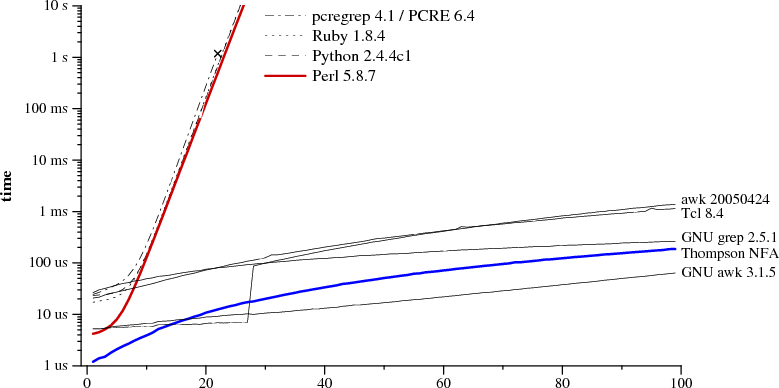
\includegraphics[width=10cm,height=7cm]{Gambar/dapi1.jpg}
\begin{equation}python regular expression\end{equation}

 \section{Berikut adalah sintaks untuk fungsi ini }
 
 \begin{itemize}
\item Fungsi Pertandingan \par
\noindent 
Fungsi ini mencoba mencocokkan pola RE dengan string dengan flag pilihan. \par
\vspace{12pt}
\noindent 

\noindent 
  \par
\noindent 

\item Parameter 
\noindent 
pattern \hspace*{0.5in}  \par
\noindent 
Ini adalah ekspresi reguler yang harus disesuaikan. \par
\vspace{12pt}
\noindent 
\item string 
\noindent 
Ini adalah string, yang akan dicari agar sesuai dengan pola pada awal string. \par
\vspace{12pt}
\noindent 
\item flags 

Anda dapat menentukan flag yang berbeda menggunakan bitwise OR ( $  \vert  $). Ini adalah pengubah, yang tercantum dalam tabel di bawah ini. \par
\vspace{12pt}
\vspace{12pt}

\item Fungsi re.match  
 
mengembalikan objek yang cocok pada kesuksesan, None on failure. Kami mengelompokkan (num) atau kelompok () fungsi objek pencocokan untuk mendapatkan ekspresi yang sesuai. \par
\noindent 


\item Match Object Methods 
 
group(num=0) \hspace*{0.5in} Metode ini mengembalikan seluruh kecocokan (atau jumlah subkelompok tertentu) \par
\vspace{12pt}
groups() \hspace*{0.5in}  \par
\noindent 
Metode ini mengembalikan semua subkelompok yang cocok dalam tupel (kosong jika tidak ada) \par
\vspace{12pt}
\vspace{12pt}
\noindent

\end{itemize} 

\begin{verbatim}
 $  \#  $! / Usr / bin / python \par
\noindent 
Impor kembali \par
\vspace{12pt}
\noindent 
Line = "Kucing lebih pintar dari pada anjing" \par
\vspace{12pt}
\noindent 
MatchObj = re.match (r '(. *) Adalah (. *?). *', Line, re.M  $  \vert  $ re.I) \par
\vspace{12pt}
\noindent 
jika cocokObj: \par
\noindent 
~~ cetak "matchObj.group ():", matchObj.group () \par
\noindent 
~~ cetak "matchObj.group (1):", matchObj.group (1) \par
\noindent 
~~ Cetak "matchObj.group (2):", matchObj.group (2) \par
\noindent 
lain: \par
\noindent 
~~ cetak "Tidak ada pertandingan !!" \par
\vspace{12pt}
\noindent 
Bila kode diatas dieksekusi, maka menghasilkan hasil sebagai berikut - \par
\vspace{12pt}
\noindent 
MatchObj.group (): Kucing lebih pintar dari pada anjing \par
\noindent 
MatchObj.group (1): Kucing \par
\noindent 
MatchObj.group (2): lebih pintar \par

\end{verbatim}

\vspace{12pt}
\section{Fungsi Pencarian} \par
\vspace{12pt}
Fungsi ini mencari kejadian pertama dari pola RE dalam string dengan flag pilihan. \par
\vspace{12pt}

\subsection{Pengertian}
Berikut adalah sintaks untuk fungsi ini: \par
\vspace{12pt}
Re.search (pola, string, flag = 0) \par
\vspace{12pt}
\noindent 
Berikut adalah deskripsi parameternya: \par
Parameter pattern Ini adalah ekspresi reguler yang harus disesuaikan. String Ini adalah string, yang akan dicari agar sesuai dengan pola di manapun dalam string. Flags Anda dapat menentukan flag yang berbeda menggunakan bitwise OR ( $  \vert  $). Ini adalah pengubah, yang tercantum dalam tabel di bawah ini.Fungsi re.search mengembalikan objek yang cocok pada kesuksesan, tidak ada yang gagal. Kami menggunakan fungsi kelompok (num) atau kelompok () dari objek pertandingan untuk mendapatkan ekspresi yang sesuai.Match Object Methods Descriptiongroup(num=0) Metode ini mengembalikan seluruh kecocokan (atau jumlah subkelompok tertentu)groups()Metode ini mengembalikan semua subkelompok yang cocok dalam tupel (kosong jika tidak ada) \par
\vspace{12pt}
\vspace{12pt}
\noindent 

\begin{verbatim}
 $  \#  $!/usr/bin/python \par
\noindent 
import re \par
\vspace{12pt}
\noindent 
line = "Cats are smarter than dogs"; \par
\vspace{12pt}
\noindent 
searchObj = re.search( r'(.*) are (.*?) .*', line, re.M $  \vert  $re.I) \par
\vspace{12pt}
\noindent 
if searchObj: \par
\noindent 
~~ print "searchObj.group() : ", searchObj.group() \par
\noindent 
~~ print "searchObj.group(1) : ", searchObj.group(1) \par
\noindent 
~~ print "searchObj.group(2) : ", searchObj.group(2) \par
\noindent 
else: \par
\noindent 
~~ print "Nothing found!!" \par
\vspace{12pt}
\noindent 
searchObj.group()~:  Cats are smarter than dogs \par
\noindent 
searchObj.group(1)~:  Cats \par
\noindent 
searchObj.group(2)~:  smarter \par
\noindent 
Pencocokan Versus Searching \par
\vspace{12pt}

\end{verbatim}



Python menawarkan dua operasi primitif yang berbeda berdasarkan ekspresi reguler: cek kecocokan untuk kecocokan hanya di awal string, sementara pencarian memeriksa kecocokan di manapun dalam string (inilah yang Perl lakukan secara default). \par
Contoh \par
\noindent 
 $  \#  $!/usr/bin/python \par
\noindent 
import re \par
\vspace{12pt}
\noindent 
line = "Cats are smarter than dogs"; \par
\vspace{12pt}
\noindent 
matchObj = re.match( r'dogs', line, re.M $  \vert  $re.I) \par
\noindent 
if matchObj: \par
\noindent 
~~ print "match --> matchObj.group() : ", matchObj.group() \par
\noindent 
else: \par
\noindent 
~~ print "No match!!" \par
\vspace{12pt}
\noindent 
searchObj = re.search( r'dogs', line, re.M $  \vert  $re.I) \par
\noindent 
if searchObj: \par
\noindent 
~~ print "search --> searchObj.group() : ", searchObj.group() \par
\noindent 
else: \par
\noindent 
~~ print "Nothing found!!" \par
\vspace{12pt}
\noindent 
No match!! \par
\noindent 
search~--> matchObj.group() :  dogs \par
\vspace{12pt}
\noindent 
Cari dan Ganti \par
\vspace{12pt}
\noindent 
Salah satu metode re yang paling penting yang menggunakan ekspresi reguler adalah sub. \par
\noindent 
Sintaksis \par
\vspace{12pt}
Re.sub (pola, repl, string, max = 0) \par
\vspace{12pt}
\noindent 
Metode ini menggantikan semua kemunculan pola RE dalam string dengan repl, mengganti semua kejadian kecuali jika max diberikan. Metode ini mengembalikan string yang dimodifikasi. \par
Contoh \par
\noindent 
 $  \#  $!/usr/bin/python \par
\noindent 
import re \par
\vspace{12pt}
\noindent 
phone = "2004-959-559  $  \#  $ This is Phone Number" \par
\vspace{12pt}
\noindent 
 $  \#  $ Delete Python-style comments \par
\noindent 
num = re.sub(r' $  \#  $.* $  \$  $', "", phone) \par
\noindent 
print "Phone Num : ", num \par
\vspace{12pt}
\noindent 
 $  \#  $ Remove anything other than digits \par
\noindent 
num~=~re.sub(r' $  \textbackslash  $D',~"", phone)     \par
\noindent 
print "Phone Num : ", num \par
\vspace{12pt}
\noindent 
Phone~Num :  2004-959-559 \par
\noindent 
Phone~Num :  2004959559 \par
\vspace{12pt}
\noindent 
Regular Expression Modifiers: Option Flags \par
Ekspresi reguler literal mungkin termasuk pengubah opsional untuk mengendalikan berbagai aspek pencocokan. Pengubah ditentukan sebagai bendera pilihan. Anda dapat memberikan beberapa pengubah menggunakan OR eksklusif ( $  \vert  $), seperti yang ditunjukkan sebelumnya dan dapat ditunjukkan oleh salah satu dari ini – Modifier Description  \par
\noindent 
re.I \hspace*{0.5in}  \par
\noindent 
Lakukan pencocokan case-insensitive. \par
\vspace{12pt}
\noindent 
re.L \hspace*{0.5in}  \par
\noindent 
Menafsirkan kata-kata sesuai dengan lokal saat ini. Interpretasi ini mempengaruhi kelompok abjad ( $  \textbackslash  $ w dan  $  \textbackslash  $ W), serta perilaku batas kata ( $  \textbackslash  $ b dan  $  \textbackslash  $ B). \par
\vspace{12pt}
\noindent 
re.M \hspace*{0.5in}  \par
\noindent 
Membuat  $  \$  $ cocok dengan akhir baris (bukan hanya akhir string) dan membuat  $  \string^  $ cocok dengan awal baris apapun (bukan hanya permulaan string). \par
\vspace{12pt}
\noindent 
re.S \hspace*{0.5in}  \par
\noindent 
Membuat sebuah periode (dot) cocok dengan karakter apapun, termasuk newline. \par
\noindent 
re.U \hspace*{0.5in}  \par
\noindent 
Menginterpretasikan huruf sesuai dengan karakter Unicode. Flag ini mempengaruhi perilaku  $  \textbackslash  $ w,  $  \textbackslash  $ W,  $  \textbackslash  $ b,  $  \textbackslash  $ B. \par
\vspace{12pt}
\noindent 
re.X \hspace*{0.5in}  \par
\noindent 
Memungkinkan sintaks ekspresi reguler "manis". Ini mengabaikan spasi (kecuali di dalam himpunan [] atau saat diloloskan oleh garis miring terbalik) dan memperlakukan unescaped  $  \#  $ sebagai tanda komentar. \par
\vspace{12pt}
\noindent 
\textbf{Pola Ekspresi Reguler} \par
\vspace{12pt}
\noindent 
Kecuali karakter kontrol, (+?.  $  \string^  $  $  \string^  $  $  \$  $ () []  $  \{  $ $  \}  $  $  \vert  $  $  \textbackslash  $), Semua karakter cocok dengan karakter mereka sendiri. Anda bisa lolos dari karakter kontrol sebelum mendahului dengan garis miring terbalik. \par
\noindent 
Berikut daftar tabel sintaks ekspresi reguler yang tersedia dengan Python - \par
\noindent 
 $  \#  $!/usr/bin/python \par
\noindent 
import re \par
\vspace{12pt}
\noindent 
phone = "2004-959-559  $  \#  $ This is Phone Number" \par
\vspace{12pt}
\noindent 
 $  \#  $ Delete Python-style comments \par
\noindent 
num = re.sub(r' $  \#  $.* $  \$  $', "", phone) \par
\noindent 
print "Phone Num : ", num \par
\vspace{12pt}
\noindent 
 $  \#  $ Remove anything other than digits \par
\noindent 
num~=~re.sub(r' $  \textbackslash  $D',~"", phone)     \par
\noindent 
print "Phone Num : ", num \par
\vspace{12pt}
\noindent 
Phone~Num :  2004-959-559 \par
\noindent 
Phone~Num :  2004959559 \par
\vspace{12pt}
\noindent 
<Directory "/var/www/cgi-bin"> \par
\noindent 
~~ AllowOverride None \par
\noindent 
~~ Options ExecCGI \par
\noindent 
~~ Order allow,deny \par
\noindent 
~~ Allow from all \par
\noindent 
</Directory> \par
\vspace{12pt}
\noindent 
<Directory "/var/www/cgi-bin"> \par
\noindent 
Options All \par
\noindent 
</Directory> \par
\vspace{12pt}
\noindent 
!/usr/bin/python \par
\vspace{12pt}
\noindent 
print "Content-type:text/html $  \textbackslash  $r $  \textbackslash  $n $  \textbackslash  $r $  \textbackslash  $n" \par
\noindent 
print '<html>' \par
\noindent 
print '<head>' \par
\noindent 
print '<title>Hello Word - First CGI Program</title>' \par
\noindent 
print '</head>' \par
\noindent 
print '<body>' \par
\noindent 
print '<h2>Hello Word! This is my first CGI program</h2>' \par
\noindent 
print '</body>' \par
\noindent 
print '</html>' \par
\vspace{12pt}
\vspace{12pt}
\noindent 
Halo kata! Ini adalah program CGI pertamaku \par
\vspace{12pt}
Script hello.py ini adalah skrip Python yang sederhana, yang menuliskan hasilnya pada file STDOUT, yaitu layar. Ada satu fitur penting dan tambahan yang tersedia yang merupakan baris pertama yang akan dicetak Content-type: text / html  $  \textbackslash  $ r  $  \textbackslash  $ n  $  \textbackslash  $ r  $  \textbackslash  $ n. Baris ini dikirim kembali ke browser dan ini menentukan jenis konten yang akan ditampilkan di layar browser. Sekarang Anda pasti sudah mengerti konsep dasar CGI dan Anda bisa menulis banyak program CGI yang rumit dengan menggunakan Python. Script ini bisa berinteraksi dengan sistem eksternal lainnya juga untuk bertukar informasi seperti RDBMS. \par
\vspace{12pt}
\vspace{12pt}
\vspace{12pt}
\vspace{12pt}
\noindent 
Header HTTP \par
\vspace{12pt}
\noindent 
Baris Content-type: text / html  $  \textbackslash  $ r  $  \textbackslash  $ n  $  \textbackslash  $ r  $  \textbackslash  $ n adalah bagian dari header HTTP yang dikirim ke browser untuk memahami isinya. Semua header HTTP akan berada dalam bentuk berikut - \par
\noindent 
 $  \#  $!/usr/bin/python \par
\vspace{12pt}
\noindent 
 $  \#  $ Import modules for CGI handling  \par
\noindent 
import cgi, cgitb  \par
\vspace{12pt}
\noindent 
 $  \#  $ Create instance of FieldStorage  \par
\noindent 
form = cgi.FieldStorage()  \par
\vspace{12pt}
\noindent 
 $  \#  $ Get data from fields \par
\noindent 
first $  \_  $name = form.getvalue('first $  \_  $name') \par
\noindent 
last $  \_  $name~ = form.getvalue('last $  \_  $name') \par
\vspace{12pt}
\noindent 
print "Content-type:text/html $  \textbackslash  $r $  \textbackslash  $n $  \textbackslash  $r $  \textbackslash  $n" \par
\noindent 
print "<html>" \par
\noindent 
print "<head>" \par
\noindent 
print "<title>Hello - Second CGI Program</title>" \par
\noindent 
print "</head>" \par
\noindent 
print "<body>" \par
\noindent 
print "<h2>Hello  $  \%  $s  $  \%  $s</h2>"  $  \%  $ (first $  \_  $name, last $  \_  $name) \par
\noindent 
print "</body>" \par
\noindent 
print "</html>" \par
\vspace{12pt}
\noindent 
<form action="/cgi-bin/hello $  \_  $get.py" method="get"> \par
\noindent 
First~Name: <input type="text" name="first $  \_  $name">  <br /> \par
\vspace{12pt}
\noindent 
Last Name: <input type="text" name="last $  \_  $name" /> \par
\noindent 
<input type="submit" value="Submit" /> \par
\noindent 
</form> \par
\vspace{12pt}
\noindent 
 $  \#  $!/usr/bin/python \par
\vspace{12pt}
\noindent 
 $  \#  $ Import modules for CGI handling  \par
\noindent 
import cgi, cgitb  \par
\vspace{12pt}
\noindent 
 $  \#  $ Create instance of FieldStorage  \par
\noindent 
form = cgi.FieldStorage()  \par
\vspace{12pt}
\noindent 
 $  \#  $ Get data from fields \par
\noindent 
first $  \_  $name = form.getvalue('first $  \_  $name') \par
\noindent 
last $  \_  $name~ = form.getvalue('last $  \_  $name') \par
\vspace{12pt}
\noindent 
print "Content-type:text/html $  \textbackslash  $r $  \textbackslash  $n $  \textbackslash  $r $  \textbackslash  $n" \par
\noindent 
print "<html>" \par
\noindent 
print "<head>" \par
\noindent 
print "<title>Hello - Second CGI Program</title>" \par
\noindent 
print "</head>" \par
\noindent 
print "<body>" \par
\noindent 
print "<h2>Hello  $  \%  $s  $  \%  $s</h2>"  $  \%  $ (first $  \_  $name, last $  \_  $name) \par
\noindent 
print "</body>" \par
\noindent 
print "</html>" \par
\vspace{12pt}
\noindent 
<form action="/cgi-bin/hello $  \_  $get.py" method="post"> \par
\noindent 
First Name: <input type="text" name="first $  \_  $name"><br /> \par
\noindent 
Last Name: <input type="text" name="last $  \_  $name" /> \par
\vspace{12pt}
\noindent 
<input type="submit" value="Submit" /> \par
\noindent 
</form> \par
\vspace{12pt}
Mari kita ambil lagi contoh yang sama seperti di atas yang melewati dua nilai menggunakan HTML FORMULIR dan tombol kirim. Kami menggunakan skrip CGI yang sama hello $  \_  $get.py untuk menangani masukan ini. \par
\noindent 
Melewati Data Kotak Centang ke Program CGI \par
\vspace{12pt}
\noindent 
Kotak centang digunakan bila lebih dari satu pilihan diperlukan untuk dipilih. \par
\vspace{12pt}
\noindent 
Berikut adalah contoh kode HTML untuk form dengan dua kotak centang - \par
\vspace{12pt}
\noindent 
Melewati Data Tombol Radio ke Program CGI \par
\vspace{12pt}
\noindent 
Tombol Radio digunakan bila hanya satu pilihan yang harus dipilih. \par
\vspace{12pt}
\noindent 
Berikut adalah contoh kode HTML untuk form dengan dua tombol radio  \par
\vspace{12pt}
\vspace{12pt}
\noindent 
 $  \#  $!/usr/bin/python \par
\vspace{12pt}
\noindent 
 $  \#  $ Import modules for CGI handling  \par
\noindent 
import cgi, cgitb  \par
\vspace{12pt}
\noindent 
 $  \#  $ Create instance of FieldStorage  \par
\noindent 
form = cgi.FieldStorage()  \par
\vspace{12pt}
\noindent 
 $  \#  $ Get data from fields \par
\noindent 
if form.getvalue('subject'): \par
\noindent 
~~ subject = form.getvalue('subject') \par
\noindent 
else: \par
\noindent 
~~ subject = "Not set" \par
\vspace{12pt}
\noindent 
print "Content-type:text/html $  \textbackslash  $r $  \textbackslash  $n $  \textbackslash  $r $  \textbackslash  $n" \par
\noindent 
print "<html>" \par
\noindent 
print "<head>" \par
\noindent 
print "<title>Radio - Fourth CGI Program</title>" \par
\noindent 
print "</head>" \par
\noindent 
print "<body>" \par
\noindent 
print "<h2> Selected Subject is  $  \%  $s</h2>"  $  \%  $ subject \par
\noindent 
print "</body>" \par
\noindent 
print "</html>" \par
\vspace{12pt}
\noindent 
<form action="/cgi-bin/textarea.py" method="post" target=" $  \_  $blank"> \par
\noindent 
<textarea name="textcontent" cols="40" rows="4"> \par
\noindent 
Type your text here... \par
\noindent 
</textarea> \par
\noindent 
<input type="submit" value="Submit" /> \par
\noindent 
</form> \par
\vspace{12pt}
\noindent 
 $  \#  $!/usr/bin/python \par
\vspace{12pt}
\noindent 
 $  \#  $ Import modules for CGI handling  \par
\noindent 
import cgi, cgitb  \par
\vspace{12pt}
\noindent 
 $  \#  $ Create instance of FieldStorage  \par
\noindent 
form = cgi.FieldStorage()  \par
\vspace{12pt}
\noindent 
 $  \#  $ Get data from fields \par
\noindent 
if form.getvalue('textcontent'): \par
\noindent 
~~ text $  \_  $content = form.getvalue('textcontent') \par
\noindent 
else: \par
\noindent 
~~ text $  \_  $content = "Not entered" \par
\vspace{12pt}
\noindent 
print "Content-type:text/html $  \textbackslash  $r $  \textbackslash  $n $  \textbackslash  $r $  \textbackslash  $n" \par
\noindent 
print "<html>" \par
\noindent 
print "<head>"; \par
\noindent 
print "<title>Text Area - Fifth CGI Program</title>" \par
\noindent 
print "</head>" \par
\noindent 
print "<body>" \par
\noindent 
print "<h2> Entered Text Content is  $  \%  $s</h2>"  $  \%  $ text $  \_  $content \par
\noindent 
print "</body>" \par
\vspace{12pt}
\noindent 
{\fontsize{14pt}{14pt}\selectfont \textbf{Menggunakan Cookies di CGI} \\} \par
\noindent 
Protokol HTTP adalah protokol tanpa kewarganegaraan. Untuk situs komersial, diperlukan informasi sesi di antara halaman yang berbeda. Misalnya, satu pendaftaran pengguna berakhir setelah menyelesaikan banyak halaman. Bagaimana cara mempertahankan informasi sesi pengguna di semua halaman web? Dalam banyak situasi, menggunakan cookies adalah metode yang paling efisien untuk mengingat dan melacak preferensi, pembelian, komisi, dan informasi lainnya yang diperlukan untuk pengalaman pengunjung atau statistik situs yang lebih baik. \par
\noindent 
Contoh dasar \par
\noindent 
Joke: apa yang kamu sebut babi dengan tiga mata? Piiig! \par
\vspace{12pt}
\noindent 
Aturan dasar pencarian ekspresi reguler untuk sebuah pola dalam sebuah string adalah: \par
\noindent 
Hasil pencarian melalui string dari awal sampai akhir, berhenti pada pertandingan pertama yang ditemukan  Semua pola harus dicocokkan, tapi tidak semua senar Jika cocok = re.search (tepuk, str) berhasil, kecocokan tidak ada dan khususnya match.group () adalah teks yang cocok \par
\vspace{12pt}
\noindent 
~  $  \#  $ $  \#  $ Search for pattern 'iii' in string 'piiig'. \par
\noindent 
~  $  \#  $ $  \#  $ All of the pattern must match, but it may appear anywhere. \par
\noindent 
~  $  \#  $ $  \#  $ On success, match.group() is matched text. \par
\noindent 
~~match = re.search(r'iii', 'piiig') =>  found, match.group() == "iii" \par
\noindent 
~~match = re.search(r'igs', 'piiig') =>  not found, match == None \par
\vspace{12pt}
\noindent 
~  $  \#  $ $  \#  $ . = any char but  $  \textbackslash  $n \par
\noindent 
~~match = re.search(r'..g', 'piiig') =>  found, match.group() == "iig" \par
\vspace{12pt}
\noindent 
~  $  \#  $ $  \#  $  $  \textbackslash  $d = digit char,  $  \textbackslash  $w = word char \par
\noindent 
~~match = re.search(r' $  \textbackslash  $d $  \textbackslash  $d $  \textbackslash  $d', 'p123g') =>  found, match.group() == "123" \par
\noindent 
~~match = re.search(r' $  \textbackslash  $w $  \textbackslash  $w $  \textbackslash  $w', '@@abcd!!') =>  found, match.group() == "abc" \par
\vspace{12pt}
\vspace{12pt}
\noindent 
Pengulangan \par
\vspace{12pt}
\noindent 
Hal menjadi lebih menarik saat Anda menggunakan + dan * untuk menentukan pengulangan dalam polanya \par
\vspace{12pt}
\noindent 
~~~ + - 1 atau lebih kemunculan pola ke kiri, mis. 'I +' = satu atau lebih i's \par
\noindent 
~~~ * - 0 atau lebih kemunculan pola ke kiri \par
\noindent 
~~~ ? - cocokkan 0 atau 1 kemunculan pola ke kiri \par
\vspace{12pt}
\vspace{14pt}
\noindent 
{\fontsize{14pt}{14pt}\selectfont \textbf{Paling kiri  $  \&  $ terbesar} \\} \par
Pertama, pencarian menemukan kecocokan paling kiri untuk pola tersebut, dan kedua mencoba menggunakan sebanyak mungkin string - yaitu + dan * sejauh mungkin (huruf + dan * dikatakan "serakah"). \par
\noindent 
Contoh pengulangan \par
\vspace{12pt}
\noindent 
 $  \#  $ $  \#  $ i+ = one or more i's, as many as possible. \par
\noindent 
~~match = re.search(r'pi+', 'piiig') =>  found, match.group() == "piii" \par
\vspace{12pt}
\noindent 
~  $  \#  $ $  \#  $ Finds the first/leftmost solution, and within it drives the + \par
\noindent 
~  $  \#  $ $  \#  $ as far as possible (aka 'leftmost and largest'). \par
\noindent 
~  $  \#  $ $  \#  $ In this example, note that it does not get to the second set of i's. \par
\noindent 
~~match = re.search(r'i+', 'piigiiii') =>  found, match.group() == "ii" \par
\vspace{12pt}
\noindent 
~  $  \#  $ $  \#  $  $  \textbackslash  $s* = zero or more whitespace chars \par
\noindent 
~  $  \#  $ $  \#  $ Here look for 3 digits, possibly separated by whitespace. \par
\noindent 
~~match~=~re.search(r' $  \textbackslash  $d $  \textbackslash  $s* $  \textbackslash  $d $  \textbackslash  $s* $  \textbackslash  $d',~'xx1~2   3xx') =>  found, match.group() == "1 2   3" \par
\noindent 
~~match~=~re.search(r' $  \textbackslash  $d $  \textbackslash  $s* $  \textbackslash  $d $  \textbackslash  $s* $  \textbackslash  $d', 'xx12  3xx') =>  found, match.group() == "12  3" \par
\noindent 
~~match = re.search(r' $  \textbackslash  $d $  \textbackslash  $s* $  \textbackslash  $d $  \textbackslash  $s* $  \textbackslash  $d', 'xx123xx') =>  found, match.group() == "123" \par
\vspace{12pt}
\noindent 
~  $  \#  $ $  \#  $  $  \string^  $ = matches the start of string, so this fails: \par
\noindent 
~~match = re.search(r' $  \string^  $b $  \textbackslash  $w+', 'foobar') =>  not found, match == None \par
\noindent 
~  $  \#  $ $  \#  $ but without the  $  \string^  $ it succeeds: \par
\noindent 
~~match = re.search(r'b $  \textbackslash  $w+', 'foobar') =>  found, match.group() == "bar" \par
\vspace{12pt}
\vspace{12pt}
\noindent 
{\fontsize{14pt}{14pt}\selectfont \textbf{Contoh email} \\} \par
Misalkan Anda ingin mencari alamat email di dalam string 'xyz alice-b@google.com ungu monyet'. Kami akan menggunakan ini sebagai contoh yang berjalan untuk menunjukkan fitur ekspresi reguler. Berikut adalah upaya menggunakan pola r ' $  \textbackslash  $ w + @  $  \textbackslash  $ w +': \par
\vspace{12pt}
\noindent 
~ Str = 'ungu alice-b@google.com monyet pencuci piring' \par
\noindent 
~ Match = re.search (r ' $  \textbackslash  $ w + @  $  \textbackslash  $ w +', str) \par
\noindent 
~ Jika cocok: \par
\noindent 
~~~ print match.group ()  $  \#  $ $  \#  $ 'b @ google' \par
\vspace{12pt}
Pencarian tidak mendapatkan keseluruhan alamat email dalam kasus ini karena  $  \textbackslash  $ w tidak cocok dengan '-' atau '.' Di alamat Kami akan memperbaikinya menggunakan fitur ekspresi reguler di bawah ini. Kurung persegi Tanda kurung siku dapat digunakan untuk menunjukkan sekumpulan karakter, jadi [abc] cocok dengan 'a' atau 'b' atau 'c'. Kode  $  \textbackslash  $ w,  $  \textbackslash  $ s dll bekerja di dalam kurung siku juga dengan satu pengecualian bahwa titik (.) Hanya berarti titik literal. Untuk masalah email, tanda kurung siku adalah cara mudah untuk menambahkan '.' Dan '-' ke kumpulan karakter yang dapat muncul di sekitar @ dengan pola r '[ $  \textbackslash  $ w .-] + @ [ $  \textbackslash  $ w .-] +' untuk mendapatkan keseluruhan alamat email: \par
\vspace{12pt}
\noindent 
~ Match = re.search (r '[ $  \textbackslash  $ w .-] + @ [ $  \textbackslash  $ w .-] +', str) \par
\noindent 
~ Jika cocok: \par
\noindent 
~~~ print match.group ()  $  \#  $ $  \#  $ 'alice-b@google.com' \par
\vspace{12pt}
(Lebih banyak fitur kotak-braket) Anda juga dapat menggunakan tanda hubung untuk menunjukkan jangkauan, jadi [a-z] cocok dengan semua huruf kecil. Untuk menggunakan tanda hubung tanpa menunjukkan jangkauan, pasang tanda hubung terakhir, mis. [abc-]. Top-up ( $  \string^  $) pada awal set persegi-braket telah membalikkannya, jadi [ $  \string^  $ ab] berarti karakter apapun kecuali 'a' atau 'b'. \par
\vspace{16pt}
{\fontsize{14pt}{14pt}\selectfont \textbf{Ekstraksi Grup} \\} \par
Fitur "kelompok" dari ekspresi reguler memungkinkan Anda untuk memilih bagian dari teks yang sesuai. Misalkan untuk masalah email yang ingin kita ekstrak username dan host secara terpisah. Untuk melakukan ini, tambahkan kurung () di sekitar nama pengguna dan host dalam pola, seperti ini: r '([ $  \textbackslash  $ w .-] +) @ ([ $  \textbackslash  $ w .-] +)'. Dalam kasus ini, tanda kurung tidak mengubah pola yang akan cocok, sebaliknya mereka membentuk "kelompok" logis dalam teks pertandingan. Pada pencarian yang sukses, match.group (1) adalah teks kecocokan yang sesuai dengan tanda kurung kiri ke 1, dan match.group (2) adalah teks yang sesuai dengan kurung kiri ke-2. Match.group polos () masih merupakan keseluruhan teks pertandingan seperti biasa. \par
\vspace{12pt}
\noindent 
~ Str = 'ungu alice-b@google.com monyet pencuci piring' \par
\noindent 
~ Match = re.search ('([ $  \textbackslash  $ w .-] +) @ ([ $  \textbackslash  $ w .-] +)', str) \par
\noindent 
~ Jika cocok: \par
\noindent 
~~~ Print match.group ()  $  \#  $ $  \#  $ 'alice-b@google.com' (keseluruhan pertandingan) \par
\noindent 
~~~ Print match.group (1)  $  \#  $ $  \#  $ 'alice-b' (nama pengguna, grup 1) \par
\noindent 
~~~ Print match.group (2)  $  \#  $ $  \#  $ 'google.com' (host, grup 2) \par
\vspace{12pt}
Alur kerja umum dengan ekspresi reguler adalah Anda menulis sebuah pola untuk hal yang Anda cari, menambahkan kelompok tanda kurung untuk mengekstrak bagian yang Anda inginkan. Temukan semua Findall () mungkin adalah fungsi tunggal yang paling kuat dalam modul re. Di atas kami menggunakan re.search () untuk menemukan kecocokan pertama untuk sebuah pola. Findall () menemukan * semua * kecocokan dan mengembalikannya sebagai daftar string, dengan masing-masing string mewakili satu kecocokan. \par
\vspace{12pt}
\vspace{12pt}
\noindent 
~  $  \#  $ $  \#  $ Misalkan kita memiliki teks dengan banyak alamat email \par
\noindent 
~ Str = 'ungu alice@google.com, bla monyet bob@abc.com blah pencuci piring' \par
\vspace{12pt}
\noindent 
~  $  \#  $ $  \#  $ disini re.findall () mengembalikan daftar semua string email yang ditemukan \par
\noindent 
~ Email = re.findall (r '[ $  \textbackslash  $ w  $  \textbackslash  $ .-] + @ [ $  \textbackslash  $ w  $  \textbackslash  $ .-] +', str)  $  \#  $ $  \#  $ ['alice@google.com', 'bob@abc.com'] \par
\noindent 
~ Untuk email di email: \par
\noindent 
~~~  $  \#  $ Lakukan sesuatu dengan setiap string email yang ditemukan \par
\noindent 
~~~ Cetak email \par
\vspace{12pt}



\chapter{Networking}

Aditya Pratama 
Bendra Wardhana 
Andi Syahjaratu
Dini Islamiani
Nur Rahmawati

%kelompok 4 D4 TI-2D
%Ayu Permata Sari        1154022
%Librantara Erlangga     1154071
%Martin Luter Zega       1154120
%Putri Aulia Ramadhanie  1154096
%Ryan Hafizh Herdiana    1154067

\section{Pengertian Jaringan}
  Jaringan yaitu sekumpulan komputer yang dihubungkan dengan kabel sehingga komputer yang satu dengan komputer yang lainnya dapat saling komunikasi, bertukar informasi sharing file, printer, dan sebagainya.
  Networking merupakan salah satu cabang ilmu dunia Teknik Informatika yang membahas tentang komunikasi antar komputer. Materi networking yang di berikan di sekolah atau di perkuliahan saat ini sepertinya belum cukup memadai dari yang diharapkan. Bagi mereka yang sangat ingin mendalami tentang ilmu networking bisa mempelajarinya dari artikel-artikel di internet, dan biasanya ketika kita menemukan artikel tentang materi networking yang ingin dipelajari sering sekali ditemukan kata-kata atau istilah-istilah yang belum dimengerti, biasanya kita akan mencari kata-kata tersebut dengan mengetikkan keywordnya di mesin pencari Google. lalu kita akan belajar memahami kata tersebut, setelah kita mengerti kita akan kembali mempelajari materi yang tadi. cara ini tentu tidak efektif. maka dari sebaiknya sebelum kita mempelajari mengenai networking kita pelajari dulu dari yang paling dasar, yaitu istilah-istilah dalam networking.
  Networking sangat dibutuhkan, terutama pada zaman yang semakin lama semakin canggih seperti ini, karena jaringan itu tentu sangat penting untuk berlangsungnya hubungan atau komunikasi antar komputer. Misalnya saja untuk berbagi atau sharing printer, tidak mungkin setiap komputer memiliki printer satu-satu makannya dibuatlah jaringan komputer itu untuk berbagi penggunaan printer secara bersama-sama dan juga berfungsi untuk sharing internet, satu komputer (server) dapat ip address dari isp, lalu si server itu membagikan koneksi internet ke client-client dikantornya.

\section{Jenis-Jenis Jaringan berdasarkan jangkuan}
  \subsection{Local Area Networking (LAN)}
    Yaitu Jaringan yang dibatasi oleh area yang relative kecil, umumnya dibatasi oleh area lingkungan seperti sebuah perkantoran di sebuah gedung, atau sebuah sekolah, dan biasanya tidak jauh dari sekitar 1 km persegi.
  \subsection{Metropolitan Area Networking (MAN)}
    Yaitu Jaringan yang lebih luas dari LAN, MAN biasanya meliputi area yang lebih besar seperti area propinsi, antar gedung. Mengapa MAN itu dikatakan lebih luas dari LAN?, Yah, karena jaringan MAN itu terhubung dari beberapa jaringan LAN yang dihubungkan melalui switch lagi.
  \subsection{Wide Area Networking (WAN)}
    Yaitu Jaringan yang lingkupnya biasanya sudah menggunakan sarana Satelit ataupun kabel bawah laut sebagai contoh keseluruhan jaringan BANK BNI yang ada di Indonesia ataupun yang ada di Negara-negara lain. Menggunakan sarana WAN, Sebuah Bank yang ada di Bandung bisa menghubungi kantor cabangnya yang ada di Hongkong, hanya dalam beberapa menit. Biasanya WAN agak rumit dan sangat kompleks, menggunakan banyak sarana untuk menghubungkan antara LAN dan WAN ke dalam Komunikasi Global seperti Internet.

\section{Manfaat Jaringan Komputer}
  Berbicara mengenai manfaat dari jaringan komputer. Terdapat banyak sekali manfaat jaringan komputer, antara lain :
    \begin{enumerate}
      \item Dengan jaringan komputer, kita bisa mengakses file yang kita miliki sekaligus file orang lain yang telah diseberluaskan melalui suatu jaringan, semisal jaringan internet.
      \item Melalui jaringan komputer, kita bisa melakukan proses pengiriman data secara cepat dan efisien.
      \item Jaringan komputer membantu seseorang berhubungan dengan orang lain dari berbagai negara dengan mudah.
      \item Selain itu, pengguna juga dapat mengirim teks, gambar, audio, maupun video secara real time dengan bantuan jaringan komputer.
      \item Kita dapat mengakses berita atau informasi dengan sangat mudah melalui internet dikarenakan internet merupakan salah satu contoh jaringan komputer.
    \end{enumerate}

\section{Macam-Macam Jaringan Komputer}
  Umumnya jaringan komputer di kelompokkan menjadi 5 kategori, yaitu berdasarkan jangkauan geografis, distribusi sumber informasi/ data, media transmisi data, peranan dan hubungan tiap komputer dalam memproses data, dan berdasarkan jenis topologi yang digunakan. Berikut penjabaran lengkapnya :
  \subsection{A. Berdasarkan Jangkauan Geografis}

    \subsubsection{LAN} 
      Local Area Network atau yang sering disingkat dengan LAN merupakan jaringan yang hanya mencakup wilayah kecil saja, semisal warnet, kantor, atau sekolah. Umumnya jaringan LAN luas areanya tidak jauh dari 1 km persegi.
    Biasanya jaringan LAN menggunakan teknologi IEEE 802.3 Ethernet yang mempunyai kecepatan transfer data sekitar 10, 100, bahkan 1000 MB/s. Selain menggunakan teknologi Ethernet, tak sedikit juga yang menggunakan teknologi nirkabel seperti Wi-fi untuk jaringan LAN.
    Keuntungan dari penggunaan Jenis Jaringan Komputer LAN seperti lebih irit dalam pengeluaran biaya operasional, lebih irit dalam penggunaan kabel, transfer data antar node dan komputer labih cepat karena mencakup wilayah yang sempit atau lokal, dan tidak memerlukan operator telekomunikasi untuk membuat sebuah jaringan LAN.
    Kerugian dari penggunaan Jenis Jaringan LAN adalah cakupan wilayah jaringan lebih sempit sehingga untuk berkomunikasi ke luar jaringan menjadi lebih sulit dan area cakupan transfer data tidak begitu luas.
    Berbeda dengan Jaringan Area Luas atau Wide Area Network(WAN), maka LAN mempunyai karakteristik sebagai berikut:

    \begin{enumerate}
    \item Mempunyai pesat data yang lebih tinggi.
    \item Meliputi wilayah geografi yang lebih sempit.
    \item Tidak membutuhkan jalur telekomunikasi yang disewa dari dari operator telekomunikasi.
    \end{enumerate}

    \subsubsection{MAN}
      Metropolitan Area Network atau MAN merupakan jaringan yang mencakup suatu kota dengan dibekali kecepatan transfer data yang tinggi. Bisa dibilang, jaringan MAN merupakan gabungan dari beberapa jaringan LAN.
    Jangakauan dari jaringan MAN berkisar 10-50 km. MAN hanya memiliki satu atau dua kabel dan tidak dilengkapi dengan elemen switching yang berfungsi membuat rancangan menjadi lebih simple.
    Keuntungan dari Jenis Jaringan Komputer MAN ini diantaranya adalah cakupan wilayah jaringan lebih luas sehingga untuk berkomunikasi menjadi lebih efisien, mempermudah dalam hal berbisnis, dan juga keamanan dalam jaringan menjadi lebih baik.
    Kerugian dari Jenis Jaringan Komputer MAN seperti lebih banyak menggunakan biaya operasional, dapat menjadi target operasi oleh para Cracker untuk mengambil keuntungan pribadi, dan untuk memperbaiki jaringan MAN diperlukan waktu yang cukup lama.
    \subsubsection{WAN}
      Wide Area Network atau WAN merupakan jaringan yang jangkauannya mencakup daerah geografis yang luas, semisal sebuah negara bahkan benua. WAN umumnya digunakan untuk menghubungkan dua atau lebih jaringan lokal sehingga pengguna dapat berkomunikasi dengan pengguna lain meskipun berada di lokasi yang berbebeda.
    Keuntungan Jenis Jaringan Komputer WAN seperti cakupan wilayah jaringannya lebih luas dari Jenis Jaringan Komputer LAN dan MAN, tukar-menukar informasi menjadi lebih rahasia dan terarah karena untuk berkomunikasi dari suatu negara dengan negara yang lainnya memerlukan keamanan yang lebih, dan juga lebih mudah dalam mengembangkan serta mempermudah dalam hal bisnis.
    Kerugian dari Jenis Jaringan WAN seperti biaya operasional yang dibutuhkan menjadi lebih banyak, sangat rentan terhadap bahaya pencurian data-data penting, perawatan untuk jaringan WAN menjadi lebih berat.

\subsection{B. Berdasarkan Distribusi Sumber Informasi/Data}
  \subsubsection{Jaringan Terpusat}
  Yang dimaksud jaringan terpusat adalah jaringan yang terdiri dari komputer client dan komputer server dimana komputer client bertugas sebagai perantara dalam mengakses sumber informasi/ data yang berasal dari komputer server. Dalam jaringan terpusat, terdapat istilah dumb terminal (terminal bisu), dimana terminal ini tidak memiliki alat pemroses data.
  \subsubsection{ Jaringan Terdistribusi}
  Jaringan ini merupakan hasil perpaduan dari beberapa jaringan terpusat sehingga memungkinkan beberapa komputer server dan client yang saling terhubung membentuk suatu sistem jaringan tertentu.
\subsection{C. Berdasarkan Media Transmisi Data yang Digunakan}
  \subsubsection{Jaringan Berkabel (Wired Network)}
    Media transmisi data yang digunakan dalam jaringan ini berupa kabel. Kabel tersebut digunakan untuk menghubungkan satu komputer dengan komputer lainnya agar bisa saling bertukar informasi/ data atau terhubung dengan internet. Salah satu media transmisi yang digunakan dalam wired network adalah kabel UTP.
  \subsubsection{ Jaringan Nirkabel (Wireless Network)}
    Dalam jaringan ini diperlukan gelombang elektromagnetik sebagai media transmisi datanya. Berbeda dengan jaringan berkabel (wired network), jaringan ini tidak menggunakan kabel untuk bertukar informasi/ data dengan komputer lain melainkan menggunakan gelombang elektromagnetik untuk mengirimkan sinyal informasi/ data antar komputer satu dengan komputer lainnya. Wireless adapter, salah satu media transmisi yang digunakan dalam wireless network.
\subsection{D. Berdasarkan Peranan dan Hubungan Tiap Komputer dalam Memproses Data}
  \subsubsection{ Jaringan Client-Server}
    Jaringan ini terdiri dari satu atau lebih komputer server dan komputer client. Biasanya terdiri dari satu komputer server dan beberapa komputer client. Komputer server bertugas menyediakan sumber daya data, sedangkan komputer client hanya dapat menggunakan sumber daya data tersebut.
  \subsubsection{ Jaringan Peer to Peer}
    Dalam jaringan ini, masing-masing komputer, baik itu komputer server maupun komputer client mempunyai kedudukan yang sama. Jadi, komputer server dapat menjadi komputer client, dan sebaliknya komputer client juga dapat menjadi komputer server.
\subsection{E. Berdasarkan Topologi Jaringan yang Digunakan}
  Topologi jaringan adalah bentuk perancangan baik secara fisik maupun secara logik yang digunakan untuk membangun sebuah jaringan komputer. rancangan ini sangat erat kaitannya dengan metode access dan media pengiriman yang digunakan. Topologi yang ada sangatlah tergantung dengan letak geofrapis dari masing-masing terminal, kualitas kontrol yang dibutuhkan dalam komunikasi ataupun penyampaian pesan, serta kecepatan dari pengiriman data.
  \subsubsection{Topologi Bus}
    \ref{bus}
  	\begin{figure}[ht]
  	\centerline{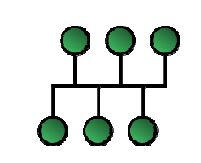
\includegraphics[width=1\textwidth]{figures/bus.JPG}}
  	\caption{Topologi bus.}
  	\label{bus}
  	\end{figure}
    Gambar ini \ref{bus} adalah topologi bus,berdasarkan artikel yudianto Topologi bus merupakan topologi yang banyak digunakan pada masa penggunaan kabel sepaksi menjamur\cite{yudianto2007jaringan}. Dengan menggunakan T-Connector(dengan terminator 50ohm pada ujung network), maka komputer atau perangkat jaringan lainnya bisa dengan mudah dihubungkan satu sama lain.
  Kesulitan utama dari penggunaan kabel sepaksi adalah sulit uuntuk mengukur apakah kabel sepakksi yang di gunakan benar-benar matching atau tidak. Karena kalau tidak sungguh-sungguh diukur secara benar akan merusak NIC yang digunakan dan kinerja jaringan menjadi terhambat, tidak mencapai kemampuan maksimalnya. Topologi ini juga sering digunakan pada jaringan dengan basis FO.
  \subsubsection{Topologi Star}
    \ref{star}
    \begin{figure}[ht]
    \centerline{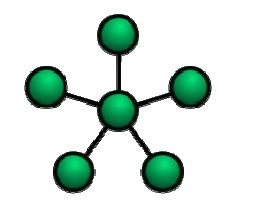
\includegraphics[width=1\textwidth]{figures/star.JPG}}
    \caption{Topologi star.}
    \label{star}
    \end{figure}
    Gambar ini \ref{star} adalah topologi star,berdasarkan artikel tudianto Topologi bintang merupakan bentuk topologi jaringan yang berupa konvergensi dari node tengah ke setiap node atau pengguna\cite{yudianto2007jaringan}. Topologi jaringan bintang termasuk topologi jaringan dengan biaya menengah.
  \subsubsection{Topologi Ring}
    \ref{ring}
    \begin{figure}[ht]
    \centerline{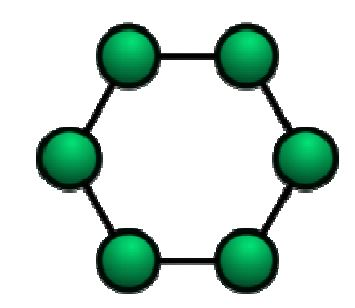
\includegraphics[width=1\textwidth]{figures/ring.JPG}}
    \caption{Topologi ring.}
    \label{ring}
    \end{figure}
    Gambar ini \ref{ring} adalah topologi ring/cincin,berdasarkan artikel yudianto Topologi cincin adalah topologi jaringan berbentuk rangkaian titik yang masing-masing terhubung ke dua titik lainnya, sedemikian sehingga membentuk jalur melingkar membentuk cincin\cite{yudianto2007jaringan}. Pada Topologi cincin,masing - masing titik/node berfungsi sebagai repeater yang akan memperkuat sinyal disepanjang sirkulasinya, artinya masing - masing perangkat saling bekerjasama untuk menerima sinyal dari perangkat sebelumnya kemudian meneruskannya pada perangkat sesudahnya, proses menerima dan meneruskan sinyal data ini dibantu oleh TOKEN. TOKEN berisi informasi bersamaan dengan data yang berasal dari komputer sumber, token kemudian akan melewati titik/node dan akan memeriksa apakah informasi data tersebut digunakan oleh titik/node yang bersangkutan, jika ya maka token akan memberikan data yang diminta oleh node untuk kemudian kembali berjalan ke titik/node berikutnya dalam jaringan. Jika tidak maka token akan melewati titik/node sambil membawa data menuju ke titik/node berikutnya. proses ini akan terus berlangsung hingga sinyal data mencapai tujuannya.
  \subsubsection{Topologi Mesh}
    \ref{mesh}
    \begin{figure}[ht]
    \centerline{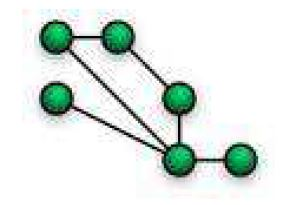
\includegraphics[width=1\textwidth]{figures/mesh.JPG}}
    \caption{Topologi mesh.}
    \label{mesh}
    \end{figure}

    Gambar ini \ref{mesh} adalah topologi mesh, berdasarkan artikel dari yudianto Topologi mesh adalah suatu bentuk hubungan antar perangkat dimana setiap perangkat terhubung secara langsung ke perangkat lainnya yang ada di dalam jaringan\cite{yudianto2007jaringan}. Akibatnya, dalam topologi mesh setiap perangkat dapat berkomunikasi langsung dengan perangkat yang dituju (dedicated links). Dengan demikian maksimal banyaknya koneksi antar perangkat pada jaringan bertopologi mesh ini dapat dihitung yaitu sebanyak \begin{equation}n(n-1)/2\end{equation}. 
    Selain itu karena setiap perangkat dapat terhubung dengan perangkat lainnya yang ada di dalam jaringan maka setiap perangkat harus memiliki sebanyak n-1 Port Input/Output (I/O ports).Berdasarkan pemahaman di atas, dapat dicontohkan bahwa apabila sebanyak 5(lima) komputer akan dihubungkan dalam bentuk topologi mesh maka agar seluruh koneksi antar komputer dapat berfungsi optimal, diperlukan kabel koneksi sebanyak \begin{verbatim}5(5-1)/2 = 10 \end{verbatim} kabel koneksi, dan masing-masing komputer harus memiliki port I/O sebanyak 5-1 = 4 port.
  \subsubsection{Topologi Tree}
    \ref{tree}
    \begin{figure}[ht]
    \centerline{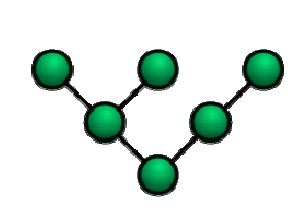
\includegraphics[width=1\textwidth]{figures/tree.JPG}}
    \caption{Topologi tree.}
    \label{tree}
    \end{figure}
    Gambar ini \ref{tree} adalah topologi tree, berdasarkan artikel dari yudianto Topologi Pohon adalah kombinasi karakteristik antara topologi bintang dan topologi bus\cite{yudianto2007jaringan}. Topologi ini terdiri atas kumpulan topologi bintang yang dihubungkan dalam satu topologi bus sebagai jalur tulang punggung atau backbone. Komputer-komputer dihubungkan ke hub, sedangkan hub lain di hubungkan sebagai jalur tulang punggung.Topologi jaringan ini disebut juga sebagai topologi jaringan bertingkat. Topologi ini biasanya digunakan untuk interkoneksi antar sentral dengan hirarki yang berbeda. Untuk hirarki yang lebih rendah digambarkan pada lokasi yang rendah dan semakin keatas mempunyai hirarki semakin tinggi. Topologi jaringan jenis ini cocok digunakan pada sistem jaringan komputer.Pada jaringan pohon, terdapat beberapa tingkatan simpul atau node.Pusat atau simpul yang lebih tinggi tingkatannya, dapat mengatur simpul lain yang lebih rendah tingkatannya. Data yang dikirim perlu melalui simpul pusat terlebih dahulu. Misalnya untuk bergerak dari komputer dengan node-3 kekomputer node-7 seperti halnya pada gambar, data yang ada harus melewati node-3, 5 dan node-6 sebelum berakhir pada node-7.
  \subsubsection{Topologi Linier}
    \ref{linier}
    \begin{figure}[ht]
    \centerline{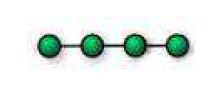
\includegraphics[width=1\textwidth]{figures/linier.JPG}}
    \caption{Topologi linier.}
    \label{linier}
    \end{figure}
    Gambar ini \ref{linier} adalah topologi linier, Topologi ini biasa disebut dengan topologi bus beruntut, tata letak ini termasuk tata letak umum.

\section{Alat-alat jaringan}
Macam-macam alat jaringan antara lain :
  \subsection{ROUTER}
    Router adalah sebuah alat yang mengirimkan paket data melalui sebuah jaringan atau Internet menuju tujuannya, alat ini sangatlah penting untuk meneruskan jaringan satu ke jaringan lainnya yang berbeda kelas/subnet/ip. melalui sebuah proses yang dikenal sebagai routing. Proses routing terjadi pada lapisan 3 (Lapisan jaringan seperti Internet Protocol) dari stack protokol tujuh-lapis OSI.
  Router berfungsi sebagai penghubung antar dua atau lebih jaringan untuk meneruskan data dari satu jaringan ke jaringan lainnya. Router berbeda dengan switch. Switch merupakan penghubung beberapa alat untuk membentuk suatu Local Area Network (LAN).
  \subsection{SWITCH}
    Switch adalah perangkat jaringan komputer yang bekerja di OSI Layer 2, Data Link Layer. Switch kerjanya sebagai penyambung atau concentrator dalam Jaringan komputer. Switch mengenal MAC Adressing shingga dia bisa memilah paket data mana yang akan di teruskan/dilanjutkan ke mana.
\subsection{ACCESS POINT}
    Access point adalah perangkat yang digunakan sebagai pembuat koneksi wireless pada jaringan komputer. Fungsi Access point diantaranya: Sebagai perangkat jaringan yang berfungsi membuat jaringan komputer tanpa kabel, atau biasa disebut WI-FI (Wireless Fidelity)
  Belajar Network Programming pada python, melalui fungsi-fungsi TCP/IP, SOCKET, dll.

\section{Latihan Jaringan pada python}
Pada latihan ini, kita akan mencoba mengirim data dari server menuju klien dengan menggunakan Socket pada python.
\subsection{server.py}
Penjelasan fungsi-fungsi tsb akan dijelaskan dibawah ini:
\begin{enumerate}
 \item socket.socket(): Membuat socket baru menggunakan alamat yang sudah ada, tipe socket, dan nomor protocol.
 \item socket.bind(address): Menyalin/mengikat socket ke alamat yang ada.
 \item socket.listen(backlog): Menunggu koneksi yang sudah dibuat dari socket tersebut. backlog merupakan sebuah argumen yang menyatakan batas maximal nomor antrian koneksi dan paling tidak sampai dengan 0; nilai maximum tergantung dari sistem(biasanya 5), dan nilai minimumnya harus mencapai 0.
 \item socket.accept(): Nilai yang dikembalikan atau diberikan adalah sepasang(conn, address) dimana conn adalah socket baru yaitu sebuah objek yang biasa digunakan untuk mengirim dan menerima data dari koneksi tersebut dan address adalah alamat yang terikat ke socket pada akhir koneksi.
 \item socket.send(bytes[, flags]): Mengiri data ke socket. Socket harus terkoneksi oleh remote Socket. mengembalikan angkat dari bytes yang terkirim. Aplikasi yang bertugas untuk mengecek semua data harus terkirim; hanya jika data ditransimisikan, aplikasi membutuhkan usaha untuk mengirimkan data yang tersisa.
 \item socket.close(): Menandakan bahwa socket telah ditutup. semua dari operasi-operasi pada objek socket akan gagal. Remote End tidak akan menerima data lagi (sampai data telah dibersihkan). Socket-socket secara otomatis tertutup ketika dilakukan garbage-collected, tetapi lebih baik untuk close() mereka secara eksplisit.
\end{enumerate}
Sebelumnya pesan diatas tidak akan muncul sebelum kita menjalankan script client.py pada tab terminal lain.
maka setiap kali kita menjalankan script client.py akan terus mengirimkan pesan kepada server maupun client.

contoh networking:
\begin{verbatim}
192.168.0.0/24 subnet mask 255.255.255.0, 256 IP rumus-nya

(jumlah IP network diatas / 2) + (subnetmask diatasnya)= subnetmask yang digunakan

(256/2) + n = 128, jadi subnet mask buat 128 ip adalah 255.255.255.128
(128/2) + 128 = 192, jadi subnetmask buat 64 ip adalah 255.255.255.192
(64/2) + 192 = 224, jadi subnet mask buat 32 ip adalah 255.255.255.224
(32/2) + 224 = 240, jadi subnet mask buat 16 ip adalah 255.255.255.240
(16/2) + 240 = 248, jadi subnet mask buat 8 ip adalah 255.255.255.248
(8/2) + 248 = 252, jadi subnet mask buat 4 ip adalah 255.255.255.252
(4/2) + 252 = 254, jadi subnet mask buat 2 ip adalah 255.255.255.254
(2/2) + 254 = 255, jadi subnet mask buat 1 ip adalah 255.255.255.255
\end{verbatim}



\chapter{CGI Programming}
\section{Common Gateway Interface}
\subsection{Sejarah Common Gateway Interface}
Pada tahun 1993, tim National Center for Supercomputing Applications (NCSA) menulis spesifikasi untuk memanggil executable command line di milis www-talk. [2] [3] [4] Pengembang server Web lainnya menggunakannya, dan telah menjadi standar untuk server Web sejak saat itu. Sebuah kelompok kerja yang dipimpin oleh Ken Coar dimulai pada bulan November 1997 untuk mendapatkan definisi NCSA tentang CGI yang lebih formal. [5] Karya ini menghasilkan RFC 3875, yang menentukan Versi CGI 1.1. Secara khusus disebutkan di RFC adalah kontributor berikut: [6]
\begin{itemize}
\item Rob McCool (penulis Server Web HTTP NCSA)
\item John Franks (penulis GN Web Server)
\item Ari Luotonen (pengembang CERN httpd Web Server)
\item Tony Sanders (penulis Web Server Plexus)
\item George Phillips (pengelola server Web di University of British Columbia)
\end{itemize}
Secara historis skrip CGI sering ditulis menggunakan bahasa C. RFC 3875 Common Gateway Interface (CGI) secara parsial mendefinisikan CGI menggunakan C, [7] seperti dalam mengatakan bahwa variabel lingkungan ``diakses oleh perpustakaan perpustakaan umum getenv () atau variabel lingkungan``. 
\subsection{Common Gateway Interface}
Common Gateway Interface atau disingkat CGI merupakan standar untuk menghubungkan berbagai program aplikasi ke halaman web. CGI mirip dengan program komputer yang menjadi perantara antara standar HTML yang menjadikan tampilan web dengan program lain, seperti basis data (database). Hasil yang diperoleh dari proses pencarian dikirimkan kembali ke halaman web untuk ditampilkan dalam format HTML. CGI (Common Gateway Interface) adalah bentuk dari hubungan interaktif di mana client (browser) bisa mengirimkan suatu masukan kepada server, dan server mengolah masukan tersebut serta mengembalikannya kepada client (browser). Contoh sederhana adalah saat kita menggunakan sebuah mesin pencari. Saat kita menuliskan keyword dan menekan tombol Search maka browser akan mengirimkan keyword tersebut ke server. Keyword tersebut lalu diolah oleh server dan server mengirimkan data hasil pengolahan (yang sesuai dengan keyword yang kita masukkan) ke browser kita. Jadi yang akan kita lihat pada browser adalah  hanya data yang sesuai dengan keyword yang kita masukkan. 
\subsection{Common Gateway Interface}
Common Gateway Interface atau disingkat CGI merupakan standar untuk menghubungkan berbagai program aplikasi ke halaman web. CGI mirip dengan program komputer yang menjadi perantara antara standar HTML yang menjadikan tampilan web dengan program lain, seperti basis data (database). Hasil yang diperoleh dari proses pencarian dikirimkan kembali ke halaman web untuk ditampilkan dalam format HTML. CGI (Common Gateway Interface) adalah bentuk dari hubungan interaktif di mana client (browser) bisa mengirimkan suatu masukan kepada server, dan server mengolah masukan tersebut serta mengembalikannya kepada client (browser). Contoh sederhana adalah saat kita menggunakan sebuah mesin pencari. Saat kita menuliskan keyword dan menekan tombol Search maka browser akan mengirimkan keyword tersebut ke server. Keyword tersebut lalu diolah oleh server dan server mengirimkan data hasil pengolahan (yang sesuai dengan keyword yang kita masukkan) ke browser kita. Jadi yang akan kita lihat pada browser adalah  hanya data yang sesuai dengan keyword yang kita masukkan. 
Untuk dapat menggunakan CGI syarat yang utama adalah server dengan sistem operasi UNIX (beserta variantnya). Namun perlu kita perhatikan bahwa tidak semua server UNIX (gratis) mampu menangani dan melayani CGI. Server-server yang melayani penempatan web yang berlayanan gratis seperti Geocities dan Homepage, tidak akan mengijinkan penggunaan script CGI dalam web kita. Untuk itu kita bisa mencoba Virtual Avenue, Tripod, atau Hypermart.
	Program CGI ditulis dengan menggunakan bahasa yang dapat dimengerti oleh sistem misalnya C/C++, Fortran, Perl, Tcl, Visual Basic, dan lain-lain. Pemilihan bahasa yang digunakan tergantung dari sistem yang digunakan. Jika bahasa pemrograman yang digunakan seperti C atau Fortran maka program-program yang kita buat harus dikompile terlebih dahulu sebelum dijalankan sehingga pada server akan terdapat source code dan program hasil kompilasi. Berbeda jika bahasa yang digunakan yaitu bahasa script seperti PERL, TCL, atau Unix Shell maka hanya akan terdapat script itu sendiri (tanpa ada source code). Jika dibandingkan saat ini banyak orang yang lebih memilih untuk menggunakan sebuah script CGI daripada menggunakan bahasa pemrograman karena lebih mudah untuk di-compile dan dimodifikasi.  
	Pada awalnya CGI merupakansalah satu yang mendekati aplikasi server-side programming.  Program CGI yang paling sering digunakan yaituC++ dan perl.  CGI merupakan bagian dari web server yang dapat berkomunikasi dengan program lain yang ada di server. Dengan CGI web server dapat memanggil program yang dibuat dari berbagai bahasa pemrograman (Common). Interaksi antara pengguna dengan berbagai aplikasi, misalnya database, dapat dijembatani oleh CGI (Gateway). 
	CGI (Common Gateway Interface) merupakan skrip tertua dalam bidang pemrograman web. Skrip bisa didefinisikan sebagai rangkaian dari beberapa instruksi program. Untuk membuat skrip yang dapat dijalankan pada web diperlukan pengetahuan pemograman. 
	CGI sendiri telah muncul sejak teknologi web diperkenalkan di dunia pada awal tahun 1990, bersama dengan kemunculan CERN, web server pertama di dunia. CGI disediakan sebagai tool atau perlengkapan untuk membuat program web. CGI digunakan untuk membuat program-program tampilan web yang lebih interaktif, koneksi ke basis data, bahkan membuat permainan (game). 
	CGI pada masa-masa awalnya dibuat dengan bahasa C, bahasa yang juga digunakan untuk membuat web server pertama yaitu, CERN. CGI kemudian diadopsi oleh NCSA (National Central for Supercomputing Application) web server, dan hingga kini masih digunakan pada Apache Web Server, web server yang paling banyak digunakan oleh komunitas internet saat ini.
	Walaupun demikian CGI bisa juga direalisasikan dengan banyak bahasa pemrograman lain. Mulai dari C, Perl, Phyton, PHP, Tcl/Tk, hingga skrip shell pada UNIX/LINUX. 
	CGI seringkali digunakan sebagai mekanisme untuk mendapatkan informasi dari user melalui fill out form, mengakses basis data (database), atau menghasilkan halaman yang dinamis. meskipun secara prinsip mekanisme CGI tidak memiliki lubang keamana, program atau skrip yang dibuat sebagai CGI dapat memiliki lubang keamanan ataupun tidak sengaja). Potensi lubang keamanan yang digunakan dapat terjadi dengan CGI antara lain: 
\begin{enumerate}
\item Seorang pemakai yang nakal dapat memasang skrip CGI sehingga dapat mengirimkan berkas kata kunci (password) kepada pengunjung yang mengeksekusi CGI tersebut. 
\item Program CGI dipanggil berkali-kali sehingga server menjadi terbebani karena harus menjalankan beberapa program CGI yang menghabiskan memori dan CPU cycle dari web server.
\end{enumerate}
\subsection{Tujuan CGI}
Tujuan dari CGI:
\begin{enumerate}
\item untuk menyediakan akses ke objek dengan overhead komputasi yang lebih sedikit daripada tipikal dari model program CGI.
\item untuk mengurangi biaya overhead sambil memberikan keamanan yang mencakup otentikasi, privasi, dan otorisasi.
\end{enumerate}
\subsection{Tentang CGI}
Sebuah aplikasi web berkomunikasi dengan perangkat lunak client melalui HTTP. HTTP, sebagai protokol yang berbicara menggunakan request dan response menjadikan aplikasi web bergantung kepada siklus ini untuk menghasilkan dokumen yang ingin diakses oleh pengguna. Secara umum, aplikasi web yang akan kita kembangkan harus memiliki satu cara untuk membaca HTTP Request dan mengembalikan HTTP Response ke pengguna. 
	Pada pengembangan web tradisional, kita umumnya menggunakan sebuah web server seperti Apache HTTPD atau nginx sebagai penyalur konten statis seperti HTML, CSS, Javascript, maupun gambar. Untuk menambahkan aplikasi web kita kemudian menggunakan penghubung antar web server dengan program yang dikenal dengan nama CGI (Common Gateway Interface). 
	CGI diimplementasikan pada web server sebagai antarmuka penghubung antara web server dengan program yang akan menghasilkan konten secara dinamis. Program-program CGI biasanya dikembangkan dalam bentuk script, meskipun dapat saja dikembangkan dalam bahasa apapun. Contoh dari bahasa pemrograman dan program yang hidup di dalam CGI adalah PHP.

\subsection{Cara Kerja CGI}
item Web Server yang berhadapan langsung dengan pengguna, menerima HTTP Request dan mengembalikan HTTP Response. 
item Untuk konten statis seperti CSS, Javascript, gambar, maupun HTML web server dapat langsung menyajikannya sebagai HTTP Response kepada pengguna. Konten dinamis seperti program PHP maupun Perl disajikan melalui CGI. CGI Script kemudian menghasilkan HTML atau konten statis lainnya yang akan disajikan sebagai HTTP Response kepada pengguna.
Meskipun terdapat banyak pengembangan selanjutnya dari CGI, ilustrasi sederhana di atas merupakan konsep inti ketika awal pengembangan CGI. Umumnya aplikasi web dengan CGI memiliki kelemahan di mana menjalankan script CGI mengharuskan web server untuk membuat sebuah proses baru. Pembuatan proses baru biasanya akan menggunakan banyak waktu dan memori dibandingkan dengan eksekusi script, dan karena setiap pengguna yang terkoneksi akan mengakibatkan hal ini terhadap server performa aplikasi akan menjadi kurang baik. 
CGI sendiri menyediakan solusi untuk hal tersebut, misalnya FastCGI yang menjalankan aplikasi sebagai bagian dari web server. Bahasa lain juga menyediakan alternatif dari CGI, misalnya Java yang memiliki Servlet. Servlet pada Java merupakan sebuah program yang menambahkan fitur dari server secara langsung. Jadi pada pemrograman dengan Servlet, kita akan memiliki satu web server di dalam program kita, dan pada web server tersebut akan ditambahkan fitur-fitur spesifik aplikasi web kita.
server aplikasi yang aman memiliki antarmuka aman yang menerima permintaan dari browser web. Server juga memiliki program aplikasi untuk mengakses objek, seperti database, dan antarmuka pemrograman aplikasi (API) antara antarmuka aman dan program aplikasi. 
Server aplikasi yang aman dapat berjalan terus menerus sebagai sebuah proses dan dapat mempertahankan informasi keadaan tentang objek. Dalam kasus di mana objek adalah database, database dapat tetap terbuka antara panggilan ke database yang sama, dan server yang aman dapat menyimpan pointer ke rekaman berikutnya untuk dibaca.
Sistem ini membutuhkan komputasi dan overhead memori yang kurang. Server aman terukur di server tambahan tambahan itu dapat ditambahkan dan tugas mereka dapat dibagi sehingga server yang berbeda digunakan untuk tujuan yang berbeda. API antara antarmuka aman dan program aplikasi memungkinkan programmer untuk menggunakan model pemrograman CGI dalam program aplikasi, tanpa memerlukan program pemrogram sesuai dengan antarmuka aman, seperti Distributed Computing Environment (DCE). Fitur dan deskripsi deskripsi lainnya, gambar, dan klaim.
\subsection{Kelebihan CGI} 
Kelebihan yang dimiliki CGI antara lain :
\begin{enumerate}
	\item Skrip CGI dapat ditulis dalam bahasa apa saja, namun barangkali sekitar 90 $  \%  $ program CGI yang ada di tulis dalam Perl 
	\item Protokol CGI yang sederhana
	\item Kefasihan Perl dalam mengolah teks, menjadikan menulis sebuah program CGI cukup mudah dan cepat.
	\item Meski tertua hingga saat ini menurut survey dari Netcraft sekitar 70 $  \%  $ aplikasi di web masih menggunakan CGI. Ini berarti, lebih dari separuh situs Web dinamik yang ada dibangun dengan CGI.
\end{enumerate}

\subsection{Kelemahan CGI} 
Salah satu kelemahannya ialah kecepatan yang rendah. Untuk menghasilkan keluaran program CGI, overhead yang harus ditempuh cukup besar, Dalam kasus CGI Perl, prosesnya sebagai berikut 
\begin{enumerate}
	\item Web server terlebih dahulu akan menciptakan sebuah proses baru dan menjalankan interpreter Perl.
	\item Perl kemudian mengkompilasi script CGI tersebut, baru kemudian menjalankan skrip.
\end{enumerate}
Keseluruhan siklus ini terjadi untuk setiap request. Dengan kata lain, terlalu banyak waktu yang dibuang untuk menciptakan proses dan tidak ada cache skrip yang telah dikompilasi
Namun demikian, mungkin ini tidak lagi menjadi kendala di saat teknologi hardware untuk server sudah sedemikian maju; kecepata prosesor saat ini sudah cukup tinggi. Jika situs web menerima kurang dari sepuluh hingga dua puluh ribu hit CGI per hari, rata-rata mesin web server UNIX yang ada sekarang ini mampu menanganinya dengan baik. 

Dalam kasus CGI Perl, prosesnya sbb: 
\begin{itemize}
	\item Web server terlebih dahulu akan menciptakan sebuah proses baru dan menjalankan interpreter Perl.  
	\item Perl kemudian mengkompilasi script CGI tersebut, baru kemudian menjalankan skrip.\end{itemize}
Keseluruhan siklus ini terjadi untuk setiap request. Dengan kata lain, terlalu banyak waktu dibuang untuk menciptakan proses dan tidak ada cache skrip yang telah dikompilasi. 
Jika sebuah situs web menerima kurang dari sepuluh hingga dua puluh ribu hit CGI per hari, rata-rata mesin web server Unix yang ada sekarang ini mampu menanganinya dengan baik. 
Angka ini relatif, bergantung pada:
\begin{itemize}
	\item Tingkat pembebanan mesin web server untuk melakukan pekerjaan lain (misalnya, mengirim mail dan menjalankan server database)
	\item Aplikasi CGI itu sendiri (sebab beberapa aplikasi CGI berupa skrip tunggal berukuran besar hingga waktu loading-nya cukup lama; umumnya aplikasi CGI yang rumit memecah diri menjadi skrip-skrip terpisah untuk mengurangi waktu loading). \par
	\item Cepat atau lambatnya penampilan halaman web yang diterima klien akan lebih bergantung pada koneksi jaringan.\end{itemize}
\subsection{Penerapan CGI}
Penerapan CGI yang paling umum adalah dalam pemrosesan . Umumnya, form dipergunakan untuk dua kegunaan utama. Yang  sederhana  adalah form yang  dipakai  untuk mengumpulkan informasi dari pengguna dan mengirimkanya ke server. Namun  form juga bisa dipakai untuk keperluan  yang lebih  ``canggih``  seperti timbal balik antara pengguna dan server, misalnya  form  yang memberikan sedaftar pilihan dokumen dalam server kepada pengguna  untuk dipilih. Program CGI di server dibuat untuk mengolah informasi ini  dan kemudian mengirimkan  dokumen – dokumen yang sesuai  dengan  pilihan pengguna.
Contoh nyata penerapan CGI untuk dokumendinamisini  misalnya  suatu buku tamu. Pengguna memasukkan informasi seperti nama, alamat, alamat e-mail, dan komentar-komentarnya ke dalam form. Setelah server menerima informasi-informasi tadi, program CGI dapatmenyimpanya ke dalam  suatu File atau secara otomatis mengirimkanya lewate-mailke  suatu  alamat. ProgramCGIjugabisa menampilkan dokumen yang  berisi  informasi  yang
barusajadikirimkan oleh  pengguna  tadisembarimemberikan  ucapan  terima kasih atas partisipasinya.
Penerapan lain dari CGI adalah sebuah gateway.Artinya adalah  program yangdipergunakan sebagai penghubung  untukmengakses informasi  yang tidak dapat secara langsung dibaca oleh program browser pengguna.Contoh yang nyata adalah gateway yang menghubungkanantaraweb  server  dengan dengan suatu database server yang besar semacamoracleatau  DB2, yang  memang dapat dilakukan dengan mempergunakan bahasa pemrograman Perl dan DBI extentionta sehingga web server bisamemberikanquery  dalam  SQL (structured query language, yaitu bahasayangdipakai  untuk  melakukan pendefinisian maupun manipulasi terhadapdatabase)ke  server  database Oracle. Setelah informasi dari database keluar, program CGI mengubahnya kedalambentukyangbisa dibaca browser (HTML)  dan  web  server  pada giliranya mengirimkanya kepada browser.
Program CGI pada prinsipnya bisa ditulisdalambahasa  pemrograman  apa saja,namunkenyataanya tidak  semua  bahasapemrograman cocok  untuk pemrograman CGI. Penerapan CGI dapat sangatkompleks, dan untuk membuat  suatu program CGI menuntut pengetahuan teknisyangcukup  tinggi  akan pemrograman.
\subsection{Keamanan pada CGI} 
CGI dapat menimbulkan lubang keamanan, karena program CGI dapat dijalankan di server lokal dari luar sistem (remote) oleh siapa saja. Apabila program CGI tidak didisain dan dikonfigurasi dengan baik, maka akan terjadi lubang keamanan. Kesalahan yang dapat terjadi antara lain: 
\begin{enumerate}
	\item program CGI mengakses berkas (file) yang seharusnya tidak boleh di akses. Misalnya pernah terjadi kesalahan dalam program phf sehingga digunakan oleh orang untuk mengakses berkas password dari server WW. 
	\item runaway CGI-script, yaitu program berjalan di luar kontrol sehingga mengabiskan CPU cycle dari server WWW.
\end{enumerate}

\subsection{Lubang Keamanan CGI} 
Beberapa contoh lubang keamanan pada CGI 
\begin{enumerate}
	\item CGI dipasang oleh orang yang tidak berhak 
	\item CGI dijalankan berulang-ulang untuk menghabiskan resources (CPU, disk): DoS 
	\item Masalah setuid CGI di sistem UNIX, dimana CGI dijalankan oleh userid web server 
	\item Penyisipan karakter khusus untuk shell expansion 
	\item Kelemahan ASP di sistem Windows 
	\item Guestbook abuse dengan informasi sampah (pornografi) 
	\item Akses ke database melalui perintah SQL (SQL injection).
\end {enumerate}
Untuk menyediakan lebih banyak fungsi keamanan, browser web dan server web dapat menggunakan Distributed Computing Environment (DCE) dari Open Software Foundation (OSF) Cambridge, Mass. Dengan sistem berbasis DCE, permintaan dari browser web disediakan untuk proxy lokal aman (SLP), yang mengarahkan permintaan ke server web DCE-aware via DCE Remote Procedure Call (RPC). Keamanan berdasarkan komunikasi RPC memungkinkan otorisasi selain fitur keamanan lainnya.

\subsection {Web Programming Python}
Python adalah bahasa pemrograman dinamis yang mendukung pemrograman berorientasi obyek. Python dapat digunakan untuk berbagai keperluan pengembangan perangkat lunak dan dapat berjalan di berbagai platform sistem operasi. Seperti halnya bahasa pemrograman dinamis, python seringkali digunakan sebagai bahasa skrip dengan interpreter yang teintergrasi dalam sistem operasi, Para programmer sering menggunakan bahasa python ini untuk membuat sebuah aplikasi baik aplikasi desktop, web, game atau aplikasi yang lainnya. Karena saat ini bahasa python termasuk bahasa yang popular digunakan dikalangan mahasiswa.Python juga dapat dijalankan di hampir semua platform mulai dari GNU/Linux, Windows, dan Machintos. Python termasuk ke dalam general purpose programming language dimana hampir semua tugas pemograman di lingkungan sistem (dalam Linux), jaringan, sampai pemograman berbasis web. Python juga menyediakan framework untuk membuat aplikasi jaringan, Kemampuan python juga dalam mengelola tipe data sangat baik untuk mendeklarasikan suatu variabel dilakukan secara langsung tanpa menyebutkan tipe datanya, ini yang membedakan Python dengan bahasa lain. Python akan menentukan tipe datanya secara otomatis. Python juga mendukung konversi dan perhitungan antar tipe data dengan ketelitian yang tinggi. Saat ini kode python dapat dijalankan pada sistem berbasis}:
\begin{itemize}
	\item Linux/Unix
	\item Windows
	\item Mac OS X 
	\item Java Virtual Machine 
	\item OS/2 
	\item Amiga 
	\item Palm 
	\item Symbian (untuk produk-produk Nokia) \end{itemize}
Pada dasarnya Python merupakan perangkat lunak yang secara default termasuk dalam suatu paket distribusi GNU/Linux. Untuk GNU/Linux distribusi Slackware menggunakan Python versi 2.4, biasanya terdapat pada CD I direktori /slackware/d. Toolkit yang digunakan untuk melakukan instalasi paket di Slackware adalah installpkg, berikut langkah instalasinya: 
\begin{verbatim}
# mount /mnt/cdrom 
# cd /mnt/cdrom/slackware/d 
# installpkg python-2.4.1-i486-1.tgz 
\end{verbatim}
Dari proses instalasi di atas akan membuat beberapa informasi yang tersimpan dalam direktori /usr termasuk di dalamnya berisi library, dokumentasi, file binary, dan informasi lainnya.\par
Kelebihan Python adalah menyediakan modus interaktif yang sangat berguna dalam melakukan latihan dan tes kode. Untuk menulis kode dalam modus interaktif dilakukan dengan memanggil toolkit python pada shell Linux. 
\begin{verbatim}
# python 
Python 2.4.1 (#1, Apr 10 2005, 22:30:36) 
[GCC 3.3.5] on linux2 
Type "help", "copyright", "credits" or "license" 
for more information. 
>>> \end{verbatim}
Tanda “>>>” merupakan suatu prompt dalam modus interaktif Python, selanjutnya Python siap menerima input kode yang dimasukkan. 
Python didistribusikan dengan adanya beberapa lisensi yang berbeda dari beberapa versi. Lihat sejarahnya di Python Copyright. Namun pada prinsipnya Python dapat diperoleh dan dipergunakan secara bebas, bahkan untuk kepentingan komersial. Lisensi Python tidak bertentangan baik menurut definisi sebuah Open Source maupun General Public License (GPL). 
Python merupakan bahasa pemrograman yang mendukung pengembangan aplikasi berbasis desktop dan juga aplikasi berbasis web. Biasanya kalau berhubungan dengan WEB maka orang akan berfikir framework yang digunakan. Tentunya ada beberapa framework yang bisa digunakan untuk membangun aplikasi web berbasis python ini antara lain adalah Django, Web2py, Cherrypy dan lain-lain. Masing-masing framework memiliki aturan khusus dalam penulisan syntax. Framework tersebut mengadopsi struktur yang sama seperti pemrograman CGI. Untuk lebih jelasnya mari kita pelajari pemrograman CGI. 
Common Gateway Interface atau disingkat CGI adalah suatu standar untuk selalu menghubungkan berbagai program aplikasi ke halaman web. CGI mirip sebuah program komputer yang menjadi perantara antara standar HTML yang menjadikan tampilan web dengan program lain, seperti basis data (database). Hasil yang diperoleh dari proses pencarian dikirimkan kembali ke halaman web untuk ditampilkan ke dalam sebuah format HTML.
Python menyediakan modul CGI yang bisa digunakan untuk membuat aplikasi berbasis web. Tentunya python tidak kalah dengan pemrograman berbasis web lain seperti Java, PHP dan lain2. Mari kita lakukan percobaan untuk membuat web dengan menggunakan python. 
Hal Yang paling utama sebelum membuat aplikasi adalah mempersiapkan beberapa komponen aplikasi diantaranya adalah : 
\begin{enumerate}
	\item Menginstal Program Python  
	\item Menginstal Program Web Server Seperti Apache2 atau Xampp  
	\item Setelah kedua program berhasil di install maka langkah selanjutnya adalah mengkonfigurasi file httpd.conf yang berada pada directory web server, pada kesempatan ini saya menggunakan Xampp. 
	\item Buka directory Xampp dan masuk ke folder apache Conf dan cari file httpd dot conf 
	\item Buka file httpd dot conf menggunakan notepad 
	\item Setelah itu simpan 
	\item Selanjutnya kita akan mencoba membuat halaman web dasar pada python 
	\item Buka Notepad dan ketikkan script dbawah ini : 
  \begin{verbatim}
	  \#  !/Python27/python 
	print "Content-type:text/html"
	print 
	print '<html>' 
	print '<head>' 
	print '<title>WEB Python </title>' 
	print '</head>' 
	print '<body>' 
	print '<h1><center>Tutorial Web Programming Python Bagian 1 Python</center></h1>' 
	print 
	print 
	print '<h2><center>Selamat Belajar Bagi Para Pecinta Python</h2></center>' 
	print '</body>' 
	print '</html>' 
  \end{verbatim}
  
	pada script diatas jangan lupa menuliskan posisi directory python.exe ( \$  \#  \$!/Python27/python) 
	setelah itu simpan pada directory xampp folder cgi-bin dengan nama webpy (terserah nama apa saja asalhkan ekstensinya .py) 	
	\item Buka browser dan ketikkan localhost slash cgi-bin slash web dot py pada url dan lihatlah hasilnya
\end{enumerate}

\subsection{Membuat Kamus Menggunakan CGI Python} 
Pertama yang kita butuhkan adalah sebuah kosa kata yang akan digunakan sebagai database, kosa kata tersebut kita convert kedalam format JSON. Untuk prosesnya sebagai berikut. Buatlah sebuah kosa kata bahasa indonesia dan bahasa inggris pada excel dengan header inggris dan indonesia. Jika sudah save as kedalam format .csv lalu di convert ke dalam format .json proses convert  bisa dilakukan secara online disini dan hasilnya akan seperti berikut dan simpan dengan nama kamus .json  
Selanjutnya kita mulai membuat script, buat sebuah file pada folder cgi-bin diserver localhost, tutorial ini menggunakan OS linux, ketikan script berikut. 
\begin{verbatim}
$  \#  $!/usr/bin/python 
import cgi 
importcgitb; cgitb.enable()   
import simplejson as json 
print "Content-type: text/html" 
print 
print """ 
<html> 
<head><title>CGI Script</title></head> 
<body> 
 <h1> Kamus sederhana dengan cgi python</h1> 
 <form method="post" action="index.cgi"> 
 Bahasa Indonesia<br/> 
 <input type="text" name="kata"/></p> 
 <input type="submit" name="submit" value="Terjemahkan"/></p> 
 </form> 
Bahasa Inggris<br/>   
""" 
form = cgi.FieldStorage()  $  \#  $variable form 
cari $  \_  $kata = form.getvalue("kata")  $  \#  $variable mengambil nilai dari input 
location $  \_  $database = open('/home/develop/DW/kamus.json', 'r')  $  \#  $membuka kosa kata bahasa inggris 
bhs $  \_  $inggris = json.load(location $  \_  $database) 

ifcari $  \_  $kata:   
 for bhs $  \_  $indonesia in cari $  \_  $kata.split(' '):  
forarti $  \_  $kata in bhs $  \_  $inggris:    
 if arti $  \_  $kata["indonesia"] == bhs $  \_  $indonesia.replace(' ',''): 
 hasil = arti $  \_  $kata['inggris']  
 break 
 else: 
hasil= "arti kata tidak ditemukan"    
  
 print """ 
 <input type="text" name="hasil" value=" $  \%  $s"/> 
 </body> 
 </html> 
 """  $  \%  $ cgi.escape(hasil) 
\end{verbatim}
Jika sudah save dengan nama kamus.cgi sebagai contoh dan buka browser ketikan pada url http//localhost/cgi-bin/kamus.cgi jika muncul form input coba di tester ketikan nama kata dalam bahasa indonesia.


\chapter{Databases Access}
% kelompok 2 TUGAS 3 GIS (Database Access)
%Tiara Rizki Wulansari (1154026)
%Mohammad Agung Deomartha (1154032)
%M.Fajri Mualim (1154078)
%Faisal Syarifuddin (1154104)
%Muhamad Rifan Zamaludin (1154088)

\section {Database Access}

\subsection {Pengertian Database}
	Basis data adalah sekumpulan dari data yang telah disusun sesuai dengan aturan tertentu yang saling berhubungan sehingga memudahkan pengguna dalam mengelolanya juga memudahkan pengguna untuk memperoleh informasi. Selain itu ada juga yang menyebutkan bahwa database sebagai kumpulan file,tabel,atau arsip yang saling terhubung yang disimpan dalam media elektronik.
	Istilah "basis data" berawal dari ilmu komputer. Meskipun kemudian artinya semakin luas , memasukkan hal-hal di luar bidang elektronika, artikel ini mengenai basis data komputer. Catatan yang mirip dengan basis data sebenarnya sudah ada sebelum revolusi industri yaitu dalam bentuk buku besar, kuitansi dan kumpulan data yang berhubungan dengan bisnis.
	Jadi Database dapat disimpulkan adalah kumpulan informasi yang berkaitan dengan subjek atau tujuan tertentu , seperti pelacakan pesanan pelanggan atau menyimpan koleksi musik. Jika database tidak disimpan di komputer, atau hanya bagian dari dokumen tersebut, Anda dapat melacak semua jenis informasi dari berbagai sumber yang harus diseimbangkan dan ditata .

\subsection {Manfaat Penggunaan Database}
	\begin{enumerate}
		\item Kecepatan dan Kemudahan
		      Database memiliki kemampuan dalam menyeleksi data sehingga menjadi suatu kelompok yang tersusun dengan cepat. Hal inilah yang akhirnya dapat menghasilkan informasi yang dibutuhkan secara cepat pula. Seberapa cepat pemrosesan data oleh database tergantung pada perancangan databasenya.
     
		\item Pemakaian Bersama-sama
		      Suatu database bisa digunakan oleh siapa saja dalam suatu perusahaan. Sebagai contoh database mahasiswa dalam suatu perguruan tinggi dibutuhkan oleh beberapa bagian, seperti bagian admin, bagian keuangan, bagian akademik. Kesemua bidang tersebut membutuhkan database mahasiswa namun tidak perlu masing-masing bagian membuat databasenya sendiri, cukup database mahasiswa satu saja yang disimpan di server pusat. Nanti aplikasi dari masing-masing bagian bisa terhubung ke database mahasiswa tersebut. 
			
		\item Kontrol data terpusat 
		      Masih berkaitan dengan point ke dua, meskipun pada suatu perusahaan memiliki banyak bagian atau divisi tapi database yang diperlukan tetap satu saja. Hal ini mempermudah pengontrolan data seperti ketika ingin mengupdate data mahasiswa, maka kita perlu mengupdate semua data di masing-masing bagian atau divisi, tetapi cukup di satu database saja yang ada di server pusat. 
		
		\item Menghemat biaya perangkat
		      Dengan memiliki database secara terpusat maka di masing-masing divisi tidak memerlukan perangkat untuk menyimpan database berhubung database yang dibutuhkan hanya satu yaitu yang disimpan di server pusat, ini tentunya memangkas biaya pembelian perangkat.
 
		\item Keamanan Data 
		      Hampir semua Aplikasi manajemen database sekarang memiliki fasilitas manajemen pengguna. Manajemen pengguna ini mampu membuat hak akses yang berbeda-beda disesuaikan dengan kepentingan maupun posisi pengguna. Selain itu data yang tersimpan di database diperlukan password untuk mengaksesnya. 
		      
		\item Memudahkan dalam pembuatan Aplikasi baru 
		      Dalam poin ini database yang dirancang dengan sangat baik, sehingga si perusahaan memerlukan aplikasi baru tidak perlu membuat database yang baru juga, atau tidak perlu mengubah kembali struktur database yang sudah ada. Sehingga Si pembuat aplikasi atau programmer hanya cukup membuat atau pengatur antarmuka aplikasinya saja.
	\end{enumerate}

	Dengan segudang manfaat dan kegunaan yang dimiliki oleh database maka sudah seharusnya semua perusahaan baik itu perusahaan skala kecil apalagi perusahaan besar memiliki database yang dibangun dengan rancangan yang baik. Salah satu manfaat database adalah untuk memudahkan dalam mengakses data.Kemudahan pengaksesan data ini adalah sebagai implikasi dari keteraturan data yang
merupakan syarat mutlak dari suatu database yang baik. Ditambah dengan pemanfaatan teknologi jaringan komputer maka manfaat database ini akan semakin besar. Penggunaan database sekaligus teknologi jaringan komputer telah banyak digunakan oleh berbagai macam perusahaan,contohnya saja perbankan yang memiliki cabang di setiap kotanya. Perusahaan Bank tersebut hanya memiliki satu database yang disimpan di server pusat, sedangkan cabang-cabangnya terhubung melalui jaringan komputer untuk mengakses database yang terletak di sever pusat tersebut.


\subsection {Pengertian Character}
	Charakter merupakan bagian data yang terkecil, dapat berupa karakter numerik, huruf ataupun karakter-karakter khusus (special characters) yang membentuk suatu item data atau field.

\subsection {Apa yang dimaksud dengan Field, Record, Table, File, Data dan Basisdata} 
	Field merupakan kumpulan dari karakter yang membentuk satu arti, maka jika terdapat field misalnya seperti KeteranganBarang atau JumlahBarang, maka yang dimunculkan dalam field tersebut harus yang berkaitan dengan keterangan barang dan jumlah barang. Atau field juga bisa disebut sebagai tempat atau kolom yang terdapat dalam suatu tabel untuk mengisikan nama-nama (data) field yang akan di isikan. merepresentasikan suatu atribut dari record yang menunjukkan suatu item dari data, seperti misalnya nama, alamat dan lain sebagainya. Kumpulan dari field membentuk suatu record.

	Record merupakan kumpulan field yang sangat lengkap, dan biasanya dihitung dalam satuan baris. Tabel merupakan kumpulan dari beberapa record dan juga field. 
	
	File terdiri dari kumpulan field yang menunjukan dari satu kesatuan data yang sejenis. Misalnya seperti file nama siswa berisikan data tentang semua nama siswa yang ada. Data adalah kumpulan fakta atau kejadian yang digunakan sebagai penyelesaian masalah dalam bentuk informasi. Basis data (database) terdiri dari dua kata, yaitu kata basis dan data. Basis merupakan tempat ataupun gudang, ataupun wadah.

	Data dapat disebut sebagai kumpulan dari fakta yang mewakili objek, misalnya seperti benda, manusia,barang dan sebagainya yang ditulis ke dalam bentuk angka, huruf, simbol, bunyi, teks, gambar ataupun gabungannya. Jadi dapat disimpulkan bahwa basis data merupakan kumpulan dari data-datayang terorganisasi yang saling berhubungan sedemikian rupa sehingga dapat dengan mudah disimpan, dimanipulasi, dan dipanggil oleh pemakainya. Karakter atau character yang ada didalam database merupakan bagian data yang terkecil, karakter tersebutdapat berupa karakter numerik, huruf ataupun karakter khusus (special characters) yang membentuk suatu item data atau field.

\subsection {Sifat-sifat database atau basis data}
	Data dalam basis data bersifat integrated dan shared Terpadu (integrated), berkas-berkas data yang ada pada basis data saling terkait (terjadi dependensi data);
	Berbagi data (shared), data yang sama dapat dipakai oleh sejumlah pengguna dalam waktu yang bersamaan. Sering dinamakan sebagi sistem multiuser.
	\begin{itemize}
		\item Internal : Kesatuan (integritas) dari file-file yang terlibat
		\item Terbagi atau share : Elemen-elemen database dapat dibagikan pada para user baik secara sendiri-sendiri maupun secara serentak dan pada waktu yang sama (concurrent sharing).
	\end{itemize}
 
\subsection {Tipe Database} 
	Tipe Database Terdapat 12 tipe database, antara lain: 
	\begin{enumerate}
		\item Operational database: Database ini menyimpan data rinci yang diperlukan untuk mendukung operasi dari seluruh organisasi. Mereka juga disebut subject-area databases (SADB), transaksi database, dan produksi database. Contoh: database pelanggan, database pribadi, database inventaris, akuntansi database.
 
		\item Analytical database: Database ini menyimpan data dan informasi yang diambil dari operasional yang dipilih dan eksternal database. Mereka terdiri dari data dan informasi yang dirangkum paling dibutuhkan oleh sebuah organisasi manajemen dan End-user lainnya. Beberapa orang menyebut analitis multidimensi database sebagai database, manajemen database, atau informasi database.

		\item Data warehouse: Sebuah data warehouse menyimpan data dari saat ini dan tahun- tahun sebelumnya - data yang diambil dari berbagai database operasional dari sebuah organisasi.

		\item Distributed database: Ini adalah database-kelompok kerja lokal dan departemen di kantor regional, kantor cabang, pabrik-pabrik dan lokasi kerja lainnya. Database ini dapat mencakup kedua segmen yaitu operasional dan user database, serta data yang dihasilkan dan digunakan hanya pada pengguna situs sendiri. 
 
		\item End-user database: Database ini terdiri dari berbagai file data yang dikembangkan oleh end-user di workstation mereka. Contoh dari ini adalah koleksi dokumen dalam spreadsheet, word processing dan bahkan download file. 

		\item External database: Database ini menyediakan akses ke eksternal, data milik pribadi online - tersedia untuk biaya kepada pengguna akhir dan organisasi dari layanan komersial. Akses ke kekayaan informasi dari database eksternal yang tersedia untuk biaya dari layanan online komersial dan dengan atau tanpa biaya dari banyak sumber di Internet.

		\item Hypermedia databases on the web: Ini adalah kumpulan dari halaman-halaman multimedia yang saling berhubungan di sebuah situs web. Mereka terdiri dari home page dan halaman hyperlink lain dari multimedia atau campuran media seperti teks, grafik, gambar foto, klip video, audio dll. 

		\item Navigational database: Dalam navigasi database, queries menemukan benda terutama dengan mengikuti referensi dari objek lain.
 
		\item In-memory databases: Database di memori terutama bergantung pada memori utama untuk penyimpanan data komputer. Ini berbeda dengan sistem manajemen database yang menggunakan disk berbasis mekanisme penyimpanan. Database memori utama lebih cepat daripada dioptimalkan disk database sejak Optimasi algoritma internal menjadi lebih sederhana dan lebih sedikit CPU mengeksekusi instruksi.

		\item Document-oriented databases: Merupakan program komputer yang dirancang untuk aplikasi berorientasi dokumen. Sistem ini bisa diimplementasikan sebagai lapisan di atas sebuah database relasional atau objek database. Sebagai lawan dari database relasional, dokumen berbasis database tidak menyimpan data dalam tabel dengan ukuran seragam kolom untuk setiap record. Sebaliknya, mereka menyimpan setiap catatan sebagai dokumen yang memiliki karakteristik tertentu. Sejumlah bidang panjang apapun dapat ditambahkan ke dokumen. Bidang yang dapat juga berisi beberapa bagian data. 
 
		\item Real-time databases Real-time: Database adalah sistem pengolahan dirancang untuk menangani beban kerja negara yang dapat berubah terus- menerus. Ini berbeda dari database tradisional yang mengandung data yang terus- menerus, sebagian besar tidak terpengaruh oleh waktu. 
 
		\item Relational Database: Database yang paling umum digunakan saat ini. Menggunakan meja untuk informasi struktur sehingga mudah untuk mencari.
	\end{enumerate}
 
 
\subsection {Modul python untuk mengakses database MySQL}
	Untuk mengakses database MySQL dari Python, berikut adalah beberapa langkah sederhana. Yang pertama, server database MySQL harus siap dulu. Karenanya lakukan tahapan berikut ini. 
	\begin{enumerate}
		\item Instal server mysql dengan menjalankan perintah sudo apt-get install mysqlserver. Jangan lupa memasukkan password akun root untuk server MySQL. 
		\item Siapkan database dan tabel. Jalankan perintah mysql -u root -p dari terminal. 
			Selanjutnya kita akan buat tabel yang skemanya seperti berikut ini (hanya ilustrasi saja).
			\begin{equation} 
			mysql> create database teman; 
			\end{equation}
			mysql> use teman; 
			mysql> create table alamat(id int not null auto increment primary key, 
			nama varchar(35), alamat text, telepon varchar(15), surat text);

		\item  ingin membuat user baru yang punya akses penuh ke database yang baru saja dibuat, lakukan tahapan berikut ini. 
			mysql> create user 'andri'@'localhost' identified by '123456'; 	
			mysql> grant all on teman.* to 'andri'@'localhost' with grant option; 

		\item Langkah selanjutnya adalah membuat modul python untuk mengakses database tersebut. Untuk kasus ini, modul hanya diberi kemampuan untuk melihat seluruh isi tabel, sehingga tabel sebaiknya diisi dulu. Sedangkan kemampuan untuk melakukan operasi update dan delete dapat dibangun menggunakan pola yang sama. Modul tersebut seperti code berikut. 
	\end{enumerate}

Dalam modul python ini terdiri dari dua fungsi, masing-masing sambung dan selectall. Fungsi pertama membutuhkan parameter terkait nama server, dan akun user serta mengembalikan variabel koneksi. Sedangkan fungsi selectall membutuhkan parameter koneksi yang diperoleh dari fungsi sambung, serta nama database dan nama tabel. Fungsi ini mengembalikan list yang berisi setiap row dalam tabel untuk kebutuhan lain yang belum terdefinisi dalam modul ini. Berikut Contoh selectall dalam python ;

	\begin{verbatim}
		def sambung (host,user,passwd): 
		mycon=MySQLdb.connect(host,user,passwd) 
		return mycon
		
		def selectall(mycon, dbname, table): 
		mycur=mycon.cursor() 
		mycur.execute(’use ’ + dbname) 
		mycur.execute(’select * from ’ + table) 
		rows=mycur.fetchall() 
		a=[] 
		for i in rows: 
		nama=i[1] 
		alamat=i[2] 
		telepon=i[3] 
		surat=i[4] 
		print(nama + ’ ’ + alamat + ’ ’ + telepon + ’ ’ + surat) 
		a.append(i) 
		return a 
	\end{verbatim}

Lalu, bagaimana menggunakannya? Untuk sementara, modul python ini hanya dapat diakses melalui shell python karena belum ada fungsi main yang terdefinsi. Hal ini disebabkan karena rancangan input/ouput masih seadanya. Karenanya, mari masuk ke shell python dengan menjalankan perintah python di terminal. Yang perlu diperhatikan, penggunaan shell python harus dilakukan dari directory di mana modul ini disimpan. Berikut adalah gambaran ketika berada dalam shell python dan menggunakan modul ini. 

	\begin{verbatim}
		>>> from mymodul import * 
		>>> mycon=sambung(”localhost”,”andri”,”123456”) 
		>>> a=selectall(mycon,”teman”,”alamat”) 
		Andri Jl. Sariasih, Sarijadi, Bandung 12450 08123456789 andri@poltekpos.ac.id 
		>>> 
	\end{verbatim}
	
Di baris pertama, kita import modul dari nama file, untuk selanjutnya import semua fungsi yang ada di dalamnya. Selanjutnya, kita membuat variabel bernama mycon bertipe koneksi ke MySQL (dapat dilihat dengan cara menjalankan perintah type(mycon) dari shell python) dan meng-assigned nilainya dari memanggil fungsi sambung. Selanjutnya, variabel a di-assinged nilainya dari memanggil fungsi selectall. Terlihat bahwa fungsi selectall mencetak nilai yang diperoleh dari operasi select tabel. 

Dengan ilustrasi ini, diharapkan dapat memberi inspirasi dalam membuat modul python yang digunakan untuk sebuah aplikasi, misalnya dengan menjadikannya sebagai bagian dari hubungan SIGNAL-SLOT pada QT4. Semoga bermanfaat. 

Dalam era informasi dimana kita hidup sekarang, kita dapat melihat seberapa banyak data dunia berubah. Kita pada dasarnya membuat, menyimpan, dan menarik data, secara ekstensif. Harusnya ada sebuah cara untuk menangani semua itu. Semua itu tidak dapat disebarkan kemana-mana tanpa adanya manajemen bukan? Di sini hadir Database Management System (DBMS). DBMS adalah sebuah sistem software yang memungkinkanmu untuk membuat, menyimpan, memodifikasi, menarik, dan penanganan lainnya terhadap sebuah data dari database. Sistem ini juga bervariasi dalam ukuran, mulai dari sistem kecil yang cukup berjalan pada komputer personal hingga yang lebih besar yang berjalan dalam mainframe. 

\subsection {Python Database API} 
	Python dapat berinteraksi dengan database. Namun, bagaimana cara melakukannya? Python menggunakan apa yang disebut Python Database API dengan tujuan untuk menjadi antarmuka dengan database. API ini mengijinkan kita untuk memprogram database management system (DBMS) yang berbeda. Untuk DBMS yang berbeda itu, bagaimana pun juga, proses yang diikuti pada tingkatan kode tetap sama, yaitu sebagai berikut: 
	\begin{enumerate}
		\item Membangun sebuah koneksi ke database pilihanmu. Kita bisa membuat function koneksi, kemudian dipanggil dari file atau script atau halaman lain. Hanya menyediakan fungsi koneksi saja. 
		\item Kita membuat class koneksi, kemudian dipanggil dari file atau script atau halaman lain.
Menyediakan fungsi-fungsi dasar eksekusi perintah ke database seperti execute, mengambil data dan lainnya.
		\item Memanipulasi data menggunakan SQL (berinteraksi). 
		\item Memberitahu koneksi untuk entah menerapkan manipulasi SQL ke data dan membuatnya permanen (commit), atau memberitahunya untuk meninggalkan manipulasi itu (rollback), sehingga mengembalikan data ke keadaan sebelum interaksi terjadi. 
		\item Kita membuat library php yang isinya koneksi kemudian tinggal pakai dalam aplikasi. Menyediakan fitur-fitur lengkap tentang koneksi ke database, bahkan menyediakan berbagai pilihan jenis database.
	\end{enumerate}
	
Bagaimana caranya menampilkan data dari mysql menggunakan python. Saya asumsikan teman-teman sudah menginstall web server (XAMPP/yang lainnya) dan python di komputer masing-masing. Setelah itu semua siap sekarang silahkan download mysql connector untuk python disini (Sesuaikan dengan versi python yang kalian punya). Setelah itu tinggal install. Setelah selesai installasi, buka phpmyadmin dan buat database dengan nama terserah. Contohnya yaitu trial Lalu import sql berikut
	trial.sql 
	Setelah di impor, lalu buka teks editor dan copas-kan code berikut 
	show-data.py 
	lalu simpan dengan nama terserah kalian (punya saya show-data.py) dan tinggal 
	kalian run dari command prompt. 

\subsection {Koneksi Database MySQL dengan Python}
	\begin{enumerate}
		\item  Pastikan kita sudah menginstal package libmysqlclient-dev dengan sebagai berikut: 
		       apt-get install libmysqlclient-dev 
		\item  Download modul MySQLdb.
		\item  Instal modul tersebut ini dengan cara (Pastikan saat login sebagai root ya):
	    \begin{verbatim}
			$ gunzip MySQL-python-1.2.2.tar.gz 
			$ tar -xvf MySQL-python-1.2.2.tar 
			$ cd MySQL-python-1.2.2 
			$ python setup.py build 
			$ python setup.py install 
		\end{verbatim}
		\item  Buat sebuah script seperti berikut (dengan contoh: test.py):
		    \begin{verbatim}
			import MySQLdb 
			# Open database connection 
			db = MySQLdb.connect(”localhost”,”root”,”password”,”nama database” ) 
			# prepare a cursor object using cursor() method 
			cursor = db.cursor() 
			# execute SQL query using execute() method. 
			cursor.execute(”SELECT VERSION()”) 
			# Fetch a single row using fetchone() method. 
			data = cursor.fetchone() 
			print ”Database version : %s ” % data 
			# disconnect from server 
			db.close()
			\end{verbatim}
		\item Test dengan code berikut:
		      python test.py 
	\end{enumerate}
	
\subsection {Connection Class}
	Metode ini menggunakan kelas untuk menginisialisasi koneksi pada database. Pada contoh ini hanya menggunakan kelas sebagai inisiator untuk menghubungkan ke database, untuk querynya tetap menggunakan metode biasa.
	\begin{enumerate}
		\item pertama kita membuat kelas koneksi, buatlah file koneksi dengan nama connection.py dan masukan coding berikut :
			\begin{verbatim}
			import MySQLdb as mysql
			import hashlib
			import sys
			import warnings
			class MysqlUserDB:
    			# initialization Connection Database
    			# Init Start
    			warnings.filterwarnings('error')
    			def __init__(self, DBrootHost, DBrootUser, DBrootPass, DBrootDatabase):
        		self.DBrootHost = DBrootHost
        		self.DBrootUser = DBrootUser
        		self.DBrootPass = DBrootPass
        		self.DBrootDatabase = DBrootDatabase
        		try:
            		print("Checking connection of MYSQL ...")
            		self.con = mysql.connect(DBrootHost, DBrootUser, DBrootPass, DBrootDatabase)
            		self.cursor = self.con.cursor()
            		self.cursor.execute('Select version()')
            		print("Connected to Mysql Database\n")
        		# except mysql.Error as error:
        		#    print("Error %s\n Stop.\n" % error)
        		#    sys.exit()
        		except Warning as warn:
            		print("Warning", warn)
    			def CreateDB(self, DBrootDatabase):
        		print("Creating database...")
        		try:
            		self.cursor.execute('CREATE database if NOT exists ' + DBrootDatabase)
            		self.cursor.execute("SHOW DATABASES LIKE %s", (DBrootDatabase,))
            		dbs = self.cursor.fetchone()
            		print("Database created: ", dbs[0])
        		except Warning as warn:
            		print("Warning: %s \nStopping Process.\n" % warn)
            		sys.exit()
    			def GrantsAccess(self, DBrootDatabase):
        		print("Accessing Account ...")
        		try:
            		self.cursor.execute("SHOW DATABASES LIKE %s", (DBrootDatabase,))
            		result = self.cursor.fetchone()
            		print("Access Granted for Database", result[0])
        		except Warning as warn:
            		print("Warningg %s" % warn)
    			def getDB(self):
        		return self.cursor
    			def delCon(self):
        		print("Finishing operation ...")
        		self.cursor.close()
        		self.con.close()
        		print("Finished")
			# Init End
		\end{verbatim}

Dalam kelas fungsi diatas menginisialisasi paramater untuk koneksi yang dinisialisasi pada method init, 
Sedangkan untuk me-return hasil koneksi menggunakan method getDB hal ini untuk mereturn cursor untuk dipanggil saat akan melakukan eksekusi, dan untuk memutuskan koneksi menggunakan method delcon, sedangkan sisa method lainnya hanya sebagai method pendukung.
	
	\item Setelah itu, buatlah file baru untuk mengetes apakah koneksi berhasil dan melakukan query.
buatlah file menggunakan nama connectionTes.py
		\begin{verbatim}
			import connection as dbs
			import warnings
			warnings.filterwarnings('error')
			mysqli = dbs.MysqlUserDB(DBrootHost='127.0.0.1', DBrootUser='root',
        	                 DBrootPass='', DBrootDatabase='pos')
			db = mysqli.getDB()
			try:
    			db.execute("select * from product")
    			results = db.fetchall()
    			for result in results:
        		print(result)
			except db.Error as error:
	   		print(error)
			mysqli.delCon()
		\end{verbatim}
    \end{enumerate}
Dalam hal ini mengimport kelas connection sebagai db. Setelah itu di inisialisasi dengan variabel baru bernama mysqli.
dan membuat object cursor pada db dengan memanggil object kelas mysql.getDB()

\begin{table}[ht]
	\caption{Arsitektur Database}
	\centering
	\begin{tabular}{cccc}
		\hline
		No&Keterangani&\\
		\hline
		.1&Database Connection&\\
		.2&SQL Statements&\\
		.3&Result Set&\\
		.4&Database Metadata&\\
		.5&Prepared Statement\\
		\hline
	\end{tabular}
\end{table}

\ref{DA.png}:
\begin{figure}[ht]
	\centerline{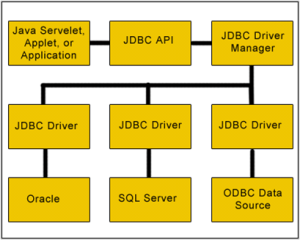
\includegraphics[width=0.70\textwidth]{figures/DA.png}}
	\caption{Arsitektur}
	\label{DA.png}
\end{figure}

 
\chapter{Sending Email}
\section {Server Pada Mail Server dan Penjelasannya} 
Pada mail server terdapat 2 server yang berbeda yaitu :  
\begin{enumerate}
\item Outgoing Server (Sending email) : Protocol server yang menangani adalah SMTP (Simple Mail Transfer Protocol) pada port 25. 
\item Incoming Server (Receiving email) : Protocol server yang menangani adalah POP3 (Post Office Protocol) pada port 110 atau IMAP (Internet Message Access Protocol) pada port 143.
 \end{enumerate}
Penjelasan dari Server yang menangani outgoing email dan incoming email sebagai berikut 
\begin{enumerate}
\item SMTP Server : Saat anda mengirimkan email maka email anda akan ditangani SMTP Server dan akan dikirim ke SMTP Server tujuan, baik secara langsung maupun melalui beberapa SMTP Server dijalurnya. Apabila server tujuan terkoneksi maka email akan dikirim, namun apabila tidak terjadi koneksi maka akan dimasukan ke dalam queue dan di resend setiap 15 menit, apabila dalam 5 hari tidak ada perubahan maka akan diberikan undeliver notice ke inbox pengirim. 
\item POP3 Server : Jika menggunakan POP3 Server, apabila kita akan membaca email maka email pada server di download sehingga email hanya akan ada pada mesin yang mendownload email tersebut (kita hanya bisa membaca email tersebut pada device yang mendownload email tersebut). 
\item IMAP Server : Jika menggunakan IMAP Server, email dapat dibuka kembali lewat device yang berbeda. Fungsinya adalah mengelola email yang disimpan di server, kemudian email tersebut di ambil oleh client, selain itu IMAP juga meneruskan packet data. Kemampuan ini jauh lebih baik daripada POP (Post Office Protocol) yang hanya memperbolehkan kita mengambil/download semua pesan yang ada tanpa kecuali. IMAP adalah suatu  protokol yang umum digunakan untuk pengiriman surat elektronik atau email di Internet. Protokol ini gunakan untuk mengirimkan data dari komputer pengirim surat elektronik ke server surat elektronik penerima. Untuk menggunakan SMTP bisa dari Microsoft Outlook. biasanya untuk menggunakan SMTP di perlukan settingan :
\end{enumerate} 
\begin{itemize}
\item Email Address : contoh; 
\begin{enumerate}
\item anda@domainanda.com 
\item Incoming Mail (POP3, IMAP or HTTP) server : mail.domainanda.com 
\item Outgoing (SMTP) server : mail.domainanda.com 
\item Account Name : anda@domainanda.com 
\item Password : password yang telah anda buat sebelumnya
\end{enumerate} 
\end{itemize}
Pada ilustrasi diatas Siti memiliki alamat email siti@a.id menulis email nya di komputer menggunakan Thunderbird atau Evolution. Pada kolom To: dia ketikkan alamat tujuan yaitu hendra@b.id. Setelah siti menekan tombol send, email yang dikirim langsung menuju ke mesin SMTP server milik ISP 1 yang bernama smtp.a.id
Pada server smtp.a.id menerima email dari siti (siti@a.id) yang ditujukan kepada hendra (hendra@b.id). Server mengecek smtp.a.id mencek alamat email tujuan yaitu hendra.@b.id. Mesin server smtp.a.id membutuhkan informasi ke server mana email untuk mesin.b.id harus ditujukan. Untuk memperoleh informasi tersebut tentang domain b.id. 
Kemudian pada mesin Name Server ns.b.id memberitahukan mesin smtp.a.id bahwa semua email yang ditujukan kepada b.id harus dikirim kepada mesin smtp.b.id.Setelah memperoleh jawaban dari ns.c.id bahwa email harus dikirm ke mesin smtp.b.id maka mesin smtp.a.id berusaha untuk menghubungi mesin smtp.b.id.Setelah mesin smtp.b.id berhasil dihubungi, mesin smtp.a.id mengirimkan teks email dari Siti (siti@a.id) yang ditujukan kepada Hendra(henra@b.id) ke mesin smtp.b.id 
Hendra (hendra@b.id)yang sedang menjalankan perangkat lunak pembaca email dan mengambil email tersebut dari eail server smtp.b.id barulah email dari Siti (siti@a.id) dapat diunduh melalui PC hendra dan di tampilkan isi emailnya. 
E-mail disampaikan oleh mail client (MUA, mail user agent) ke mail server (MSA, mail submission agent) menggunakan SMTP pada port 587 atau menggunakan traditional port 25. Dari sini, MSA mengirim mail tersebut ke mail transfer agent miliknya (MTA, mail transfer agent). MTA batas harus menemukan host target, dengan menggunakan DNS untuk mencari mail exchange record (MX record) untuk domain penerima. MX record yang kembali berisi nama dari host target. MTA selanjutnya menghubungkan ke exchange server sebagai SMTP client. Ketika MX target menerima pesan yang masuk, akan ditangani oleh mail delivery agent (MDA) untuk pengiriman pesan secara local. 
Analisis: Saat PC siti diberi perintah mengirim email ke PC Hendra, kemudian email tersebut terlebih dahulu masuk ke server network dimana dia berada server 1(smtp.a.id), disini server dapat melakukan kegiatan sniffing, Pada server sebelumnya sudah saling terkoneksi dan mendapat authentifikasi dari antar server untuk meneruskan paket email yang akan dikirim protokol yang bekerja pada tahap ini adalah SMTP, kemudian email masuk pada server2 (smtp.b.id).Untuk selanjutnya email dikirim ke PC Hendra (PC Destination) pada tahap ini protokol yang bekerja adalah protokol IMAP. Sehingga dari ilustrasi yang diberikan dapat menggambarkan proses pengiriman email,dan apa saja yang terjadidalam prosesnya. 
Pada proses pengiriman email terjadi kegiatan sniffing yang dilakukan oleh server. Sniffing adalah kegiatan pengendusan traffic data packet pada suatu jaringan. 
Selain itu Prinsip kerja dan Porses Pengiriman Email, email juga dibedakan berdasarkan format isinya, yakni sebagai berikut
\begin{itemize} 
\item Plain Text Email adalah jenis email yang sisanya diformat menggunakan sistem America Standart Code for Information Interchange (ASCII). Tulisan yang dibuat dengan format ini tidak dapat dimodifikasi seperti warna, ukuran jenis font dan lain sebagainya, Tidak ada pengolahan atau penambahan aksesoris. 
\item HTML Email adalah bahasa standar yang digunakan untuk mengatur tampilan informasi di Internet. Email yang menggunakan format ini umumnya dapat disesuaikan dengan selera pengirimnya, Dengan begitu email tersebut dapat ditambahkan macam-macam aksesoris seperti; penggantian jenis font, warna font dan juga besaran font pada tiap bagian surat.
\end{itemize}
\subsection {Apa Itu Port ?} 
Port adalah socket atau jack koneksi yang terletak di luar unit sistem sebagai tempat kabel - kabel yang berbeda ditancapkan. Port berfungsi untuk mentransmisikan data. Berikut macam - macam port : 
\begin{enumerate}
\item Port Serial adalah port seri merupakan sebuah port pada personal computer yang berfungsi untuk mentransmisikan satu bit informasi pada satu satuan waktu. 
\item Port Pararel adalah sebuah port pada personal computer yang berfungsi sebagai alat komunikasi komputer (motherboard) dengan perangkat luar yang bersifat paralel. 
\item Port SCSI (Scuzzy) adalah port berkinerja tinggi yang didefinisikan oleh American National Standart Institute yang digunakan untuk menangani perangkat input/output atau perangkat media penyimpanan. 
\item Port USB adalah suatu teknologi yang memungkinkan untuk menghubungkan alat eksternal (peripheral) seperti scenner, printer, mouse, dan perangkat lainnya ke komputer. \par
\end{enumerate}
\subsection {Cara Kerja Mail Server (singkat)} 
Cara kerja mail server mempunyai berbagai macam versi penjelasan mengenai cara kerjanya, dalam artikel ini saya akan menjelaskan 2 versi cara kerja mail server yang sudah saya rangkum dari berbagai sumber. Sebenarnya cara kerja antara versi 1 dan 2 mempunyai inti yang sama, hanya saja penjelasannya yang beda, silahkan anda pilih yang mana.\par  
\begin{itemize}
\item Cara Kerja Mail Server Versi 1 :
Proses pengiriman e-mail malalui tahapan yang sedikit panjang. Saat e-mail di kirim, maka e-mail tersebut disimpan pada mail server menjadi satu file berdasarkan tujuan e-mail. File ini berisi informasi sumber dan tujuan, serta dilengkapi tanggal dan waktu pengiriman. Pada saat user membaca e-mail berarti user telah mengakses server e-mail dan membaca file yang tersimpan dalam server yang di tampilkan melalui browser user 
\item Cara Kerja Mail Server Versi 2:
Cara kerja ini saya ambil dari Xmodulo, sebelum memahami proses cara kerja mail server sebaiknya anda mengenal terlebih dahulu singkatan - singkatan dari MUA, MTA, MDA dll. Berikut penjelasannya : 
\begin{enumerate}
\item Mail User Agent (MUA) : MUA adalah komponen yang berinteraksi dengan pengguna akhir secara langsung. Contoh dari MUA yaitu Thunderbird, MS Outlook, Zimbra Desktop. Interface webmail seperti Gmail. 
\item Mail Transfer Agent (MTA) : MTA bertanggung jawab untuk mentransfer email dari mail server mengirimkan sampai ke server penerima email. Contoh MTA yaitu sendmail dan postfix 
\item Mail Delivery Agent (MDA) : Dalam surat server tujuan, MTA lokal menerima email masuk dari MTA yang paling jauh. Email tersebut kemudian dikirimkan ke kotak surat pengguna dengan MDA. 
\item POP / IMAP : POP dan IMAP adalah protokol yang digunakan untuk mengambil email dari kotak surat penerima server untuk penerima MUA. 
\item Mail Exchanger Record (MX) : Record MX adalah entri DNS untuk mail server. Catatan ini menunjuk ke alamat IP ke arah mana email harus ditembak. MX record terendah selalu menang, yaitu mendapat prioritas tertinggi. Sebagai contoh, MX 10 adalah lebih baik daripada MX 20, alamat IP dari MX record dapat bervariasi berdasarkan desain dan konfigurasi persyaratan. seperti yang akan dibahas nanti dalam artikel.
Ketika pengirim mengklik tombol kirim, SMTP (MTA) memastikan ujung ke ujung pengiriman email dari pengirim-sisi server ke server tujuan. Setelah mencapai server tujuan, MTA lokal ke server tujuan menerima email, dan di pindahkan ke MDA setempat. MDA kemudian menulis email ke kotak pesan penerima. Ketika penerima memeriksa email, mereka diambil oleh MUA dengan menggunakan protokol seperti POP atau IMAP. 
\end{enumerate}
\end{itemize}

\section{Sending Email}
	Mail Server adalah perangkat lunak program yang mendistribusikan file atau informasi sebagai respons atas permintaan yang dikirim via email, mail server juga digunakanpadabitnetuntukmenyediakanlayananserupaftp. Selainitumailserverjuga dapat dikatakan sebagai aplikasi yang digunakan untuk penginstalan email.	\par \vspace{12pt}
	Tak hanya sebagai sebuah program mail server juga bisa berupa sebuah komputer yang memang dikhususkan untuk menjalankan sebuah aplikasi perangkat lunak program ini. nah komputer ini di ibaratkan sebagai jantung dari system sebuah email. Program ini biasanya dikelola oleh programer yang disebut dengan post master.	\par \vspace{12pt}
	Mail server ini dikelola oleh seorang post master yang memiliki beberapa tugas pokok yaitu mengelola kaun, memonitor bagaimana kinerja server dan melaksanakan tugas administrative lainnya. Biasanya program ini menggunakan protocol antara lain smtp, pop3 dan imap.	\par \vspace{12pt}
	
	\textbf{Cara Kerja Mail Server}	\par \vspace{12pt}
	
	Setelah kamu tahu apa itu mail server, kini saatnya kamu tahu bagaimana mail server bekerja. Pada dasarnya ada dua cara kerja program ini. pertama, proses pengiriman email akan melewati tahapan yang agak panjang. saat email dikirim karena email akan disimpan pada server utama atau email server itu sendiri berdasarkan tujuan email akan dikirimkan kemana. Umumnya file ini berisi informasi yang dimana sumber tujuan, serta adanya waktu pengiriman. Nah saat kamu sebagai user membaca email berarti user telah mengakses server email tersebut dan membaca email yang tersimpan pada server yang di tampilkan pada browser pengguna.	\par \vspace{12pt}
	
	Untuk memahami cara kerja mail server yang kedua ini,kamu harus memahami ada beberapa istilah penting yaitu MUA atau mail user agent yaitu sebuah komponen yang berinteraksi secara langsung, misalnya adalah thunderbird, ms outlook, zimbra atau interface webmail seperti gmail ataupun yahoo.	\par \vspace{12pt}
	
	Selain itu istilah penting mail server lainnya adalah MTA atau mail transfer agent yang bertanggung jawab mentransfer email dari server mail kemudian sampai server mail penerima, contohnya adalah karena sendmail dan postfix. Selain itu MDA atau mail delivery agent, jika mta lokasi menerima email masuk dari mta terpencil maka email akan dikirim kek otak pengguna dengan mda.	\par \vspace{12pt}
	
	Istilah lain dalam mail server ada POP atau IMAP kedua singkatan ini merupakan sesuatu protocol yang digunakan untuk mengunduh email dari kotak penerima server untuk penerima MUA. Kemudian ada mail exchange record atau MX. Istilah ini merujuk pada entri dns untuk server mail. Record mx ini akan menunjuk pada alamt ip dimana email harus ditembakkan. Mx record yang rendah akan selalu menang karena mendapat priritas tertinggi. Contohnya misal mx 10 akan lebih baik dibandingkan dengan mx 20.	\par \vspace{12pt}
	
	Mail Server juga bisa disebut sebagai sebuah komputer yang didedikasikan untuk menjalankan jenis aplikasi perangkat lunak komputer, hal ini dianggap sebagai bagian terpenting dari setiap email sistem. Mail Server biasanya dikelola oleh seorang yang biasanya dipanggil post master.
 
	Tugas Post Master:
	\begin{itemize}
		\item Mengelola Account  
		\item Memonitor Kinerja Server 
		\item Tugas Administratif Lainnya
	\end{itemize}

\subsection {Protokol Pada Mail Server}
	Protokol yang umum digunakan antara lain protokol SMTP, POP3 dan IMAP.
	
	\begin{enumerate}
		\item  SMTP (Simple Mail Transfer Protocol) 
		 	Protokol ini digunakan untuk mengirimkan data dari komputer pengirim surat elektronik ke server surat elektronik penerima. Protokol ini timbul karena desain sistem surat elektronik yang mengharuskan adanya server surat elektronik yang menampung sementara, sampai surat elektronik diambil oleh penerima yang berhak.
		 	\par \vspace{12pt}
		 	
		 	SMTP bisa kita katakan sebagai Sebuah Kantor pos, yang pada dasarnya jika kita mengirim sebuah surat pastinya Surat itu akan dibawa Ke Gudang kantor pos untuk di lakukan penyortiran, Gudang inilah yang dimaksud dengan SMTP, Setelah dilakukan penyortiran maka surat siap untuk diantarkan ketujuan, tapi tidak proses tidak berhenti disini, Jadi surat ini akan dibawa oleh si kurir lalu si Kurir Meletakkanya di Kotak Pos yang biasa kita katakan sebagai PO BOX (PO BOX inilah yang dimaksud dengan POP3) itulah penjelasan singkat tentang SMTP.
		 	\par \vspace{12pt}
		 	
		 	SMTP adalah protokol yang cukup sederhana, berbasis teks dimana protokol ini menyebutkan satu atau lebih penerima email untuk kemudian diverifikasi. Jika penerima email valid, maka email akan segera dikirim. SMTP menggunakan port 25 dan dapat dihubungi melalui program telnet. Agar dapat menggunakan SMTP server lewat nama domain, maka record DNS (Domain Name Server) pada bagian MX (Mail Exchange) digunakan.
		 	\par \vspace{12pt}
		 	
		 	SMTP (Simple Mail Transfer Protocol) digunakan sebagai standar untuk menampung dan mendistribusikan email. Simple Mail Transfer Protocol atau SMTP digunakan untuk berkomunikasi dengan server guna mengirimkan email dari lokal email ke server, sebelum akhirnya dikirimkan ke server email penerima. Proses ini dikontrol dengan Mail Transfer Agent (MTA) yang ada dalam server email Anda. Port SMTP Default:
			   
			\begin{itemize}
				\item Port~25 –  Port tanpa dienkripsi
				\item Port 426 – Port SSL/TLS, nama lainnya SMTPS
			\end{itemize}

		\item {POP3 Post Office Protocol v3}
			POP3 (Post Office Protocol v3) dan IMAP (Internet Mail Application Protocol) digunakan agar user dapat mengambil dan membaca email secara remote yaitu tidak perlu login ke dalam sistem shelll mesin mail server tetapi cukup menguhubungi port tertentu dengan mail client yang mengimplementasikan protocol POP3 dan IMAP.
			POP3 (Post Office Protocol 3) adalah versi terbaru dari protokol standar untuk menerima email. POP3 merupakan protokol client/server dimana email dikirimkan dari server ke email lokal. Digunakan untuk berkomunikasi dengan email server dan mengunduh semua email ke email lokal (seperti Outlook, Thunderbird, Windows Mail, Mac Mail, dan sebagainya), tanpa menyimpan salinannya di server. Biasanya, dalam aplikasi email terdapat pilihan untuk tetap menyimpan salinan email yang diunduh pada server atau tidak.

			Apabila kita mengakses akun email yang sama dari perangkat berbeda, akan sangat direkomendasikan untuk menyimpan backup. Hal ini perlu dilakukan sebagai langkah antisipasi apabila perangkat kedua tidak bisa mengunduh email, sementara perangkat pertama sudah menghapusnya.\par \vspace{12pt} 

			POP3 adalah sebuah protocol internet yang digunakan untuk mengakses email atau surat elektronik yang masuk ke dalam email client. Fungsi utama dari POP3 ini adalah untuk menyimpan sementara email yang terkirim di dalam sebuah email server, dan kemudian meneruskannya ke dalam email client, dimana baru akan terespon ketika email tersebut sudah dibuka oleh user yang berhak (dalam hal ni adalah mereka yang memegang username dan juga password dari alamat email).
			\par \vspace{12pt}
			
			POP3 adalah protokol komunikasi satu arah, yang artinya data diambil dari server dan dikirimkan ke email lokal di perangkat komputer Anda. 
Port POP3 Default:
			\begin{itemize}
			\item Port 110 Port tanpa dienkripsi
			\item Port 995 Port SSL/TLS, nama lainnya POP3S
			\end{itemize}
	\end{enumerate}

\subsubsection {Kelebihan Menggunakan POP3}
	\begin{enumerate}
		\item Ketika email sudah diunduh melalui aplikasi local mail di komputer, Anda tidak perlu terhubung ke internet apabila Anda ingin membukanya kembali. 
		\item Kebanyakan tidak ada ukuran limit untuk email yang dikirim dan diterima. 
		\item Dapat membuka file attachment dengan cepat.
		\item Tidak ada ukuran maksimal untuk mailbox, kecuali harddisk komputer Anda penuh.
	\end{enumerate}
	
\subsection {Kekurangan Menggunakan POP3} 
	\begin{enumerate}
		\item Jika JavaScript pada email reader diaktifkan, email phishing dengan embed JavaScript dapat terbaca di email. 
		\item Semua pesan akan disimpan di komputer. Hal ini dapat mengurangi space pada harddisk komputer.
		\item Semua file attachment diunduh dan disimpan dalam komputer. Karenanya, potensi komputer terinfeksi virus dari email lebih besar. \item Folder email terkadang hilang. Jika ini yang terjadi, upaya restore cukup sulit dilakukan.
	\end{enumerate}

\subsection {IMAP (Internet Message Access Protocol)}
	 IMAP (Internet Message Access Protocol) adalah protokol standar untuk mengakses/mengambil e-mail dari server. IMAP memungkinkan pengguna memilih pesan e-mail yang akan ia ambil, membuat folder di server, mencari pesan e-mail tertentu, bahkan menghapus pesan e-mail yang ada. Kemampuan ini jauh lebih baik daripada POP (Post Office Protocol) yang hanya memperbolehkan kita mengambil/download semua pesan yang ada tanpa kecuali.\par \vspace{12pt}
	Internet Message Access Protocol merupakan salah satu dari dua protokol penerimaan email (email retrieval protocol). Juga dikenal dengan singkatan IMAP, Internet Message Access Protocol merupakan Internet protocol yang beroperasi pada Application layer. Dengan IMAP, mailbox dapat dibaca dan dikelola secara simultan (bersamaan) oleh sejumlah email client berbeda. IMAP seringkali digunakan oleh sebagian besar pengguna Internet untuk mendownload email dari web mail server.\par \vspace{12pt}
	Awalnya disebut sebagai Interim Mail Access Protocol, versi IMAP pertama telah menjalani beberapa revisi sejak dibuat pada tahun 1986. Saat ini disebut sebagai Internet Message Access Protocol, versi IMAP ini merupakan versi IMAP keempat yang telah menjadi standar pada tahun 1994, dan dipublikasikan pada RFC 1730. Pop Office Protocol (POP) merupakan Internet protocol umum lainnya untuk email retrieval. Sebagian besar email server dan email client mendukung baik IMAP dan POP sebagai pilihan lain terhadap protokol unik mereka sendiri. Dibandingkan dengan POP, IMAP memiliki beberapa keunggulan termasuk kemampuan untuk memuat bagian dari email ketimbang menunggu semua attachment di dalamnya. IMAP juga dapat juga menerima konten pesan menggunakan mekanisme MIME. IMAP client juga cenderung tetap dapat terhubung dengan mail server dalam periode waktu yang lebih lama, yang dapat meningkatkan response time secara keseluruhan. \par \vspace{12pt}
	 Cara kerja IMAP adalah email client melakukan koneksi ke server email, lalu melakukan sinkronisasi folder. Apabila kita mengklik/ mengakses sebuah folder, maka daftar email berikut isinya (?) juga didownload. Apabila kita menghapus sebuah email, maka email pada server juga dihapus. Dengan kata lain, protokol IMAP seakan-akan memindahkan semua isi mailbox kita ke e-mail clent kita sendiri.\par \vspace{12pt}
	Pada dasranya Protokol IMAP ini dirancang agar user dapat mengakses e-mail pada milbox serta dapat berinteraksi dengan server. PORT yang digunakan untuk protocol ini dalam bentuk TCP/IP yaitu pada PORT nomer 143. Protocol ini menggunakan koneksi yang terus menerus ke server. Ketika e-mail masuk maka anda akan melihat langsung di e-mail kmputer Client (dengan posisi online). Karena e-mail yang masuk ke server maka akan cepat masuk dan dapat segera dilihat juga di Client. Seringkali lebih cepat prosesnya dibandingkan jika menggunakan web interface sendiri yang mirip seperti Blackberry. Namun untuk menggunakan IMAP anda harus menggunakan Koneksi Internet yang cukup baik atau dengan bandwidth yang lumayan besar. Bahkan dengan IMAP jika anda menggunakan 10 client interface web, missal menggunakan Netbook,Notbook,Dekstop, Ponsel danlain sebagainya maka semua akan memperlihatkan e-mail yang sama. Jika anda menggunakan banyak device untuk mengakses e-mail, maka pilihan yang tepat adalah menggunakan IMAP. Karena IMAP lebih baik dengan POP. Tapi IMAP biasanya digunakan untuk dalam jaringan LAN saja karena untuk kapasitas jaringan kecil akan lebih maksimal, jika untuk kapasitas yang lebih besar lagi pilihan yang tepat adalah menggunakan Protokol POP3.\par \vspace{12pt}
	IMAP (Internet Message Access Protocol), seperti halnya POP3, juga digunakan untuk mengirimkan email ke local mail, hanya saja terdapat sedikit perbedaan cara kerja.
	IMAP merupakan protokol komunikasi dua arah sebagai perubahan yang dibuat pada local mail yang dikirimkan ke server. Pada dasarnya, isi email tetap berada di server. Protokol IMAP lebih direkomendasikan oleh penyedia email seperti Gmail dibandingkan menggunakan POP3.
	Dalam IMAP, email disimpan di server. ketika Anda akan mengecek email, local mail akan menghubungi server untuk menampilkan pesan email. Sehingga untuk file pesan email tetap berada di server dan tidak didownload ke email lokal. Port IMAP Default: 
	\begin{enumerate}
		\item Port 143 – Port tanpa dienkripsi 
		\item Port 993 – Port SSL/TLS, nama lainnya IMAPS
	\end{enumerate}

\subsection {Menggunakan SMTP pada python}
Python memiliki sebuah modul bernama SMTP Server yang dapat digunakan untuk menerima e-mail dari client dan menampilkan isinya ke stdout alias konsol. 
	contoh client yang mengirim e-mail ke SMTP server ini:
	\begin {verbatim}
		import smtplib
		sender = 'mikail@website.com'
		recipient = ['sonanjaya@website.com']

		message = """From: From Person <%s>
		To: To Person <%s>
		Subject: Testing SMTP E-Mail

		Pesan ini dikirim melalui smtplib dan diterima oleh modul SMTP Server Python.

		""" % (sender, recipient)

		try:

   		smtpObj = smtplib.SMTP('localhost', 1025)
   		smtpObj.sendmail(sender, recipient, message)    

   		print "Mengirim e-mail berhasil :D..."

		except Exception, e:

		print str(e)
   		print "Error: e-mail gagal terkirim :(..."
	\end{verbatim}

Pada kode diatas dengan menggunakan smtplib cukup dengan mengakses URL dan port yang dituju, lalu kirim e-mail dengan menggunakan method sendmail() dengan melewatkan pengirim, penerima, dan pesan.

\begin{table}[ht]
	\caption{Contoh email yahoo yang memiliki smtp}
	\centering
	\begin{tabular}{cccc}
		\hline
		No&Keterangani&\\
		\hline
		.1&Yahoo POP Server - pop.mail.yahoo.com port-995&\\
		.2&Requires SSL-Yes&\\
		\hline
	\end{tabular}
\end{table}

\ref{smtp.png}:
\begin{figure}[ht]
	\centerline{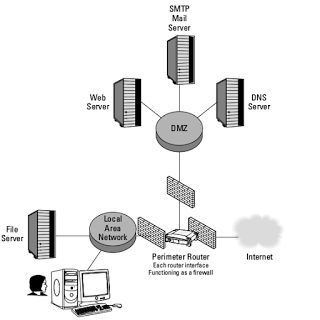
\includegraphics[width=0.70\textwidth]{figures/smtp.png}}
	\caption{SMTP}
	\label{smtp.png}
\end{figure}

\textbf{Skema Singkat}\par \vspace{12pt}
Mail Server atau yang sering disebut juga E-Mail server, digunakan untuk mengirim surat melalui Internet. Dengan begitu, dapat mempermudah dalam penggunanya, karena lebih cepat dan efisien. Untuk membuat Mail Server, harus terdapat SMTP dan POP3 server, yang digunakan untuk mengirim dan menerima email. Proses pengiriman email bisa terjadi karena adanya SMTP Server (Simple Mail Transfer Protocol). Setelah dikirim, email tersebut akan ditampung sementara di POP3 Server (Post Office Protocol ver. 3). Dan ketika user yang mempunyai email account tersebut online, mail client akan secara otomatis melakukan sinkronisasi dari POP3 Server.
\par \vspace{12pt}
Mungkin kita dulu pernah bahkan sering menggunakan kantor pos sebagai jasa untuk mengirim surat kepada kerabat atau teman kita yang jauh dari tempat kita tinggal, di Kantor pos itu juga terdapat Kurir sebagai tukang mengantarkan surat dari Kantor Pos kepada penerima.
\par \vspace{12pt}
SMTP ini singkatan dengan kepanjangan Simple Mail Transfer Protocol. Dengan pengertian singkat SMTP adalah protokol yang mengatur pengiriman email dari pengirim (Ongoing).
Cara kerja SMTP ini sama dengan Kantor Pos, tempat dimana kita menitipkan surat kita agar dikirimkan kepada penerima yang tertera di surat tersebut.
Terdapat pada port berapa SMTP? SMTP terdapat pada port 25.
\par \vspace{12pt}
POP3 ini singkatan dari kepanjangan Post Office Protocol ver.3 dan IMAP ini singkatan dari kepanjangan Internet Message Access Protocol. Dengan pengertian singkat POP3/IMAP adalah protokol yang mengatur penerimaan email kepada penerima (Ingoing).\par \vspace{12pt}
Cara kerja POP3 dan IMAP sama dengan kurir yang mengantarkan surat, tugasnya menyampaikan surat yang sebelumnya sudah dititipkan di Kantor Pos (SMTP) kepada penerima surat.
Terdapat pada port berapa POP3? POP3 terdapat pada port 110.
Terdapat pada port berapa IMAP? IMAP terdapat pada port 143.

Ada perbedaan antara POP3 dan IMAP, mudahnya. kalau IMAP itu protokol yang biasa kita pakai kalau kita pakai Web Based Mail, contohnya seperti (gmail.com, yahoo.com) dan menggunakan Browser sebagai antarmukanya, kalau POP3 menggunakan Aplikasi Email Client, sebut saja Outlook, Thunderbird, Outlook Express dll.

Bedanya jika kita pakai IMAP, kita hanya bisa melihat isi dari email yang ada pada mailbox kita secara online dan tidak bisa di download ke localdisk kita, berbeda dengan POP3 yang bisa membuka email secara offline dengan syarat ketika komputer online dia mendownload semua email ke local disk sehingga bisa dibaca offline.

\chapter{Multithreading}
\section{Multithreading}
\hspace*{0.5in} Menjalankan beberapa\textit{ thread} mirip dengan menjalankan beberapa program yang berbeda secara bersamaan, namun dengan manfaat berikut : \par

\begin{itemize}
\item Beberapa \textit{thread} dalam proses berbagi ruang data yang sama dengan benang induk dan karena dapat saling berbagi informasi atau berkomunikasi satu sama lain dengan lebih muda daripada jika prosesnya terpisah \par

\item \textit{thread} terkadang disebut proses ringan dan tidak membutuhkan banyak memori atas, mereka lebih murah daripada proses.\end{itemize}
\par

\vspace{12pt}
\hspace*{0.5in} Sebuah \textit{thread} memiliki permulaan, urutan eksekusi dan sebuah kesimpulan. Ini memiliki pointer perintah yang melacak dari mana dalam konteksnya saat ini berjalan. \par

\begin{itemize}
\item Hal ini dapat dilakukan sebelum pre-\textit{empted} (\textit{inturrepted})\end{itemize}
\par
\noindent 
\begin{itemize}
\item Untuk sementara dapat ditunda sementara \textit{thread} lainnya yang sedang berjalan ini disebut unggul. \end{itemize}
\par
\noindent 
\subsection{Memulai Thread Baru} \par
\noindent 
\hspace*{0.5in} Untuk melakukan \textit{thread} lain, perlu memanggil metode berikut yang tersedia dimodul \textit{thread} : \par
\noindent 
\begin{center}{\fontsize{9pt}{9pt}\selectfont Thread.start $  \_  $new $  \_  $thread (function, args [, kwargs] )}\end{center} \par
Pemanggilan metode ini memungkinkan cara cepat dan tepat untuk membuat \textit{thread} baru di linux dan window. \par
\hspace*{0.5in} Pemanggilan metode segera kembali dan anak  \textit{thread} dimulai dan fungsi pemanggilan dengan daftar \textit{args} telah berlalu. Saat fungsi kembali ujung \textit{thread} akan berakhir. Disini, \textit{args }adalah tupel argumen. Gunakan tupel kosong untuk memanggil fungsi tanpa melewati argumen. \textit{Kwargs} adalah kamus opsional argumen kata kunci.  \par

\vspace{12pt}
Contoh : 
\begin{verbatim}
\#  $!/usr/bin/python} 

Import thread
Import time

#  $ Define a function for the thread 

Def print $  \_  $time (threadNamw, delay):
Count = 0
While count <5:
Time.sleep(delay)
Count +=1 
Print  $ " $ $  \%  $s :  $  \%  $s $ " $  $  \%  $ 
(threadName, time.ctime(time.time()))

#  $ Create two thread as follows
try:
thread.start $  \_  $new $  \_  $thread(print $  \_  
$time, ( $ " $Thread-1 $ " $, 2, ))
thread.start $  \_  $new $  \_  $thread(print $  \_  
$time, ( $ " $Thread-2 $ " $, 4,))
except: 
print " $Error: unable to start thread 

while 1:
pass 
\end{verbatim}

\vspace{80pt}	
Bila kode diatas dieksekusi, maka menghasilkan hasil sebagai berikut : \par
\vspace{10pt}
\noindent 
\begin{center}{\fontsize{10pt}{10pt}\selectfont Thread-1 : Thu Jan 22 15:42:17 2009}\end{center} \par
\noindent 
\begin{center}{\fontsize{10pt}{10pt}\selectfont Thread-1 : Thu Jan 22 15:42:19 2009}\end{center} \par
\noindent 
\begin{center}{\fontsize{10pt}{10pt}\selectfont Thread-2 : Thu Jan 22 15:42:19 2009}\end{center} \par
\noindent 
\begin{center}{\fontsize{10pt}{10pt}\selectfont Thread-1 : Thu Jan 22 15:42:21 2009}\end{center} \par
\noindent 
\begin{center}{\fontsize{10pt}{10pt}\selectfont Thread-2 : Thu Jan 22 15:42:23 2009}\end{center} \par
\noindent 
\begin{center}{\fontsize{10pt}{10pt}\selectfont Thread-1 : Thu Jan 22 15:42:23 2009}\end{center} \par
\noindent 
\begin{center}{\fontsize{10pt}{10pt}\selectfont Thread-1~:  Thu Jan 22 15:42:23 2009}\end{center} \par
\noindent 
\begin{center}{\fontsize{10pt}{10pt}\selectfont Thread-1 : Thu Jan 22 15:42:25 2009}\end{center} \par
\noindent 
\begin{center}{\fontsize{10pt}{10pt}\selectfont Thread-2 : Thu Jan 22 15:42:27 2009}\end{center} \par
\noindent 
\begin{center}{\fontsize{10pt}{10pt}\selectfont Thread-2 : Thu Jan 22 15:42:31 2009}\end{center} \par
\noindent 
\begin{center}{\fontsize{10pt}{10pt}\selectfont Thread-2 : Thu Jan 22 15:42:35 2009}\end{center} \par

\vspace{12pt}
\hspace*{0.5in} Meskipun sangat efektif untuk benang tingkat rendah, namun modul \textit{thread} sangat terbatas dibandingkan dengan modul yang baru. \par

\vspace{12pt}
\subsection {Modul Threading} \par
\hspace*{0.5in} Modul threading yang lebih baru disertakan dengan Python 2.4 memberikan jauh lebih kuat, dukungan tingkat tinggi untuk \textit{thread}\textit{ }dari modul\textit{ }\textit{thread}\textit{ }dibahas pada bagian sebelumnya. \par
\hspace*{0.5in} The \textit{thread}\textit{ing }modul mengekpos semua metode dari \textit{thread}\textit{ }dan menyediakan beberapa metode tambahan : \par

\begin{itemize}
\item \textbf{t}\textbf{hreading.activeCount() } \par
Mengembalikan jumlah objek \textit{thread} yang aktif \par
\item \textbf{t}\textbf{hreading.currentThread() } \par
Mengembalikan jumlah objek \textit{thread} dalam kontrol benang pemanggil \par
\item \textbf{t}\textbf{hreading.enumerate() } \par
Mengembalikan daftar semua benda \textit{thread}\textit{ }yang sedang aktif \par

\vspace{12pt}
\hspace*{0.5in} Selain metode, modul \textit{thread}\textit{ing }memiliki \textit{thread}\textit{ }kelas yang mengimplementasikan \textit{thread}\textit{ing. }Metode yang disediakan oleh \textit{thread}\textit{ }kelas adalah sebagai berikut : \par
\item \textbf{run()} \par
Metode adalah titik masuk untuk \textit{thread} \par
\item \textbf{start()} \par
Metode dimulai\textbf{ }\textit{thread}\textit{ }dengan memanggil metode run \par
\item \textbf{join(}\textbf{[time]}\textbf{)} \par
Menunggu benang untuk mengakhiri \par
\item \textbf{isAlive()} \par
Metode memeriksa apakah\textbf{ }\textit{thread}\textit{ }masih mengeksekusi\textbf{ } \par
\item \textbf{getName()} \par
Metode mengambalikan nama\textbf{ }\textit{thread} \par
\item \textbf{setName()} \par
Metode menetapkan nama\textbf{ }\textit{thread} \par

\vspace{12pt}
\subsection {Membuat Thread Menggunakan Modul} \par
\hspace*{0.5in} Untuk melaksanakan \textit{thread}\textit{ }baru menggunakan\textit{ threading} harus melakukan hal berikut : \par
\item Mendefinisikan subclass dari \textit{thread} kelas \par
\item Menimpa  $  \_  $init $  \_  $ (self [args]) metode untuk menambahkan argumen tambahan \par
\item Menimpa run(self[args]) metode untuk menerapkan apa \textit{thread} harus dilakukan ketika mulai 
\end{itemize}

\vspace{12pt}
\hspace*{0.5in} Setelah membuat baru \textit{thread} subclass, dapat membuah seuah instance dari itu dan kemudian memulai \textit{thread} baru dengan menerapkan \textit{start(),} yang ada gilirinnya panggilan \textit{run()} metode. \par
\vspace{50pt}

Contoh :
\begin{verbatim} 
#  $!/usr/bin/python

import threading
import time

exitFlag = 0

class myThread (threading.Thread): 
def $  \_  $init $  \_  $(self, threadID, name, 
counter) :
threading.Thread. $  \_  $init $  \_  $(self)} 
self.threadID = threadID
self.name = name 
self.counter = counter 
def run (self) :
print  $ " $Starting  $ " $ + self.name 
print $  \_  $time(self.name, self.counter, 5)
print  $ " $Exiting  $ " $+ self.name

def print $  \_  $time(threadName, delay, counter):} 

while counter:

if exitFlag: 
threadName.exit() 
time.sleep(delay) 
print  $ " $ $  \%  $s:  $  \%  $s $ " $  $  \%  
$ (threadName, time.ctime(time.time()))
counter -= 1} 

#  $ Create new threads
thread1 = myThread(1,  $ " $Thread-1 $ " $, 1)
thread2 = myThread(2,  $ " $Thread-2 $ " $, 2)
#  $ Start new threads
thread1.start()
thread2.start()
print  $ " $Exiting Main Thread $ " $
\end{verbatim}

\vspace{12pt}
Ketika kode diatas dijalankan, menghasilkan hasil sebagai berikut:
\par
\noindent 
{\fontsize{10pt}{10pt}\selectfont Starting Thread-1} \par
\noindent 
{\fontsize{10pt}{10pt}\selectfont Starting Thread-2} \par
\noindent 
{\fontsize{10pt}{10pt}\selectfont Exiting Main Thread} \par
\noindent 
{\fontsize{10pt}{10pt}\selectfont Thread-1 : Thu Mar 21 09:10:03 2013} \par
\noindent 
{\fontsize{10pt}{10pt}\selectfont Thread-1 : Thu Mar 21 09:10:04 2013} \par
\noindent 
{\fontsize{10pt}{10pt}\selectfont Thread-2 : Thu Mar 21 09:10:04 2013} \par
\noindent 
{\fontsize{10pt}{10pt}\selectfont Thread-1 : Thu Mar 21 09:10:05 2013} \par
\noindent 
{\fontsize{10pt}{10pt}\selectfont Thread-2 : Thu Mar 21 09:10:06 2013} \par
\noindent 
{\fontsize{10pt}{10pt}\selectfont Thread-1 : Thu Mar 21 09:10:07 2013} \par
\noindent 
{\fontsize{10pt}{10pt}\selectfont Exiting Thread-1} \par
\noindent 
{\fontsize{10pt}{10pt}\selectfont Thread-2 : Thu Mar 21 09:10:08 2013} \par
\noindent 
{\fontsize{10pt}{10pt}\selectfont Thread-2 : Thu Mar 21 09:10:10 2013} \par
\noindent 
{\fontsize{10pt}{10pt}\selectfont Thread-2 : Thu Mar 21 09:10:12 2013} \par
\noindent 
{\fontsize{10pt}{10pt}\selectfont Exiting Thread=2} \par

\vspace{10pt}
\subsection{Sinkronisasi Thread} \par
\hspace*{0.5in} \textit{T}\textit{hread}\textit{ing }modul disediakan dengan Python termasuk sederhana untuk menerapkan mekanisme bahwa memungkinkan untuk menyinkronkan \textit{thread}\textit{ }penguncian. Sebuah kunci baru dibuat dengan memanggil \textit{lock() }metode yang mengembalikan kunci baru. \par
\hspace*{0.5in} The \textit{acquire}\textit{ }\textit{(blocking)}\textit{ }metode objek kunci baru digunakan untuk memaksa \textit{thread}\textit{ }untuk menjalankan serempak. Opsional \textit{blocking} parameter memungkikan untuk mengontrol apakah\textit{ thread} menunggu untuk mendapatkan kunci. \par
\hspace*{0.5in} Jika \textit{blocking} diatur ke 0, \textit{thread} segera kembali dengan nilai 0 jika kunci tidak dapat diperoleh dan dengan 1 jika kunci dikuisisi. Jika pemblokiran diatur ke 1, blok dan menunggu kunci yang akan dirilis. \par
\hspace*{0.5in}The \textit{release()} metode objek kunci baru digunakan untuk melepaskan kunci ketika tidak lagi diperlukan.  \par
\noindent 

\vspace{12pt}
Contoh: 
\begin{verbatim}
#  $!/usr/bin/python

import threading
import time

class myThread (threading.Thread): 
def $  \_  $init $  \_  $(self, threadID, name, 
counter):
threading.Thread. $  \_  $init $  \_  $(self)
self.threadID = threadID
self.name = name
self.counter = counter
def run(self) 
print  $ " $Starting  $ " $+ self.name 
$  \#  $ Get lock to synchronize threads 
ThreadLock.acquire() 
print $  \_  $time(self.name, self.counter, 3) 
#  $ Free lock to realease next thread
ThreadLock.release()
Def print $  \_  $time(threadName, delay, counter):
while counter:
time.sleep(delay)
print  $ " $ $  \%  $s:  $  \%  $s $ " $  $  \%  $ 
(threadName, time.ctime(time.time()))
counter -= 1
threadLock = threading.Lock() 
threads = []
#  $ Create new threads
thread1 = myThread(1,  $ " $Thread-1,1 ) 
thread2 = myThread(2,  $ " $Thread-2,2 )
#  $ Start new Threads} 
thread1.start() 
thread2.start()

#Add threads to thread list} 
threads.append(thread1)} 
thread2.append(thread2)} 
\vspace{10pt}

#  $ Wait for all threads to complete}  
Fort t in threads:
t.join()
print  $ " $Exiting Main thread $ " $
\end{verbatim}

\vspace{8pt}
Bila kode diatas dieksekusi, maka menghasilkan sebagai berikut : \par
{\fontsize{10pt}{10pt}\selectfont Starting Thread-1} \par
\noindent 
{\fontsize{10pt}{10pt}\selectfont Starting Thread-2} \par
\noindent 
{\fontsize{10pt}{10pt}\selectfont Thread-1: Thu Mar 21 09:11:28 2013} \par
\noindent 
{\fontsize{10pt}{10pt}\selectfont Thread-1: Thu Mar 21 09:11:29 2013} \par
\noindent 
{\fontsize{10pt}{10pt}\selectfont Thread-1: Thu Mar 21 09:11:30 2013} \par
\noindent 
{\fontsize{10pt}{10pt}\selectfont Thread-2: Thu Mar 21 09:11:32 2013} \par
\noindent 
{\fontsize{10pt}{10pt}\selectfont Thread-2: Thu Mar 21 09:11:34 2013} \par
\noindent 
{\fontsize{10pt}{10pt}\selectfont Thread-2: Thu Mar 21 09:11:36 2013} \par
\noindent 
{\fontsize{10pt}{10pt}\selectfont Exiting Main Thread} \par

\vspace{8pt}
\subsection{Multithreaded Antrian Prioritas} \par
\hspace*{0.5in} The queue modul memungkinkan untuk membuat objek antrian baru yang dapat menampung jumlah tertentu item. Ada metode berikut untuk mengontrol antrian : \par
\vspace{15pt}
\begin{itemize}
	\item \textbf{get()} \par
		Menghapus dan mengembalikan item dari antrian
	\par
	\item \textbf{put()} \par
		Menambahkan item ke antrian
	\par
	\item \textbf{qsize()} \par
		Mengembalikan jumlah item yang saat ini dalam antrian
	\par
	\item \textbf{empty()} \par
		Mengembalikan benar jika antrian kosong jika tidak, salah
	\par
	\item \textbf{full()}\end{itemize}
\par
	Mengembalikan benar jika antrian penuh jika tidak, salah

\vspace{12pt}
Contoh:  
\begin{verbatim}
#  $!/usr/bin/python}  

import Queue
import threading
import time

exitFlag = 0 

class myThread (threading.Thread): 
def   $  \_  $init $  \_  $(self, threadID, name, q):
threading.Thread. $  \_  $init $  \_  $(self) 
self.name = name
self.q = q
def run(self):
print  $ " $Starting  $ " $+ self.name
process $  \_  $data(self.name, self.q) 
print  $ " $Exiting  $ " $+ self.name 
def process $  \_  $data(threadName, q):
while not exitFlag:
queuLock.acquire()
if not workQueu.empty(): 
data = q.get() 
queueLock.release() 
print  $ " $ $  \%  $s processing  $  \%  $s $ " $ 
$  \%  $ (threadName, data) 
else: 
queueLock.release()
time.sleep(1) 

threadList = [ $ " $Thread-1 $ " $,  $ " $Thread-2 $
" $,  $ " $Thread-3 $ " $]
nameList = [ $ " $One $ " $,  $ " $Two $ " $,  $ "
$Three $ " $,  $ " $Four $ " $,  $ " $Five $ " $]
queueLock = threading.Lock()
workLock = Queue.Queue(10)
threads = [] 
threadID = 1 

#  $ Create new threads
For tName in threadList: 
thread = myThread(threadID, tName, workQueue)
thread.start()
thread.append(thread)
threadID +=1

#  $ Fill the queue 
queueLock.acquire() 
for word in nameList:
workQueue.put(word) 
queueLock.release()

#  $ Wait for queue to empty
while not workQueue.empty(): 
pass 

#  $ Notify threads it?s time to exit
exitFlag = 1

#  $ Wait for all threads to complete
For t in threads:
t.join()
print  $ " $Exiting Main Thread $ " $
\end{verbatim}

\vspace{10pt} 
Bila kode diatas dieksekusi, maka menghasilkan hasil sebagai berikut: \par
\vspace{12pt}
\noindent 
{\fontsize{10pt}{10pt}\selectfont Starting Thread-1} \par
\noindent 
{\fontsize{10pt}{10pt}\selectfont Starting Thread-2} \par
\noindent 
{\fontsize{10pt}{10pt}\selectfont Starting Thread-3} \par
\noindent 
{\fontsize{10pt}{10pt}\selectfont Thread-1 processing One} \par
\noindent 
{\fontsize{10pt}{10pt}\selectfont Thread-2 processing Two} \par
\noindent 
{\fontsize{10pt}{10pt}\selectfont Thread-3 processing Three} \par
\noindent 
{\fontsize{10pt}{10pt}\selectfont Thread-1 processing Four} \par
\noindent 
{\fontsize{10pt}{10pt}\selectfont Thread-2 processing Five} \par
\noindent 
{\fontsize{10pt}{10pt}\selectfont Exiting Thread-3} \par
\noindent 
{\fontsize{10pt}{10pt}\selectfont Exiting Thread-1} \par
\noindent 
{\fontsize{10pt}{10pt}\selectfont Exiting Thread-2} \par
\noindent 
{\fontsize{10pt}{10pt}\selectfont Exiting Main Thread} \par

\section{Cara menggunakan Threading untuk Membuat Benang}
\hspace*{0.5in} Threading menggabungkan semua metode thread dan menampilkan beberapa metode tambahan. Terlepas dari metode di atas, threading juga menyajikan kelas Thread yang dapat dicoba untuk mengimplementasikan thread. Ini adalah varian object-oriented dari multithreading Python. Kelas <Thread> menerbitkan metode berikut :

\begin{table}[ht]
	\caption{Ukuran}
	\begin{tabular*}{\textwidth}{@{\extracolsep{\fill}}lcc}
		\hline
		Kelas&  Penjelasan Metode&\cr
		\hline
		run():&Ini adalah fungsi entry point untuk thread manapun&\cr
		start():&Metode start () memicu thread saat metode dijalankan dipanggil&\cr
		join([time]):&Metode join () memungkinkan sebuah program untuk menunggu thread untuk diakhiri&\cr
		\hline
	\end{tabular*}
	\begin{tablenotes}
	\end{tablenotes}
\end{table}

\section{Mengimplementasikan Thread menggunakan Threading}
\hspace*{0.5in} Buatlah subkelas dari kelas Thread. Timpa metode (self [, args]) untuk memberi argumen sesuai persyaratan. Selanjutnya, timpa metode run (self [args]) untuk mengkodekan logika bisnis benang.

\hspace*{0.5in} Setelah mendefinisikan subclass Thread baru, harus memberi instantiate untuk memulai thread baru. Berikut \ref{Mengimplementasikan Thread menggunakan Threading} Mengimplementasikan Thread menggunakan Threading :
\begin{figure}[ht]
	\centerline{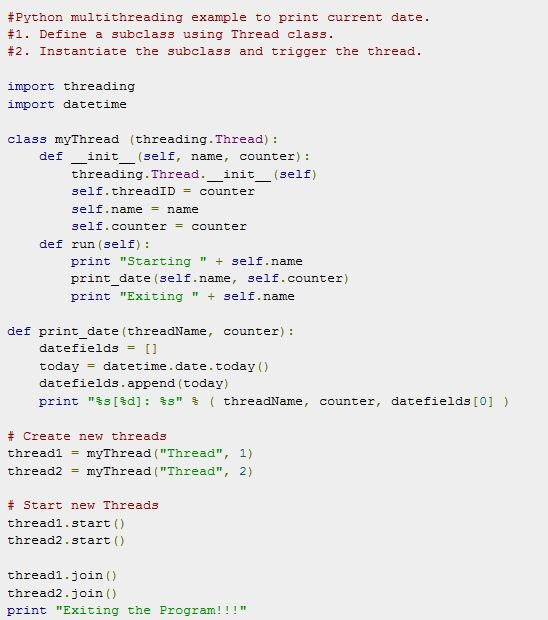
\includegraphics[width=0.75\textwidth]{figures/Thread}}
	\caption{Mengimplementasikan Thread menggunakan Threading}
	\label{Mengimplementasikan Thread menggunakan Threading}
\end{figure}


\chapter{XML Processing}

% Kelas D4 TI 3B Kelompok 3 tugas ke-3
% Diana Satima Gistivani 1154018
% M. Amran Hakim Siregar 1154106
% Indah Rahmawati 1154070
% Rizky Abdul Ghani Suherli 1154058
% Ajrina Darman 1154079

\section{XML Processing} 
\hspace*{0.5in} XML adalah bahasa open source portable yang mungkinkan pemrogram mengemangkan aplikasi yang dapat dibaca oleh aplikasi lain, terlepas dari sistem operasi dan bahasa pengembangnya. 
\vspace{12pt}
 
\hspace*{0.5in} Extensible Markup Languange (XML) adalah bahasa markup seperti HTML atau SGML. Ini direkomendasikan oleh World Wide Web Consortium dan tersedia sebagai standar terbuka. XML sangat berguna untuk mencatat data berukuran kecil dan menengah tanpa memerlukan tulang punggung berbasis SQL. 

\vspace{12pt}
\subsection{Arsitektur Parsing XML dan API} 
 
\hspace*{0.5in} Perpustakaan standar Python menyediakan seperangkat antarmuka minimal tapi berguna untuk bekerja dengan XML.  
 
\hspace*{0.5in} Dua API yang paling dasar dan umum digunakan untuk data XML adalah antarmuka SAX dan DOM. 
 
\hspace*{0.5in} API sederhana untuk XML (SAX): mendaftarkan panggilan kemali untuk acara yang diminati dan kemudian membiarkan parser berjalan melalui dokumen. Ini berguna bila dokumen berukuran besar atau memiliki keterbatasan memori, ini memparsing file tidak pernah tersimpan dalam memori. 
 
\hspace*{0.5in} API Document Objek Model (DOM): ini adalah rekomendasi World Wide Web Consortium dimana keseluruhan file dibaca ke memori dan disimpan dalam bentuk hierarkies (tree-based) untuk mewakili semua fitur dokumen XML.  
 
\hspace*{0.5in} SAX jelas tidak bisa memproses informasi secepat DOM saat bisa bekerjadengan file besar. Di sisi lain, menggunakan DOM secara eklusifenar-benar dapat membunuh sumber daya, terutama jika digunakan pada banyak file kecil. 
 
\hspace*{0.5in} SAX hanya bisa dibaca sementara DOM mengizinkan perubahan pada file XML. Kedua API yang berbeda ini saling melengkapi satu sama lain, tidak ada alasan mengapa tidak dapat menggunakannya untuk proyek besar. 
\vspace{12pt}
 
Contoh: 
\begin{verbatim} 
<collection shelf="New Arrivals"> 
 
<movie title="Enemy Behind"> 
 
    <type>War, Thriller</type> 
 
    <format>DVD</format> 
 
    <year>2003</year> 
 
    <rating>PG</rating> 
 
    <stars>10</stars> 
 
    <description>Talk about a US-Japan war</description> 
 
</movie> 
 
<movie title="Transformers"> 
 
    <type>Anime, Science Fiction</type> 
 
    <format>DVD</format> 
 
    <year>1989</year> 
 
    <rating>R</rating> 
 
    <stars>8</stars> 
 
    <description>A schientific fiction</description> 
 
</movie> 
 
    <movie title="Trigun"> 
 
    <type>Anime, Action</type> 
 
    <format>DVD</format> 
 
    <episodes>4</episodes> 
 
    <rating>PG</rating> 
 
    <stars>10</stars> 
 
    <description>Vash the Stampede!</description> 
 
</movie> 
 
<movie title="Ishtar"> 
 
   <type>Comedy</type> 
 
   <format>VHS</format> 
 
   <rating>PG</rating> 
 
   <stars>2</stars> 
 
   <description>Viewable boredom</description> 
 
</movie> 
</collection>
\end{verbatim}
 
\vspace{10pt}
\subsection{Parsing XML dengan API SAX} 
 
\hspace*{0.5in} SAX adalah antarmuka standar untuk parsing XML berbasis event. Parsing XML dengan SAX umumnya mengharuskan untuk membuat C\textit{ontrolHandler }dengan subclassing xml.sax \textit{controlhandler}. 
 
\hspace*{0.5in} \textit{ControlHandler }menangani tag dan atribut tertentu dari XML. Objek \textit{ControlHandler }menyediakan metode untuk menangani berbagai aktivitas parsing. Parsing memanggil metode \textit{ControlHandler }saat memparsing file XML. 

\hspace*{0.5in} Metode \textit{startDocument} dan \textit{endDocument} disebut awal dan akhir setiap elemen. Jika parsing tidak dalam mode namespace, metode \textit{startElement} (tag attribute) dan \textit{endElement} (tag) dipanggil. Jika tidak, metode yang sesuai \textit{startElemenNS} dan \textit{endElemenNS} dipanggil. Disini, tah adalah tag elemen dan atribut adalah atribut.  
 
\hspace*{0.5in} Metode-metode berikut membuat objek parsing baru dan mengembalikannya. Objek parsing diuat akan menjadi tipe parsing pertama yang ditemukan sistem.  
{\fontsize{10pt}{10pt}\selectfont xml.sax.make $  \_  $parser([parser $  \_  $list])} .Parameter 
Parser $  \_  $list pilihan argumen yang terdiri dari daftar parsing untuk digunakan yang semuanya harus menerapkan metode \textit{make $  \_  $parse} 
 
\hspace*{0.5in} Metode-metode berikut membuat parsing SAX dan menggunakannya untuk mengurai dokumen {\fontsize{10pt}{10pt}\selectfont xml.sax.parser(xmlfile, contenthandler[, errorhandler])}. Berikut adalah detail dari parameternya: 
 
\begin{itemize}
\item \textit{Xmlfile } 

Ini adalah nama file XML yang bisa dibaca. 
\item \textit{ContentHandler } 

Ini harus menjadi objek \textit{ContenHandler} 
\item \textit{ErrorHandler} 

Jika ditentukan, e\textit{rrorhandler} harus menjadi objek \textit{ErrorHandler} SAX 
\item Metode\textit{ parseString}
\end{itemize}

\vspace{12pt} 
Membuat parsing SAX dan mengurai string XML yang ditentukan : 
{\fontsize{10pt}{10pt}\selectfont xml.sax.parsertring(xmlstring,contenthandler[, errorhandler])}.
 
\vspace{12pt}
Brikut ini adalah detail nama dar parameter : 
\begin{itemize}
\item {XMLstring} 

Nama dari string yang bisa dibaca 
 
\item {ContentHandler} 

Menjadi objek ContenHandler 
 
\item {ErrorHandler} 

Menjadi objek ErorHandler SAX 
\end{itemize}

\vspace{12pt}
Contoh : 
\begin{verbatim}
 $  \#  $!/usr/bin/python 
 
import xml.sax 
 
class MovieHandler( xml.sax.ContentHandler ): 
 
    def  $  \_  $ $  \_  $init $  \_  $ $  \_  $(self): 
 
      self.CurrentData = "" 
 
      self.type = "" 
 
      self.format = "" 
 
      self.year = "" 
 
      self.rating = "" 
 
      self.stars = "" 
 
     self.description = "" 
 
   $  \#  $ Call when an element starts 
 
   def startElement(self, tag, attributes): 
 
     self.CurrentData = tag 
 
     if tag == "movie": 
 
     print "*****Movie*****" 
 
     title = attributes["title"] 
 
     print "Title:", title 
 
   $  \#  $ Call when an elements ends 
 
  def endElement(self, tag): 
 
     if self.CurrentData == "type": 
 
     print "Type:", self.type 
 
     elif self.CurrentData == "format": 
 
     print "Format:", self.format 
 
     elif self.CurrentData == "year": 
 
     print "Year:", self.year 
 
     elif self.CurrentData == "rating": 
 
     print "Rating:", self.rating 
 
    elif self.CurrentData == "stars": 
 
    print "Stars:", self.stars 
 
    elif self.CurrentData == "description": 
 
    print "Description:", self.description 
 
    self.CurrentData = "" 

    $  \#  $ Call when a character is read 
 
    def characters(self, content): 
 
    if self.CurrentData == "type": 
 
    self.type = content 
 
    elif self.CurrentData == "format": 
 
    self.format = content 
 
    elif self.CurrentData == "year": 
 
    self.year = content 
 
    elif self.CurrentData == "rating": 
 
    self.rating = content 
 
    elif self.CurrentData == "stars": 
 
    self.stars = content 
 
    elif self.CurrentData == "description": 
 
    self.description = content 
 
 
if (  $  \_  $ $  \_  $name $  \_  $ $  \_  $ == " $ 
\_  $ $  \_  $main $  \_  $ $  \_  $"): 
 
    $  \#  $ create an XMLReader 
 
    parser = xml.sax.make $  \_  $parser() 
 
    $  \#  $ turn off namepsaces 
 
    parser.setFeature(xml.sax.handler.feature $  \_  
    $namespaces, 0) 

   $  \#  $ override the default ContextHandler 
 
   Handler = MovieHandler() 
 
   parser.setContentHandler( Handler )   
 
   parser.parse("movies.xml") 
\end{verbatim}
\vspace{12pt}
 
Ini akan menghasilkan hasil sebagai berikut: 
 
{\fontsize{10pt}{10pt}\selectfont *****Movie******} 
 
{\fontsize{10pt}{10pt}\selectfont *****Movie*****} 
 
{\fontsize{10pt}{10pt}\selectfont Title: Enemy Behind} 
 
{\fontsize{10pt}{10pt}\selectfont Type: War, Thriller} 
 
{\fontsize{10pt}{10pt}\selectfont Format: DVD} 
 
{\fontsize{10pt}{10pt}\selectfont Year: 2003} 
 
{\fontsize{10pt}{10pt}\selectfont Rating: PG} 
 
{\fontsize{10pt}{10pt}\selectfont Stars: 10} 
 
{\fontsize{10pt}{10pt}\selectfont Description: Talk about a US-Japan war} 
 
{\fontsize{10pt}{10pt}\selectfont *****Movie*****} 
 
{\fontsize{10pt}{10pt}\selectfont Title: Transformers} 
 
{\fontsize{10pt}{10pt}\selectfont Type: Anime, Science Fiction} 
 
{\fontsize{10pt}{10pt}\selectfont Format: DVD} 
 
{\fontsize{10pt}{10pt}\selectfont Year: 1989} 
 
{\fontsize{10pt}{10pt}\selectfont Rating: R} 
 
{\fontsize{10pt}{10pt}\selectfont Stars: 8} 
 
{\fontsize{10pt}{10pt}\selectfont Description: A schientific fiction} 
 
{\fontsize{10pt}{10pt}\selectfont *****Movie*****} 
 
{\fontsize{10pt}{10pt}\selectfont Title: Trigun} 
 
{\fontsize{10pt}{10pt}\selectfont Type: Anime, Action} 
 
{\fontsize{10pt}{10pt}\selectfont Format: DVD} 
 
{\fontsize{10pt}{10pt}\selectfont Rating: PG} 
 
{\fontsize{10pt}{10pt}\selectfont Stars: 10} 
 
{\fontsize{10pt}{10pt}\selectfont Description: Vash the Stampede!} 
 
{\fontsize{10pt}{10pt}\selectfont *****Movie*****} 
 
{\fontsize{10pt}{10pt}\selectfont Title: Ishtar} 
 
{\fontsize{10pt}{10pt}\selectfont Type: Comedy} 
 
{\fontsize{10pt}{10pt}\selectfont Format: VHS} 
 
{\fontsize{10pt}{10pt}\selectfont Rating: PG} 
 
{\fontsize{10pt}{10pt}\selectfont Stars: 2} 
 
\vspace{10pt}
 
\subsection{Parsing XML dengan API DOM} 
 
\hspace*{0.5in} Document Ovject Model (DOM) adalah API lintas bahasa dari World Wide Web Consortium (W3C) untuk mengakses dan memodifikasi dokumen XML. 
 
\hspace*{0.5in} DOM sangat berguna untuk aplikasi akses acak. SAX hanya memungkinkan melihat satu bit dokumen sekaligus. Jika melihat satu elemen SAX, tidak memiliki akses ke yang lain. 
 
\hspace*{0.5in} Berikut adalah cara termudah untuk memuat dokumen XML dengan cepat dan membuat objek minidom menggunakan modul xml.dom. Objek minidom menyediakan metode parsing sederhana yang dengan cepat memuat pohon DOM dari file XML. 
 
\hspace*{0.5in} Contoh~frase memanggil fungsi  parsing (file [,parsing]) dari objek minidokumen untuk mengurai file XML yang ditunjuk oleh file ke objek pohon DOM. 

contoh:
\begin{verbatim} 
 $  \#  $!/usr/bin/python 
 
from xml.dom.minidom import parse 
 
import xml.dom.minidom 
 
 $  \#  $ Open XML document using minidom parser 
 
DOMTree = xml.dom.minidom.parse("movies.xml") 
 
collection = DOMTree.documentElement 
 
if collection.hasAttribute("shelf"): 
 
   print "Root element :  $  \%  $s"  $  \%  $ collection.
   getAttribute("shelf") 
 
 $  \#  $ Get all the movies in the collection 
 
movies = collection.getElementsByTagName("movie") 
 
 $  \#  $ Print detail of each movie. 
 
for movie in movies: 
 
   print "*****Movie*****" 
 
   if movie.hasAttribute("title"): 
 
   print "Title:  $  \%  $s"  $  \%  $ movie.getAttribute
   ("title") 

   type = movie.getElementsByTagName('type')[0] 
 
   print "Type:  $  \%  $s"  $  \%  $ type.childNodes
   [0].data 
 
   format = movie.getElementsByTagName('format')[0] 
 
   print "Format:  $  \%  $s"  $  \%  $ format.childNodes
   [0].data 
 
   rating = movie.getElementsByTagName('rating')[0] 
 
   print "Rating:  $  \%  $s"  $  \%  $ rating.childNodes
   [0].data 
 
   description = movie.getElementsByTagName('description')
   [0] 
 
   print "Description:  $  \%  $s"  $  \%  $ description.
   childNodes[0].data 
\end{verbatim}

\vspace{12pt}
Ini akan menghasilkan hasil sebagai berikut : 
 
Root element : New Arrivals 
 
*****Movie***** 
 
Title: Enemy Behind 
 
Type: War, Thriller 
 
Format: DVD 
 
Rating: PG 
 
Description: Talk about a US-Japan war 
 
*****Movie***** 
 
Title: Transformers 
 
Type: Anime, Science Fiction 
 
Format: DVD 
 
Rating: R 
 
Description: A schientific fiction 
 
*****Movie***** 
 
Title: Trigun 
 
Type: Anime, Action 
 
Format: DVD 
 
Rating: PG 
 
Description: Vash the Stampede! 
 
*****Movie***** 
 
Title: Ishtar 
 
Type: Comedy 
 
Format: VHS 
 
Rating: PG 
 
Description: Viewable boredom 
\vspace{10pt}
 
\subsection{ Membangun Parsing Document XML menggunakan Python} 
 
\hspace*{0.5in} Python mendukung untuk bekerja dengan berbagai bentuk markup data terstruktur. Selain mengurai xml.etree. \textit{ElementTree} mendukung pembuatan dokumen XML yang terbentuk dengan baik dari objek elemen yang dibangun dalam aplikasi. Kelas elemen digunakakan saat sebuah dokumen diurai untuk mengetahui bagaimana menghasilkan bentuk serial dari isinya kemudian dapat ditulis ke sebuah file.  
 
\hspace*{0.5in} Untuk membuat instance elemeb gunakan fungsi elemen contructor dan \textit{SubElemen()} pabrik. 
contoh :
\begin{verbatim}
Import xml.etree.ElementTree as xml 

     filename =  $ " $/home/abc/Desktop/test $  \_  $xml
     .xml $ " $} 
 
     toot = xml.Element( $ " $Users $ " $)} 
 
     userelement = xml.Element( $ " $user $ " $)} 
 
     root.append(userelement)} 
\end{verbatim}

\vspace{10pt}
Bila menjalankan ini, akan menghasilkan sebagai berikut : 
 
{\fontsize{10pt}{10pt}\selectfont <Users>} 
 
{\fontsize{10pt}{10pt}\selectfont  \hspace*{0.5in} <user>} 
 
{\fontsize{10pt}{10pt}\selectfont  \hspace*{0.5in} <user>} 
 
{\fontsize{10pt}{10pt}\selectfont </Users>} 


\vspace{50pt} 
Tambahkan anak-anak pegguna :
\begin{verbatim} 
Uid = xml.SubElement(userelement,  $ " $uid $ " $)} 
 
Uid.text =  $ " $1 $ " $} 
 
FirstName = xml.SubElement(userelement,  $ " $FirstName 
$ " $)} 
 
FirstName.text =  $ " $testuser $ " $} 
 
LastName = xml.SubElement(userelement,  $ " $LastName
$ " $} 
 
LastName.text =  $ " $testuser $ " $} 
 
Email = xml.SubElement(userelement,  $ " $Email $ " $)} 
 
Email.text = {mailto:testuser@test.com}{testuser@test.com}
} 
 
state = xml.SubElement(userelemet,  $ " $state $ " $)} 
 
state.text =  $ " $xyz $ " $} 
 
location = xml.SubElement(userelement,  $ " $location)} 
 
location.text = abc} 
 
tree = xml.ElementTree(root)} 
 
with open(filename,  $ " $w $ " $) as fh:} 
 
tree.write(fh)} 
\end{verbatim}

\vspace{12pt}
\hspace*{0.5in} Pertama buat elemen root dengan mengunakan fungsi \textit{ElementTree}. Kemudian membuat elemen pegguna dan menambahkannya ke root. Selanjutnya membuat \textit{SubElement }dengan melewatkan elemen pengguna (userelement) ke \textit{SubElemen} beserta namanya seperto  $ " $FirstName $ " $. Kemudian untuk setiap \textit{SubElement} tetapkan properti teks untuk memberi nilai. Di akhir, membuat \textit{ElementTree} dan menggunakannya untuk menulis XML ke file.  Jika menjalankan ini akan menjadi sebagai berikut : 
 
 {\fontsize{10pt}{10pt}\selectfont <users>} 
 
{\fontsize{10pt}{10pt}\selectfont  \hspace*{0.5in} <user>} 
 
{\fontsize{10pt}{10pt}\selectfont  \hspace*{0.5in}  \hspace*{0.5in} <uid>1</uid>} 
 
{\fontsize{10pt}{10pt}\selectfont  \hspace*{0.5in}  \hspace*{0.5in} <FirstName>testuser</FirstName>} 
 
{\fontsize{10pt}{10pt}\selectfont  \hspace*{0.5in}  \hspace*{0.5in} <LastName>testuser</LastName>} 
 
{\fontsize{10pt}{10pt}\selectfont  \hspace*{0.5in}  \hspace*{0.5in} <state>xyz</state>} 
 
{\fontsize{10pt}{10pt}\selectfont  \hspace*{0.5in}  \hspace*{0.5in} <location>abc</location>} 
 
{\fontsize{10pt}{10pt}\selectfont  \hspace*{0.5in} </user>} 
 
{\fontsize{10pt}{10pt}\selectfont </Users>} 
\vspace{10pt}
 
Parsing XML Documen : 
\begin{verbatim} 
import xml.etree.ElementTree as ET} 
 
tree = ET.parse(‘Your $  \_  $XML $  \_  $file $  \_  
$path’)} 
 
 root = tree.getroot()} 
\end{verbatim}

\section{Kerentanan XML}
\hspace*{0.5in} Modul pemrosesan XML tidak aman terhadap data yang dibuat. Penyerang dapat menyalahgunakan kerentanan untuk penolakan serangan layanan, mengakses file lokal, menghasilkan koneksi jaringan ke mesin lain, atau menghindari firewall. Serangan terhadap penyalahgunaan XML fitur asing seperti inline DTD (document type definition) dengan entitas. Tabel berikut memberikan gambaran umum tentang serangan yang diketahui dan jika berbagai modul rentan terhadapnya :


\begin{table}[ht]
	\caption{Ukuran}
	\begin{tabular*}{\textwidth}{@{\extracolsep{\fill}}lcc}
		\hline
		Kind&  Sax&\cr
		\hline
		billion laughs&Vulnerable\cr
		quadratic blowup&Vulnerable\cr
		external entity expansion&Vulnerable&\cr
		DTD retrieval&Vulnerable&\cr
		decompression bomb&Safe\cr
		\hline
	\end{tabular*}
	\begin{tablenotes}
	\end{tablenotes}
\end{table}

\section{Python XML Processing}
  XML adalah bahasa open source portable yang mungkinkan pemrogram mengemangkan aplikasi yang dapat dibaca oleh aplikasi lain, bahasa markup untuk keperluan umum yang disarankan oleh W3C untuk membuat dokumen markup keperluan pertukaran data antar sistem yang beraneka ragam. XML merupakan kelanjutan dari HTML (HyperText Markup Language) yang merupakan bahasa standar untuk melacak Internet.
terlepas dari sistem operasi dan bahasa pengembangnya .
\subsection{Apa itu XML}
  Extensible Markup Languange (XML) adalah bahasa markup seperti HTML atau SGML. 
Ini direkomendasikan oleh World Wide Web Consortium dan tersedia sebagai standar terbuka.
XML sangat berguna untuk mencatat data berukuran kecil dan menengah tanpa memerlukan tulang punggung berbasis SQL  
Pada kenyataanya dalam dunia komputer, sistem komputer dan database mengandung data yang tidak kompatibel satu sama lain. Dengan demikian tidak mungkin terjadinya pertukaran data melalui internet jika terdapat perbedaan sistem operasi dan aplikasi database yang digunakan.
Dengan menggunakan XML untuk pertukaran data, masalah perbedaan platform dan aplikasi tidak perlu diresahkan lagi. karena data yang disimpan pada XML dapat dibaca oleh berbagai macam platform dan aplikasi.

\subsection{Keunggulan dan Kelemahan Python XML Processing}
\subsubsection{Keunggulan Python XML Processing}
Keunggulan dari python dapat dijabarkan dari faktor-faktor berikut ini :

\begin{enumerate}
\item Quality : Python merupakan piranti lunak yang memakai meodologi reusability sehingga komponen-komponen pembangun piranti      lunak mudah digunakan dan diatur.
\item Productivity : penulisan program menggunakan python lebih mudah, karena interpreter menangani source code secara terpisah pada lower-level language.Interpreter menangani tipe deklarasi variabel,manajemen memory dan source code.
\item Portability : program python dapat dieksekusi di berbagai jenis komputer.Dengan demikian proses eksekusi program dapat dilakukan tanpa mengubah source code program.
\item Integration : phyton dirancang untuk dapat berinteraksi dengan aplikasi lain.Dengan demikian,program yang dibangun dengan bahasa pemrograman lain dapat dieksekusi dengan mudah padascript phyton dengan menggunakan function bahasa pemrograman lainnya.
\item Tidak ada tahapan kompilasi dan penyambungan (link) sehingga kecepatan perubahan pada masa pembuatan sistem aplikasi meningkat.
\item Tidak ada deklarasi tipe data yang merumitkan sehingga program menjadi lebih sederhana, singkat, dan fleksible.
\item Manajemen memori otomatis yaitu kumpulan sampah memori sehingga dapat menghindari pencacatan kode.
\item Tipe data dan operasi tingkat tinggi yaitu kecepatan pembuatan sistem aplikasi menggunakan tipe objek yang telah ada.
\item Pemrograman berorientasi objek.
\item Pelekatan dan perluasan dalam C.
\item Terdapat kelas, modul, eksepsi sehingga terdapat dukungan pemrograman skala besar secara modular.
\item Pemuatan dinamis modul C sehingga ekstensi menjadi sederhana dan berkas biner yang kecil
\item Pemuatan kembali secara dinamis modul phyton seperti memodifikasi aplikasi tanpa menghentikannya.
\item Model objek universal kelas Satu.
\item Konstruksi pada saat aplikasi berjalan.
\item Interaktif, dinamis dan alamiah.
\item Akses hingga informasi interpreter.
\item Portabilitas secara luas seperti pemrograman antar platform tanpa ports.
\item Kompilasi untuk portable kode byte sehingga kecepatan eksekusi bertambah dan melindungi kode sumber.
\item Antarmuka terpasang untuk pelayanan keluar seperti perangkat Bantu system, GUI, persistence, database, dll.
\item Mudah pemeliharaannya.
\item Sederhana. xml lebih sederhana.
\item Mudah dipindah-pindahkan (Portability). XML mempunyai kemudahan perbindahan (portabilitas) yang lebih bagus.
\item Intelligence. XML dapat menangani beberapa tingkat (level) kompleksitas.
\item Dapat beradaptasi. dapat mengadaptasi untuk membuat bahasa sendiri. Seperti microsoft membuat bahasa MSXML atau macromedia mengembangkan MXML.
\end{enumerate}
 
\subsection {Arsitektur XML dan API}
  Perpustakaan standar Python menyediakan seperangkat antarmuka minimal tapi berguna untuk bekerja dengan XML. Dua API yang paling dasar dan umum digunakan untuk data XML adalah antarmuka SAX dan DOM. 
\subsubsection {System Arsitektur XML}
Sistem terdiri dari 3 lapisan yaitu :
\begin{enumerate}
\item lapisan database :Lapisan ini digunakan untuk menyimpan dokumen XML.Dalam system ini digunakan DBMS SQL Server.SQL
Server mengenalkan tipe data XML.Tipe data ini dapat digunakan dalam definisi tabel untuk mendefinisikan tipe sebuah kolom, tipe variabel dalam kode prosedural Transact-SQL, dan sebagai parameter prosedur.
\item lapisan bahasa query : XML, seperti basisdata relasional, mempunyai bahasa query sendiri yang dioptimasi untuk format data.Berpasangan dengan tipe data xml, hal ini mempercepat dan mengefisienkan penyimpanan dan temukembali data XML.
\item lapisan aplikasi : Lapisan ini merupakan antarmuka menggunakan bahasa Indonesia. Bahasa pemrograman yang digunakan adalah Java.Java menyediakan banyak fasilitas yang memudahkan untuk mengimplementasikan system yang dibuat.
\end{enumerate}

\subsection {Kebutuhan Pengguna XML}
\subsubsection {Pengguna XML}
Dari perspektif bisnis hampir semua tipe data bisa direpresentasikan sebagai XML, dengan suatu grammar yang mendeskripsikan strukturnya. terdapat sejumlah lapangan bisnis yang akan mendapatkan keuntungan secara lansung dari pengguna XML, yaitu :
\begin{enumerate}
\item E-commerce.
\item Platform indepedence.
\item Kemampuan pengaksesan data.
\item Penyerdahanaan aplikasi.
\item Memungkinkan sharing data lewat internet.
\end{enumerate}


\subsubsection {SAX}
  SAX adalah singkatan dari Simple API for XML. API sendiri adalah singkatan dari Application Program Interface.Seperti namanya, dibanding DOM Parser, isi program SAX Parser lebih sederhana. SAX parser bekerja berdasarkan apa yang disebut event-based. API sederhana untuk XML (SAX): mendaftarkan panggilan kemali untuk acara yang diminati dan kemudian membiarkan parser berjalan melalui dokumen. Ini berguna bila dokumen berukuran besar atau memiliki keterbatasan memori, ini memparsing file tidak pernah tersimpan dalam memori. Biasanya juga SAX ini dapat di pakai oleh Generator untuk membaca file XML dan pesan SAX ini juga biasa disebut dengan istilah event. SAX akan di kirimkan oleh Generator ke pipeline. SAX atau event ini juga dapat mengirimkan sebuah dokumen atau lampiran yang artinya SAX atau event ini dapat di proses nantinya.
  
\subsubsection {DOM}
  API Document Objek Model (DOM): ini adalah rekomendasi World Wide Web Consortium dimana keseluruhan file dibaca ke memori dan disimpan dalam bentuk hierarkies (tree-based) untuk mewakili semua fitur dokumen XML. DOM merupakan singkatan dari dari Document Object Model.DOM Parser menterjemahkan dokumen XML dan menempatkan elemen-elemen yang ditemuinya ketika memproses dokumen ke dalam struktur pohon.
  DOM memproses struktur dokumen dengan perulangan.empat kondisi yang cocok untuk menggunakan DOM, yaitu:
\begin{enumerate}
\item Ketika terjadi modifikasi sebuah dokumen XML, seperti mengurutkan elemen atau mengubah letak elemen pada suatu pohon elemen satu ke lainnya.
\item Ketika dokumen XML di memori harus dibagi dengan aplikasi lainnya setelah proses parsing.
\item Ketika ukuran dokumen XML tidak terlalu besar.
\item Ketika aplikasi memulai proses utama setelah proses pengesahan.
\end{enumerate}

SAX jelas tidak bisa memproses informasi secepat DOM saat bisa bekerjadengan file besar. Di sisi lain, menggunakan DOM secara eklusifenar-benar dapat membunuh sumber daya, terutama jika digunakan pada banyak file kecil. SAX hanya bisa dibaca sementara DOM mengizinkan perubahan pada file XML. Kedua API yang berbeda ini saling melengkapi satu sama lain, tidak ada alasan mengapa tidak dapat menggunakannya untuk proyek besar. 

Contoh Do: 
\begin{verbatim}
<collection shelf="New Arrivals"> 
<movie title="Enemy Behind"> 
  <type>War, Thriller</type> 
  <format>DVD</format> 
  <year>2003</year> 
  <rating>PG</rating> 
  <stars>10</stars>
  <description>Talk about a US-Japan war</description> 
</movie> 
<movie title="Transformers"> 
  <type>Anime, Science Fiction</type> 
  <format>DVD</format> 
  <year>1989</year> 
  <rating>R</rating> 
  <stars>8</stars> 
  <description>A schientific fiction</description> 
</movie> 
  <movie title="Trigun"> 
  <type>Anime, Action</type> 
  <format>DVD</format> 
  <episodes>4</episodes>  
  <rating>PG</rating> 
  <stars>10</stars> 
  <description>Vash the Stampede!</description> 
</movie>
<movie title="Ishtar"> 
  <type>Comedy</type> 
  <format>VHS</format> 
  <rating>PG</rating> 
  <stars>2</stars> 
  <description>Viewable boredom</description> 
</movie> 
</collection> 
\end{verbatim}

Contoh Lainnya dari Parsing DOM : 

Pertama - tama buat lah file xml seperti di bawah ini
\begin{verbatim}
<?xml version="1.0" encoding="UTF-8" ?>
<mahasiswa>
    <nama>Abdul</nama>
	<alamat>Bandung</alamat>
	<jurusan>Teknik Informatika</jurusan>

	<hobi name="Vlogging"/>
	<hobi name="Membaca Komik"/>
	<hobi name="Nonton Film"/>
</mahasiswa>
\end{verbatim}

Lalu buatlah file python seperti di bawah ini.
\begin{verbatim}
import xml.dom.minidom as minidom

def main():
    doc = minidom.parse("mahasiswa.xml")

    print doc.nodeName
    print doc.firstChild.tagName

    nama = doc.getElementsByTagName("nama")[0].firstChild.data
    alamat = doc.getElementsByTagName("alamat")[0].firstChild.data
    jurusan = doc.getElementsByTagName("jurusan")[0].firstChild.data
    list_hobi = doc.getElementsByTagName("hobi")

    print "Nama: {}\nAlamat: {}\nJurusan: {}\n".format(nama, alamat, jurusan)

    print "Memiliki {} hobi:".format(len(list_hobi))

    for hobi in list_hobi:
        print "-", hobi.getAttribute("name")


if __name__ == "__main__":
    main()
\end{verbatim}

Jika code di atas di eksekusi maka akan menghasilkan seperti di bawah ini

mahasiswa
Nama: Abdul
Alamat: Bandung
Jurusan: Teknik Informatika

Memiliki 3 hobi:
\begin{enumerate}
  \item Vlogging
  \item Membaca Komik
  \item Nonton Film
\end{enumerate}

\subsection{Parsing XML dengan API SAX}
  SAX adalah antarmuka standar untuk parsing XML berbasis event. Parsing XML dengan SAX umumnya mengharuskan untuk membuat dengan subclassing xml.sax.
  ControlHandler menangani tag dan atribut tertentu dari XML. Objek ControlHandler menyediakan metode untuk menangani berbagai aktivitas parsing. Parsing memanggil metode ControlHandler saat memparsing file XML.
  Metode startDocument dan endDocument disebut awal dan akhir setiap elemen. Jika parsing tidak dalam mode namespace, metode startElement (tag attribute) dan endElement (tag) dipanggil. Jika tidak, metode yang sesuai startElemenNS dan endElemenNS dipanggil. 

Berikut ini metode penting untuk memahami sebelum melanjutkan ke materi berikutnya : 
\begin{enumerate}
  \item Metode berikut membuat objek parsing baru dan mengembalikannya. Objek parsing diuat akan menjadi tipe parsing pertama yang ditemukan sistem.
  \item xml.sax.make parser([parser list])
\end{enumerate}

Berikut adalah detail parameternya : 
\begin{enumerate}
  \item Parser list : pilihan argumen yang terdiri dari daftar parsing untuk digunakan yang semuanya harus menerapkan metode {make    parse}.
  \item Metode berikut membuat parsing SAX dan menggunakannya untuk mengurai dokumen. xml.sax.parser(xmlfile, contenthandler[, errorhandler])
\end{enumerate}

Membuat parsing SAX dan mengurai string XML yang ditentukan : 
xml.sax.parsertring(xmlstring,contenthandler[, errorhandler])

Brikut ini adalah detail nama dari parameter : 
\begin{enumerate}
  \item  {XMLstring}  = Nama dari string yang bisa dibaca.
  \item  {ContentHandler} = Menjadi objek ContenHandler.
  \item  {ErrorHandler} = Menjadi objek ErorHandler SAX. 
\end{enumerate}

Contoh : 
\begin{verbatim}
  \#  
  /usr/bin/python
import xml.sax 
class MovieHandler( xml.sax.ContentHandler ): 
~~ def init (self): 
~~~~~ self.CurrentData = "" 
~~~~~ self.type = "" 
~~~~~ self.format = "" 
~~~~~ self.year = "" 
~~~~~ self.rating = "" 
~~~~~ self.stars = "" 
~~~~~ self.description = "" 
~~ \#  Call when an element starts 
~~ def startElement(self, tag, attributes):
~~~~~ self.CurrentData = tag 
~~~~~ if tag == "movie": 
~~~~~~~~ print "*****Movie*****" 
~~~~~~~~ title = attributes["title"] 
~~~~~~~~ print "Title:", title 
~~ \#  Call when an elements ends 
~~ def endElement(self, tag): 
~~~~~ if self.CurrentData == "type":
~~~~~~~~ print "Type:", self.type 
~~~~~ elif self.CurrentData == "format": 
~~~~~~~~ print "Format:", self.format 
~~~~~ elif self.CurrentData == "year": 
~~~~~~~~ print "Year:", self.year 
~~~~~ elif self.CurrentData == "rating": 
~~~~~~~~ print "Rating:", self.rating 
~~~~~ elif self.CurrentData == "stars": 
~~~~~~~~ print "Stars:", self.stars 
~~~~~ elif self.CurrentData == "description": 
~~~~~~~~ print "Description:", self.description 
~~~~~ self.CurrentData = "" 
~~ \#  Call when a character is read 
~~ def characters(self, content): 
~~~~~ if self.CurrentData == "type":
~~~~~~~~ self.type = content 
~~~~~ elif self.CurrentData == "format": 
~~~~~~~~ self.format = content 
~~~~~ elif self.CurrentData == "year": 
~~~~~~~~ self.year = content 
~~~~~ elif self.CurrentData == "rating": 
~~~~~~~~ self.rating = content 
~~~~~ elif self.CurrentData == "stars":
~~~~~~~~ self.stars = content 
~~~~~ elif self.CurrentData == "description": 
~~~~~~~~ self.description = content 
if (name  == " main "): 
~~ \#  create an XMLReader 
~~ parser = xml.sax.make parser() 
~~ \#  turn off namepsaces
~~ parser.setFeature(xml.sax.handler.feature namespaces, 0) 
~~ \#  override the default ContextHandler 
~~ Handler = MovieHandler() 
~~ parser.setContentHandler( Handler )
~~ parser.parse("movies.xml") 
\end{verbatim}

Ini akan menghasilkan hasil sebagai berikut: 
\begin{verbatim}
{*****Movie******} 
{*****Movie*****} 
{Title: Enemy Behind} 
{Type: War, Thriller} 
{Format: DVD} 
{Year: 2003} 
{Rating: PG} 
{Stars: 10} 
{Description: Talk about a US-Japan war}
{*****Movie*****} 
{Title: Transformers} 
{Type: Anime, Science Fiction}
{Format: DVD} 
{Year: 1989} 
{Rating: R}
{Stars: 8} 
{Description: A schientific fiction} 
{*****Movie*****} 
{Title: Trigun} 
{Type: Anime, Action} 
{Format: DVD}
{Rating: PG} 
{Stars: 10} 
{Description: Vash the Stampede!} 
{*****Movie*****} 
{Title: Ishtar}
{Type: Comedy} 
{Format: VHS}
{Rating: PG} 
{Stars: 2} 
\end{verbatim}

\subsection{Membangun Parsing Document XML menggunakan Python} 
Python mendukung untuk bekerja dengan berbagai bentuk markup data terstruktur. Selain mengurai xml.etree. \textit{ElementTree} mendukung pembuatan dokumen XML yang terbentuk dengan baik dari objek elemen yang dibangun dalam aplikasi. Kelas elemen digunakakan saat sebuah dokumen diurai untuk mengetahui bagaimana menghasilkan bentuk serial dari isinya kemudian dapat ditulis ke sebuah file.  
Untuk membuat instance elemeb gunakan fungsi elemen contructor dan \textit{SubElemen()} pabrik. 
Import xml.etree.ElementTree as xml
\begin{verbatim}
 filename =  $ " $/home/abc/Desktop/test $  \_  $xml.xml $ " $ 
 toot = xml.Element( $ " $Users $ " $)
 userelement = xml.Element( $ " $user $ " $)
 root.append(userelement)
 \end{verbatim}
 
Bila menjalankan ini, akan menghasilkan sebagai berikut : 
 <Users>
 <user>
 <user>
 </Users>
 
Tambahkan anak-anak pengguna 
 Uid = xml.SubElement(userelement,  $ " $uid $ " $)
 Uid.text =  $ " $1 $ " $
 FirstName = xml.SubElement(userelement,  $ " $FirstName $ " $)
 FirstName.text =  $ " $testuser $ " $
 LastName = xml.SubElement(userelement,  $ " $LastName $ " $
 LastName.text =  $ " $testuser $ " $
 Email = xml.SubElement(userelement,  $ " $Email $ " $)
 Email.text = {mailto:testuser@test.com}{testuser@test.com}
 state = xml.SubElement(userelemet,  $ " $state $ " $)
 state.text =  $ " $xyz $ " $
 location = xml.SubElement(userelement,  $ " $location)
 location.text = abc
 tree = xml.ElementTree(root)
 with open(filename,  $ " $w $ " $) as fh:
 tree.write(fh)

 Pertama buat elemen root dengan mengunakan fungsi \textit{ElementTree}. Kemudian membuat elemen pegguna dan menambahkannya ke root. Selanjutnya membuat \textit{SubElement }dengan melewatkan elemen pengguna (userelement) ke \textit{SubElemen} beserta namanya seperto  $ " $FirstName $ " $. Kemudian untuk setiap \textit{SubElement} tetapkan properti teks untuk memberi nilai. Di akhir, membuat \textit{ElementTree} dan menggunakannya untuk menulis XML ke file. \par
 Jika menjalankan ini akan menjadi sebagai berikut : 
 <users>
 <user>
 <uid>1</uid>
 <FirstName>testuser</FirstName>
 <LastName>testuser</LastName>
 <state>xyz</state>
 <location>abc</location>
 </user>
 </Users>
 
Parsing XML Documen : 
 import xml.etree.ElementTree as ET
 tree = ET.parse(‘Your $  \_  $XML $  \_  $file $  \_  $path’)
 root = tree.getroot()

\newpage

\subsection
Disini code getroot() akan mengembalikan elemen dari dokumen XML 
\begin{verbatim}
 <Users version= $ " $1.0 $ " $ languange= $ " $SPA $ " $>
 <user>
 <uid>1</uid>
 <FirstName>testuser</FirstName>
 <LastName>testuser</LastName>
 <Email>testuser@tes.com/Email>
 <state>xyz</state>
 <location>abc</location>
 </user>
 </Users>
\end{verbatim}

\section{XML Stream Parsing dengan Iterparse}
\hspace*{0.5in} Modul XML cenderung menjadi besar dalam memori yang mungkin bermasalah saat memilih modul,ini salah satu alasan untuk menggunakan API SAX sebagai alternatif DOM.

\hspace*{0.5in} Menggunakan ET agar mudah membaca XML menjadi pohon memori dan memanipulasinya. Ini sebabnya mengapa paket tersebut menyediakan alat khusus untuk SAX-like, dengan penguraian XML yang cepat. Contoh iterparse dapat digunakan serta mengukur bagaimana tarif terhadap penguraian pohon standar \ref{XML stream parsing dengan iterparse} XML stream parsing dengan iterparse :
\begin{figure}[ht]
	\centerline{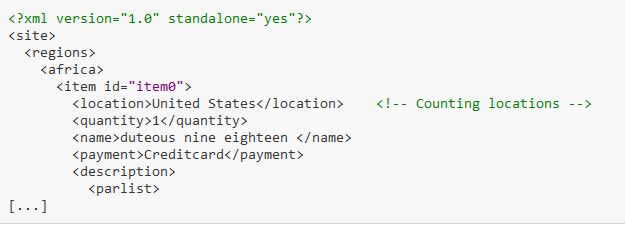
\includegraphics[width=0.75\textwidth]{figures/XML}}
	\caption{XML stream parsing dengan iterparse}
	\label{XML stream parsing dengan iterparse}
\end{figure}



\chapter{GUI Programming}
\section{GUI Programming}
\hspace*{0.5in} Python menyediakan berbagai pilihan untuk mengembangkan antarmuka pengguna grafis (GUIs). Yang paling tercantum dibawah ini : 

\begin{itemize}
\item Tkinter 

Antarmuka Python ke toolkit Tk GUI dikirimkan dengan Python.  
\item wxPython 

antarmuka Python open-source untuk wxWindows 
 
\item Jpython 

Port Python untuk java yang memberikan Python script akses tanpa batas ke perpustakaan kelas java pada mesin lokal 

\subsection{Tkinter Pemrograman} 
\hspace*{0.5in} Tkinter adalah perpustakaan GUI standar untuk Python. Python bila dikombinasikan dengan Tkinter menyediakan cara yang mudah dan cepat untuk membuat aplikasi GUI. Tkinter menyediakan antarmuka berorientasi ojek yang kuat untuk toolkit Tk GUI. 
 
\hspace*{0.5in} Membuat aplikasi GUI menggunakan Tkinter adalah tugas yang mudah. Yang diperlukan adalah melakukan langkah-langkah sebagai berikut : 
 
\item Mengimpor Tkinter modul 
\item Buat jendela utama aplikasi GUI 
\item Tambahkan satu atau lebih dari widget tersebut diatas ke aplikasi GUI 
\item Masukkan acara loop utama untuk mengambil tindakan terhadap setiap peristiwa dipicu oleh pengguna\end{itemize}
 
\vspace{12pt} 
Contoh : 
\begin{verbatim}
$  \#  $!/usr/bin/python} 
import Tkinter} 

top = Tkinter.Tk()} 

 $  \#  $ Code to add widgets will go here...} 

top.mainloop()} 
\end{verbatim}

\vspace{10pt}
\subsection{Tkinter Widget} 
\hspace*{0.5in} Tkinter menyediakan berbagai kontrol seperti tombol, label dan kotak teks yang digunakan dalam aplikasi GUI. Kontrol ini biasanya disebut widget.  
 
\hspace*{0.5in} Saat ini ada 15 jenis widget di Tkinter. Menyajikan widget serta penjelasan singkat pada tabel berikut ini : 
\vspace{100pt}


 %%%%%%%%%%%%  Table No:1 Here %%%%%%%%%%%%%%


\begin{table}[ht]
	\caption{Ukuran}
	\begin{tabular*}{\textwidth}{@{\extracolsep{\fill}}lcc}
		\hline
		Operator& Penjelasan \cr
		\hline
		Button&SMenampilkan tombol dalam aplikasi&\cr
		Canvas&Menggambar bentuk seperti garis, oval, poligon dan persegi panjang dalam aplikasi&\cr
		Checkbutton&Menampilkan sejumlah pilihan sebagai kotak centang. Pengguna dapat memilih beberapa pilihan pada suatu waktu&\cr
		Entry&Menampilka bidang garis teks tunggal untuk menerima nilai-nilai dari pengguna\cr
		Frame&Wadah untuk mengatur widget lainnya&\cr
		Label &Memberikan keterangan garis single untuk widget lainnya. Hal ini berisi gambar&\cr
		Listbox &Menyediakan daftar pilihan kepada pengguna&\cr
		Menubutton&Menampilkan menu dalam aplikasi&\cr
		Menu&Memberikan berbagai perintah untuk pengguna. Perintah-perintah ini terkandung di dalam MenuButton&\cr
		Message&Menampilkan bidang teks multiline untuk menerima nilai-nilai dari pengguna&\cr
		RadioButton&Menampilkan sejumah pilihan sebagai tombol radio. Pengguna dapat memilih hanya satu pilihan pada suatu waktu&\cr
		Scale&Menyediakan widget slide&\cr
		Scrollbar &Menambah kemampuan bergulir ke berbagai widget seperti kotak daftar&\cr
		Text&Menampilka teks dalam beberapa garis&\cr
		Toplevel&Menyediakan wajah jendela terpisah&\cr
		PanedWindow&Wadah yang mengandung sejumlah panel disusun horizontal atau vertikal&\cr
		LabelFrame&Wadah widget sederhana. Bertindak sebagai spacer atau wajah untuk layout jendela kompleks&\cr
		TkMessageBox&Menampilkan kotak pesan dalam aplikasi&\cr
		Spinbox &Memilih sejumlah tetap nilai-nilai&\cr
		\hline
	\end{tabular*}
	\begin{tablenotes}
	\end{tablenotes}
\end{table}


 %%%%%%%%%%%%  Table No:1 Ends Here %%%%%%%%%%%%%%


\vspace{12pt}
\hspace*{0.5in} Beberapa atribut sebagai ukuran, warna dan font ditentukan. Berikut adalah beberapa atribut standar : 
 
\begin{itemize}
\item Ukuran 
 
Berbagai panjang, lebar, dan dimensi lain dari widget digambarkan dalam banyak unit yang berbeda seperti : 
 
\item Jika menetapkan dimensi ke integer diasumsikan dalam piksel 
 
\item Menentukan unit dengan menentukan dimensi untuk string yang berisi sejumlah diikuti oleh :
\end{itemize}
\vspace{100pt}
 


 %%%%%%%%%%%%  Table No:2 Here %%%%%%%%%%%%%%


\begin{table}[ht]
	\caption{Ukuran}
	\begin{tabular*}{\textwidth}{@{\extracolsep{\fill}}lcc}
		\hline
		Karakter&  Penjelasan \cr
		\hline
		c&Sentimeter&\cr
		i&Inci&\cr
		m&Milimeter&\cr
		p&Poin printer\cr
		\hline
	\end{tabular*}
	\begin{tablenotes}
	\end{tablenotes}
\end{table}


 %%%%%%%%%%%%  Table No:2 Ends Here %%%%%%%%%%%%%%


\hspace*{0.5in} Tkinter mengungkapkan panjang sebagai integer jumlah piksel. Berikut ini adalah daftar pilihan panjang umum: 
 
\begin{itemize}
\item borderwidth 

Lebar batas yang memberikan tampilan tiga dimensi untuk widget 
\item highlightthickness 

Lebar puncak persegi panjang ketika widget memiliki fokus 
\item padX padY 

Ruang tambahan widget dari manajer tata letak luar minimum widget perlu menampilkan isinya di x dan y arah 
\item selectborderwidth 

Lebar perbatasan tiga dimensi disekitar dipilih item widget 
\item wraplength 

Panjang garis maksimum untuk widget yang melakukan kata membungkus 
\item height 

Tinggi diinginkan widget 
\item underline 

Indeks karakter untuk menggarisawahi dalam teks widget  
\item width 
 
\item Lebar diinginkan widget

\item Warna 
\end{itemize}
\vspace{12pt}
 
\hspace*{0.5in} Tkinter memiliki warna dengan string. Ada dua cara umum untuk menentukan warna di Tkiter, yaitu : 
 
\begin{itemize}
\item Menggunakan string menentukan proporsi merah, hijau dan biru didigit heksadesimal. Misalnya  $ " $ $  \#  $ffff $ " $ putih,  $ " $ $  \#  $000000 $ " $ hitam dan  $ " $ $  \#  $000fff000 $ " $ hijau. 
 
\item Menggunakan lokal standar nama warna . warna-warna  $ " $white $ " $, $ " $black $ " $,  $ " $green $ " $ dan  $ " $magenta $ " $ akan selalu tersedia.\end{itemize}
 
\vspace{12pt}
Pilihan warna umum : 
 
\begin{itemize}
\item activebackground 

Warna latar berlakang untuk widget ketika widget aktif 
\item activeforeground 

Warna depan untuk widget ketika widget aktif 
\item background 

Merepresentasikan sebagai \textit{bg} 
\item disableforeground 

Warna depan untuk widget ketika widget dinonaktifkan 
\item foreground 

Merepresentasikan fg 
\item highlightbackground 

Warna latar belakang dari daerah puncak ketika widget memiliki fokus 
\item hightlightcolor 

Warna depan dari wilayah puncak ketika widget memiliki fokus 
\item selectbackground 

Warna latar belakang untuk item yang dipilih dari widget 
\item selectforeground 

Warna depan untuk item yang dipilih dari widget 
\item Font 
 
Sebagai tupel yang elemen pertama adalah keluarga font diikuti dengan string yang berisi satu atau lebih gaya pengubah tebal,miring, garis bawah dan overstrike. 
\end{itemize}
 
\vspace{12pt}
\hspace*{0.5in} Dapat membuat  $ " $font object $ " $ dengan mengimpor modul tkFont dan menggunakan kelas konstruktor font nya : 
Import tkFont 
Font = tkFont.Font (option, ....) 
\vspace{12pt}
Berikut adalah daftar pilihan : 
 
\begin{itemize}
\item Family 

Font nama keluarga sebagai string 
\item Size 

Font tinggi sebagai integer dalam poin 
\item Weight 

Bold untuk teal, normal untuk berat badan secara teratur 
\item Slant 

Italic untuk miring, roman untuk unstlanted 
\item Underline 

1 untuk teks yang digarisbawahi, 0 untuk normal 
\item Overstrike 

1 untuk teks telak, 0 untuk normal 
Jika berjalan di bawah X window system, dapat menggunakan salah satu nama font X. Sebagai contoh, font bernama  $ " $-*lucidatypewriter-medium-r-*-*-*-140-*-*-* $ " $ adalah favorit fixed-width font penulis untuk digunakan pada layar. 
\item Jangkar  

Jangkar digunakan untuk mendefinisikan mana teks diposisikan relatif terhadap titik acuan. 
\end{itemize}
 
\vspace{12pt}
\hspace*{0.5in} Jika menggunakan tengah sebagai jangkar tek, tek akan ditengahkan horizontal dan vertikal disekitar titik referensi. 
Jangkar NW akan posisi teks sehingga titik referensi bertepatan dengan laut sudut kotak berisi teks 
Jangakr W akan pusat teks secara vertikal disekitar titik referensi dengan tepi kiri kotak teks yang melewati titik itu dan sebagainya. 
Jika membuat widget kecil didalam bingkai besar dan menggunakan jangkar = SE pilihan, widget akan ditempatkan disudut kanan bawah gambar. Jika menggunakan anchor = N sebaliknya widget akan dipusatkan disepanjang tepi atas. 

\hspace*{0.5in}Widget mengacu pada efek 3-D simulasi terbaru disekitar bagian luar widget. Berikut adalah daftar konstanta yang mungkin dapat digunakan untuk atribut: 
 
\begin{itemize}
\item Datar 
 
\item Dibesarkan 
 
\item Cekung 
 
\item Alur 
 
\item Punggung bukit
\end{itemize}
 
\vspace{12pt}
Contoh : 
\begin{verbatim}
From Tkinter import *} 

Import Tkinter} 

 top = Tkinter.Tk()} 
B1 = Tkinter.Button(top, text= $ " $FLAT $ " $, relief
=FLAT)} 
B2 = Tkinter.Button(top, text= $ " $RAISED $ " $, relief
=RAISED)} 
B3 =Tkinter.Button(top, text= $ " $SUNKEN $ " $, relief
=SUNKEN)} 
B4=Tkinter.Button(top, text= $ " $GROOVE $ " $, relief
=GROOVE)} 
B5=Tkinter.Button(top, text= $ " $RIDGE $ " $, relief
=RIDGE)} 

 B1.pack()} 
 B2.pack()} 
 B3.pack()} 
 B4.pack()} 
 B5.pack()} 
 top.mainloop()} 
 \end{verbatim}
 
Ada beberapa jenis bitmap yang tersedia, diantaranya:  
\begin{itemize}
\item Kesalahan 
 
\item Gray75 
 
\item Gray50 
 
\item Gray12 
 
\item Jam Pasir 
 
\item Info 
 
\item Questhead 
 
\item Perantanyaan  
 
\item Peringatan\end{itemize}
 
\vspace{12pt}
Contoh: 
\begin{verbatim}
 From Tkinter import *} 
 
 Import Tkinter} 

 Top = Tkinter.Tk()} 

 B1 = Tkinter.Button(top, text = $ " $error $ " $, relief
 =RAISED,  $    $ bitmap= $ " $error $ " $)} 
 B2 = Tkinter.Button(top, text = $ " $hourglass $ " $, relief
 =RAISED,  $    $ bitmap= $ " $hourglass $ " $)} 
 B3 = Tkinter.Button(top, text = $ " $info $ " $, relief
 =RAISED,  $    $ bitmap= $ " $info $ " $)} 
 B4 = Tkinter.Button(top, text = $ " $question $ " $, relief
 =RAISED,  $    $ bitmap= $ " $question $ " $)} 
 B5 = Tkinter.Button(top, text = $ " $warning $ " $, relief
 =RAISED,  $    $ bitmap= $ " $warning $ " $)} 

 B1.pack()} 
 B2.pack()} 
 B3.pack()} 
 B4.pack()} 
 B5.pack()} 
 top.mainloop()} 
\end{verbatim}

\vspace{12pt}
Berikut daftar menarik : 
 
\begin{itemize}
\item Panah 
 
\item Lingkaran 
 
\item Jam 
 
\item Menyebrang 
 
\item Dotbox 
 
\item Bertukar 
 
\item Fluer 
 
\item Jantung 
 
\item Manusia 
 
\item Tikus 
 
\item Bajak laut 
 
\item Tamah 
 
\item Antar jemput 
 
\item Perekat 
 
\item Laba-laba 
 
\item Kaleng semprot 
 
\item Bintang 
 
\item Target 
 
\item Tcross 
 
\item Melakukan perjalanan 
 
\item Menonton
\end{itemize}
 
\vspace{12pt}
Contoh : 
\begin{verbatim}
From Tkinter import *} 

Import Tkinter} 

Top = Tkinter.Tk()} 

B1 = Tkinter.Button(top, text = $ " $circle $ " $, relief
=RAISED,  $    $ bitmap= $ " $circle $ " $)} 
B2 = Tkinter.Button(top, text = $ " $plus $ " $, relief
=RAISED,  $    $ bitmap= $ " $plus $ " $)} 

B1.pack()} 
B2.pack()} 
font top.mainloop()} 
\end{verbatim}

\vspace{10pt}
\subsection{Manajemen Geometri} 
 
\hspace*{0.5in} Semua widget tkinter memiliki akses ke metode manajemen geometri tertentu, yang memiliki tujuan menggorganisir widget diseluruh wilayah widget induk. Tkinter mengekspos kelas manager geometri berikut : 
 
\begin{itemize}
\item Metode the \textit{pack()} 
 
Manajer geometri ini mengatur widget diblok sebelum menempatkan mereka di widget induk 
\item Metode the \textit{grid()} 
 
Manajer geometri ini mengatur widget dalam struktur tabel seperti di widget induk 
\item Metode~the  \textit{place()}\end{itemize}
  
Manajer geometri ini mengatur widget dengan menempatkan dalam posisi tertentu dalam widget induk 
\vspace{12pt}
 
\subsection{Manfaat Tkinter} 
\hspace*{0.5in} Tkinter sangat sederhana. Erikut manfaat Tkinter dibandingkan GUI toolkit : 
 
\begin{itemize}
\item Tkinter mudah diakses oleh siapa saja (Accessibilty)

Tkinter merupakan toolkit yang ringan dan satu-satunya solusi GUI yang paling sederhana untuk Python sampai saat ini. Cukup menuliskan beberapa baris kode Python untuk membuat aplikasi GUI sederhana dengan Tkinter. Untuk menambahkan komponen baru pada Tkinter, dapat membuatnya dalam kode Python atau menambahkan paket ekstensi seperti Pmw, Tix, atau ttk. 
\item Tkinter mudah digunakan di semua platform (Portability)

Sebuah program Python yang dibangun menggunakan Tkinter dapat berjalan dengan baik di semua platform sistem operasi seperti Microsoft Windows, Linux, dan Macintosh. Dan dari segi tampilan window, akan terlihat sama dengan standar platform yang digunakan. 
 
\item Tkinter selalu tersedia di Python (Availability)

Tkinter merupakan modul standar pada pustaka Python. Sebagian besar paket instalasi Python sudah langsung berisi Tkinter. Khusus untuk beberapa distro Linux, perlu menambahkan paket Tkinter secara terpisah. Pada Windows, bisa langsung menggunakan Tkinter sesaat setelah menginstal paket instalasi Python. 
 
\item Dokumentasi Tkinter (Documentation)

Python (plus Tkinter) ini bersifat open-source, maka banyak sekali komunitas-komunitas yng membahas Python dan Tkinter dan bisa belajar dan bertanya langsung dengan para ahli
\end{itemize}

\section{Contoh GUI Programming}
\hspace*{0.5in} Dalam contoh ini, menulis naskah yang membuka jendela yang memiliki dua kotak masuk diantaranya satu nama depan berlabel dan nama belakang lainnya. Jendela memiliki dua tombol yaitu Greeting yang menampilkan kotak pesan selamat datang ke pengguna dan Close yang menutup aplikasi

\begin{verbatim}
import tkinter
from tkinter import *

det DisplayMsgBox():

    tkinter.messagebox.showinfo("Your Name", "Welcome"+ 
    Entry.get()+ "" +Entry2.get())

mainwindow = Tk()
Label(mainwindow, text="Firstname").grid(row=0)
Label(mainwindow, text="Lastname").grid(row=0)

Entry1 = Entry(mainwindow)
Entry2 = Entry(mainwindow)

Entry1.grid(row=0, column=1)
Entry2.grid(row=1, column=1)
Entry1.focus()

Button(mainwindow, text='Greeting', command=DisplayMsgBox)
.grid(row=3, column=0)
Button(mainwindow, text='Close', command=DisplayMsgBox)
.grid(row=3, column=1)

mainloop()
\end{verbatim}

\vspace{12pt}
Ketik nama depan dan nama belakang, lalu tekan "Greeting", \ref{Contoh} Lihat Contoh dibawah ini :
\begin{figure}[ht]
	\centerline{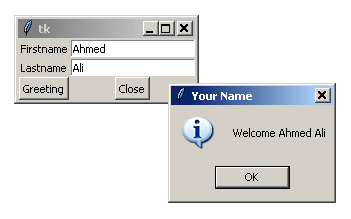
\includegraphics[width=0.70\textwidth]{figures/Contoh}}
	\caption{Contoh}
	\label{Contoh}
\end{figure}

\vspace{12pt}
Tekan "Close" akan menghentikan aplikasi 

*******

\vspace{12pt}
\hspace*{0.5in} Tkinter berisi sebagian besar kelas dan metode yang dibutuhkan untuk membuat aplikasi GUI yang bagus. Menggunakan kelas Tk untuk membuat master (jendela utama) dan instantiated objek untuk memasukkan berbagai kontrol pada jendela aplikasi.



\chapter{Futher Expression}
\section{Further Expression}
\hspace*{0.5in} Setiap kode yang dituliskan menggunakan bahasa yang dikompilasi seperti C, C++ atau Java dapat diintegrasikan ke skrip Python lainnya. Kode ini dianggap sebagai ektensi. 

\hspace*{0.5in} Modul ekstensi Python tidak lebih dari sekedar perpustakaan C biasa. Pada mesin Unix, perpustakaan ini biasanya diakhiri dengan .so (untuk objek bersama). Pada mesin windows, biasanya melihat .dll (untuk perpusatkaan yang terhubung secara dinamis).  


\subsection{Pra-Persyaratan untuk Menulis Ekstensi} 

\hspace*{0.5in} Untuk memulai ektensi, memerlukan file header Python. Pada mesin Unix, biasanya memerlukan instalasi paket khusus pengembang seperti python 2-5. 

\hspace*{0.5in} Pengguna window mendapatkan header ini sebagai bagian dari paket saat menggunakan pemasang Python biner. 

\hspace*{0.5in} Harus memiliki pengetahuan yang baik tentang C atau C++ untuk menulis ekstensi Python menggunakan pemrograman C. 
 
\hspace*{0.5in} Untuk melihat modul ekstensi Python, perlu mengelompokkan kode menjadi empat bagian : 

\begin{itemize}
\item File header Python 
\item Fungsi C yang ingin ditampilkan sebagai antarmuka dari modul 
\item Sebuah tabel memetakan nama-nama fungsi saat pengembang Python melihat ke fungsi C didalam modul ekstensi 
\item Fungsi inilisasi
\end{itemize}
 
\vspace{12pt}
\hspace*{0.5in} Perlu menyertakan file header Python.h di file sumber C memberi akses ke API Python internal digunakan untuk menghitung modul ke penerjamah. 
Menyertakan header Python.h sebelum header lain yang mungkin dibutuhkan. Mengikuti termasuk dengan fungsi yang ingin dipanggil dari Python. 
Tanda tangan penerapan C fungsi selalu mengambil salah satu dari tiga bentuk berikut : 


\begin{verbatim}
static PyObject *MyFunction( PyObject *self, PyObject *ar
gs);} 
 
static PyObject *MyFunctionWithKeywords(PyObject *self,} 

                                        PyObject *args,} 

                                        PyObject *kw);} 
                                        
static PyObject *MyFunctionWithNoArgs( PyObject *self );} 
\end{verbatim}

\vspace{12pt}
\hspace*{0.5in} Masing-masing deklarasi seelumnya mengembalikan objek Python. Tidak ada yang namanya fungsi void dengan Python seperti ada di C. Jika ingin fungsi mengembalikan nilai, Python. Header Python mendefinisikan makro.  

\hspace*{0.5in} Nama-nama fungsi C bisa menjadi apapun yang disuka karena tidak pernah diluar modul ekstensi mendefinisikan sebagai statis. 

\hspace*{0.5in} Fungi Cbiasanya diberi nama dengan menggabnungkan modul dan fungsi Python bersama-sama yang ditunjukan disini : 


\begin{verbatim}
static PyObject *{module $  \_  $func}(PyObject *self, 
PyObject *args) $ \{ $ 

    /* Do your stuff here. */ 

    Py $  \_  $RETURN $  \_  $NONE; 

 $  \}  $ 
\end{verbatim}

\vspace{12pt}
\hspace*{0.5in} Ini adalah fungsi Python yang disebut func didalam modul-modul. Memasukkan petunjuk ke fungsi C ke dalam tabel metode untuk modul yang biasanya muncul selanjutnya dikode sumber tael pemetaan metode. 

\hspace*{0.5in} Tabel metode ini adalah susunan sederhana dari struktur PyMethodSef. Struktur itu terlihat seperti ini : 

\begin{verbatim}
struct PyMethodDef  $  \{  $ 
 
   char *ml $  \_  $name; 
 
   PyCFunction ml $  \_  $meth; 

   int ml $  \_  $flags; 
 
   char *ml $  \_  $doc; 

 $  \}  $; 
\end{verbatim}

\vspace{12pt}
Ini nilai uraian anggota struktur ini : 

\begin{itemize}
\item Ml $  \_  $name 

Nama fungsi yang digunakan penafsir Python saat digunakan dalam program Python 
\item Ml $  \_  $meth 

Menjadi alamaat ke fungsi yang memiliki salah satu tanda tangan yang dijelaskan dalam penelusuran sebelumnya 
\item Ml $  \_  $flags 

Memberitahu penafsir yang mana dari tiga tanda tangan yang digunakan ml $  \_  $meth. Bendera ini biasanya mmiliki nilai meth $  \_  $varargs. Bendera ini dapat digandakan dengan or’ed dengan meth $  \_  $keywords jika ingin memiarkan argumen kata kunci masuk ke fungsi. Ini juga bisa memiliki nilai meth $  \_  $noargs yang menunjukan bahwa tidak ingin menerima argumen apa pun. 
\item Ml $  \_  $doc 

Ini adalah docstring untuk fungsi yang bisa jadi NULL jika tidak ingin menulisnya. 
\vspace{12pt}

\hspace*{0.5in} Tabel ini perlu diakhiri dengan sentinel yang terdiri dari NULL dan 0 untuk anggota yang sesuai. 
\vspace{12pt}

Contoh: 
\begin{verbatim}
static PyMethodDef {module} $  \_  $methods[] 
=  $  \{  $ 

   $  \{  $ "{func}", (PyCFunction){module $
\_  $func}, METH $  \_  $NOARGS, NULL  $  \}  $, 

   $  \{  $ NULL, NULL, 0, NULL  $  \}  $ 

 $  \}  $; 
\end{verbatim}

\vspace{12pt}
\hspace*{0.5in} Bagian terakhir dari modul ekstensi adalah fungsi inialisasi. Fungsi ini dipanggil oleh juru bahasa Python saat modul diisikan. Hal ini diperlukan agar fungsi diberi nama intiModule dimana modul adalah nama modul. 

\hspace*{0.5in} Fungsi inialisasi perlu diekspor dari perpustakaan yang akan dibangun. Header Python mendefinisikan PyMODINIT $  \_  $Func untuk memasukkan mantra yang sesuai agar terjadi pada lingkungan tertentu tempat menyuusun. Yang harus dilakukan adalah mengunakan saat menentukan fungsinya. Fungsi inialisasi C umumnya memiliki strktur keseluruhan berikut : 
\begin{verbatim}
PyMODINIT $  \_  $FUNC init{Module}()  $  \{  $ 

   Py $  \_  $InitModule3({func}, {module} $  \_ 
   $methods, "docstring..."); 

 $  \}  $ 
\end{verbatim}

\vspace{12pt}
Berikut adalah penjelasan fugsi Py $  \_  $IntiModule : 
\item Func  

Ini adalah fungsi yang akan diekspor 
\item Module 

Ini adalah nama tabel pemetaan yang didefinisikan diatas 
\item Docstring

Ini adalah komentar yang ingin diberikan diekstensi 
\end{itemize}

\vspace{12pt}
Menempatkan ini semua bersama-sama terlihat sebagai berikut : 
\begin{verbatim}
 $  \#  $include <Python.h>

static PyObject *{module $  \_  $func}(PyObject *self, 
PyObject *args)  $  \{  $ 

   /* Do your stuff here. */ 

   Py $  \_  $RETURN $  \_  $NONE; 

 $  \}  $ 
 
static PyMethodDef {module} $  \_  $methods[] =  $ 
\{  $ 

    $  \{  $ "{func}", (PyCFunction){module $  \_ 
    $func}, METH $  \_  $NOARGS, NULL  $  \}  $, 
 
    $  \{  $ NULL, NULL, 0, NULL  $  \}  $ 

 $  \}  $; 

PyMODINIT $  \_  $FUNC init {Module}()  $  \{  $ 
 
   Py $  \_  $InitModule3({func}, {module} $  \_ 
   $methods, "docstring..."); 

 $  \}  $ 
\end{verbatim}

\vspace{12pt}
Contoh: 
\begin{verbatim} 
 $  \#  $include <Python.h> 
 
static PyObject* helloworld(PyObject* self) 

 $  \{  $ 
 
   return Py $  \_  $BuildValue("s", "Hello, Python 
   extensions!!"); 

 $  \}  $ 
 
static char helloworld $  \_  $docs[] = 
static PyMethodDef helloworld $  \_  $funcs[] =  $  
\{  $ 

    $  \{  $"helloworld", (PyCFunction)helloworld,  

    METH $  \_  $NOARGS, helloworld $  \_  $docs $  
    \}  $, 

    $  \{  $NULL $  \}  $
 
 $  \}  $; 
 
void inithelloworld(void) 
 
 $  \{  $ 

   Py $  \_  $InitModule3("helloworld", helloworld $  
   \_  $funcs, 

             "Extension module example!"); 
 
 $  \}  $ 
\end{verbatim}

\vspace{12pt} 
\hspace*{0.5in} Disini fungsi Py $  \_  $BuildValue digunakan untuk membangun nilai Python.  

\vspace{12pt} 
\subsection{Membangun dan Menginstal Ekstensi} 

\hspace*{0.5in} Paket membuatnya sangat mudah mendistribusikan modul Python, baik Python murni dan modul ekstensi dengan cara standar. Modul didistribusikan dalam bentuk sumber dan dibangun dan diinstal melalui skrip setup yang iasa disebut setup.py sebagai berikut : 
 
\begin{verbatim}
from distutils.core import setup, Extension \par
      ext $  \_  $modules=[Extension('helloworld', 
      ['hello.c'])]). 
\end{verbatim}

\vspace{12pt}
\hspace*{0.5in} Sekarang gunakan perintah berikut yang aka melalakukan semua kompilasi dan langkah penghubunh yang diperlukan dengan perintah dan bendera penyusun dan penghubung yang benar dan menyalin perpustakaan dinamis yang dihasilkan ke dalam direktori yang sesuai . 
\vspace{12pt}
 
Contoh : 
\begin{verbatim}
$  \$  $ python setup.py install
\end{verbatim}
  
\vspace{12pt}
\hspace*{0.5in} Pada sistem berbasis Unix kemungkinan besar perlu menjalankan perintah ini sebagai root agar meminta izin untuk menulis ke direktori paket situs. Ini biasanya tidak menjadi masalah pada window. 
Setelah~menginstal ekstensi, akan dapat mengimpor dan memanggil ekstensi tersebut di skrip Python  sebagai berikut : 
\begin{verbatim}
$  \#  $!/usr/bin/python

  import helloworld 

  print helloworld.helloworld() 
\end{verbatim}

\vspace{12pt}
Ini akan menghasilkan hasil sebagai berikut  : 
Hello, Python extensions!! 

\vspace{12pt}
Seperti kemungkinan besar ingin mendefinisikan fungsi yang menerima argumen, dapat menggunakan salah satu tanda tangan lain untuk fungsi C. Sebagai contoh, fungsi berikut yang menerima beberapa parameter akan didefinisikan seperti ini : 
\begin{verbatim}
static PyObject *{module $  \_  $func}(PyObject 
*self, PyObject *args)  $  \{  $ 

    /* Parse args and do something interesting here. */ 

    Py $  \_  $RETURN $  \_  $NONE; 

 $  \}  $ 
\end{verbatim}

\vspace{12pt}
Tabel metode yang berisi entri untuk fungsi baru akan terlihat seperti ini : 
\begin{verbatim}
static PyMethodDef {module} $  \_  $methods[] =  $  
\{  $ 

    $  \{  $ "{func}", (PyCFunction) {module
    $  \_  $func}, METH $  \_  $NOARGS, NULL  $  \}  $, 

    $  \{  $ "{func}", {module $  \_  $func
    }, METH $  \_  $VARARGS, NULL  $  \}  $, 

    $  \{  $ NULL, NULL, 0, NULL  $  \}  $ 

 $  \}  $; 
\end{verbatim}

\vspace{12pt}
Menggunakan fungsi API PyArg $  \_  $ParseTuple untuk mengekstrak argumen dari satu pointer PyObject yang dikirimkan ke fungsi C. Argumen pertama untuk PyArg $  \_  $ParseTuple adalah args argumen. Ini adalah objek yang akan parsing. Argumen kedua adalah string format yang menggambarkan argumen saat mengharapkannya muncul. Setiap argumen diwakili oleh satu atau lebih karakter dalam format string sebagai berikut : 

\begin{verbatim}
static PyObject *{module $  \_  $func}(PyObject *self, 
PyObject *args)  $  \{  $ 

    int i;

   double d; 

   char *s; 
   
   if (!PyArg $  \_  $ParseTuple(args, "ids",  $  \&  $i,
   $  \&  $d,  $  \&  $s))  $  \{  $ 

   return NULL; 

   $  \}  $ 

   /* Do something interesting here. */ 

   Py $  \_  $RETURN $  \_  $NONE; 

   $  \}  $ 
\end{verbatim}

\vspace{12pt}
Mengkompilasi versi baru dari modul dan mengimpornya memungkinkan untuk memanggil fungsi baru dengan sejumlah argumen dari jenis apa pun : 
\begin{verbatim}
module.func(1, s="three", d=2.0) 

module.func(i=1, d=2.0, s="three") 

module.func(s="three", d=2.0, i=1) 

\end{verbatim}
\vspace{12pt}
\hspace*{0.5in} Berikut adalah tanda tangan standar untuk 
fungsi PyArg $  \_  $ParseTuple: 
 
\begin{verbatim}
int PyArg $  \_  $ParseTuple(PyObject* tuple,char* format,...) 
\end{verbatim}

\vspace{10pt}
\hspace*{0.5in} Fungsi ini mengembalikan 0 untuk kesalahan, dan nilai tidak sama dengan 0 untuk kesuksesan. Tuple adalah PyObject * yang merupakan argumen kedua dari fungsi C. Format berikut adalah string C yang menggambarkan argumen wajib dan opsional. Berikut adalah daftar kode format untuk fungsi PyArg $  \_  $ParseTuple: 

 %%%%%%%%%%%%  Table No:1 Here %%%%%%%%%%%%%%


\begin{table}[ht]
	\caption{Ukuran}
	\begin{tabular*}{\textwidth}{@{\extracolsep{\fill}}lcc}
		\hline
		Karakter&  Penjelasan \cr
		\hline
		c&Sentimeter&\cr
		i&Inci&\cr
		m&Milimeter&\cr
		p&Poin printer\cr
		\hline
	\end{tabular*}
	\begin{tablenotes}
	\end{tablenotes}
\end{table}

%%%%%%%%%%%%  Table No:1 Ends Here %%%%%%%%%%%%%%

\vspace{80pt}
Py $  \_  $BuildValue~mengambil format string seperti PyArg $  \_  $ParseTuple. Alih-alih menyampaikan alamat nilai yang sedang  bangun, melewati nilai sebenarnya. Berikut adalah contoh yang menunjukkan bagaimana menerapkan fungsi tambah : 

\begin{verbatim}
static PyObject *foo $  \_  $add(PyObject *self, PyObject 
*args)  $  \{  $ 

   int a; 

   int b; 
\vspace{12pt}

   if (!PyArg $  \_  $ParseTuple(args, "ii",  $  \&  $a,
   $  \&  $b))  $  \{  $ 

    return NULL;

    $  \}  $ 

    return Py $  \_  $BuildValue("i", a + b); 

 $  \}  $ 

 def add(a, b):

 return (a + b) 

 static PyObject *foo $  \_  $add $  \_  $subtract(PyObject 
 *self, PyObject *args)  $  \{  $ 

  int a; 

  int b; 

  if (!PyArg $  \_  $ParseTuple(args, "ii",  $  \&  $a,  $  
  \&  $b))  $  \{  $ 

  return NULL; 

  $  \}  $ 

  return Py $  \_  $BuildValue("ii", a + b, a - b); 

 $  \}  $ 

  def add $  \_  $subtract(a, b): 

  return (a + b, a - b) 
\end{verbatim}  

\vspace{10pt}
Berikut daftar tabel string kode yang umum digunakan, yang nol atau lebihnya digabungkan ke dalam format string : 


 %%%%%%%%%%%%  Table No:2 Here %%%%%%%%%%%%%%


\begin{table}[ht]
	\caption{Ukuran}
	\begin{tabular*}{\textwidth}{@{\extracolsep{\fill}}lcc}
		\hline
		Code& C Type&  Meaning\cr
		\hline
		c&char&String Python dengan panjang 1 menjadi huruf C.\cr
		d&double&Pelampung Python menjadi C ganda.\cr
		f&float&Pelampung Python menjadi pelampung C.\cr
		i&int&Int Python menjadi int int\cr
		l&long&Sebuah int Python menjadi panjang C.\cr
		L&long long&Sebuah int Python menjadi C panjang panjang\cr
		O&PyObject*&Gets non-NULL meminjam referensi ke argumen Python\cr
		s&char*&Python string tanpa nulls tertanam ke C char *\cr
		s&char*+int&Setiap string Python ke alamat dan panjang C\cr
		t&char*+int&Read-only penyangga segmen tunggal ke alamat C dan panjangnya\cr
		U&PyUNICODE*&Python Unicode tanpa nulls tertanam ke C\cr
		u&PPyUNICODE*int+&Setiap alamat dan panjang Python Unicode C\cr
		w&char*+int&Membaca / menulis penyangga segmen tunggal ke alamat dan panjang C\cr
		Z&char*&Seperti s, juga menerima None (set C char * ke NULL).\cr
		z&char*+int&Seperti s, juga menerima None set C char * ke NULL\cr
		(...)&Poin printer&Urutan Python diperlakukan sebagai satu argumen per item.\cr
		|&as per ...&Argumen berikut bersifat opsional.\cr
		:&&Format akhir, diikuti dengan nama fungsi untuk pesan error.\cr
		;&&Format akhir, diikuti oleh seluruh pesan kesalahan teks.\cr				
		\hline
	\end{tabular*}
	\begin{tablenotes}
	\end{tablenotes}
\end{table}


 %%%%%%%%%%%%  Table No:2 Ends Here %%%%%%%%%%%%%%


\vspace{12pt}
Kode  $  \{  $... $  \}  $ membangun kamus dari sejumlah nilai C, kunci dan nilai bergantian. Misalnya, Py $  \_  $BuildValue (" $  \{  $issi $  \}  $", 23, "zig", "zag", 42) mengembalikan kamus seperti  $  \{  $23: 'zig', 'zag': 42 $  \}  $ Python. Setiap blok memori yang dialokasikan dengan malloc () pada akhirnya harus dikembalikan ke genangan memori yang tersedia dengan satu panggilan untuk membebaskan (). Penting untuk menelepon gratis () pada waktu yang tepat. Jika alamat blok dilupakan tapi gratis () tidak dipanggil untuk itu, memori yang ditempatinya tidak dapat digunakan kembali sampai program berakhir. Ini disebut kebocoran memori. Di sisi lain, jika sebuah program memanggil gratis () untuk satu blok dan kemudian terus menggunakan blok tersebut, itu menciptakan konflik dengan penggunaan ulang blok melalui panggilan malloc () yang lain. Ini disebut dengan menggunakan memori yang dibebaskan. Ini memiliki konsekuensi buruk yang sama seperti merujuk pada data yang tidak diinisiasi - dump inti, hasil yang salah, crash misterius. Karena Python membuat penggunaan malloc () dan gratis (), dibutuhkan strategi untuk menghindari kebocoran memori dan juga penggunaan memori yang bebas. Metode yang dipilih disebut penghitungan referensi. Prinsipnya sederhana: setiap objek berisi sebuah counter, yang bertambah saat referensi ke objek disimpan di suatu tempat, dan yang dikurangi saat referensi itu dihapus. Saat counter mencapai nol, referensi terakhir ke objek telah dihapus dan objeknya dibebaskan. 

\section{Simbol Further Expression}
\hspace*{0.5in} Simbol khusus yang paling penting adalah garis miring terbalik yang digunakan untuk dua tujuan. Pertama, backslash dapat digunakan untuk membuat lebih banyak karakter meta dalam ekspresi reguler. Kedua, jika simbol khusus diawali dengan garis miring terbalik, maka artinya khusus akan dihapus dan dengan demikian menghasilkan kecocokan literal dari simbol khusus tersebut.  Garis miring terbalik menciptakan beberapa masalah karena merupakan simbol khusus dengan ekspresi Python dan juga string Python. Ekspresi hanya akan menghasilkan kecocokan untuk \t. Untuk mengatasi masalah ini, ekspresi Python menggunakan notasi string mentah yang membuat ekspresi tetap sederhana. Dalam notasi string mentah, setiap string ekspresi diawali dengan r sehingga tidak perlu menambahkan backslash beberapa kali.Berikut \ref{SimbolFurhertExpression} SimbolFurhertExpression :
\vspace{12pt}

\begin{figure}[ht]
	\centerline{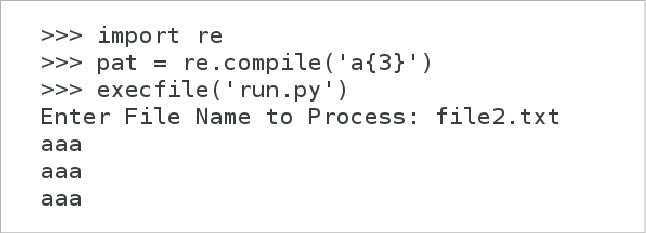
\includegraphics[width=0.50\textwidth]{figures/SimbolFurhertExpression}}
	\caption{SimbolFurhertExpression}
	\label{SimbolFurhertExpression}
\end{figure}

\vspace{12pt}
\hspace*{0.5in}Simbol adalah operator atau ekspresi biasa. Simbol khusus, tanda kurung tutup dan penutup, digunakan untuk mencari pola berulang. 





\bibliographystyle{IEEEtran}
\bibliography{loop,reference,DictionaryMicin}


%%%%%%%%%%%%%%%
%%  The default LaTeX Index
%%  Don't need to add any commands before \begin{document}
\printindex

%%%% Making an index
%% 
%% 1. Make index entries, don't leave any spaces so that they
%% will be sorted correctly.
%% 
%% \index{term}
%% \index{term!subterm}
%% \index{term!subterm!subsubterm}
%% 
%% 2. Run LaTeX several times to produce <filename>.idx
%% 
%% 3. On command line, type  makeindx <filename> which
%% will produce <filename>.ind 
%% 
%% 4. Type \printindex to make the index appear in your book.
%% 
%% 5. If you would like to edit <filename>.ind 
%% you may do so. See docs.pdf for more information.
%% 
%%%%%%%%%%%%%%%%%%%%%%%%%%%%%%

%%%%%%%%%%%%%% Making Multiple Indices %%%%%%%%%%%%%%%%
%% 1. 
%% \usepackage{multind}
%% \makeindex{book}
%% \makeindex{authors}
%% \begin{document}
%% 
%% 2.
%% % add index terms to your book, ie,
%% \index{book}{A term to go to the topic index}
%% \index{authors}{Put this author in the author index}
%% 
%% \index{book}{Cows}
%% \index{book}{Cows!Jersey}
%% \index{book}{Cows!Jersey!Brown}
%% 
%% \index{author}{Douglas Adams}
%% \index{author}{Boethius}
%% \index{author}{Mark Twain}
%% 
%% 3. On command line type 
%% makeindex topic 
%% makeindex authors
%% 
%% 4.
%% this is a Wiley command to make the indices print:
%% \multiprintindex{book}{Topic index}
%% \multiprintindex{authors}{Author index}

\end{document}

